\chapter{呼吸系统疾病}

\section{急性上呼吸道感染}

急性上呼吸道感染(upper respiratory tract
infection,简称上感)是鼻腔、咽或咽喉部急性炎症的概称。大多由病毒引起,少数为细菌所致,是最常见的一种传染性疾病,传染性强,有时可引起较重的并发症,如中耳炎、支气管炎、肺炎、心肌炎等。本病全年皆可发病,多数为散发,亦可流行。根据病因不同,其临床表现可多样。

【治疗程序】 图\ref{fig1-1-1}所示。

\begin{figure}[!htbp]
 \centering
 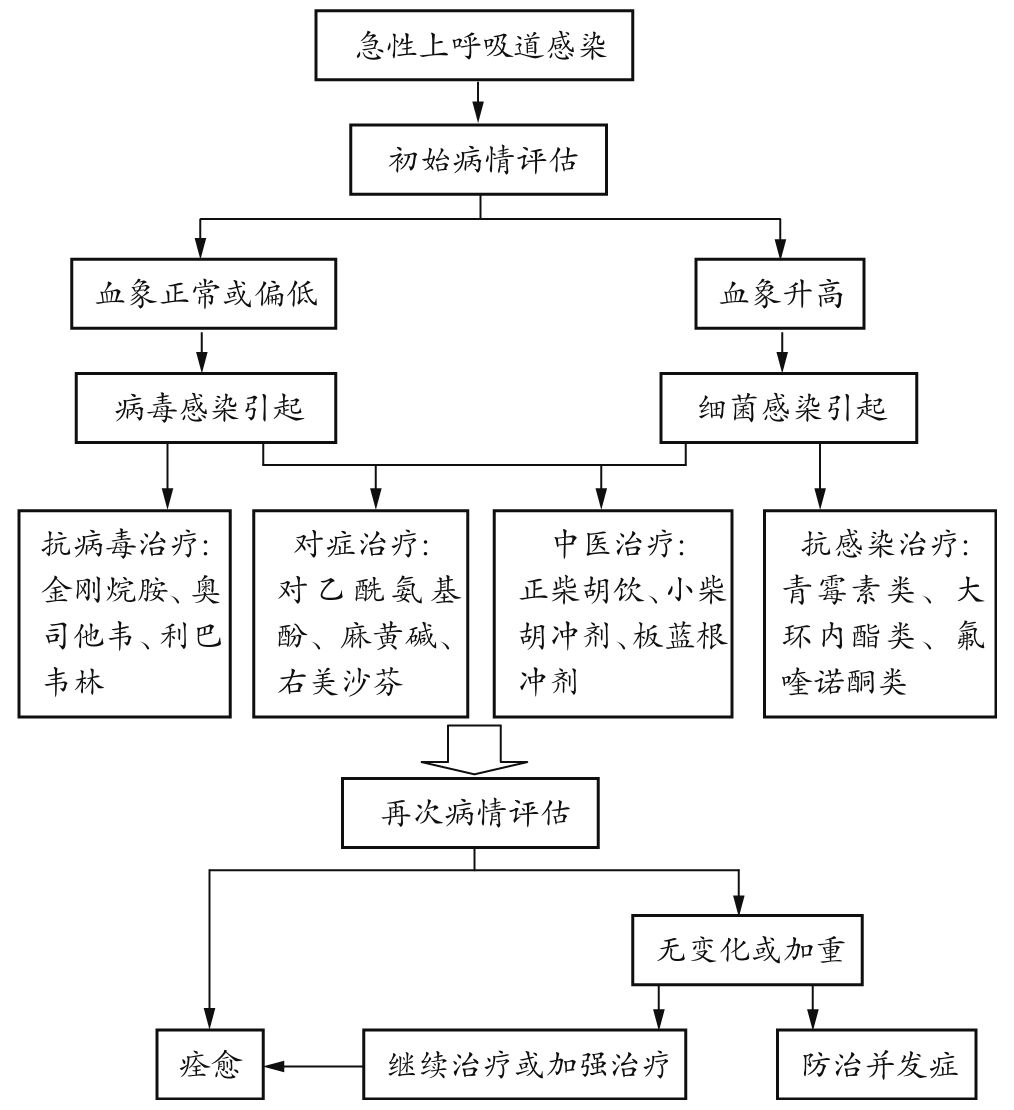
\includegraphics{./images/Image00000.jpg}
 \captionsetup{justification=centering}
 \caption{急性上呼吸道感染的治疗程序}
 \label{fig1-1-1}
  \end{figure} 

【治疗方案】

{(一)一般治疗}
 注意休息,发热、病情较重或年老体弱的患者应卧床休息。忌烟,多饮水,保持室内空气流通。

{(二)药物治疗}

1. 对症治疗

(1)解热镇痛:有头痛、发热、周身肌肉酸痛症状者,可酌情应用解热镇痛药如对乙酰氨基酚、阿司匹林、布洛芬等,如必要时予阿司匹林0.3g口服。

(2)减充血:有鼻塞、鼻粘膜充血、水肿、咽痛等症状者,可应用盐酸伪麻黄碱等可选择性收缩上呼吸道粘膜血管的药物,也可用1\%麻黄碱滴鼻,如1\%麻黄碱每次1\textasciitilde{}2滴滴鼻,每日3次。

(3)抗过敏:有频繁喷嚏、多量流涕等症状的患者,可酌情选用马来酸氯苯那敏或苯海拉明等抗过敏药物,如马来酸氯苯那敏4mg口服,每晚1次。为了减轻这类药物引起头晕、嗜睡等不良反应,宜在临睡前服用。

(4)镇咳:对于咳嗽症状较为明显者,可给予右美沙芬、喷托维林(咳必清)等镇咳药,如咳必清25mg口服,每日3次。

2.
抗病毒感染 吗啉胍对流感病毒、腺病毒和鼻病毒等有一定的疗效;广谱抗病毒药利巴韦林和奥司他韦对流感病毒、副流感病毒、呼吸道合胞病毒均有较强的抑制作用,主张早期使用,可缩短病程。如利巴韦林含片50mg含服,每日4\textasciitilde{}6次。

3.
抗细菌感染 如有细菌感染,可酌情选用适当的抗感染药物,如青霉素类、大环内酯类、氟喹诺酮类(环丙沙星、左氧氟沙星)等。如乙酰螺旋霉素0.2g口服,每日3次。对于单纯病毒感染者不应用抗菌药物。

4.
中医治疗 根据中医辨证施治的原则,应用中药治疗本病有一定疗效。正柴胡饮冲剂、小柴胡冲剂和板蓝根冲剂等在临床应用较为广泛。如正柴胡饮冲剂5g口服,每日3次。

【疗效观察与随访】

1. 观察指标 常见症状与体征、血常规、病原学检查等。

2. 治愈标准 症状、体征消失,相关检测指标恢复正常,无并发症。

3. 随访 注意病情观察,避免并发症。

【治疗经验与解析】

1.
急性上呼吸道感染以病毒引起者最为常见而且多数系自限性疾病,因此,一般情况下不必应用抗生素。鼻病毒是引起普通感冒的常见病原体,而目前对鼻病毒尚无有效、安全的抗病毒药物,因此本病的治疗以对症治疗为主。

2.
老人、儿童和有基础疾病(如慢性阻塞性肺疾病、肝硬化等)的患者易引起心肌炎、肺炎、肾炎和风湿病等并发症,因而在治疗过程中应密切观察病情变化,警惕并发症的发生。

3.
合并细菌感染的患者,可出现高热,白细胞明显升高和(或)扁桃体化脓性病变等,可酌情给予抗生素口服或静脉滴注,如青霉素类、大环内酯类或头孢菌素类等。


\section{急性气管-支气管炎}

急性气管-支气管炎(acute
tracheobronchitis)是由感染、物理化学刺激或过敏引起的气管-支气管粘膜急性炎症。常发生在寒冷季节或气温突然变冷时。临床上以咳嗽、咳痰为主要症状。先为干咳或少量粘液性痰,后可转化为粘液脓性,痰量增多,咳嗽加剧,偶可痰中带血,支气管痉挛时可有不同程度的胸闷、气急。体检两肺呼吸音增粗,部位不固定的散在的干、湿啰音,咳痰后可减少或消失,可有低、中度发热,白细胞计数和中性粒细胞可不增高或轻度增高,胸部X线检查多数表现为肺纹理增粗,少数病例无异常表现。咳嗽和咳痰可延续3周才消失。

【治疗程序】 图\ref{fig1-2-1}所示。

\begin{figure}[!htbp]
 \centering
 
\includegraphics{./images/Image00001.jpg}
 \captionsetup{justification=centering}
 \caption{急性气管-支气管炎的治疗程序}
 \label{fig1-2-1}
  \end{figure} 

【治疗方案】

{(一)一般治疗}
 患者应休息至体温正常,注意保暖。发热期间鼓励适当多喝水,忌烟。

{(二)药物治疗}

1. 对症治疗

(1)镇咳:可酌情应用右美沙芬、咳必清或苯丙哌林等镇咳剂,如咳必清25mg口服,每日3次。但对于有痰的患者不宜给予可待因等强力镇咳药,以免影响痰液排出。

(2)祛痰:除了复方氯化铵、溴己新、乙酰半胱氨酸和鲜竹沥等常用祛痰药外,近年来,盐酸氨溴索、标准桃金娘油也广泛应用,如盐酸氨溴索30mg口服,每日3次。

(3)解痉、抗过敏:对于发生支气管痉挛的患者,可给予解痉平喘和抗过敏药物,如氨茶碱0.1g口服,每日3次,马来酸氯苯那敏4mg口服,每日1次。

2.
抗菌药物治疗 一般可选用青霉素类、大环内酯类(红霉素、罗红霉素、阿奇霉素等)、氟喹诺酮类(环丙沙星、左氧氟沙星)等,必要时可应用第1代或第2代头孢菌素等。一般为口服或肌注,必要时可静脉滴注。如罗红霉素0.15g口服,每日2次,或者左氧氟沙星0.5g静脉滴注,每日1次。

【疗效观察与随访】

1. 观察指标

(1)症状、体征:观察咳嗽、咳痰的缓解情况,痰量、痰液性状的变化,胸闷、气急的好转状况。注意观察体温,两肺呼吸音以及啰音的变化等。

(2)血常规:可监测血象变化,决定是否继续抗感染治疗。

(3)病原学检查:必要时可予细菌培养和药敏试验等。

2. 疗效评估 治愈标准:症状、体征消失,相关检测指标恢复正常,无并发症。

3. 随访 注意病情观察,避免并发症。

【治疗经验与解析】

1.
本病可并发肺炎或发展为慢性支气管炎,必须重视,但临床医生在治疗急性气管-支气管炎患者时应避免滥用抗生素。应用抗生素的指征是患者出现发热、脓性痰和重症咳嗽。另外,近年来因肺炎支原体和肺炎衣原体感染引起的急性气管-支气管炎也趋多见,抗感染治疗时应注意药物抗菌谱。

2.
本病可以由病毒感染所致,注意区别。另外,在流行性感冒流行期间,如有急性气管-支气管炎的表现,应该应用抗流感的治疗措施。


\section{慢性支气管炎}

慢性支气管炎(chronic
bronchitis,简称慢支)是指气管、支气管粘膜及其周围组织的慢性非特异性炎症。临床上以咳嗽、咳痰或伴有喘息及反复发作的慢性过程为特征。病情若缓慢进展,常并发阻塞性肺气肿,甚至肺动脉高压、肺源性心脏病。它是一种常见病,尤以老年人多见。吸烟、感染、大气污染、气候变化以及有关过敏因素(如尘埃、尘螨、花粉等)可导致发病。一般晨间咳嗽较重,白天较轻,晚间睡前有阵咳或排痰。常以清晨排痰较多,痰液一般为白色粘液或浆液泡沫性,偶可带血。支气管痉挛时,可引起喘息,常伴有哮鸣音。早期无气急现象,反复发作数年,并发阻塞性肺气肿时,可伴有轻重程度不等的气急,先有劳力性或活动后气喘,严重时动则喘甚,生活难以自理。临床分型为单纯型和喘息型,按病情进展程度可分为急性发作期、慢性迁延期和临床缓解期。

【治疗程序】 图\ref{fig1-3-1}所示。

\begin{figure}[!htbp]
 \centering
 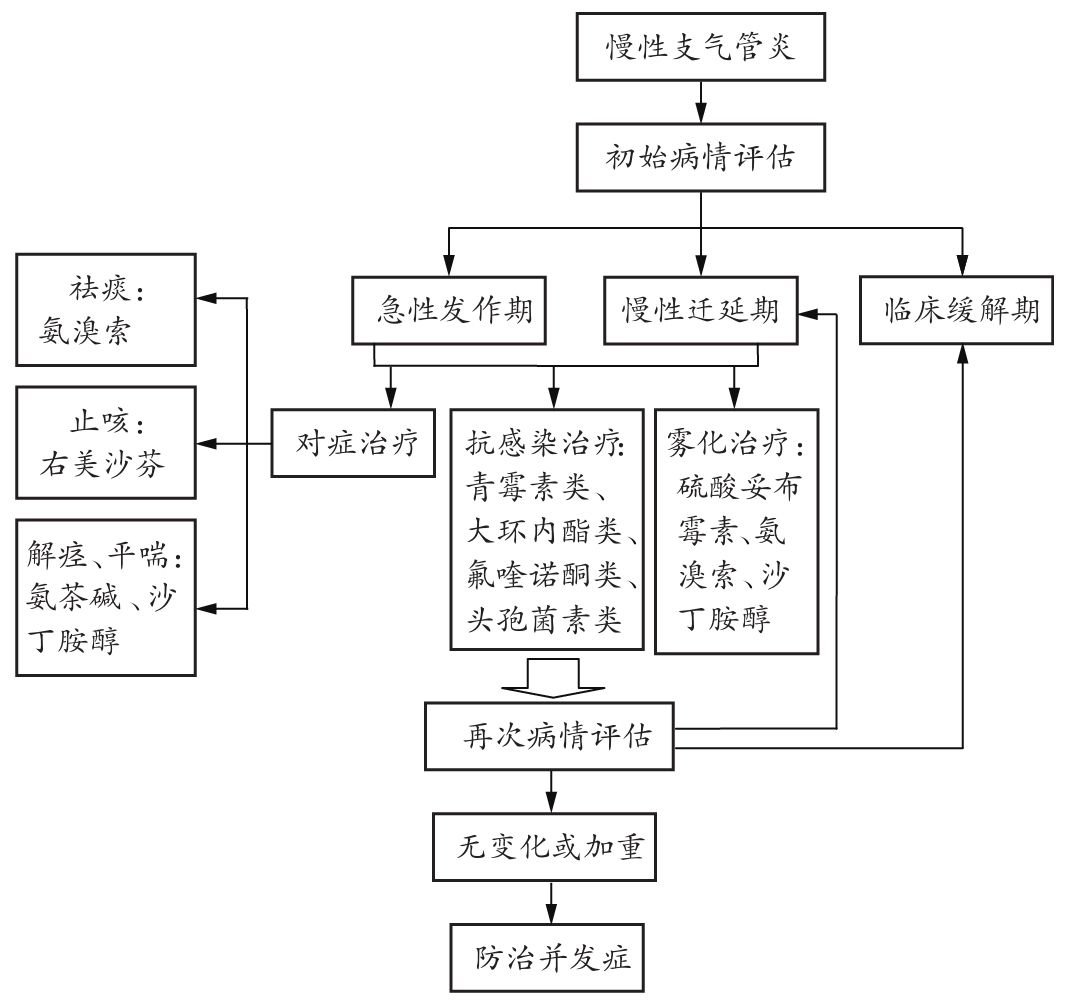
\includegraphics{./images/Image00002.jpg}
 \captionsetup{justification=centering}
 \caption{慢性支气管炎的治疗程序}
 \label{fig1-3-1}
  \end{figure} 

【治疗方案】

{(一)一般治疗}  注意休息、保暖,多饮水,注意加强排痰。

{(二)药物治疗}

1. 急性发作期和慢性迁延期的治疗

(1)控制感染:开始时一般根据临床经验和本地区病原菌耐药性流行病学检测结果选用抗生素,同时积极进行痰病原菌培养和药敏试验。轻者可口服,较重者可用肌注或静脉滴注抗生素,常用有青霉素类、大环内酯类、氨基糖苷类、氟喹诺酮类和头孢菌素类等抗生素。如阿奇霉素0.5g口服,每日1次,或者左氧氟沙星0.5g口服或静脉注射,每日1次。

(2)祛痰、止咳:保持体液平衡可以使痰液变稀薄,有利于粘痰排出。常用祛痰药有溴己新、乙酰半胱氨酸、盐酸氨溴索和标准桃金娘油等,如标准桃金娘油0.3g口服,每日3次。可酌情应用右美沙芬、咳必清或苯丙哌林等镇咳剂,如咳必清25mg口服,每日3次。

(3)解痉、平喘:对于喘息型慢支,常选用解痉平喘药。具体见本书慢性阻塞性肺疾病章节。

(4)雾化治疗:可选用抗生素、祛痰药、解痉平喘药等进行雾化吸入治疗,以加强局部抗炎及稀释痰液作用,喘息型慢支可加用糖皮质激素雾化吸入。如庆大霉素8万U、盐酸氨溴索15ml、沙丁胺醇2ml、异丙托溴铵2ml、布地奈德2ml等的单用或联用,每日2\textasciitilde{}3次射流雾化吸入。

2.
临床缓解期的治疗 可采用气管炎疫苗、卡介菌多糖核酸注射液治疗,冬病夏治以及中药治疗亦可能有一定效果。

【疗效观察与随访】

1. 观察指标

(1)症状、体征:观察咳嗽、咳痰的缓解情况,痰量、痰液性状,以及胸闷、气急的程度。监测体温、两肺呼吸音以及啰音的变化等。

(2)血常规:可根据血象变化,决定下一步治疗方案。

(3)病原学检查:痰涂片、痰培养及药敏试验,有助于指导治疗。

2.
疗效评估 好转标准:症状、体征明显改善,无并发症,相关检查基本正常,但仍时有发作。

3.
随访 注意病情观察,观察症状、体征等变化,避免致病因素,避免合并症、并发症。

【治疗经验与解析】

1.
本病的诊断主要依据临床症状做出诊断。根据咳嗽、咳痰或伴喘息,每年发病持续3个月,连续2年以上,并且排除其他心肺疾患(如肺结核、尘肺、支气管哮喘、支气管扩张症、肺癌、肺脓肿、心功能不全等)之后,即可做出慢支诊断。如每年发病持续时间虽不足3个月,但有明确的客观检查依据(如X线检查),亦可诊断。目前临床上较为常见的问题是过分关注咳嗽、咳痰或喘息症状及持续时间,而忽略了鉴别诊断,导致长期误诊和误治。例如,不少咳嗽变异性哮喘(CVA)被长期按照本病治疗(给予抗生素和各种镇咳药)而疗效不佳,贻误了病情,浪费了医疗资源。

注意:本病的诊断属排他性诊断,做出诊断前必须首先排除其他可以引起慢性咳嗽、咳痰或喘息的心肺疾患,包括肺结核、间质性肺疾病、支气管哮喘、支气管扩张症、肺癌、肺脓肿、心功能不全等。

2.
根据临床特点,本病可分为单纯型和喘息型两种类型。这两种类型的区别主要在于前者仅有咳嗽和咳痰症状,而后者伴有喘息症状和哮鸣音。有学者认为喘息型慢支实际上是本病合并支气管哮喘。

3. 应根据本病的临床分期给予不同的治疗方案。

(1)急性发作期,是指在1周内出现脓性或粘液性痰,痰量明显增加,或伴有发热、白细胞计数增高等炎症表现,或1周内咳嗽、咳痰、喘息中任何一项症状明显加剧。根据喘息、痰量增多和脓性痰等临床表现,具备3项中的任意1项为轻度急性发作,具备3项中的任意2项为中度急性发作,具备全部3项为重度急性发作。对于该期患者应以控制感染和祛痰、止咳为主;伴发喘息时,应同时予解痉平喘治疗。对老年体弱无力咳痰者或痰量较多者,应以祛痰为主,不宜选用强镇咳药,如可待因等,以免抑制呼吸中枢及加重呼吸道阻塞,导致排痰困难、感染加重、病情恶化。

(2)慢性迁延期,是指有不同程度的咳嗽、咳痰或喘息症状迁延不愈1个月以上者。治疗方法基本与急性发作期相同。

(3)临床缓解期,是指咳、痰和气喘症状基本消失,仅偶有轻微咳嗽和少量咳痰,并保持2个月以上者。应注意避免各种致病因素,吸烟者需要戒烟。适度运动。注射流感疫苗和肺炎球菌疫苗可减少本病的发作次数和严重程度。中成药金水宝、补肾防喘片等也可服用。

\section{慢性阻塞性肺疾病}

慢性阻塞性肺疾病(chronic obstructive pulmonary
disease,简称COPD、慢阻肺)是一种具有气流受限特征的可以预防和治疗的疾病,气流受限不完全可逆、呈进行性发展,与肺部对香烟烟雾等有害气体或有害颗粒的异常炎症反应有关。COPD主要累及肺脏,但也可引起全身(或称肺外)的不良效应。COPD起病缓慢,病程较长。一般均有慢性咳嗽、咳痰等慢支症状,但也有少数虽有明显气流受限,却无咳嗽症状。COPD的标志性症状是气短或呼吸困难,从不动不喘、动辄气喘到不动也喘。部分重度患者除了喘息和胸闷外,也可出现体重下降、食欲减退、外周肌肉萎缩、精神抑郁或焦虑等全身症状。合并感染时可咳血痰或咯血。早期体征不明显,随疾病进展可出现肺气肿征、肺部干湿啰音或剑突下心音增强等体征。

【治疗程序】

{(一)COPD急性加重期治疗程序}  图\ref{fig1-4-1}\footnote{ICS:吸入型糖皮质激素 SABA:短效β{2} 受体激动剂}所示。

\begin{figure}[!htbp]
 \centering
 
\includegraphics{./images/Image00003.jpg}
 \captionsetup{justification=centering}
 \caption{COPD急性加重期治疗程序}
 \label{fig1-4-1}
  \end{figure} 


{(二)COPD稳定期治疗程序}  图\ref{fig1-4-2}所示。

\begin{figure}[!htbp]
 \centering
 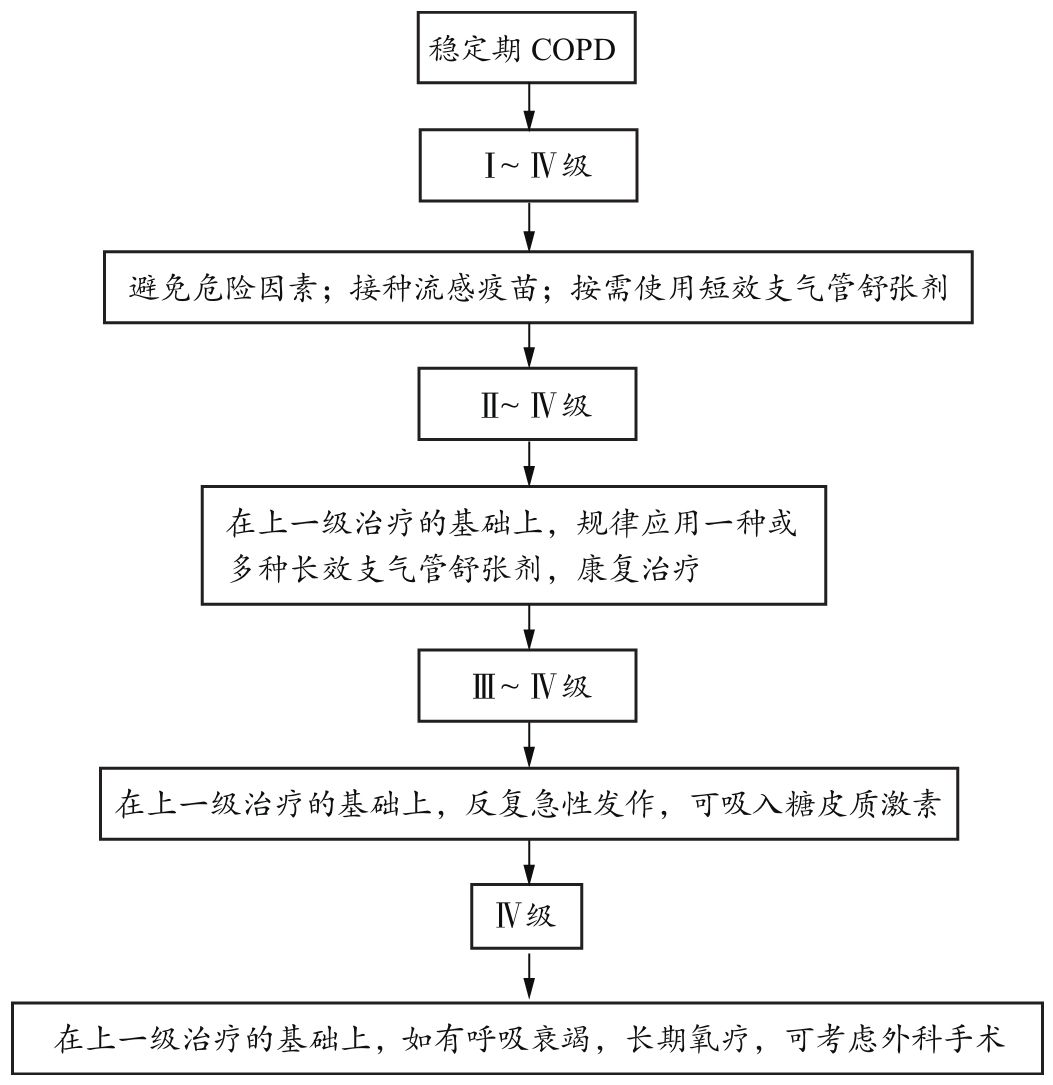
\includegraphics{./images/Image00004.jpg}
 \captionsetup{justification=centering}
 \caption{COPD稳定期的治疗程序}
 \label{fig1-4-2}
  \end{figure} 

【治疗方案】

{(一)一般治疗}
 戒烟,避免或防止粉尘、烟雾及有害气体吸入,进行有规律的体育活动。

{(二)药物及相关治疗}

1. COPD急性加重期(AECOPD)的治疗

(1)控制性氧疗:给氧途径包括鼻导管或文丘里(Venturi)面罩,一般吸入氧浓度28\%\textasciitilde{}30\%。对于住院或急诊ICU患者,氧疗30分钟后应复查动脉血气。血氧饱和度目标值是88\%\textasciitilde{}92\%。

(2)支气管舒张剂:增加支气管舒张剂的剂量及频度,如沙丁胺醇2500μg吸入;联合β{2}
受体激动剂和抗胆碱能药物,如沙丁胺醇1000μg加异丙托溴铵250μg吸入;吸入使用储雾罐或气压雾化器;如果需要,可考虑静脉茶碱治疗,有条件者应监测茶碱血药浓度。

(3)全身应用糖皮质激素:全身激素能缩短康复时间、改进肺功能(FEV{1}
)和动脉血氧分压(PaO{2}
),并降低早起复发风险、减少治疗失败的概率和缩短住院时间。建议每日口服泼尼松30\textasciitilde{}40mg,使用10\textasciitilde{}14日。

(4)控制感染:使用抗生素控制感染的指征:①有以下三种重要症状:呼吸困难加重、咳痰增加、脓痰增加;②患者脓痰增加,同时还有一种其他重要症状;③需要机械辅助通气。结合当地常见致病菌类型及耐药趋势和药敏情况尽早选择敏感抗生素。如对初始治疗方案反应欠佳,应及时根据细菌培养及药敏试验结果调整抗生素。Ⅰ\textasciitilde{}Ⅳ级稳定期COPD的急性加重的致病微生物以及所选抗生素治疗,见表\ref{tab1-4-1}。长期应用广谱抗生素和激素易继发深部真菌感染,应密切观察真菌感染的临床征象并采用防治真菌感染的措施。

\begin{longtable}[]{p{4cm}p{5cm}p{6cm}}
  \caption{AECOPD住院患者抗生素的应用}
  \label{tab1-4-1}\\
\toprule
分级 & 病原微生物 & 抗生素\tabularnewline
\midrule
\endhead
Ⅰ\textasciitilde{}Ⅱ级COPD急性加重 &
流感嗜血杆菌、肺炎链球菌、卡他莫拉菌等 &
青霉素、β内酰胺/酶抑制剂(阿莫西林/克拉维酸)、大环内酯类(阿奇霉素、克拉霉素、罗红霉素等)、第1代或第2代头孢菌素(头孢呋辛、头孢克洛)、多西环素、左氧氟沙星等,一般可口服\tabularnewline
Ⅲ\textasciitilde{}Ⅳ级COPD急性加重(无铜绿假单胞菌感染危险因素) &
流感嗜血杆菌、肺炎链球菌、卡他莫拉菌、肺炎克雷伯菌、大肠杆菌、肠杆菌属等
&
β内酰胺/酶抑制剂、第2代头孢菌素(头孢呋辛)、氟喹诺酮类(左氧氟沙星、莫西沙星、加替沙星)、第3代头孢菌素(头孢曲松、头孢噻肟)等\tabularnewline
Ⅲ\textasciitilde{}Ⅳ级COPD急性加重(有铜绿假单胞菌感染危险因素) &
以上细菌及铜绿假单胞菌 &
第3代头孢菌素(头孢他啶)、头孢哌酮/舒巴坦、呱拉西林/他唑巴坦、亚胺培南、美罗培南等,也可联合氨基糖苷类、氟喹诺酮类(环丙沙星,大剂量左氧氟沙星)\tabularnewline
\bottomrule
\end{longtable}

(5)机械通气:根据病情,可选用无创机械通气或有创机械通气。

(6)其他治疗措施:在出入量和血电解质监测下适当补充液体和电解质;注意维持液体和电解质平衡;注意补充营养,对不能进食者需经胃肠补充要素饮食或予静脉高营养;对卧床、红细胞增多症或脱水的患者,无论是否有血栓栓塞性疾病史,均需考虑使用肝素或低分子肝素;注意痰液引流,积极排痰治疗(如刺激咳嗽,叩击胸部,体位引流等方法);识别并治疗伴随疾病(冠心病、糖尿病、高血压等)及合并症(休克、弥散性血管内凝血、上消化道出血等)。

2. COPD稳定期的治疗

(1)支气管舒张剂:抗胆碱药、β{2}
受体激动剂是COPD常用的制剂,如长效抗胆碱药(LAMA)噻托溴铵18μg吸入,每日1次,或者短效抗胆碱药(SAMA)异丙托溴铵40\textasciitilde{}80μg吸入,每日3\textasciitilde{}4次,或者沙丁胺醇气雾剂100\textasciitilde{}200μg吸入,每24小时不超过12喷。也可用氨茶碱0.1g,每日3次,需注意剂量不能过大,避免不良反应。

(2)糖皮质激素:CODP稳定期长期应用激素吸入治疗并不能阻止其FEV1的降低趋势。长期规律的吸入激素联合β{2}
受体激动剂较适用于FEV1占预计值百分比\textless{}60\%的COPD患者。这一治疗可以改善症状、肺功能和生活质量,降低急性加重的频率。对COPD患者不推荐长期口服激素治疗。

(3)联合吸入激素/支气管扩张剂治疗:联合吸入激素和长效β{2}
受体激动剂(LABA),比各自单用效果好,如沙美特罗替卡松粉吸入剂(舒利迭)50μg/500μg,每日2次,每次1吸。

(4)其他药物:①祛痰药:似有利于气道引流通畅,改善通气,但除少数有粘痰患者获效外,总的来讲效果并不十分确切。常用药物有盐酸氨溴索、乙酰半胱氨酸等,如盐酸氨溴索每次30mg,每日3次。②抗氧化剂:应用抗氧化剂如N-乙酰半胱氨酸可降低疾病反复加重的频率。但目前尚缺乏长期、多中心临床研究结果,有待今后进行严格的临床研究考证。③免疫调节剂:对降低COPD急性加重严重程度可能具有一定的作用。但尚未得到确证,不推荐作常规使用。④疫苗:流感疫苗可降低COPD患者的严重程度,减少死亡,可每年给予1次(秋季)或2次(秋季、冬季)。肺炎球菌疫苗含有23种肺炎球菌荚膜多糖,已在COPD患者中应用,但尚缺乏有力的临床观察资料。⑤磷脂二酯酶-4(PDE-4)抑制剂:对于伴有急性加重史和慢性支气管炎的GOLD3级和4级患者,PDE-4抑制剂罗氟司特与口服激素或长效支气管扩张剂联用时可减少急性加重。⑥中医治疗:辨证施治是中医治疗的原则,对COPD的治疗亦应据此原则进行。实践中体验到某些中药具有祛痰、支气管舒张、免疫调节等作用,值得深入的研究。

(5)氧疗:COPD稳定期进行长期氧疗对具有慢性呼吸衰竭的患者可提高生存率。长期氧疗的指征:①PaO{2}
≤7.3kPa(55mmHg)或SaO{2}
≤88\%,合并或不合并3周内发生2次高碳酸血症;②PaO{2}
在7.3\textasciitilde{}8.0kPa(55\textasciitilde{}60mmHg)之间,或SaO{2}
为88\%,若有证据表明存在肺动脉高压,或提示充血性心力衰竭的外周水肿,或红细胞增多症(红细胞压积\textgreater{}55\%)。一般是经鼻导管吸入氧气,流量1.0\textasciitilde{}2.0升/分,吸氧持续时间\textgreater{}15小时/日。长期氧疗的目的是使患者在海平面水平,静息状态下,达到PaO{2}
≥60mmHg和(或)使SaO{2}
升至90\%,这样才可维持重要器官的功能,保证周围组织的氧供。

(6)辅助通气治疗:联合无创通气和长期氧疗可能对一部分患者有用,特别是明显的日间高碳酸血症患者。连续气道正压通气(CPAP)在改善生存率和降低住院风险方面有明确的益处。

(7)康复治疗:可以使进行性气流受限、严重呼吸困难而很少活动的患者改善活动能力、提高生活质量,是COPD患者一项重要的治疗措施。它包括呼吸生理治疗,肌肉训练,营养支持、精神治疗与教育等多方面措施。在呼吸生理治疗方面包括帮助患者咳嗽,用力呼气以促进分泌物清除;使患者放松,进行缩唇呼吸以及避免快速浅表的呼吸以帮助克服急性呼吸困难等措施。在肌肉训练方面有全身性运动与呼吸肌锻炼,前者包括步行、登楼梯、踏车等,后者有腹式呼吸锻炼等。在营养支持方面,应要求达到理想的体重;同时避免过高碳水化合物饮食和过高热卡摄入,以免产生过多的CO{2}
。

(8)外科治疗:根据病情,可采用肺大疱切除术、肺减容术和肺移植术等。

【疗效观察与随访】

1. 观察指标

(1)症状、体征:观察咳嗽、咳痰和气喘的变化,注意痰液的性状和痰量,注意监测体温。如出现发绀、头痛、嗜睡和神志恍惚等症状,应警惕呼吸衰竭的发生。注意肺部体征,有无干、湿啰音。如剑突下出现心脏搏动及心音增强,提示并发早期肺源性心脏病。

(2)肺功能检查:肺功能测定指标是诊断COPD的金标准,是判断气流受限的客观指标,其重复性好,对COPD的诊断、严重程度评价、疾病进展、预后及治疗反应等均有重要意义。气流受限是以FEV{1}
和FEV{1} /FVC比值降低来确定的。FEV{1}
/FVC比值是COPD的一项敏感指标,可检出轻度气流受限。FEV{1}
占预计值百分比是中、重度气流受限的良好指标,它变异性小,易于操作,应作为COPD肺功能检查的基本项目。吸入支气管舒张剂后(FEV{1}
/FVC)×100\%\textless{}70\%者,可确定为不完全可逆的气流受限。

(3)胸部X线检查:COPD早期胸片可无异常变化,以后出现肺纹理增多、紊乱等非特征性改变;主要X线征为肺过度充气:肺容积增大,胸腔前后径增长,肋骨走向变平,肺野透亮度增高,横幅位置低平,心脏悬垂狭长,肺门血管纹理呈残根状,肺野外周血管纹理纤细稀少等,有时可见肺大疱形成。并发肺动脉高压和肺源性心脏病时,除有右心增大的X线征象外,还可有肺动脉圆锥膨隆,肺门血管影扩大及右下肺动脉增宽等。

(4)血气分析:当FEV{1}
占预计值百分比\textless{}40\%,或呼吸衰竭,或右心衰竭的COPD患者均应做血气分析。血气分析异常首先表现为轻、中度低氧血症。随疾病进展,低氧血症逐渐加重,并出现高碳酸血症。

(5)其他实验室检查:COPD合并细菌感染时,血白细胞增高,核左移。并发感染时痰涂片可见大量中性粒细胞,痰培养可检出各种病原菌,常见者为肺炎链球菌、流感嗜血杆菌、卡他莫拉菌、肺炎克雷伯菌等。

2.
疗效评估 根治痊愈。好转标准:呼吸道感染控制,气促症状减轻,肺功能改善,病情稳定半年以上。

3.
随访 注意病情观察,观察症状、体征等变化,避免致病因素,避免合并症、并发症,并进行COPD评估。评估COPD的目的是决定疾病严重程度,包括COPD对患者健康状况的影响和未来的风险程度(例如急性加重、住院或死亡),最终目的是指导治疗,应基于症状、气流受限程度(行肺功能检查)、急性加重风险、合并症四方面分别进行评估。

(1)COPD的一般评估:

①症状评估:采用COPD评估测试(CAT)或改良英国MRC呼吸困难指数(mMRC)。

②肺功能检查评估气流受限程度:根据气流受限程度对COPD进行分级(见表\ref{tab1-4-2})。

\begin{longtable}[]{lc}
  \caption{COPD患者气流受限分级(吸入支气管舒张剂后)}
  \label{tab1-4-2}\\
\toprule
COPD气流受限分级 & 肺功能特征\tabularnewline
\midrule
\endhead
GOLD 1(轻度) & (FEV{1} /FVC)×100\%\textless{}70\%,FEV{1}
占预计值百分比≥80\%\tabularnewline
GOLD 2(中度) & (FEV{1} /FVC)×100\%\textless{}70\%,50\%≤FEV{1}
占预计值百分比\textless{}80\%\tabularnewline
GOLD 3(重度) & (FEV{1} /FVC)×100\%\textless{}70\%,30\%≤FEV{1}
占预计值百分比\textless{}50\%\tabularnewline
GOLD 4(极重度) & (FEV{1} /FVC)×100\%\textless{}70\%,FEV{1}
占预计值百分比\textless{}30\%\tabularnewline
\bottomrule
\end{longtable}

③急性加重风险的评估:COPD的急性加重是指一种急性起病的过程,其特征是患者呼吸系统症状恶化,超出日常的变异,并且导致需要改变药物治疗。频繁急性加重(每年≥2次)的最佳预测因素是既往急性加重治疗史。当气流受限恶化时,急性加重的风险也相应增加。

④合并症评估:COPD患者常伴有合并症,包括心血管疾病、骨质疏松症、抑郁和焦虑、骨骼肌肉异常、代谢综合征和肺癌等。这些合并症可能影响患者的住院和死亡风险,在诊疗常规中应重视这些合并症,给予适当诊疗。

(2)COPD的综合评估:图\ref{fig1-4-3}提供了这些项目的综合评估,从而达到改善COPD的疾病管理的目的。

\begin{figure}[!htbp]
 \centering
 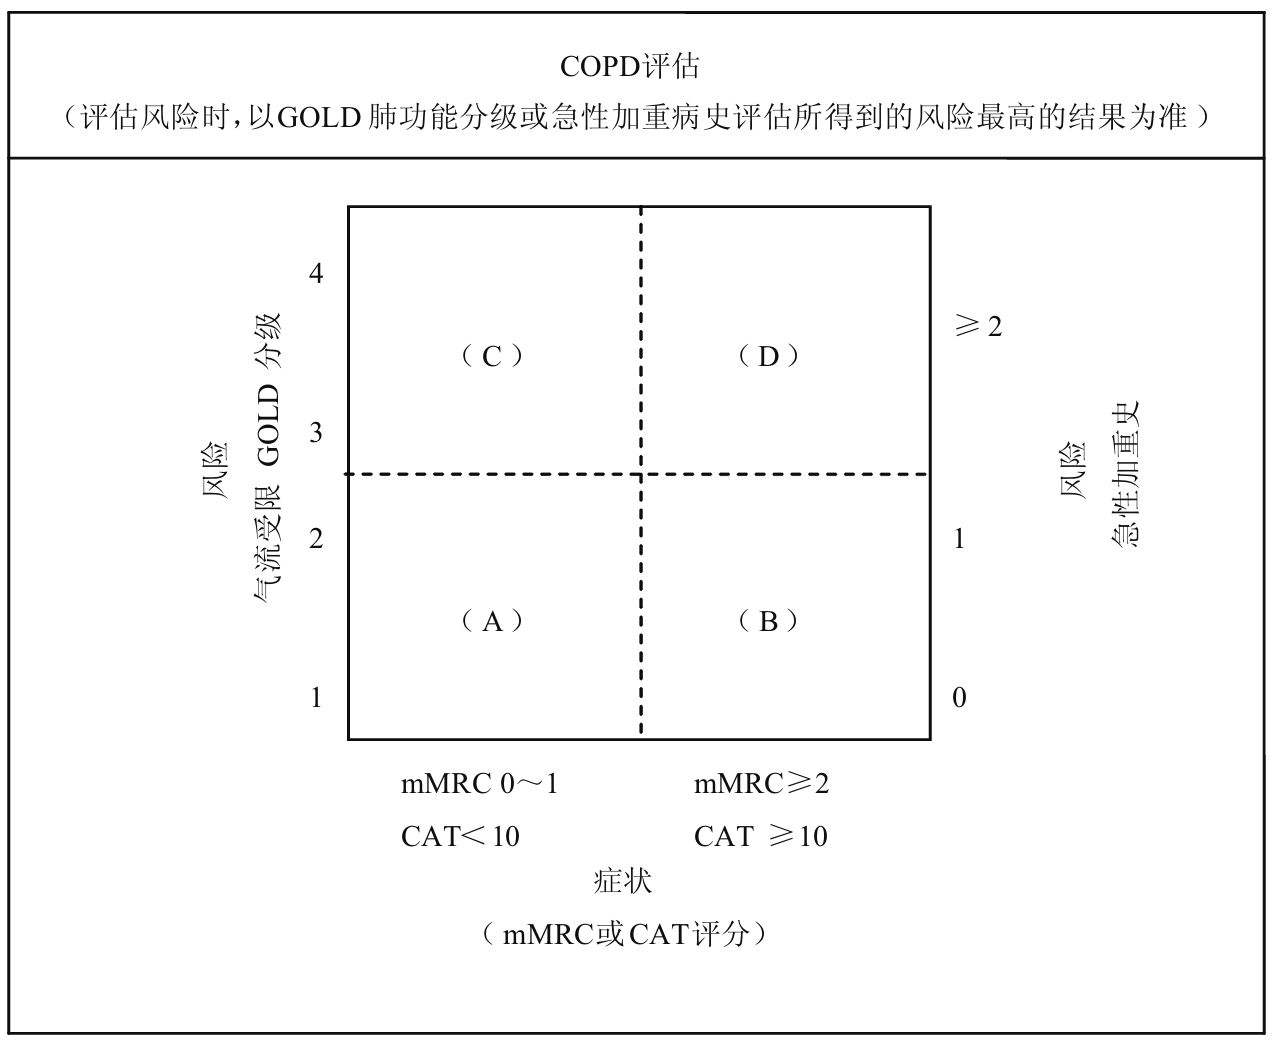
\includegraphics{./images/Image00005.jpg}
 \captionsetup{justification=centering}
 \caption{COPD评估}
 \label{fig1-4-3}
  \end{figure} 

①症状:症状少(mMRC0\textasciitilde{}1或CAT\textless{}10):患者处于A区或C区;症状多(mMRC≥2或CAT≥10):患者处于B区或D区。

②气流受限:低风险(GOLD 1或2):患者处于A区或B区;高风险(GOLD
3或4):患者处于C区或D区。

③急性加重:低风险(每年≤1次):患者处于A区或B区:高风险(每年≥2次):患者处于C区或D区。

【治疗经验与解析】

1.
COPD的教育与管理 通过教育与管理可以提高患者及有关人员对COPD的认识和自身处理疾病的能力,更好地配合治疗和加强预防措施,减少反复加重,维持病情稳定,提高生活质量。主要内容包括:①教育与督促患者戒烟,迄今能证明有效延缓肺功能进行性下降的措施仅有戒烟。一次简短(3分钟)的咨询能使戒烟率达到5\%\textasciitilde{}10\%。尼古丁替代治疗亦能提高长期戒烟率。②使患者了解COPD的病理生理与临床基础知识。③掌握一般和某些特殊的治疗方法。④学会自我控制病情的技巧,如进行腹式呼吸及缩唇呼吸锻炼等。⑤了解赴医院就诊的时机。⑥社区医生定期随访管理。

2.
支气管扩张剂治疗 首选吸入治疗。短期按需应用支气管扩张剂可缓解症状,长期规则应用可预防和减轻症状。较之短效制剂,吸入长效支气管扩张剂更为方便,而且效果较好。与增加一种支气管扩张剂剂量相比,联合应用多种支气管扩张剂可以增加疗效、减少不良反应。一般不建议使用茶碱。

3.
COPD稳定期的药物治疗 A组首选SAMA必要时或SABA必要时,第二选择LAMA或LABA或SAMA和SABA,其他备选可有茶碱;B组首选LAMA或LABA,第二选择LAMA和LABA,其他备选可有SABA和(或)SAMA、茶碱;C组首选ICS/LABA或LAMA,第二选择LAMA和LABA,LAMA和PDE-4抑制剂,或LABA和PDE-4抑制剂,其他备选可有SABA和(或)SAMA、茶碱;D组首选ICS/LABA和(或)LABA,第二选择ICS+LABA和LAMA,或ICS/LABA和PDE-4抑制剂,或LAMA+LABA,或LAMA和PDE-4抑制剂,其他备选可有羧甲司坦、SABA和(或)SAMA、茶碱。

4.
ICS/LABA治疗 TORCH研究显示,沙美特罗替卡松粉吸入剂(舒利迭)50μg/500μg可以显著降低COPD急性加重的发生率、降低患者的死亡风险,并可显著改善患者肺功能、提高呼吸能力,明显提高患者的生活质量。在3年的研究中,舒利迭50μg/500μg组与安慰剂组的死亡率分别为12.6\%和15.2\%,联合治疗较安慰剂的死亡率降低了17.5\%,但P=0.052。两组的差异无统计学意义的原因可能因设计的样本量偏小,导致检验效力不足。也可能因安慰剂组退出试验的患者较多,退出试验的主要原因是急性加重,而这部分急性加重的患者又正是死亡风险高的患者。假设他们没有退出,安慰剂组的死亡率可能更高而达到有统计学意义的差异。所以,舒利迭治疗能否降低COPD死亡率目前尚无明确的答案。

\section{慢性肺源性心脏病}

慢性肺源性心脏病(chroniccorpulmonale,简称慢性肺心病)是由于慢性支气管肺疾病、胸廓疾病、肺血管疾病或呼吸调节功能障碍引起肺循环阻力增加、肺动脉高压,进而引起右心室肥厚、扩大,甚至发生右心功能衰竭的心脏病。由先天性心脏病和左心疾病引起的右心室肥厚、扩大或右心功能衰竭不属于肺心病。临床上除了原有肺、胸疾病的各种症状和体征外,主要是逐步出现的肺、心功能不全以及其他器官受损的征象。

【治疗程序】 图\ref{fig1-5-1}所示。

\begin{figure}[!htbp]
 \centering
 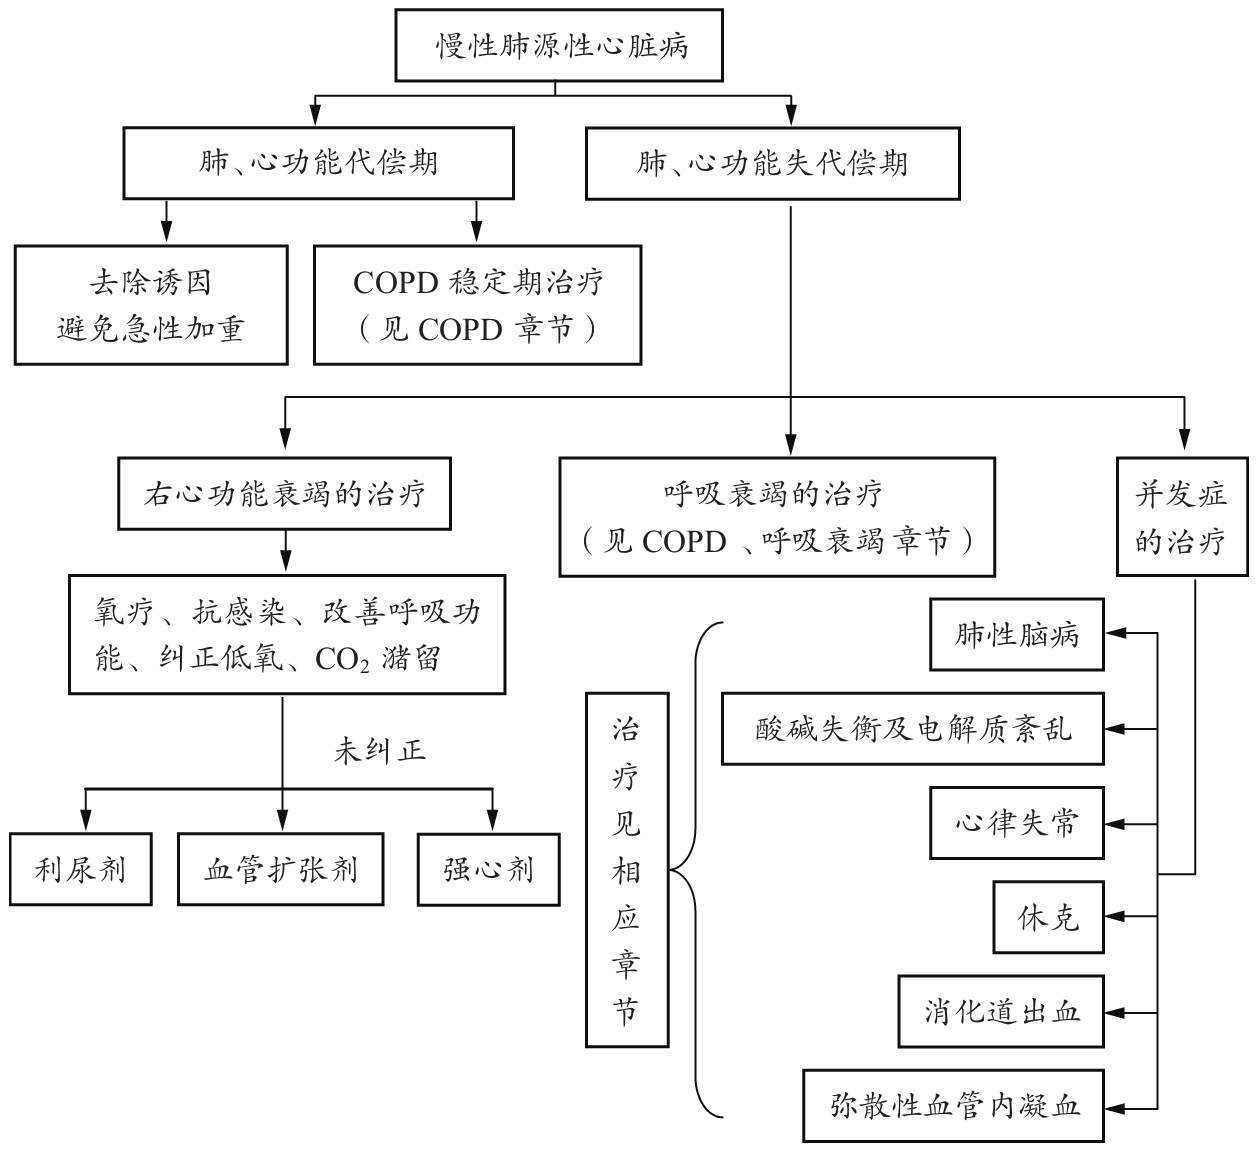
\includegraphics{./images/Image00006.jpg}
 \captionsetup{justification=centering}
 \caption{慢性肺源性心脏病的治疗程序}
 \label{fig1-5-1}
  \end{figure} 

【治疗方案】

{(一)一般治疗}  戒烟,避免或防止粉尘、烟雾及有害气体吸入。

{(二)药物及相关治疗}

1.
肺、心功能代偿期 ①采用中西医结合的综合措施,增强患者的免疫功能。②去除诱因,避免急性加重。③继发于COPD者,治疗参见COPD章节。

2. 肺、心功能失代偿期

(1)呼吸衰竭的治疗:抗感染,使用支气管舒张剂和祛痰药,吸痰,保持呼吸道通畅,纠正缺氧和CO{2}
潴留等,具体参见COPD、呼吸衰竭章节。

(2)右心功能衰竭的治疗:一般经过氧疗、抗感染、改善呼吸功能、纠正低氧、CO{2}
潴留后,心力衰竭症状可减轻或消失,患者尿量增多,水肿消退,肿大的肝缩小、压痛消失,不需常规使用利尿剂和强心剂。病情较重或上述治疗无效者,可酌情选用利尿剂和强心剂,如氢氯噻嗪25mg,每日1\textasciitilde{}3次,联合螺内酯40mg,每日1\textasciitilde{}2次。重症急需利尿者,可用呋塞米20mg肌注或口服。也可用毛花苷C(西地兰)0.2\textasciitilde{}0.4mg加入葡萄糖液20ml内缓慢静脉注射。应用血管扩张剂治疗有效,如硝酸甘油、酚妥拉明、硝苯地平、卡托普利和依拉普利等。近来发现,吸入NO有效,吸入浓度一般为20\textasciitilde{}40ppm。

(3)并发症的治疗:肺性脑病、酸碱失衡及电解质紊乱、心律失常、休克、消化道出血以及弥散性血管内凝血的治疗,具体参见本书相应章节。

【疗效观察与随访】

1. 观察指标

(1)症状、体征:

①肺、心功能代偿期:表现肺胸基础疾病的症状,如COPD患者可有咳嗽、咳痰、气促,活动后可有心悸、呼吸困难、乏力和劳动耐力下降。急性感染可使上述症状加重。除可见肺胸疾病的体征外,尚可见肺动脉高压和右室扩大的体征,如P{2}
\textgreater{}A{2}
,三尖瓣区出现收缩期杂音,剑突下心脏搏动增强,部分可有颈静脉充盈。

②肺、心功能失代偿期:a.呼吸衰竭详见本书呼吸衰竭章节,可表现为呼吸困难加重,夜间为甚,常有头痛、失眠、食欲下降,但白天嗜睡,甚至出现表情淡漠、神志恍惚和谵妄等肺性脑病的表现。除了有明显发绀外,可出现球结膜充血、水肿,严重时可有视网膜血管扩张、视盘水肿等颅内压升高的表现。腱反射减弱或消失,出现病理反射。也可有皮肤潮红、多汗。b.右心功能衰竭时除肺胸疾患的症状更明显外,尚可有心悸、食欲不振、腹胀、恶心等右心功能衰竭的表现。表现为发绀更明显,颈静脉怒张,心率增快,可出现心律失常,剑突下可闻及收缩期杂音,甚至出现舒张期杂音。肝大且有压痛,肝颈静脉回流征阳性,下肢水肿,重者可有腹腔积液。

(2)X线检查:除有肺、胸基础疾病及急性肺部感染的体征外,尚有肺动脉高压征。其X线诊断标准如下:①右下肺动脉干扩张,横径≥15mm或右下肺动脉横径与气管横径比值≥1.07,或经动态观察右下肺动脉干增宽2mm以上;②肺动脉段中度突出或其高度≥3mm;③中心肺动脉扩张和外周分支纤细两者形成鲜明对比;④圆锥部显著突出(右前斜位45°)或其高度≥7mm;⑤右心室增多。具有上述五项中的一项可以诊断。

(3)心电图检查:心电图对肺心病的阳性率为60.1\%\textasciitilde{}88.2\%。典型慢性肺心病的心电图可见电轴右偏,顺时针方向转位,肺型P波,V{1}
导联QRS波呈qR,V{5} R/S\textless{}1,R{v1} +S{v5} \textgreater{}1.05mV。

(4)超声心动图检查:诊断符合率为60.6\%\textasciitilde{}87\%,较心电图和X线检查的敏感性高。慢性肺心病超声心动图改变表现为如右室流出道内径≥30mm,右心室内径≥20mm,右心室前壁厚度≥5mm或有前壁搏动幅度增强,右肺动脉内径≥18mm或肺动脉干≥20mm等。

(5)血气分析:用以判断有无缺氧、CO{2}
潴留和酸碱平衡紊乱及其严重程度,对于指导肺心病急性发作期的治疗具有重要意义。

(6)血液检查:血常规检查可见有无红细胞增多症和感染,血电解质测定可了解有无电解质紊乱,凝血功能检查有助于了解有无血液高凝状态等。

2.
疗效评估 好转标准:心衰纠正,呼吸稍平稳,发绀消失,呼吸道感染控制,咳痰仍较多,活动后仍心悸。几乎无法治愈。

3.
随访 注意病情观察,观察症状、体征等变化,避免致病因素,避免并发症。定期复查心电图、血气分析、胸部X线摄片、血象等。

【治疗经验与解析】

1.
右心功能衰竭利尿剂的应用 利尿剂通过抑制肾脏钠、水重吸收而增加尿量,消除水肿,减少循环血容量,减轻右心前负荷,纠正右心功能衰竭。但利尿剂使用过多、利尿过猛对慢性肺心病患者也有不利的一面,大量利尿后可以使痰液变粘稠,不易咳出,可导致电解质紊乱,致使血液粘滞性进一步升高。因此,使用原则是小剂量、联合使用排钾和保钾利尿剂,疗程宜短,间歇用药。

2.
右心功能衰竭强心剂的应用 因慢性肺心病缺氧而使心脏对洋地黄的敏感性增高,因此使用洋地黄应慎重。在下列情况下仍应考虑使用洋地黄:感染已控制,呼吸功能已改善,经利尿剂治疗右心功能仍未改善者;合并室上性心律失常,如室上性心动过速、快速心房颤动者;以右心功能衰竭为主要表现而无明显急性感染的患者;合并急性左心功能衰竭者。使用原则是选用作用快、排泄快的强心剂,小剂量(常规剂量的1/3至1/2)给药。

3.
右心功能衰竭血管扩张剂的应用 血管扩张剂可使肺动脉扩张,降低肺动脉高压,以减轻右心负荷,改善右心功能。但许多血管扩张剂会同时引起体循环动脉血压下降,导致冠状动脉血流减少等不良反应。此外,肺血管扩张后常有影响肺内通气/血流的比例,加重低氧血症。因此在使用时应掌握适当的剂量,密切监测病情变化。同时可适当使用支气管扩张剂以改善肺泡通气功能。

\section{支气管哮喘}

支气管哮喘(bronchial
asthma,简称哮喘)是由多种炎症细胞(如嗜酸性粒细胞、肥大细胞、T淋巴细胞、中性粒细胞等)、结构细胞(如平滑肌细胞、气道上皮细胞等)和细胞组分参与的常见气道慢性炎症性疾病。全球约有3亿哮喘患者。典型哮喘的诊断依据包括:①反复发作喘息、气急、胸闷或咳嗽,多与接触变应原、冷空气、物理、化学性刺激、病毒性上呼吸道感染、运动等有关。②发作时在双肺可闻及散在或弥漫性、以呼气相为主的哮鸣音,呼气相延长。③上述症状可经治疗缓解或自行缓解。④除外其他疾病所引起的喘息、气急、胸闷和咳嗽。临床表现不典型(如无明显喘息或体征,以顽固性咳嗽或胸闷为主要症状)的哮喘,至少应有下列3项肺功能试验中的一项:①支气管激发试验或运动试验阳性;②支气管舒张试验阳性,FEV{1}
增加≥12\%,且FEV{1}
增加绝对值≥200ml;③呼气流量峰值(PEF)日内(或2周)变异率≥20\%,并除外其他疾病时才能作出支气管哮喘的诊断。根据临床表现,哮喘可分为急性发作期、慢性持续期和临床缓解期。

【治疗程序】

{(一)慢性哮喘患者的管理程序}  图\ref{fig1-6-1}所示。

\begin{figure}[!htbp]
 \centering
 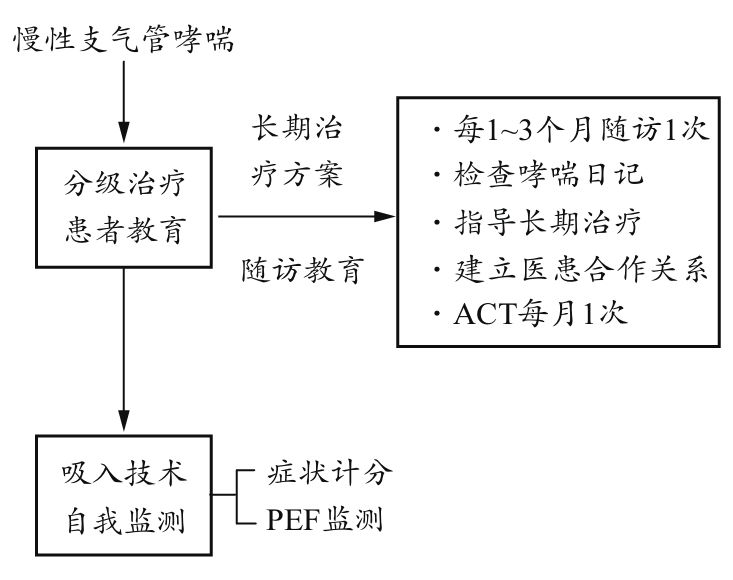
\includegraphics{./images/Image00007.jpg}
 \captionsetup{justification=centering}
 \caption{慢性哮喘患者的管理程序}
 \label{fig1-6-1}
  \end{figure} 

{(二)哮喘急性发作期治疗方案}  图\ref{fig1-6-2}\footnote{SABA:短效β{2} 受体激动剂}所示。

\begin{figure}[!htbp]
 \centering
 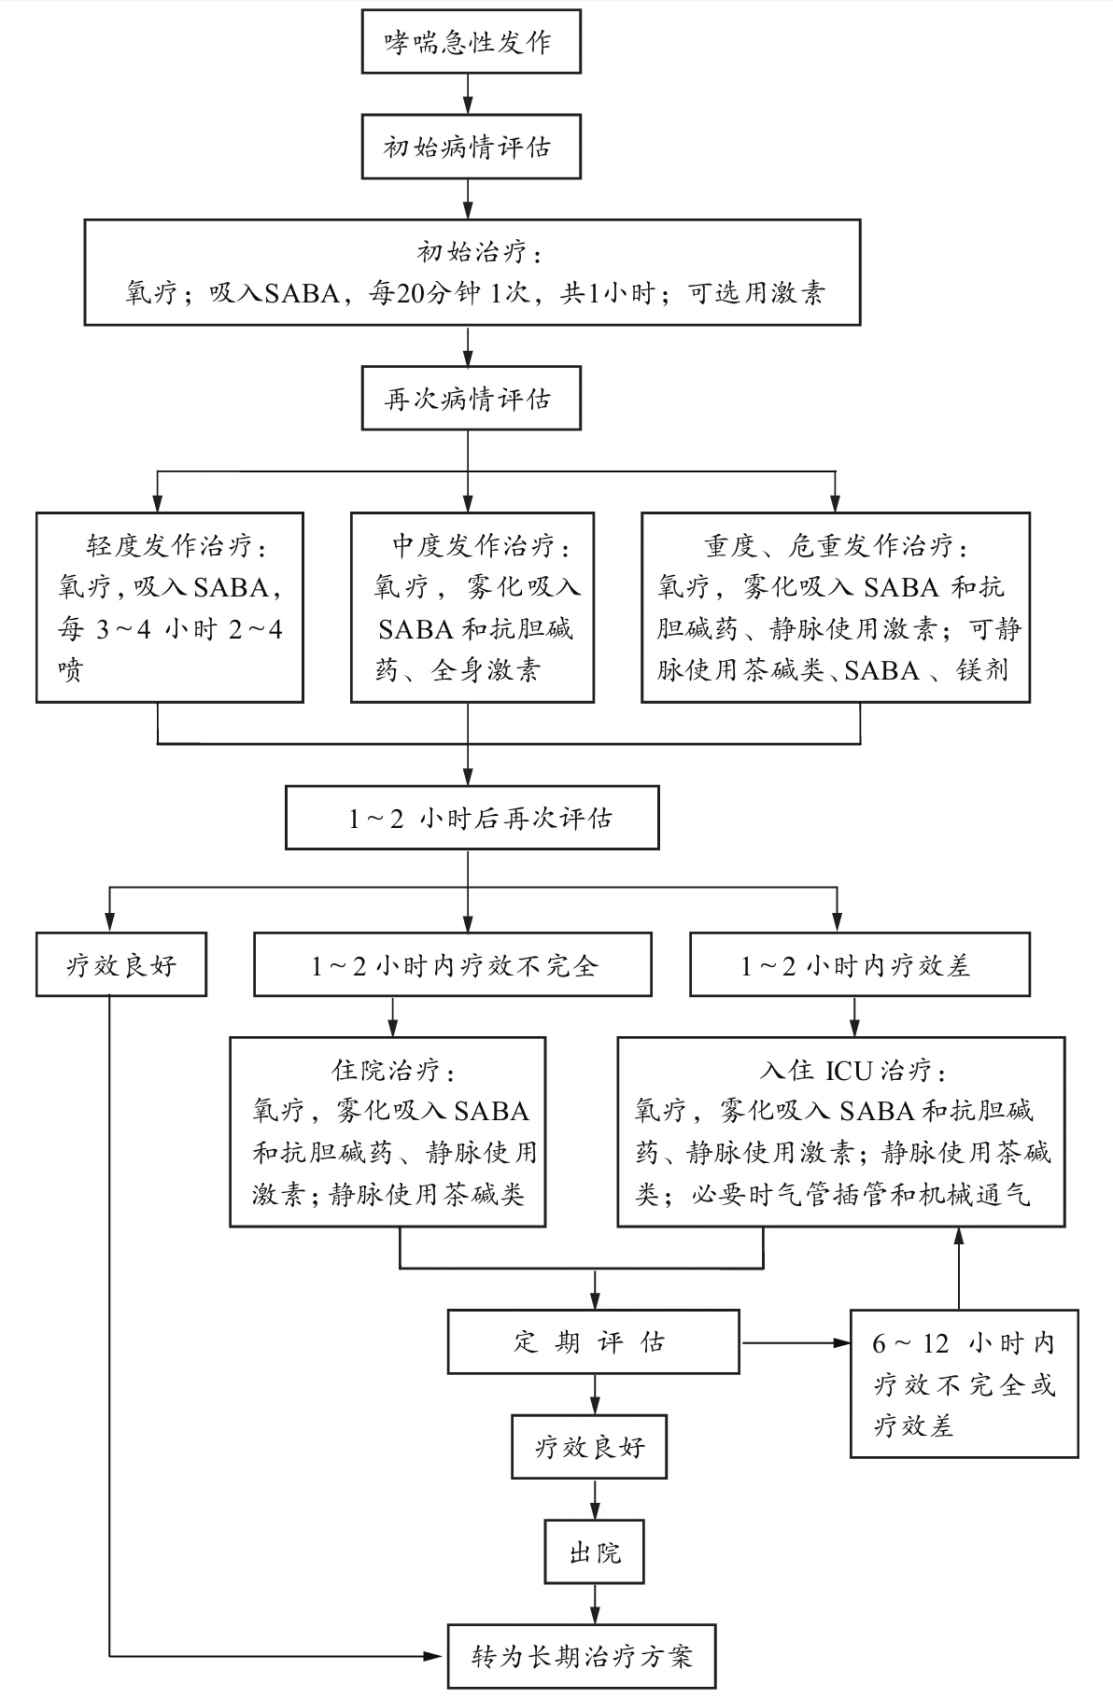
\includegraphics{./images/Image00008.jpg}
 \captionsetup{justification=centering}
 \caption{哮喘急性发作的治疗程序}
 \label{fig1-6-2}
  \end{figure} 

{(三)哮喘长期治疗程序}  图\ref{fig1-6-3}\footnote{ICS:吸入型糖皮质激素 LABA:长效β{2} 受体激动剂}所示。

\begin{figure}[!htbp]
 \centering
 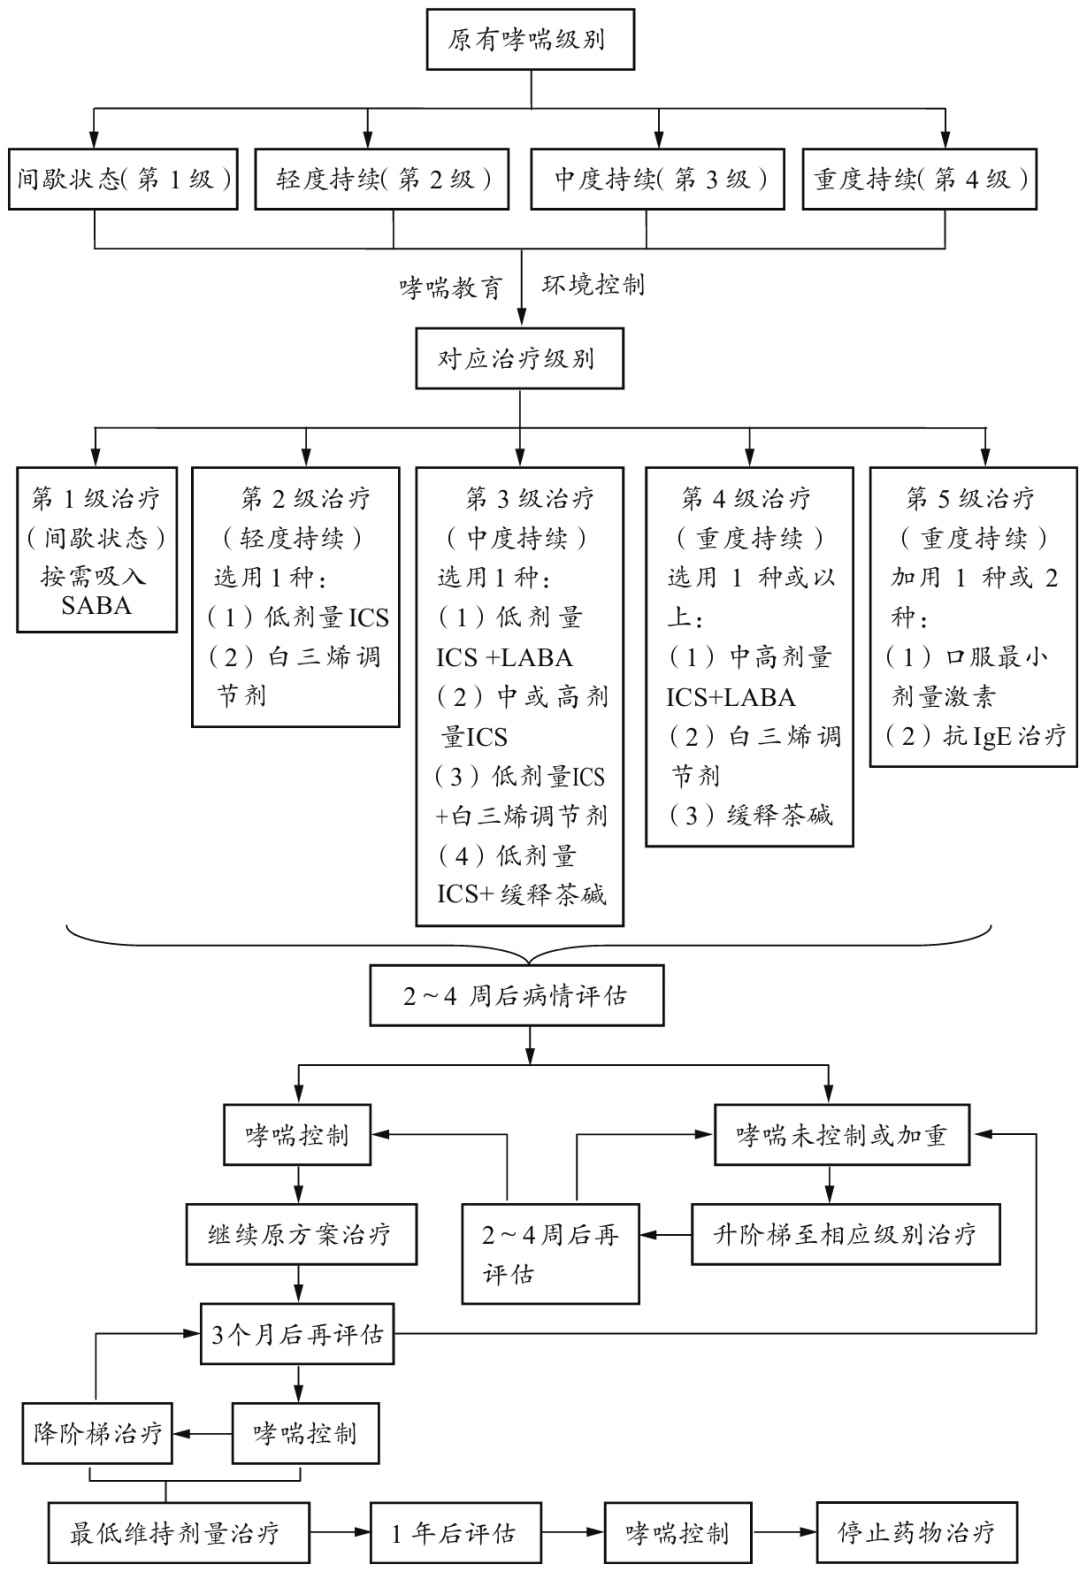
\includegraphics{./images/Image00009.jpg}
 \captionsetup{justification=centering}
 \caption{哮喘长期治疗程序}
 \label{fig1-6-3}
  \end{figure} 

	

【治疗方案】

{(一)一般治疗}

1.
治疗目标 哮喘的治疗目标:①达到并维持症状的控制。②维持正常活动,包括运动能力。③维持肺功能水平尽量接近正常。④预防哮喘急性加重。⑤避免因哮喘药物治疗导致的不良反应。⑥预防哮喘导致的死亡。

2.
预防措施 应尽可能避免或减少接触危险因素,包括变应原、病毒感染、污染物和烟草烟雾等,预防哮喘发病和症状加重。

{(二)药物治疗}

1. 常用治疗哮喘药物 可以分为控制药物和缓解药物两大类。

(1)控制药物:是指需要长期每日使用的药物。包括全身用糖皮质激素(简称激素)、吸入型糖皮质激素(ICS)、白三烯调节剂、长效β{2}
受体激动剂(LABA,须与ICS联合应用)、缓释茶碱、色苷酸钠、抗IgE抗体等。

(2)缓解药物:是指按需使用缓解喘息症状的药物。包括吸入速效β{2}
受体激动剂、全身用激素、吸入性抗胆碱药物、短效茶碱及口服短效β{2}
受体激动剂等。

2. 哮喘急性发作期治疗

(1)轻度和部分中度急性发作:治疗措施主要为重复吸入SABA和吸氧。如吸入沙丁胺醇(如万托林)气雾剂,在第1小时内每20分钟吸入2\textasciitilde{}4喷。随后根据治疗反应,轻度急性发作可调整为每3\textasciitilde{}4小时2\textasciitilde{}4喷,中度急性发作每1\textasciitilde{}2小时6\textasciitilde{}10喷。如果对SABA反应良好(呼吸困难显著缓解,PEF占预计值\textgreater{}80\%或个人最佳值,且疗效维持3\textasciitilde{}4小时),通常不需要使用其他药物。如果治疗反应不完全,尤其是在控制性治疗的基础上发生的急性发作,应尽早口服激素(泼尼松龙0.5\textasciitilde{}1mg/kg或等效剂量的其他激素),必要时去医院就诊。

(2)中度以上急性发作:部分中度和所有重度急性发作的患者均应去医院治疗。除氧疗外,应重复使用SABA。在初始治疗时间段(每20分钟)或连续雾化给药,随后根据需要间断给药(每4小时1次)。联合吸入SABA和抗胆碱药物(异丙托溴铵)能够取得更好的支气管舒张作用。氨茶碱每小时0.6\textasciitilde{}0.8mg/kg静脉滴注,可以维持有效血药浓度,从而扩张支气管。如果24小时内患者未用过茶碱,则应首先缓慢地经静脉注射负荷量(4\textasciitilde{}6mg/kg)的氨茶碱,以使茶碱迅速达到有效血浓度,注射时间应大于20分钟。应该尽早使用全身激素,特别是对SABA初始治疗反应不完全或疗效不能维持,以及在口服激素基础上仍然出现急性发作的患者。推荐用法:泼尼松龙每日30\textasciitilde{}50mg或等效的其他激素,分1\textasciitilde{}2次口服。

(3)重度和危重度哮喘发作:除了上述治疗措施外,尚应酌情给予下列治疗:①静脉注射或滴注激素:如甲泼尼龙40\textasciitilde{}80mg,或氢化可的松10mg/(kg·d)分次给药。②补液:纠正因哮喘持续发作时张口呼吸、出汗、进食少等原因引起的脱水,可避免痰液粘稠导致气道堵塞。根据失水及心脏情况,每日静脉补液量一般为2000\textasciitilde{}2500ml。③纠正酸中毒:严重缺氧可引起代谢性酸中毒,后者可使患者的支气管对平喘药的反应性降低。可用5\%碳酸氢钠静脉滴注或缓慢静脉注射。④抗生素:重度哮喘发作患者气道阻塞严重,易产生呼吸道感染,故应酌情选用广谱抗生素静脉滴注。⑤纠正电解质紊乱:部分患者可因反复应用β{2}
受体激动剂和大量出汗而出现低钾、低钠等电解质紊乱,应及时纠正。⑥并发症的处理及机械通气的应用:并发张力性气胸应及时行胸腔闭式引流术,粘液痰栓阻塞气道可行支气管肺泡灌洗术(BAL)。应及时机械通气治疗,其指征主要包括意识改变、呼吸肌疲劳、PaCO{2}
≥45mmHg等。

3. 哮喘长期治疗方案

(1)第1级治疗:用于哮喘间歇状态(第1级)的治疗。按需吸入SABA,如每次吸入200μg沙丁胺醇气雾剂。

(2)第2级治疗:用于轻度持续(第2级)哮喘的治疗。选用低剂量ICS或白三烯调节剂,如丙酸氟替卡松(辅舒酮气雾剂)100μg,每日2次吸入;或孟鲁司特钠(顺尔宁)10mg,每日1次口服。常用ICS的每日剂量与互换关系见下表(表\ref{tab1-6-1})。


\begin{longtable}[]{@{}llll@{}}
  \caption{常用ICS的每日剂量与互换关系}
  \label{tab1-6-1}\\
\toprule
药 物 & 低剂量(μg) & 中剂量(μg) & 高剂量(μg)\tabularnewline
\midrule
\endhead
二丙酸倍氯米松 & 200\textasciitilde{}500 & 500\textasciitilde{}1000 &
\textgreater{}1000\textasciitilde{}2000\tabularnewline
布地奈德 & 200\textasciitilde{}400 & 400\textasciitilde{}800 &
\textgreater{}800\textasciitilde{}1600\tabularnewline
丙酸氟替卡松 & 100\textasciitilde{}250 & 250\textasciitilde{}500 &
\textgreater{}500\textasciitilde{}1000\tabularnewline
环索奈德 & 80\textasciitilde{}160 & 160\textasciitilde{}320 &
\textgreater{}320\textasciitilde{}1280\tabularnewline
\bottomrule
\end{longtable}

(3)第3级治疗:用于中度持续(第3级)哮喘的治疗。首选低剂量ICS+LABA。也可酌情选用中或高剂量ICS,或低剂量ICS+白三烯调节剂,或低剂量ICS+缓释茶碱。如沙美特罗替卡松粉吸入剂(舒利迭)50μg/100μg,每日2次,每次1吸;或丙酸氟替卡松(辅舒酮气雾剂)250μg,每日2次吸入;或布地奈德(普米克都保)200μg,每日2次吸入,联合孟鲁司特钠(顺尔宁)10mg,每日1次口服;或布地奈德(普米克都保)200μg,每日2次吸入,联合多索茶碱0.2g,每日2次口服。

(4)第4级治疗:用于重度持续(第4级)哮喘的治疗。首选中高剂量ICS+LABA。也可酌情选用中高剂量ICS加白三烯调节剂或缓释茶碱。如沙美特罗替卡松粉吸入剂(舒利迭)50μg/500μg,每日2次,每次1吸;孟鲁司特钠(顺尔宁)10mg,每日1次口服;多索茶碱0.2g,每日2次口服。

(5)第5级治疗:用于经上述治疗不理想的重度持续(第4级)哮喘的治疗。在上述治疗基础上加用口服激素或抗IgE治疗。如加用泼尼松30\textasciitilde{}40mg,每日1次口服,症状控制后逐渐减量。对于血清IgE明显增高的哮喘患者,可加用抗IgE单克隆抗体125\textasciitilde{}375mg,皮下注射,每2\textasciitilde{}4周1次。

【疗效观察与随访】

1.
观察指标 观察治疗后喘息、气急、胸闷和咳嗽的变化,肺部体征的变化,监测PEF日内变异率。检测嗜酸性粒细胞(EOS)计数、血常规、IgE、电解质以及C反应蛋白(CRP)变化,注意监测血氧饱和度以及血气分析,观察患者有无嗜睡,意识模糊,有无张力性气胸等并发症,必要时予胸部X片或胸部CT检查。

(1)哮喘急性发作:是指喘息、气促、咳嗽、胸闷等症状突然发生,或原有症状急剧加重,常有呼吸困难,以呼气流量降低为其特征,常因接触变应原、刺激物或呼吸道感染诱发。其程度轻重不一,病情加重,可在数小时或数日内出现,偶尔可在数分钟内危及生命,故应对病情做出正确评估,以便给予及时有效的紧急治疗。哮喘急性发作的严重程度分为4级(表\ref{tab1-6-2}\footnote{只要有符合某一严重程度的指标,即可提示为该级别的急性发作})。

\begin{table}[!htbp]
  \centering
  \caption{哮喘急性发作严重程度的分级}
  \label{tab1-6-2}
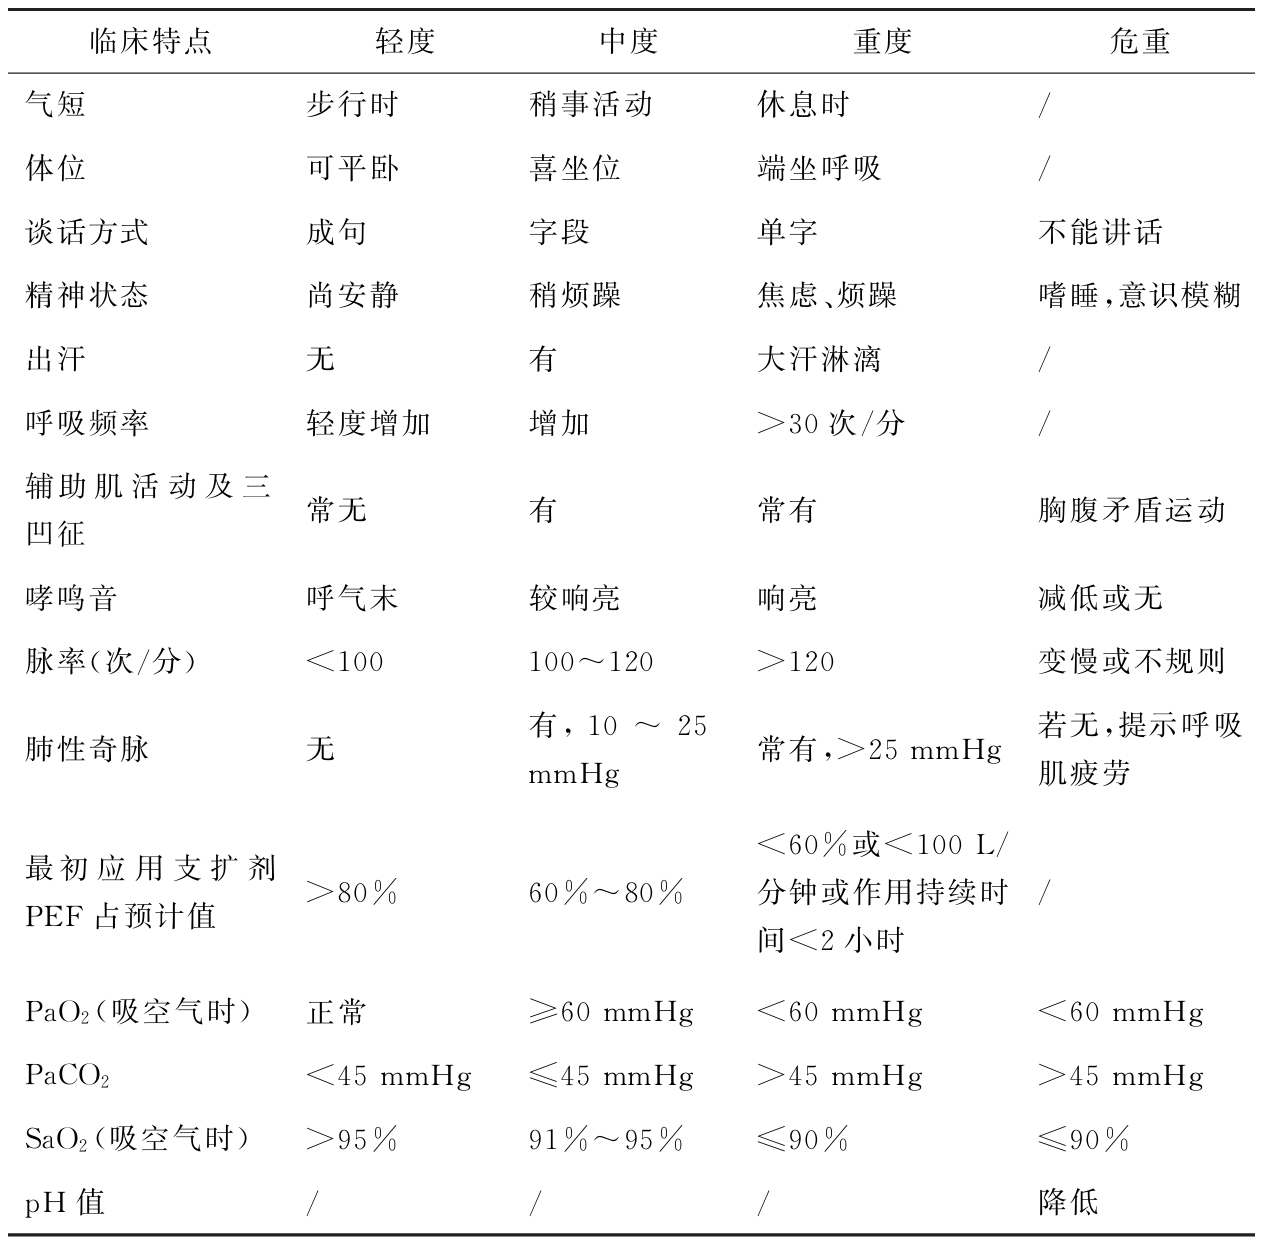
\includegraphics{./images/Image00010.jpg}
\end{table}



①初始病情评估:病史、体检(听诊、辅助呼吸肌活动情况、心率和呼吸频率)、检查结果(PEF或FEV{1}
、血氧饱和度监测、动脉血气分析)。

②再次病情评估:必要时再次体检并检测PEF、血氧饱和度等。

③疗效评估

疗效良好:a.末次治疗后疗效维持1小时。b.体检正常。c.PEF\textgreater{}70\%。d.没有呼吸窘迫。e.氧饱和度\textgreater{}90\%。

1\textasciitilde{}2小时内疗效不完全:a.病史:高危患者(包括曾经有过气管插管和机械通气濒于致死性哮喘的病史;在过去1年中因为哮喘而住院或急诊;正在使用或最近刚停用口服糖皮质激素;目前未使用吸入糖皮质激素;过分依赖SABA,特别是每月使用沙丁胺醇气雾剂或等效药物超过1支;有心理疾病或社会心理问题,包括使用镇静剂;有对哮喘治疗计划不依从的历史)。b.查体:轻至中度体征,即两肺散在低至中调干性啰音,呼气末明显。c.PEF占预计值\%或个人最佳值\textless{}70\%;d.血氧饱和度没有改善。

1小时内疗效差:a.病史:高危患者。b.症状严重,存在嗜睡、意识模糊等,查体示呼吸浅快,胸腹矛盾运动,三凹征,两肺散在高调干性啰音,或者呼吸音减弱或消失(沉默肺)。c.PEF\textless{}30\%预计值。d.PaCO{2}
\textgreater{}45mmHg。e.PaO{2} \textless{}60mmHg。

出院标准:症状缓解,PEF占预计值\%或个人最佳值的60\%,口服或吸入药物即可维持疗效。

(2)哮喘长期治疗:注意根据病情转归,及时给予升级治疗、降级治疗或维持原治疗。

①分级及治疗方案:首先对慢性哮喘患者根据严重程度进行分级,然后根据病情分级制定相应的1\textasciitilde{}4级分级治疗方案。慢性哮喘根据严重程度进行分级,见表\ref{tab1-6-3}\footnote{根据其中最为严重的指标决定分级;PEF变异率(\%)=(最大PEF值-最小PEF值)÷1/2(最大PEF值+最小PEF值)}。

\begin{longtable}[]{lp{5cm}p{5cm}}
  \caption{慢性哮喘的分级}
  \label{tab1-6-3}\\
\toprule
严重程度分级 & 治疗前临床表现 & 肺 功 能\tabularnewline
\midrule
\endhead
间歇状态(第1级) &
每周发作少于1次,两次发作间无症状且PEF正常,夜间症状每月≤2次 & FEV{1}
或PEF\textgreater{}预计值80\%,PEF或FEV{1} 变异率\textless{}20\%,用β{2}
激动剂后正常\tabularnewline
轻度持续(第2级) &
每周哮喘发作2\textasciitilde{}6次,每个月夜间哮喘发作\textgreater{}2次,但\textless{}每周1次
& FEV{1} 或PEF≥预计值80\%,PEF或FEV{1}
变异率20\%\textasciitilde{}30\%\tabularnewline
中度持续(第3级) & 每日发作哮喘,每周夜间哮喘大于1次,每日需使用β{2}
受体激动剂,发作时活动受限 & FEV{1}
或PEF在预计值60\%\textasciitilde{}79\%之间,PEF或FEV{1}
变异率\textgreater{}30\%,治疗后可接近正常\tabularnewline
重度持续(第4级) &
经常持续发作,夜间症状频繁近期有危及生命的大发作,活动受限 & FEV{1}
或PEF\textless{}预计值的60\%,PEF或FEV{1}
变异率\textgreater{}30\%,经积极治疗仍低于正常\tabularnewline
\bottomrule
\end{longtable}


②回访:通常情况下患者在初诊后2\textasciitilde{}4周回访,以后每1\textasciitilde{}3个月随访1次。出现哮喘发作时应及时就诊,哮喘发作后2\textasciitilde{}4周内进行回访。

③如果哮喘未控制或加重:应根据目前哮喘的严重程度,重新制定相应的分级治疗方案。

④各级治疗达到完全控制后:需维持原剂量治疗至少3个月后,然后降级治疗。若分级规范治疗后重新评定病情级别未下降,则应升级治疗,至少维持3个月。

⑤减量方案:单独使用中至高剂量ICS的患者,将ICS剂量减少50\%;单独使用低剂量ICS的患者,可改为每日1次用药;联合ICS和LABA的患者,将ICS剂量减少约50\%,仍继续使用LABA联合治疗。当达到低剂量联合治疗时,可选择改为每日1次联合用药或停用LABA,单用吸入激素治疗。

⑥停止药物治疗标准:经过减量方案后,患者使用最低剂量控制药物达到哮喘控制1年,并且哮喘症状不再发作可考虑停用药物治疗。哮喘控制水平分级见表\ref{tab1-6-4}。


\begin{longtable}[]{lp{3cm}p{3cm}p{3cm}}
  \caption{哮喘控制水平分级}
  \label{tab1-6-4}\\
\toprule\addlinespace[0pt]
\rowcolor{lightgray}&完全控制(满足以下所有条件) & 部分控制(在任何1周内出现以下1\textasciitilde{}2项特征)
&未控制(在任何1周内)\tabularnewline
\midrule
\endhead
白天症状 & 无(或≤2次/周) & \textless{}2次/周 & ---\tabularnewline
\rowcolor{lightgray}活动受限 & 无 & 有 & ---\tabularnewline
夜间症状/憋醒 & 无 & 有 & 出现≥3项部分控制特征\tabularnewline
\rowcolor{lightgray}需要使用缓解药的次数 & 无(或≤2次/周) & \textgreater{}2次/周 &---\tabularnewline
肺功能(PEF或FEV{1} ) & 正常 &
\textless{}正常预计值(或本人最佳值)的80\% & ---\tabularnewline
\rowcolor{lightgray}急性发作 & 无 & ≥每年1次 & 在任何1周内出现1次\tabularnewline
\bottomrule
\end{longtable}

⑦ACT的应用:可用于评估哮喘控制水平。经国内多中心验证表明,ACT不仅易学、易用而且适合中国国情。ACT仅通过回答有关哮喘症状和生活质量5个问题的评分进行综合判定,25分为控制、20\textasciitilde{}24分为部分控制、19分以下为未控制,并不需要患者检查肺功能。ACT内容见表\ref{tab1-6-5}。

\begin{table}[!htbp]
  \centering
  \caption{哮喘控制测试(ACT)表}
  \label{tab1-6-5}
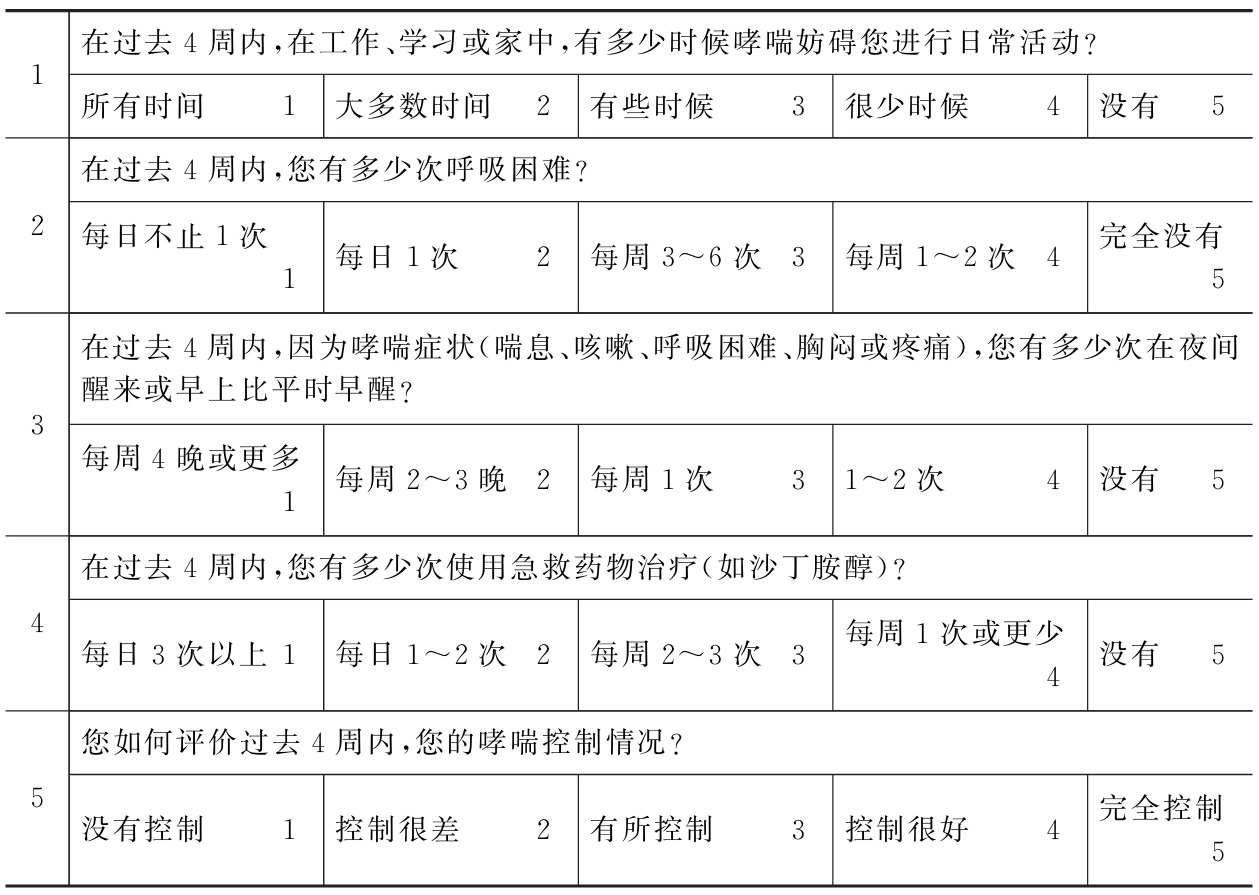
\includegraphics{./images/Image00011.jpg}
\end{table}

2.
随访和患者教育 除了对慢性哮喘患者按时进行随访外,应注重对患者的教育。

(1)教育内容:①通过长期规范治疗能够有效控制哮喘。②避免触发、诱发因素的方法。③哮喘的本质、发病机制。④哮喘长期治疗方法。⑤药物吸入装置及使用方法。⑥自我监测:如何测定、记录、解释哮喘日记内容:症状评分、应用药物、PEF,哮喘控制测试(ACT)变化。⑦哮喘先兆、哮喘发作征象和相应自我处理方法,如何及何时就医。⑧哮喘防治药物知识。⑨如何根据自我监测结果判定控制水平来选择治疗。⑩心理因素在哮喘发病中的作用。

(2)教育方式:包括初诊教育、随访教育和评价、集中教育、自学教育、网络教育、互助学习、定点教育以及调动全社会各阶层力量宣传普及哮喘防治知识。

【治疗经验与解析】

1.
ICS的应用要点 ①ICS是哮喘长期治疗的首选药物。②多数成人哮喘患者吸入小剂量激素即可较好的控制哮喘。由于吸烟可以降低ICS的效果,故吸烟患者须戒烟并给予较高剂量的ICS。③ICS在口咽部局部的不良反应包括声音嘶哑、咽部不适和假丝酵母菌感染。吸药后及时用清水含漱口咽部,选用干粉吸入剂或加用储雾器可减少上述不良反应。④成人哮喘患者每日吸入低、中剂量激素,一般不会出现明显的全身不良反应。长期高剂量吸入糖皮质激素后可能出现的全身不良反应包括皮肤瘀斑、肾上腺功能抑制和骨密度降低等。⑤伴有活动性肺结核的哮喘患者可以在抗结核治疗的同时给予ICS治疗。

2.
吸入疗法由于使用方便,作用直接迅速,局部药物浓度高,疗效好,所用药物剂量小,避免或减少全身用药可能产生的不良反应,因而是治疗哮喘的首选给药途径。①溶液雾化吸入特别适合哮喘急性发作以及年龄小或年龄老、不能很好掌握气雾剂或干粉吸入装置的患者。另外,雾化吸入的药物不含氟利昂等刺激物,不易引起患者呛咳。它吸入肺部药量较高,由于是反复吸入过程,平均5\textasciitilde{}8分钟,因此药物沉积时间长。②射流雾化器产生的雾粒直径适宜(\textless{}5μm),而超声雾化提供的雾粒较大,不易吸入肺部。超声雾化的气雾密度高,可以增加气道阻力,并且由于有些药物可被超声波或加热破坏(激素,蛋白质类),因此应选择射流雾化。③哮喘患者可以雾化吸入的药物包括激素(布地奈德雾化混悬液,即普米克令舒),β{2}
受体激动剂(特布他林溶液,如博利康尼雾化溶液;沙丁胺醇溶液,如万托林雾化溶液),抗胆碱药物(异丙托溴铵溶液,如爱全乐雾化溶液),复合制剂(含有异丙托溴铵和沙丁胺醇的复方异丙托溴铵溶液,如可必特)以及祛痰药(氨溴索针剂,如沐舒坦针剂)等。

3. 中度以上哮喘急性发作的治疗要点 ①目前尚无证据支持常规静脉使用β{2}
受体激动剂。②茶碱类药物虽然价格便宜,但因影响血药浓度的因素多,“治疗窗”窄,应正确使用。静滴的速度过快或剂量过大,可能引起心律失常甚至心搏骤停。对规则服用缓释茶碱的患者,静脉使用茶碱应尽可能监测茶碱血药浓度。

4.
重度和危重度哮喘发作的治疗要点 ①地塞米松因半衰期较长,对肾上腺皮质功能抑制作用较强,一般不推荐使用。②静脉给药和口服给药的序贯疗法有可能减少激素用量和不良反应,如静脉使用激素2\textasciitilde{}3日,继之以口服激素3\textasciitilde{}5日。③不推荐常规使用镁制剂,但可试用于重度急性发作(FEV{1}
25\%\textasciitilde{}30\%)或对初始治疗反应不良者。因硫酸镁对中枢有抑制作用,不宜用于CO{2}
潴留的患者。④补液时应遵循补液的一般原则,即先快后慢、先盐后糖、见尿补钾。纠正酸中毒时,应避免形成碱血症,因为氧离曲线左移不利于血氧在组织中的释放。⑤机械通气时,可先采用经鼻(面)罩无创机械通气,若无效应及早行气管插管机械通气。需要较高的吸气压,可使用适当水平的呼气末正压(PEEP)治疗。如果需要过高的气道峰压和平台压才能维持正常通气容积,可试用允许性高碳酸血症通气策略以减少呼吸机相关性肺损伤。

5.
哮喘长期治疗方案的选择要点 ①以患者的病情严重程度为基础,根据哮喘控制水平类别选择适当的治疗方案。哮喘药物的选择既要考虑疗效及安全性,也要考虑患者的实际状况(如经济收入和当地的医疗资源等)。②对以往未经规范治疗的初诊哮喘患者可选择第2级治疗方案,哮喘患者症状明显,应直接选择第3级治疗方案。从第2\textasciitilde{}5级的治疗方案中都有不同的哮喘控制药物可供选择。而在每一级中都应按需使用缓解药物,以迅速缓解哮喘症状。③近年来推荐联合吸入ICS和LABA治疗哮喘。这两者具有协同的抗炎和平喘作用,可获得相当于(或优于)应用加倍剂量ICS时的疗效,并可增加患者的依从性、减少较大剂量ICS引起的不良反应,尤其适合于中、重度持续哮喘患者的长期治疗。LABA;作为长效支气管扩张药,单独应用可增加发生严重哮喘和死亡的概率,因此不能单独吸入,必须与ICS等哮喘控制药物联合应用。

6. 咳嗽变异性哮喘的诊治要点 咳嗽变异性哮喘(cough variant
asthma,CVA)是以顽固性咳嗽为唯一的临床表现,无喘息症状,故临床上易于被误诊为“支气管炎”等疾病。以下特点有助于诊断:①病史:咳嗽和胸闷症状常呈季节性,部分患者患有其他变态反应疾病(如过敏性鼻炎等)或有家族过敏史。

②肺功能试验:气道反应性测定、支气管激发试验或支气管舒张试验有助于诊断。

③试验性治疗:原先经积极的抗感染和镇咳药物治疗无效,给予平喘和抗过敏治疗后咳嗽和胸闷症状明显缓解,也有助于CVA的诊断。

CVA的治疗应参考典型哮喘的治疗方案,长期应用ICS等药物。

7.
注意合并自发性气胸的可能性 病程长的哮喘患者,由于肺气肿和肺大疱的形成,偶可在哮喘急性发作时并发气胸,使呼吸困难的症状突然加重。如果忽略了并发气胸的可能性,误以为是哮喘发作加剧而反复使用平喘药物,就必将延误治疗。并发气胸的特征是出现胸部重压感,大多为单侧性,吸气性呼吸困难,且平喘药物治疗无效。通过仔细体格检查或者胸部X线检查即可作出及时诊断,关键在于患者和医务人员的重视程度和是否及时检查治疗。

\section{咳嗽}

咳嗽是机体的防御反射,有利于清除呼吸道分泌物和有害因子,但频繁剧烈的咳嗽对患者的工作、生活和社会活动造成严重的影响。临床上,咳嗽是内科患者最常见的症状,咳嗽病因繁多且涉及面广,特别是胸部影像学检查无明显异常的慢性咳嗽患者,此类患者最易被临床医生所疏忽,很多患者被长期误诊为“慢性支气管炎”或“支气管炎”,大量使用抗菌药物治疗而无效,或者因诊断不清反复进行各种检查,不仅增加了患者的痛苦,也加重了患者的经济负担。通常根据时间,将咳嗽分为急性咳嗽(\textless{}3周)、亚急性咳嗽(3\textasciitilde{}8周)和慢性咳嗽(\textgreater{}8周)3类。也可根据X线胸片有无异常,分为2类,本章节重点讨论X线胸片无明显异常,以咳嗽为主要或唯一症状者,即通常所说的不明原因慢性咳嗽(简称慢性咳嗽)。

【治疗程序】

{(一)急性咳嗽的治疗程序}  图\ref{fig1-7-1}所示。

\begin{figure}[!htbp]
 \centering
 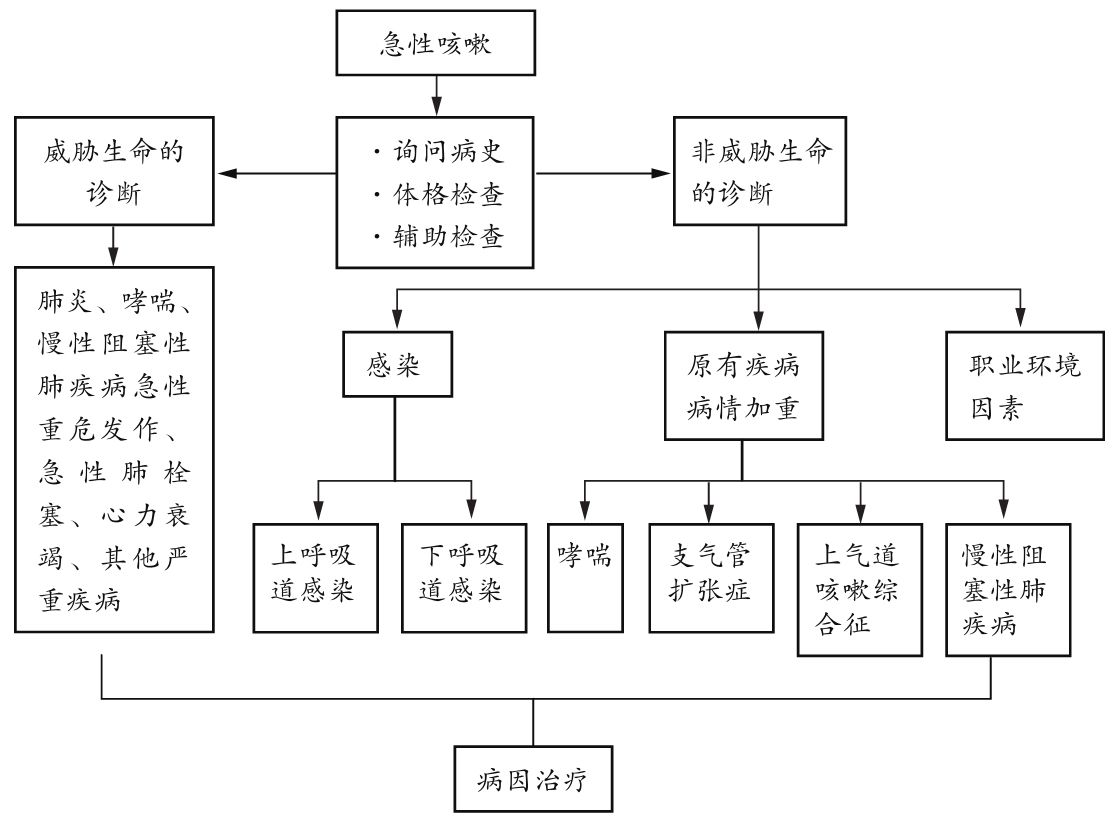
\includegraphics{./images/Image00012.jpg}
 \captionsetup{justification=centering}
 \caption{急性咳嗽的治疗程序}
 \label{fig1-7-1}
  \end{figure} 

{(二)亚急性咳嗽的治疗程序}  图\ref{fig1-7-2}所示。

\begin{figure}[!htbp]
 \centering
 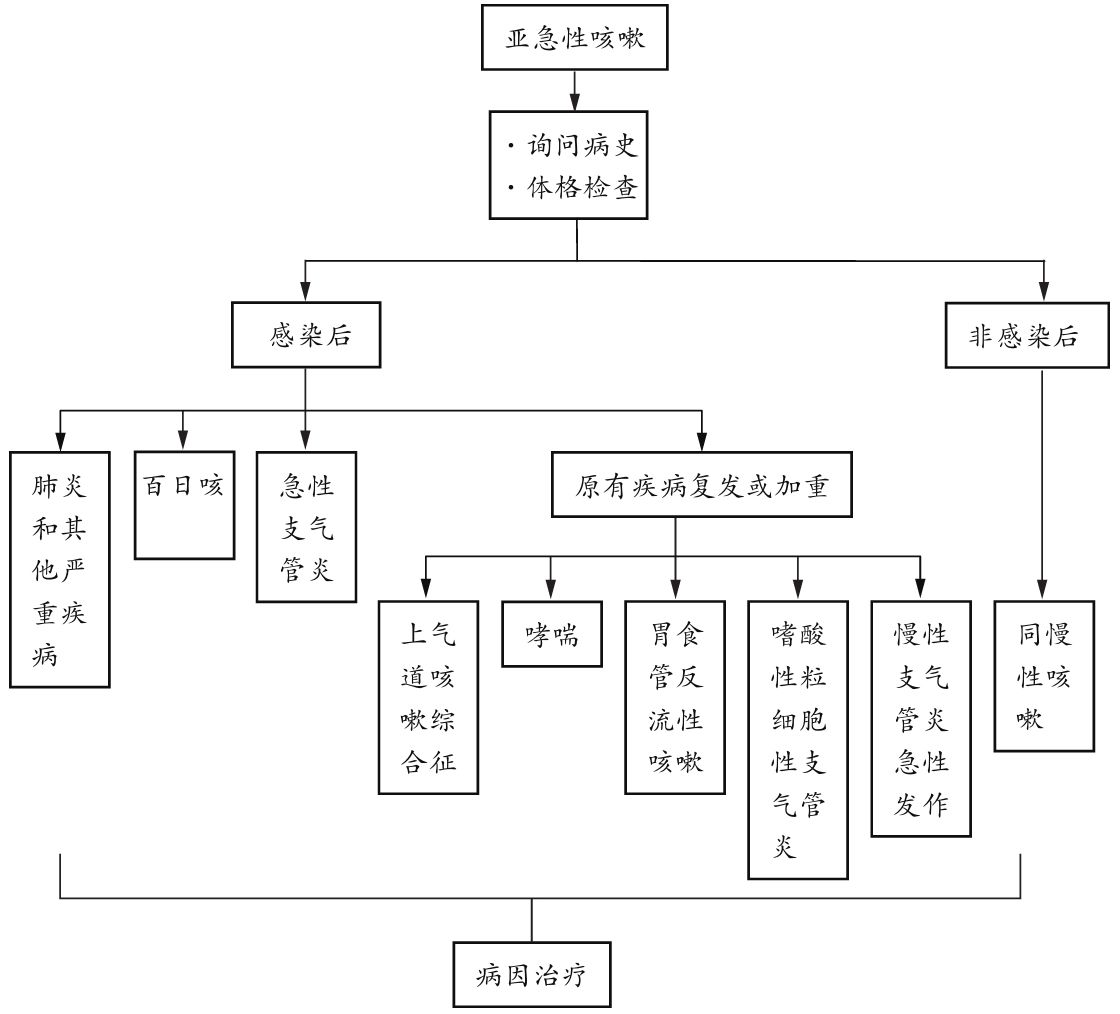
\includegraphics{./images/Image00013.jpg}
 \captionsetup{justification=centering}
 \caption{亚急性咳嗽的治疗程序}
 \label{fig1-7-2}
  \end{figure} 

{(三)慢性咳嗽的治疗程序}  图\ref{fig1-7-3}所示。

\begin{figure}[!htbp]
 \centering
 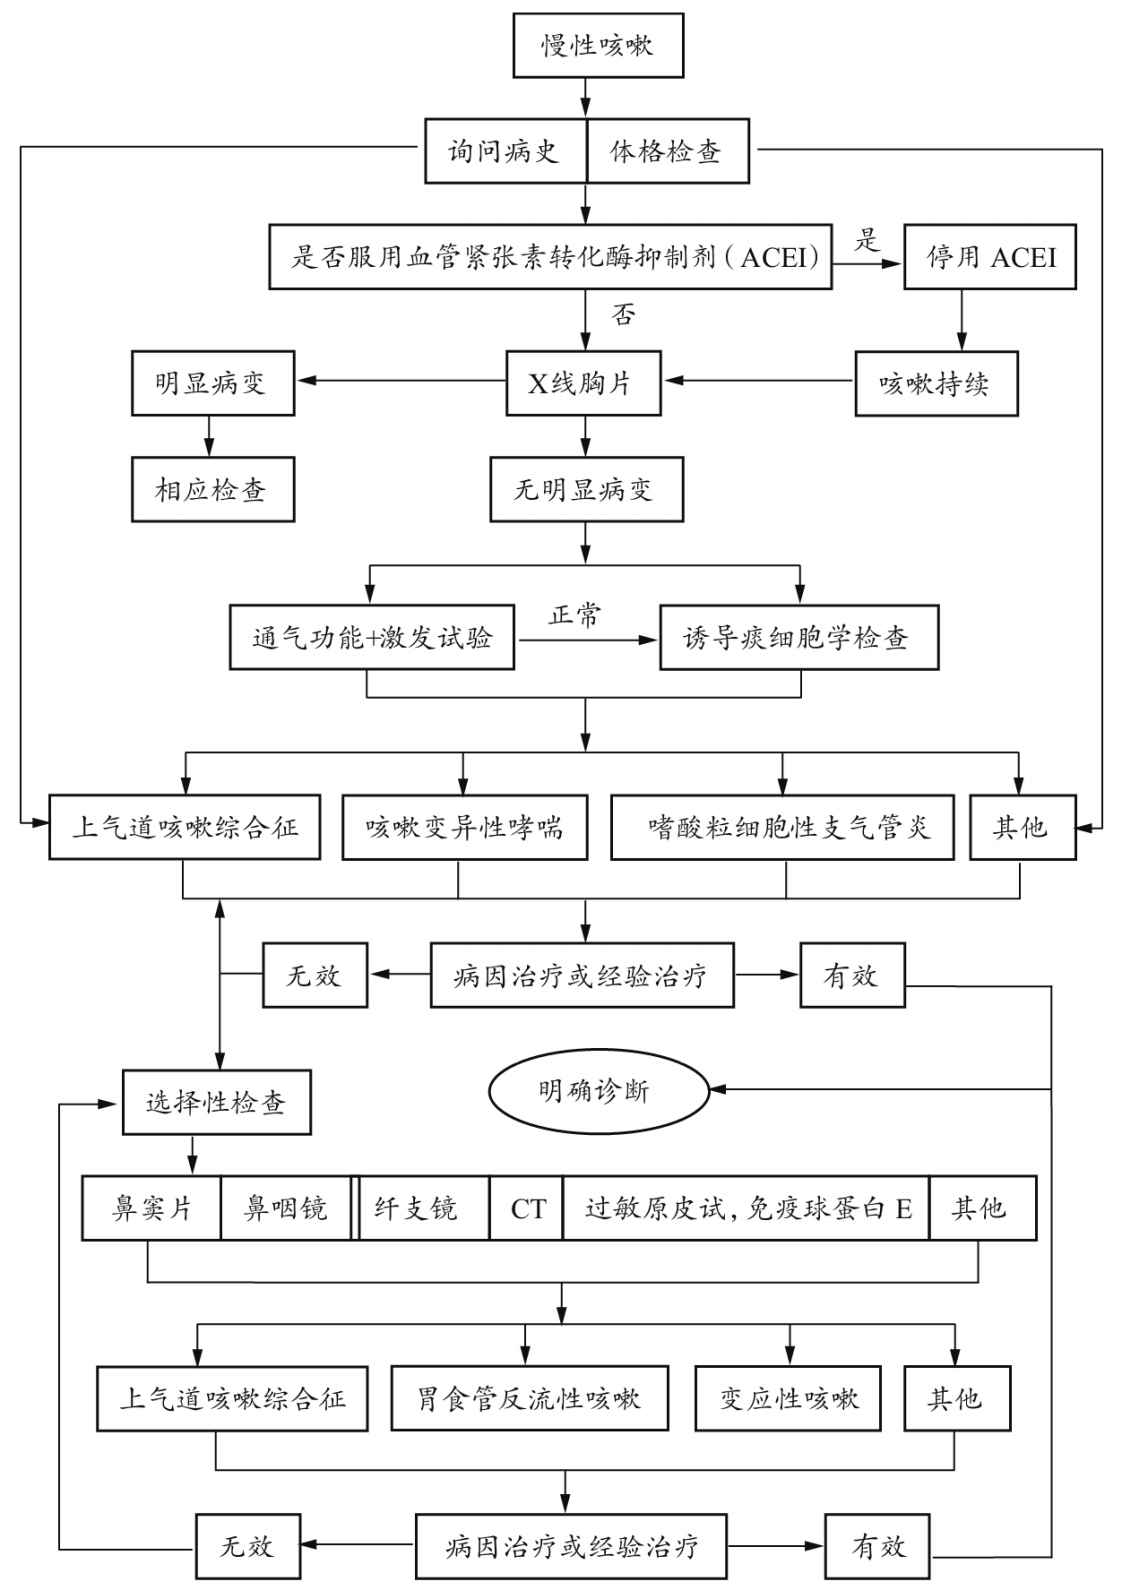
\includegraphics{./images/Image00014.jpg}
 \captionsetup{justification=centering}
 \caption{慢性咳嗽的治疗程序}
 \label{fig1-7-3}
  \end{figure} 

【治疗方案】

{(一)一般治疗}
 积极寻找病因,针对病因治疗,避免诱发因素,适当对症治疗。

{(二)药物治疗}

1. 常用治疗咳嗽药物

(1)镇咳药:如磷酸可待因,每次15\textasciitilde{}30mg口服或皮下注射,每日总量可为30\textasciitilde{}90mg;右美沙芬,每次15\textasciitilde{}30mg口服,每日3\textasciitilde{}4次;苯丙哌林,每次20\textasciitilde{}40mg口服,每日3次。

(2)祛痰药:如愈创甘油醚,每次10\textasciitilde{}20ml口服,每日3次;氨溴索,每次30mg口服,每日3次;溴己新,每次8\textasciitilde{}16mg口服,每日3次;标准桃金娘油胶囊,每次0.3\textasciitilde{}0.6g口服,每日3次。

(3)抗组胺药:如马来酸氯苯那敏(扑尔敏),每次4mg口服,每日1次。

(4)支气管扩张剂:对于哮喘和COPD,可使用支气管扩张剂(如长效、短效β受体激动剂、抗胆碱药、茶碱类药物等)治疗,具体参见相关章节。

(5)糖皮质激素:对于哮喘和COPD,可使用糖皮质激素治疗,具体参见相关章节。

(6)抗生素:存在感染时,应及时使用抗生素,覆盖可能的病原体,具体参见相关章节。

(7)其他治疗:对于肺栓塞的患者,在有应用指征时应及时溶栓、抗凝治疗;由心衰引起的急性咳嗽要注意控制患者液体入量,同时要给予相应抗心衰治疗。

2. 已知病因慢性咳嗽的治疗

(1)上气道咳嗽综合征(UACS):①普通感冒和非变应性鼻炎:首选第1代抗组胺药和减充血剂,如马来酸氯苯那敏4mg口服,每晚1次,1\%麻黄碱每次1\textasciitilde{}2滴滴鼻,每日3次。②变应性鼻炎:首选鼻腔吸入糖皮质激素和口服第2代抗组胺药,如丙酸倍氯米松50μg/(次·鼻孔),每日1\textasciitilde{}2次,氯雷他定10mg口服,每日1次。避免或减少接触变应原,必要时可加用白三烯受体拮抗剂、短期鼻用或口服减充血剂等,如顺尔宁10mg口服,每日1次,1\%麻黄碱每次1\textasciitilde{}2滴滴鼻,每日3次。③细菌性鼻窦炎:多为混合感染,抗菌谱应覆盖革兰阳性菌、阴性菌及厌氧菌,急性不少于2周,慢性建议酌情延长使用时间。如罗红霉素0.15g口服,每日2次。联合鼻吸入糖皮质激素,疗程3个月以上,如丙酸倍氯米松50μg/(次·鼻孔),每日2次。同时联合使用第1代抗组胺药加用减充血剂,疗程2\textasciitilde{}3周,如马来酸氯苯那敏4mg口服,每晚1次,1\%麻黄碱每次1\textasciitilde{}2滴滴鼻,每日3次。内科治疗效果不佳时,建议咨询专科医生,必要时可经鼻内镜手术治疗。

(2)咳嗽变异性哮喘(CVA):治疗原则与支气管哮喘治疗相同,大多数患者吸入小剂量糖皮质激素联合支气管舒张剂(β{2}
受体激动剂或氨茶碱)即可,或用两者的复方制剂,如沙美特罗替卡松粉吸入剂(舒利迭)50μg/250μg,每日2次,每次1吸,治疗时间不少于8周。必要时可短期口服小剂量糖皮质激素治疗。

(3)嗜酸粒细胞性支气管炎(EB):通常采用吸入糖皮质激素治疗,如二丙酸倍氯米松250\textasciitilde{}500μg,每日2次吸入,连续4周以上。初始治疗可联合应用泼尼松口服,每日10\textasciitilde{}20mg,连续3\textasciitilde{}5日。

(4)胃食管反流性咳嗽(GERC):常选用质子泵抑制剂口服,如奥美拉唑20mg口服,每日2次。如有胃排空障碍者可使用多潘立酮10mg口服,每日3次。一般治疗3个月以上。少数内科治疗失败者,应用抗反流手术治疗可能有效。

(5)变应性咳嗽(AC):对抗组胺药治疗有效,可采用氯雷他定10mg口服,每日1次。必要时加用吸入或短期口服糖皮质激素。如二丙酸倍氯米松250\textasciitilde{}500μg,每日2次吸入,或者泼尼松口服,每日10\textasciitilde{}20mg。

(6)其他:部分已知基础疾病所致的慢性咳嗽,包括哮喘、慢支、COPD、支气管肺癌、气管-支气管结核、支气管扩张症和间质性肺病等,具体参见相应章节。对于ACEI诱发的咳嗽,通常停药4周后咳嗽消失或明显减轻。对于心理性咳嗽,其诊断是排他性诊断,只有排除其他可能的诊断后才能考虑此诊断。儿童主要治疗方法是暗示疗法,可以短期应用止咳药辅助治疗,对年龄大的患者可辅以心理咨询或精神干预治疗,适当应用抗焦虑药。

【疗效观察与随访】

1.
观察指标 观察治疗后咳嗽的持续时间、时相、性质、音色,注意避免诱发或加重因素,注意伴随症状的变化等。观察痰液的数量、颜色、气味及性状变化。

2.
疗效评估 治愈标准:咳嗽消失,原发病治愈,相关检测指标恢复正常,无并发症,病情稳定半年以上。

3.
随访 对于诊断仍不明确的,注意密切随访病情变化,定期进行胸部X线或胸部CT等相关复查。

【治疗经验与解析】

1.
询问病史要点 应注意咳嗽的持续时间、时相、性质、音色,注意诱发或加重因素、体位影响、伴随症状等。理解痰液的数量、颜色、气味及性状对诊断具有重要的价值。询问咳嗽持续时间可以判断急性、亚急性或慢性咳嗽,缩小诊断范围。了解咳嗽发生的时相亦有一定提示,如运动后咳嗽常见于运动性哮喘,夜间咳嗽多见于CVA和心脏疾病。痰量较多、咳脓性痰,应考虑呼吸道感染性疾病。慢性支气管炎常咳白色粘液痰,以冬、春季咳嗽为主。痰中带血或咳血者应考虑结核、支气管扩张症和肺癌的可能。有过敏性疾病史和家族史者应注意排除过敏性鼻炎和哮喘相关的咳嗽。大量吸烟和职业性接触粉尘、化工物质也是导致慢性咳嗽的重要原因。有胃病史的患者需排除GERC,有心血管疾病史者要注意慢性心功能不全等引起的咳嗽。高血压患者服用血管紧张素转化酶抑制剂(ACEI)也是慢性咳嗽的常见原因之一。

2.
急性与亚急性咳嗽重症患者 治疗时应特别注意,当引起急性与亚急性咳嗽的原因是威胁生命的疾病,并且患者的生命体征等明显恶化时,应首先稳定患者的病情,处理原发疾病所引起的严重并发症如呼吸衰竭、休克等。

3.
关于咳嗽的药物治疗 ①轻度咳嗽不需要镇咳治疗,当咳嗽影响休息和工作时,则需要使用镇咳药。但如果痰多或痰液粘稠的患者要慎用强镇咳药物。②如果急性或亚急性咳嗽是由于普通感冒、过敏性刺激引起,可选择第1代抗组胺药,而新一代无中枢镇静作用的抗组胺药并不能十分有效地缓解普通感冒的咳嗽症状。③进行抗感染治疗时,CAP治疗应覆盖非典型病原体(包括支原体、衣原体和军团菌)。由于目前结核病的患病率居高不下,也不能忽略结核分枝杆菌或非典型分枝杆菌的感染。另外,病毒和真菌的感染也需要重视。

4.
未知病因慢性咳嗽的经验治疗 对于基层医院或患者经济条件有限等客观条件受限时,经验性治疗可以作为一种替代措施。经验性治疗主要应遵循以下几条原则:①首先针对慢性咳嗽的常见病因进行治疗。国内外研究结果显示,慢性咳嗽的常见病因为CVA、UACS、EB和GERC等。②根据病史推测可能的慢性咳嗽病因。如患者的主要表现为夜间刺激性咳嗽,则可先按CVA治疗;咳嗽伴有明显反酸、嗳气、胃灼热者则考虑按GERC治疗;如感冒后继发咳嗽迁延不愈,可按感染后咳嗽进行处理;咳嗽伴流涕、鼻塞、鼻痒、频繁清喉者,先按UACS进行治疗。③推荐使用覆盖范围较广、价格适中的复方制剂进行经验治疗,如美敏伪麻溶液、复方甲氧那明等,这些制剂对UACS、变应性咳嗽、感染后咳嗽等均有一定的治疗作用。怀疑CVA及EB者,可先口服3\textasciitilde{}5日糖皮质激素治疗,症状缓解后改用吸入糖皮质激素或联合β{2}
受体激动剂。④咳嗽、咳脓痰或流脓鼻涕可用抗生素治疗。但多数慢性咳嗽病因与感染无关,经验治疗时应避免滥用抗生素。⑤UACS、CVA、EB的经验性治疗常为1\textasciitilde{}2周,GERC至少2\textasciitilde{}4周。口服糖皮质激素一般不超过1周,经验治疗有效者,继续按效应咳嗽病因的标准化治疗方案进行治疗。⑥经验性治疗无效者,应及时到有条件的医院进行相关检查明确病因。密切随访,避免漏诊早期支气管恶性肿瘤、结核和其他肺部疾病。

\section{肺炎}

\subsection{社区获得性肺炎}

社区获得性肺炎(community-acquired
pneumonia,CAP)是指在医院外罹患的感染性肺实质(含肺泡壁,即广义上的肺间质)炎症,包括具有明确潜伏期的病原体感染而在入院后潜伏期内发病的肺炎。CAP是威胁人类健康的常见感染性疾病之一,其致病原的组成和耐药特性在不同国家、不同地区之间存在着明显差异,而且随着时间的推移而不断变迁。近年来,由于社会人口的老龄化、免疫损害宿主增加、病原体变迁和抗生素耐药率上升等原因,CAP的诊治面临许多新问题。

【治疗程序】 图\ref{fig1-8-1a}所示。
  \begin{figure}[!htbp]
    \centering
    \begin{minipage}[b]{0.49\textwidth} 
      \centering
      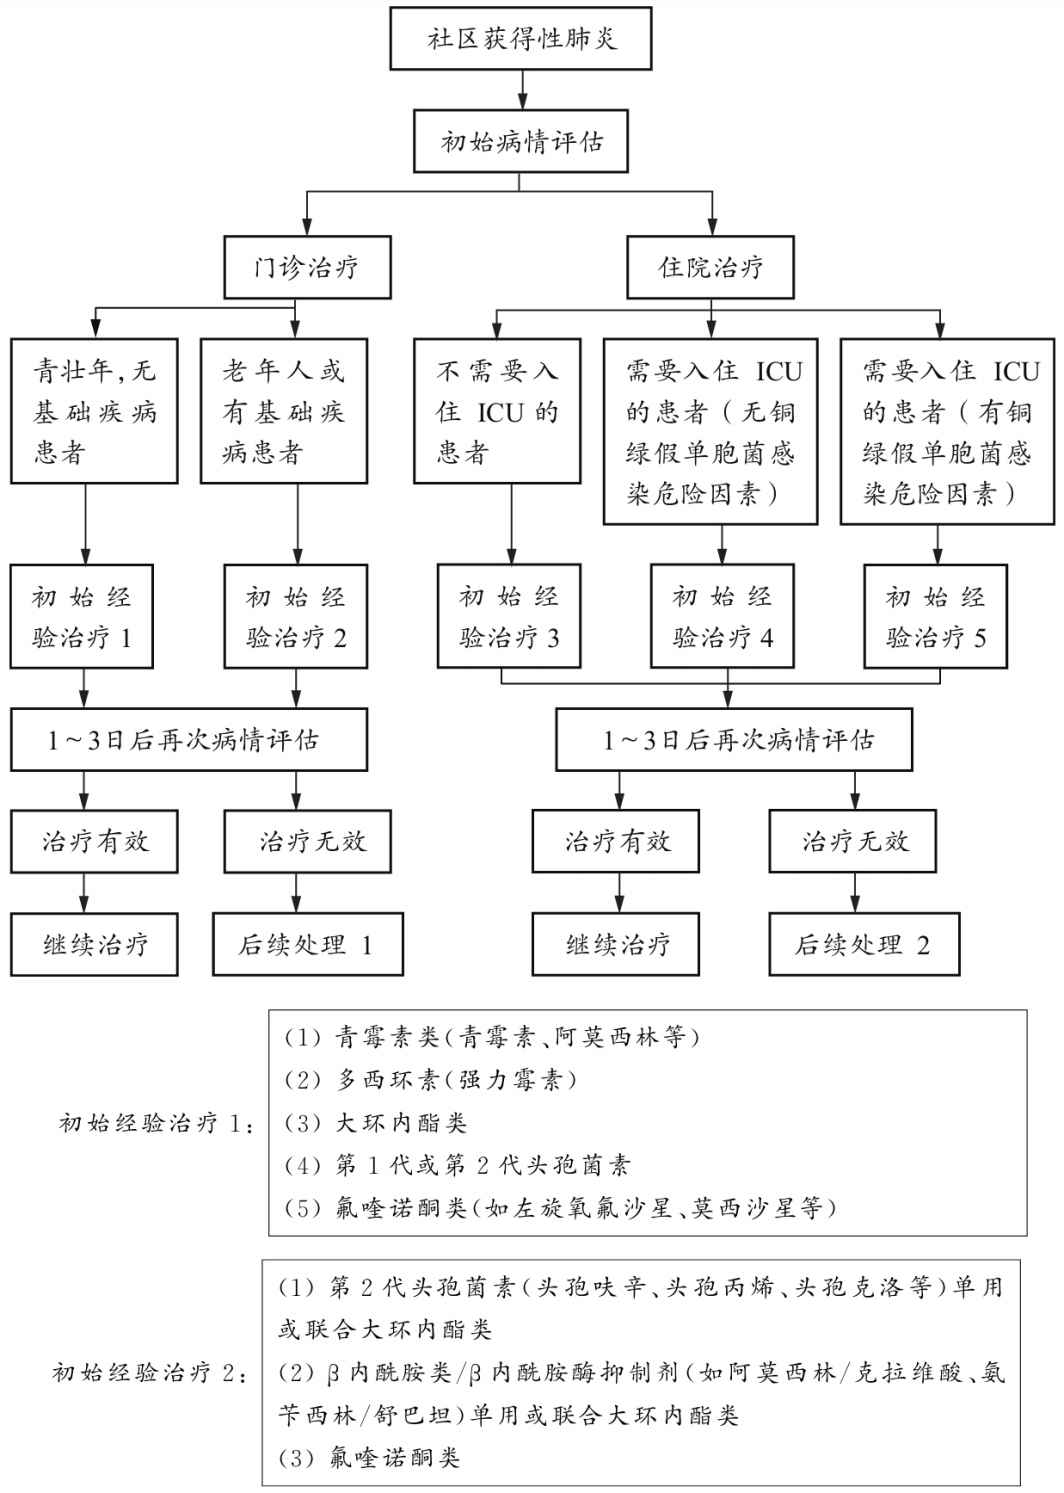
\includegraphics{./images/Image00015.jpg}
    \end{minipage}
\begin{minipage}[b]{0.49\textwidth} 
  \centering
  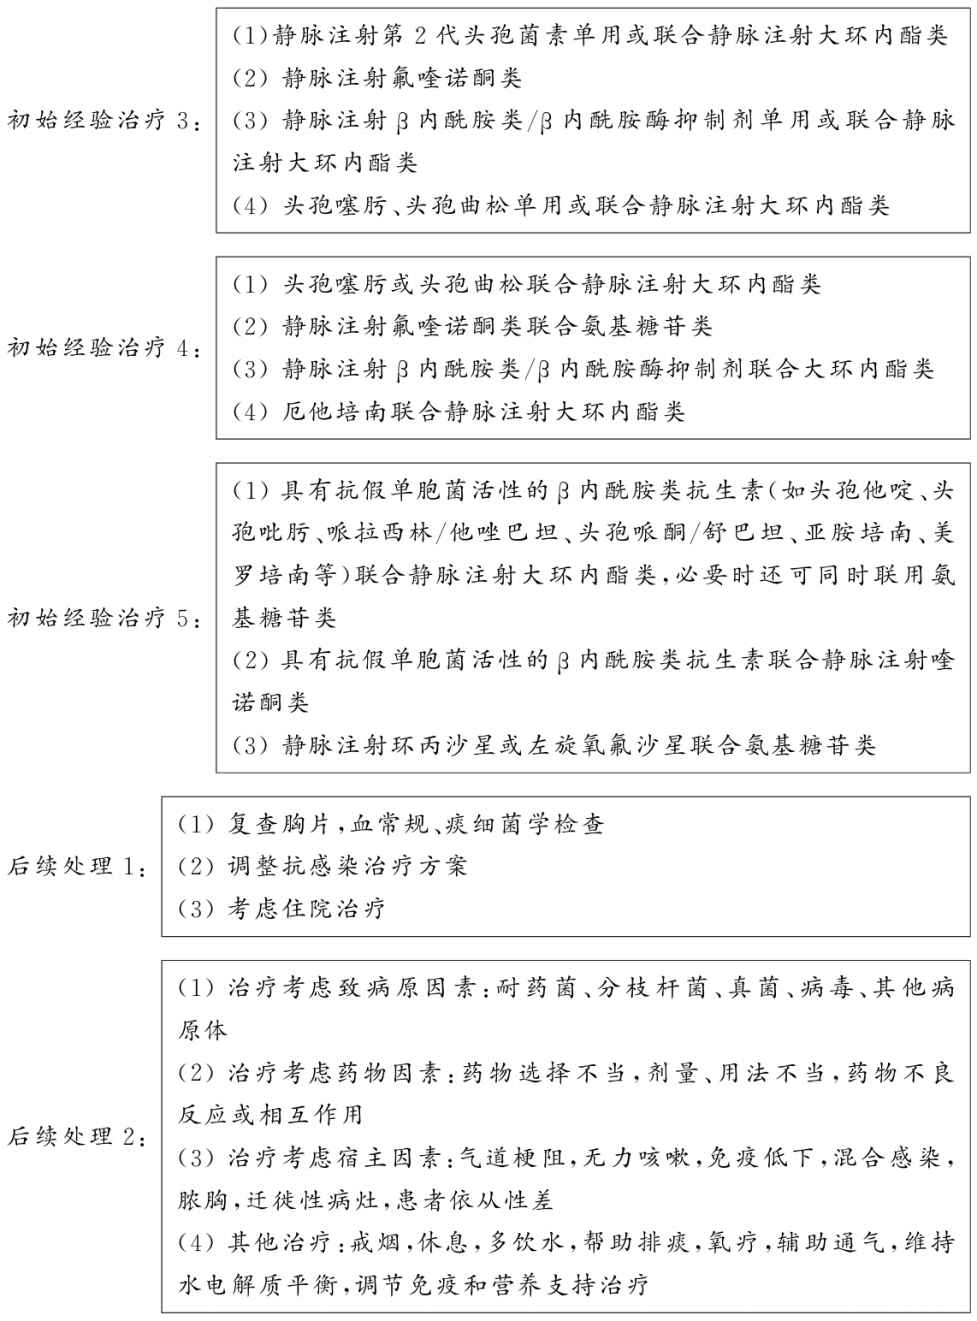
\includegraphics{./images/Image00016.jpg}
\end{minipage}
\captionsetup{justification=centering}
\caption{社区获得性肺炎的治疗程序}
\label{fig1-8-1a}
\end{figure} 

【治疗方案】

{(一)一般治疗}  戒烟,休息,多饮水,注意分泌物引流,氧疗。

{(二)药物及相关治疗}

1.
经验性抗菌治疗 CAP患者开始治疗初期,往往还没有病原学诊断的结果,此时应首先进行经验性抗菌治疗,具体参见本节的“治疗程序”。

2.
针对病原菌的治疗 CAP经临床和实验室有关检查,已经明确或高度怀疑某种病原菌,此时抗菌治疗就可以有的放矢,根据已确定的病原菌选择抗菌药物治疗的方案见表\ref{tab1-8-1}。


\begin{longtable}[]{p{3.5cm}p{6cm}p{6cm}}
  \caption{根据病原菌选用抗菌药物治疗}
  \label{tab1-8-1}\\
\toprule
病原菌 & 首先抗菌药物 & 其他抗菌药物的选择\tabularnewline
\midrule
\endfirsthead
\caption[]{根据病原菌选用抗菌药物治疗}\\
\toprule
病原菌 & 首先抗菌药物 & 其他抗菌药物的选择\tabularnewline
\midrule
\endhead
\midrule
\endfoot
\rowcolor{lightgray}肺炎链球菌 & &\tabularnewline
\rowcolor{lightgray} 青霉素敏感 & 青霉素G或青霉素V,阿莫西林 &
头孢菌素、大环内酯类、克拉霉素、氟喹诺酮类、多西环素\tabularnewline
\rowcolor{lightgray} 青霉素中度耐药 & 静脉用青霉素、头孢曲松或头孢噻肟钠、氟喹诺酮类 &
克拉霉素、多西环素、口服头孢菌素\tabularnewline
\rowcolor{lightgray} 青霉素高度耐药 & 氟喹诺酮类、万古霉素、利奈唑胺等均需按照药敏结果选择
& 克拉霉素、多西环素、头孢菌素、大环内酯类\tabularnewline
流感嗜血杆菌 &
第2、3代头孢菌素、多西环素、β内酰胺类/β内酰胺酶抑制剂、氟喹诺酮类 &
阿奇霉素、复方新诺明\tabularnewline
\rowcolor{lightgray}卡他莫拉菌 & 第2、3代头孢菌素、复方新诺明、阿莫西林/克拉维酸 &
大环内酯类、氟喹诺酮类\tabularnewline
厌氧菌 & 克拉霉素、青霉素+甲硝唑、β内酰胺类/β内酰胺酶抑制剂 &
青霉素G或青霉素V、氨苄西林/阿莫西林单用或合用甲硝唑\tabularnewline
\rowcolor{lightgray}金黄色葡萄球菌 & &\tabularnewline
\rowcolor{lightgray} \vtop{\hbox{\strut  甲氧西林敏感}\hbox{\strut (MSSA)}}&
新青霉素Ⅲ/苯唑西林,单用或合用利福平或庆大霉素 &
头孢唑林或头孢呋辛、万古霉素、克拉霉素、复方新诺明\tabularnewline
\rowcolor{lightgray} \vtop{\hbox{\strut  甲氧西林耐药}\hbox{\strut (MRSA)}}&
万古霉素单用或合用利福平或庆大霉素 & 利奈唑胺\tabularnewline
肠杆菌科(大肠杆菌、克雷伯菌、变形杆菌、肠杆菌) &
第3代头孢菌素单用或合用氨基糖苷类、碳青霉烯类 &
氨曲南、β内酰胺类/β内酰胺酶抑制剂、氟喹诺酮类\tabularnewline
\rowcolor{lightgray}铜绿假单胞菌 & 氨基糖苷类+抗假单胞菌β内酰胺类、碳青霉烯类 &
氨基糖苷类+环丙沙星、环丙沙星+抗假单胞菌β内酰胺类\tabularnewline
非典型病原体 & &\tabularnewline
 军团菌 & 大环内酯类单用或合用利福平、氟喹诺酮类 &
多西环素单用或合用利福平\tabularnewline
 支原体 & 多西环素、大环内酯类、氟喹诺酮类 &\tabularnewline
 衣原体 & 多西环素、大环内酯类、氟喹诺酮类 &\tabularnewline
 鹦鹉热衣原体 & 多西环素 & 红霉素、氯霉素\tabularnewline
\rowcolor{lightgray}诺卡菌 & 磺胺嘧啶单用或合用米诺环素或阿米卡星、复方新诺明 &
泰能单用或合用阿米卡星、多西环素或米诺环素\tabularnewline
伯纳特立克次体 & 四环素 & 氯霉素\tabularnewline
\end{longtable}

3. 对症及支持治疗

(1)解热镇痛:诊断明确后,对高热患者可给予解热镇痛药,如对乙酰氨基酚、阿司匹林、布洛芬等药。

(2)止咳祛痰:对痰液粘稠者,推荐使用祛痰药。如愈创甘油醚,每次10\textasciitilde{}20ml口服,每日3次;氨溴索,每次30mg口服,每日3次;溴己新,每次8\textasciitilde{}16mg口服,每日3次;标准桃金娘油胶囊,每次0.3\textasciitilde{}0.6g口服,每日3次。通常避免使用止咳药物,对于剧烈咳嗽,无痰或少痰,而严重影响休息者,可临时采用。如右美沙芬,每次15\textasciitilde{}30mg口服,每日3\textasciitilde{}4次;苯丙哌林,每次20\textasciitilde{}40mg口服,每日3次。

(3)支持治疗:注意维持水电解质平衡,调节免疫,纠正低蛋白血症和营养支持治疗。

4.
其他治疗 对于重症患者,伴低氧血症者必要时给予辅助通气,伴急性肾衰竭者给予透析治疗。

【疗效观察与随访】

1. 观察指标

(1)初始治疗后2\textasciitilde{}3日应对病情和诊断进行评价。有效治疗反应首先表现为体温下降,呼吸道症状亦可以有改善。白细胞恢复和X线胸片病灶吸收一般出现较迟。凡症状明显改善,不一定考虑痰病原学检查结果如何,仍可维持原有治疗。症状显著改善后,胃肠外给药者可改用同类或抗菌谱相近、或对致病原敏感的制剂口服给药,采用序贯治疗。

(2)初始治疗3日后症状无改善或一度改善又恶化,视为治疗无效,其常见原因和处理如下:①药物未能覆盖致病菌或细菌耐药,结合实验室痰培养结果并评价其意义,审慎调整抗感染药物,并重复病原学检查。②特殊病原体感染,如分枝杆菌、真菌、肺孢子菌、包括SARS和人禽流感在内的病毒或地方性感染性疾病。应重新对有关资料进行分析并进行相应检查,包括对通常细菌的进一步检测,必要时采用侵袭性检查技术,明确病原学诊断并调整治疗方案。③出现并发症(脓胸、迁徙性病灶等)或存在影响疗效的宿主因素(如免疫损害),应进一步检查和确认,进行相应处理。④CAP诊断有误时,应重新核实CAP的诊断,明确是否为非感染性疾病。

2.
疗效评估 治愈标准:症状、体征消失,血象正常,胸部X线检查示病灶完全消失,无并发症。

3.
随访 根据治疗后72小时的反应进行抗菌治疗的再评估,如果疗效好,即可维持治疗或序贯治疗,如果疗效差,注意根据相关检查结果调整治疗方案。

【治疗经验与解析】

1.
应根据特定病原体的危险因素决定治疗用药 如果患者合并某些危险因素(表\ref{tab1-8-2})或存在某些合并症(表\ref{tab1-8-3}),将有感染某种特定病原体的可能,治疗时应予考虑。


\begin{longtable}[]{lp{7cm}}
  \caption{增加特定细菌感染风险的危险因素}
  \label{tab1-8-2}\\
\toprule
特定细菌 & 危险因素\tabularnewline
\midrule
\endhead
耐药肺炎链球菌 &
年龄\textless{}65岁;近3个月内应用过β内酰胺类抗生素治疗;酗酒;多种临床合并症;免疫抑制性疾病(包括应用糖皮质激素治疗);接触日托中心儿童\tabularnewline
军团菌属 &
吸烟;细胞免疫缺陷,如器官移植;肾衰竭或肝功能衰竭;糖尿病;恶性肿瘤\tabularnewline
肠道革兰阴性杆菌 &
居住在养老院;心、肺基础病;多种临床合并症;近期应用过抗生素治疗\tabularnewline
铜绿假单胞菌 &
结构性肺疾病(支气管扩张症、肺囊性纤维化、弥漫性泛细支气管炎等);应用糖皮质激素(泼尼松\textgreater{}10mg/日);过去1个月中广谱抗生素应用\textgreater{}7日;营养不良;外周血中性粒细胞计数\textless{}1×10$^{9}$
/L\tabularnewline
\bottomrule
\end{longtable}

\begin{longtable}[]{lp{7cm}}
  \caption{某些特定状态下CAP患者易感染的病原体}
  \label{tab1-8-3}\\
\toprule
状态或合并症 & 易感染的特定病原体\tabularnewline
\midrule
\endhead
酗酒 &
肺炎链球菌(包括耐药的肺炎链球菌)、厌氧菌、肠道革兰阴性杆菌、军团菌属\tabularnewline
COPD/吸烟者 & 肺炎链球菌、流感嗜血杆菌、卡他莫拉菌\tabularnewline
居住在养老院 &
肺炎链球菌、肠道革兰阴性杆菌、流感嗜血杆菌、金黄色葡萄球菌、厌氧菌、肺炎衣原体\tabularnewline
患流感 & 金黄色葡萄球菌、肺炎链球菌、流感嗜血杆菌\tabularnewline
接触鸟类 & 鹦鹉热衣原体、新型隐球菌\tabularnewline
疑有吸入因素 & 厌氧菌\tabularnewline
结构性肺病 &
铜绿假单胞菌、洋葱伯克霍尔德菌、金黄色葡萄球菌\tabularnewline
近期应用抗生素 &
耐药肺炎链球菌、肠道革兰阴性杆菌、铜绿假单胞菌\tabularnewline
\bottomrule
\end{longtable}

2.
CAP经验性抗菌治疗的注意事项 CAP患者治疗初期经验性抗菌治疗选择抗菌药物要考虑许多因素,包括疾病的严重程度、患者的年龄、对抗菌药物的耐受性或副作用、临床表现、联合用药情况、接触史和流行病学史等。还需要考虑选择药物的剂量、药效药动学特征,抗菌治疗疗程等。

(1)对于既往健康的轻症且胃肠道功能正常的患者:应尽量推荐用生物利用度良好的口服抗感染药物治疗。

(2)我国成人CAP致病肺炎链球菌:对青霉素的不敏感率(包括中介与耐药)在20\%左右,青霉素中介水平耐药肺炎链球菌肺炎仍可选择青霉素,但需提高剂量,如青霉素G240万U静脉滴注,每4\textasciitilde{}6小时1次。高水平耐药或存在耐药高危险因素时应选择头孢曲松、头孢噻肟、厄他培南、氟喹诺酮类或万古霉素。

(3)我国肺炎链球菌:对大环内酯类耐药率普遍在60\%以上,且多呈高水平耐药,因此,在怀疑为肺炎链球菌所致CAP时不宜单独应用大环内酯类,但大环内酯类对非典型致病原仍有良好疗效。

(4)支气管扩张症并发肺炎:铜绿假单胞菌是常见病原体,经验性治疗药物选择应兼顾及此。除上述推荐药物外,亦有人提倡联合喹诺酮类或大环内酯类,据认为此类药物易穿透或破坏细菌的生物被膜。

(5)疑有吸入因素时:应优先选择氨苄西林/舒巴坦、阿莫西林/克拉维酸等有抗厌氧菌作用的药物,或联合应用甲硝唑、克林霉素等,也可选用莫西沙星等对厌氧菌有效的氟喹诺酮类药物。

(6)对怀疑感染流感病毒的患者:一般并不推荐联合应用经验性抗病毒治疗,只有对于有典型流感症状(发热、肌痛、全身不适和呼吸道症状)、发病时间\textless{}2日的高危患者及处于流感流行期时,才考虑联合应用抗病毒治疗。

(7)对于危及生命的重症肺炎:建议早期采用广谱强效的抗菌药物治疗,待病情稳定后可根据病原学进行针对性治疗,或降阶梯治疗。抗生素治疗要尽早开始,首剂抗生素治疗争取在诊断CAP后4小时内使用,以提高疗效,降低病死率,缩短住院时间。

(8)抗感染治疗:一般可于热退和主要呼吸道症状明显改善后3\textasciitilde{}5日停药,但疗程视不同病原体、病情严重程度而异,不宜将肺部阴影完全吸收作为停用抗菌药物的指征。对于普通细菌性感染,如肺炎链球菌,用药至患者热退后3日即可;对于金黄色葡萄球菌、铜绿假单胞菌、克雷伯菌属或厌氧菌等容易导致肺组织坏死的致病菌所致的感染,建议抗菌药物疗程≥2周。对于非典型病原体,疗程应略长,如肺炎支原体、肺炎衣原体感染的建议疗程为10\textasciitilde{}14日,军团菌属感染的疗程建议为10\textasciitilde{}21日。

(9)重症肺炎:除有效抗感染治疗外,营养支持治疗和呼吸道分泌物引流亦十分重要。

\subsection{医院获得性肺炎}

医院获得性肺炎(hospital-acquired
pneumonia,HAP)亦称医院内肺炎(nosocomial
pneumonia,NP),是指患者入院时不存在、也不处于感染潜伏期,而于入院48小时后在医院(包括老年护理院、康复院)内发生的肺炎。包括呼吸机相关性肺炎(VAP)和健康护理相关肺炎(HCAP)。国际上多数报道HAP发病率0.5\%\textasciitilde{}1.0\%,在西方国家居医院感染的第2\textasciitilde{}4位;ICU内发病率15\%\textasciitilde{}20\%,其中接受机械通气患者高达18\%\textasciitilde{}60\%,病死率超过50\%。我国HAP发病率1.3\%\textasciitilde{}3.4\%,是第1位的医院内感染(占29.5\%)。HAP在病原学、流行病学和临床诊治上与CAP有显著不同。

【治疗程序】 图\ref{fig1-8-2}所示。

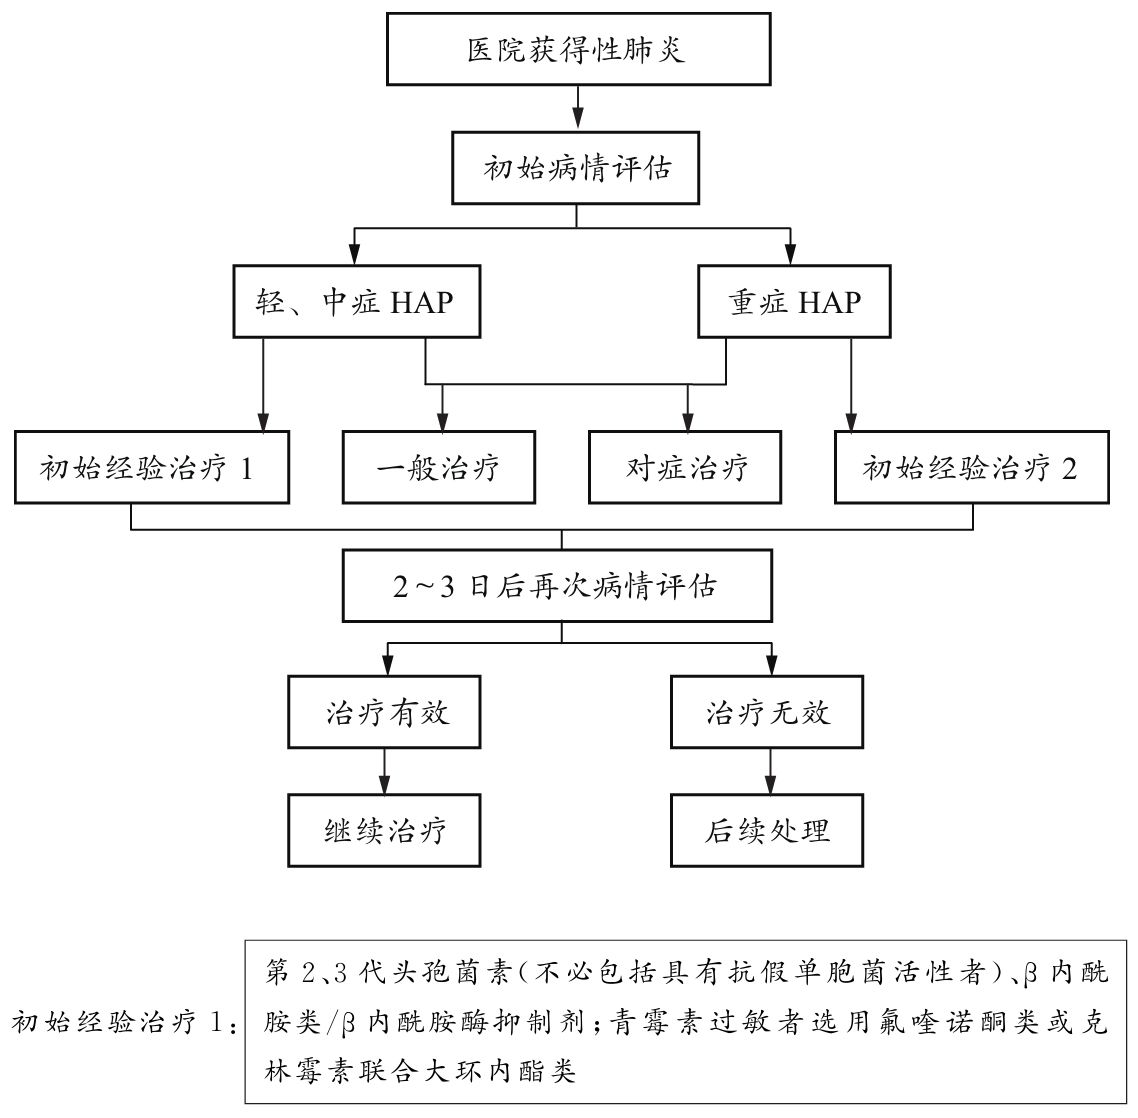
\includegraphics{./images/Image00017.jpg}
\begin{figure}[!htbp]
 \centering
 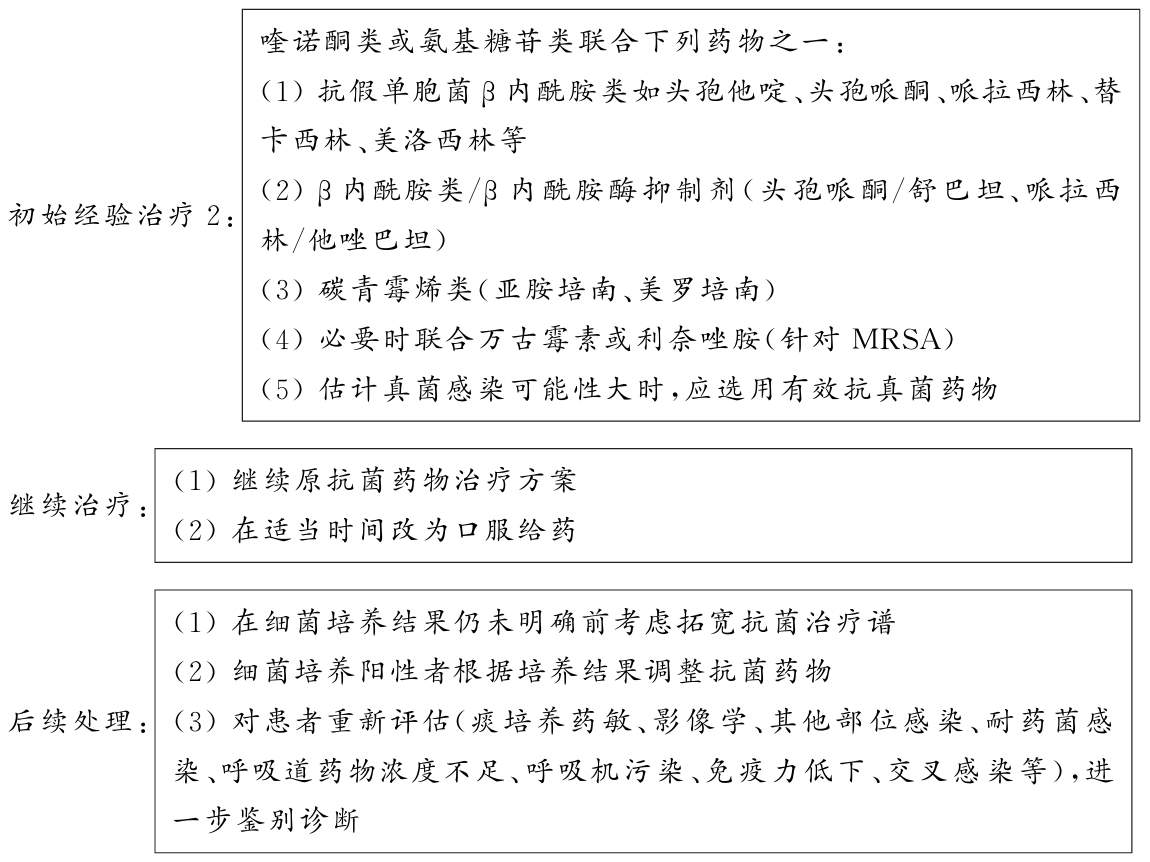
\includegraphics{./images/Image00018.jpg}
 \captionsetup{justification=centering}
 \caption{医院获得性肺炎的治疗程序}
 \label{fig1-8-2}
  \end{figure} 

【治疗方案】

{(一)一般治疗}  戒烟,休息,多饮水,注意分泌物引流,氧疗。

{(二)药物及相关治疗}

1.
经验性抗菌治疗 HAP患者开始治疗初期,往往还没有病原学诊断的结果,此时应首先进行经验性抗菌治疗,具体参见本节的“治疗程序”。

2.
针对病原菌的治疗 HAP经临床和实验室有关检查,已经明确或高度怀疑某种病原菌,此时抗菌治疗就可以有的放矢,根据已确定的病原菌选择抗菌药物治疗的方案见表\ref{tab1-8-4}。

\begin{longtable}[]{p{3.5cm}p{6cm}p{6cm}}
  \caption{根据病原菌选用抗菌药物治疗}
  \label{tab1-8-4}\\
\toprule
病原菌 & 首先抗菌药物 & 其他抗菌药物的选择\tabularnewline
\midrule
\endhead
\rowcolor{lightgray}金黄色葡萄球菌 & &\tabularnewline
\rowcolor{lightgray}\vtop{\hbox{\strut  甲氧西林敏感}\hbox{\strut (MSSA)}} &
新青霉素Ⅲ/苯唑西林,单用或合用利福平或庆大霉素 &
头孢唑啉或头孢呋辛、克林霉素、氟喹诺酮类、复方新诺明\tabularnewline
\rowcolor{lightgray}\vtop{\hbox{\strut  甲氧西林耐药}\hbox{\strut (MRSA)}} &
(去甲)万古霉素单用或联合利福平或奈替米星 &
氟喹诺酮类、碳青霉烯类或替考拉宁、利奈唑胺(须经体外药敏试验)\tabularnewline
肠杆菌科(大肠杆菌、克雷伯菌、变形杆菌、肠杆菌属等) &
第2、3代头孢菌素联合氨基糖苷类(参考药敏试验可以单用) &
氟喹诺酮类、氨曲南、亚胺培南、美罗培南、β内酰胺类/β内酰胺酶抑制剂\tabularnewline
\rowcolor{lightgray}流感嗜血杆菌 & 第2、3代头孢菌素、新大环内酯类、复方新诺明、氟喹诺酮类 &
β内酰胺类/β内酰胺酶抑制剂(氨苄西林/舒巴坦钠、阿莫西林/克拉维酸)\tabularnewline
铜绿假单胞菌 &
氨基糖苷类、抗假单胞菌β内酰胺类(如哌拉西林/他唑巴坦、替卡西林/克拉维酸、美洛西林、头孢他啶、头孢哌酮/舒巴坦等)及氟喹诺酮类
& 氨基糖苷类联合氨曲南、亚胺培南、美罗培南\tabularnewline\rowcolor{lightgray}
不动杆菌 & 亚胺培南或氟喹诺酮类联合阿米卡星或头孢他啶、头孢哌酮/舒巴坦
&\tabularnewline
军团杆菌 & 红霉素或联合利福平、环丙沙星、左氧氟沙星 &
新大环内酯类联合利福平、多西环素联合利福平、氧氟沙星\tabularnewline\rowcolor{lightgray}
厌氧菌 & 青霉素联合甲硝唑、克林霉素、β内酰胺类/β内酰胺酶抑制剂 &
替硝唑、氨苄西林、阿莫西林、头孢西丁\tabularnewline
真菌 &
氟康唑,酵母菌(新型隐球菌)、酵母样菌(念珠菌属)和组织胞浆菌大多对氟康唑敏感。两性霉素B抗菌谱最广,活性最强,但不良反应重,当感染严重或上述药物无效时可选用
&
氟胞嘧啶(念珠菌、隐球菌);咪康唑(芽生菌属、组织胞浆菌属、隐球菌属、部分念珠菌);伊曲康唑(曲菌、念珠菌、隐球菌等)\tabularnewline\rowcolor{lightgray}
巨细胞病毒 &
更昔洛韦单用或联合静脉用免疫球蛋白(IVIG)、或巨细胞病毒高免疫球蛋白 &
膦甲酸钠\tabularnewline
肺孢子菌 & 复方新诺明 & 喷他脒、氨苯砜合用甲氧苄啶\tabularnewline
\bottomrule
\end{longtable}

3.
其他治疗 注意解热镇痛、止咳祛痰、支持治疗,注意维持水电解质平衡,调节免疫,纠正低蛋白血症和营养支持治疗,具体内容同CAP。加强呼吸治疗,如吸氧和机械通气。

【疗效观察与随访】

1. 观察指标

(1)在进行抗生素治疗前,必须采集下呼吸道标本进行病原学培养(定量或半定量)和血培养。进行X线胸片检查和测动脉血氧饱和度,在初始治疗后2\textasciitilde{}3日应对病情和诊断进行评价,具体内容同CAP。

(2)初始治疗3日后症状无改善或一度改善又恶化,视为治疗无效,其常见原因和处理如下:

①HAP抗菌治疗无效常见原因:a.诊断不可靠:非感染性原因、病原学诊断不明或评估错误。b.病原体清除困难:耐药、呼吸道药物浓度不足(药物或解剖因素)、感染的肺外扩散、呼吸机有关污染源持续存在、宿主免疫防御机制损害。c.二重感染或肺外扩散。d.因药物不良反应,用药受限。e.系统性炎症反应被激发,肺损伤甚至多器官功能衰竭。

②处理:a.确立可靠病原学诊断,参考药敏或血药浓度等相关测定,慎重和周密地制定或调整治疗方案。b.消除污染源,防止交叉感染。c.防止其他可能引发或加重肺损伤的因素。

2. 疗效评估 治愈标准:参见CAP。

3.
随访 根据治疗后3日的反应进行抗菌治疗的再评估,如果疗效好,即可维持治疗或序贯治疗,如果疗效差,注意根据相关检查结果调整治疗方案。

【治疗经验与解析】

1. 应根据危险因素与病原学分布的特点,选择合适的抗感染治疗(表\ref{tab1-8-5})。

\begin{longtable}[]{lp{8cm}}
  \caption{增加特定细菌感染风险的危险因素}
  \label{tab1-8-5}\\
\toprule
特定细菌 & 危险因素\tabularnewline
\midrule
\endhead
铜绿假单胞菌、不动杆菌属和肠道菌属 &
长期重症监护患者;应用糖皮质激素;发病前接受抗生素治疗;结构性肺疾病(支气管扩张症、肺囊性纤维化、弥漫性泛细支气管炎等)\tabularnewline
金黄色葡萄球菌 &\tabularnewline
 MSSA &
昏迷;头部创伤;糖尿病;肾衰;静脉注射毒品;近期患流感\tabularnewline
 MRSA & 病原菌流行区;发病前接受抗生素治疗;长期住院\tabularnewline
厌氧菌 & 近期胸腹手术;吸入史;异物阻塞气道\tabularnewline
军团菌属 & 病原菌流行区;使用大剂量糖皮质激素、免疫抑制剂\tabularnewline
\bottomrule
\end{longtable}

2.
HAP抗菌治疗的药物选择要点 ①抗菌药物对引起HAP呼吸道病原体的敏感性。②抗生素的过敏病史:由于β内酰胺类抗生素有交叉过敏的可能性,对有青霉素过敏的患者应用头孢菌素应十分谨慎。③抗菌治疗时应该选用药物间相互作用最小的药物。④对肝肾功能不全的患者,需选用特殊药物以避免调整剂量。⑤注意抗菌药物的潜在副作用,在某些特殊患者中应考虑到其相对禁忌证(如对患有神经肌肉疾患或有肾功能不全的患者应避免使用氨基糖苷类抗生素)。⑥患者因素:年龄、妊娠和哺乳等限制某些抗生素的应用。⑦如果疗效和副作用相似,选用价格低廉的药物。⑧药物的抗菌作用机制与选用的抗生素和剂量相关。通常优先选用杀菌的抗生素而不选用抑菌的抗生素。β内酰胺类抗生素和万古霉素均为杀菌药物,并且与时间相关。氨基糖苷类和喹诺酮类抗菌药物也为杀菌药物,但属于浓度依赖性药物,在高浓度时能迅速杀灭病原体。

3.
HAP初始经验性抗菌治疗无效的原因 ①诊断错误,有很多其他原因临床上被误认为HAP,如肺栓塞、肺不张、肺泡出血、ARDS、肺肿瘤。②宿主原因,如高龄、机械通气时间长、呼吸衰竭、潜在致死性疾病、双侧肺浸润、抗生素治疗史等。③细菌因素,初始治疗未覆盖某些耐药菌,如铜绿假单胞菌、不动杆菌属。或者其他少见病原体(结核分枝杆菌、真菌、呼吸道病毒等)。另外,在治疗过程中,可能出现导致发热的并发症,如鼻窦炎、静脉导管相关感染、假膜性肠炎、泌尿系感染等。

4.
HAP应尽早给予抗生素治疗 严重HAP患者必须使用充足剂量的抗生素以保证最大的疗效。ATS推荐,肾功能正常的成年患者,常用头孢吡肟和头孢他啶的充分治疗剂量是2g,q8h;而美罗培南的治疗剂量(1g,q8h)通常要略大于亚胺培南(0.5g,q8h);哌拉西林/他唑巴坦的剂量不仅每次用药至少要4.5g,而且每日用药次数为4次;在氨基糖苷类药物中,阿米卡星的每日剂量为20mg/kg;而喹诺酮类中环丙沙星为400mg,q8h,左氧氟沙星为750mg,qd。应引起我国临床医生的重视,提示在临床实践中可能存在治疗剂量不足的情况。

循证医学证据表明,对HAP的治疗如果有效,通常在前6日就有临床表现明显改善。此时延长治疗14日或更长时间,反而容易导致新的细菌寄殖,尤其是铜绿假单胞菌和肠杆菌科细菌。如果患者接受了适当的初始抗生素方案,只要病原菌不是铜绿假单胞菌,患者有良好的临床反应,感染的临床表现缓解,应努力将抗生素的疗程从传统的14\textasciitilde{}21日缩短为7\textasciitilde{}8日。如果患者采用的联合治疗方案中包括了氨基糖苷类,只要患者有反应,可以在5日后停用氨基糖苷类。

5.
特殊病原体感染的抗生素治疗方案 临床最常见的4种MDR病原菌为铜绿假单胞菌、不动杆菌、产ESBLs肠杆菌科细菌和MRSA。对铜绿假单胞菌推荐联合治疗,主要是使用β内酰胺类联合氨基糖苷类,可替代后者的是氟喹诺酮类,主要为环丙沙星或左氧氟沙星。治疗不动杆菌属最有效的药物是碳青霉烯类、舒巴坦、多粘菌素E和多粘菌素B,近来报道替加环素也有良好的疗效。而当分离到产ESBLs肠杆菌科细菌时应避免使用第3代头孢菌素单药治疗,尤其肠杆菌属细菌,最有效的药物是碳青霉烯类。对于MRSA已有大规模多中心试验证实利奈唑胺与万古霉素的疗效相当,因此肾功能不全的患者,或正在接受其他肾毒性药物,可以优先考虑利奈唑胺。

6.
有效的感染控制措施是对医护人员教育 遵循用含乙醇消毒液洗手,隔离MDR感染者,防止交叉感染。监测ICU感染,鉴定和定量地区性的和新出现的MDR病原菌,准备适时的感染控制资料,对可疑VAP或其他医院感染患者指导适宜的抗微生物治疗。

7.
气管插管和机械通气要点 ①插管和再插管应尽可能避免,因可导致VAP的危险。②无创通气对急性呼吸衰竭的患者应尽可能选择应用。③尽管直接的因果关系尚未证实,在预防医院获得性鼻窦炎和减少VAP危险上,经口插管和经口胃管优于经鼻的途径。④持续声门下吸引可减少早发性VAP危险,应尽可能使用。⑤气管插管气囊压力应保持在20cmH{2}
O以上,以避免气囊周围细菌渗漏入下呼吸道。⑥呼吸机管道内污染的冷凝水应避免进入气管插管内或沾在管道上和雾化器内。⑦被动湿化器或加热湿化交换器减少呼吸管道内细菌定植,但不减少VAP的发生率。⑧缩短插管和机械通气时间能预防VAP。⑨保持ICU医护人员合适的水平能减少住院时间,改善感染控制,减少机械通气时间。

8.
患者应保持半坐卧位(30°\textasciitilde{}45°)以预防误吸,尤其是在喂食时。应优先选用肠内营养,以减少中心静脉管的并发症,预防肠粘膜绒毛萎缩和增加细菌易位危险。

9.
调节定植要点 ①常规口服抗生素(SDD)可减少ICU中VAP的发生率,帮助控制MDR细菌暴发,但不推荐常规使用。②在某些患者群体先前的全身抗生素使用能减少HAP的危险,但如果有在感染已经发生时使用抗生素病史,则有增加MDR病原体感染的可能性。

\subsection{免疫损害宿主肺炎}

免疫损害宿主(immunocompromised
host,ICH)是按其起因分为先天性和获得性,按其防御机制分为特异性和非特异性。前者又区分为B细胞介导免疫和T细胞介导免疫损害,后者主要有中性粒细胞数量减少或功能异常、补体缺乏和物理屏障损害(如体内留置导管、气管插管/切开等)。而临床上通常按其病因粗略区分为HIV/AIDS和非HIV/AIDS。ICH不断增加和累积,成为一个全球性的巨大挑战。感染是影响ICH病程和预后的最重要因素,肺是感染的主要靶器官。免疫损害宿主肺炎已不仅是医院感染的主要疾病,而且在社区感染中也在增加和引起关注。本节主要讨论非HIV/AIDS的肺炎。

【治疗程序】 图\ref{fig1-8-3}所示。

\begin{figure}[!htbp]
 \centering
 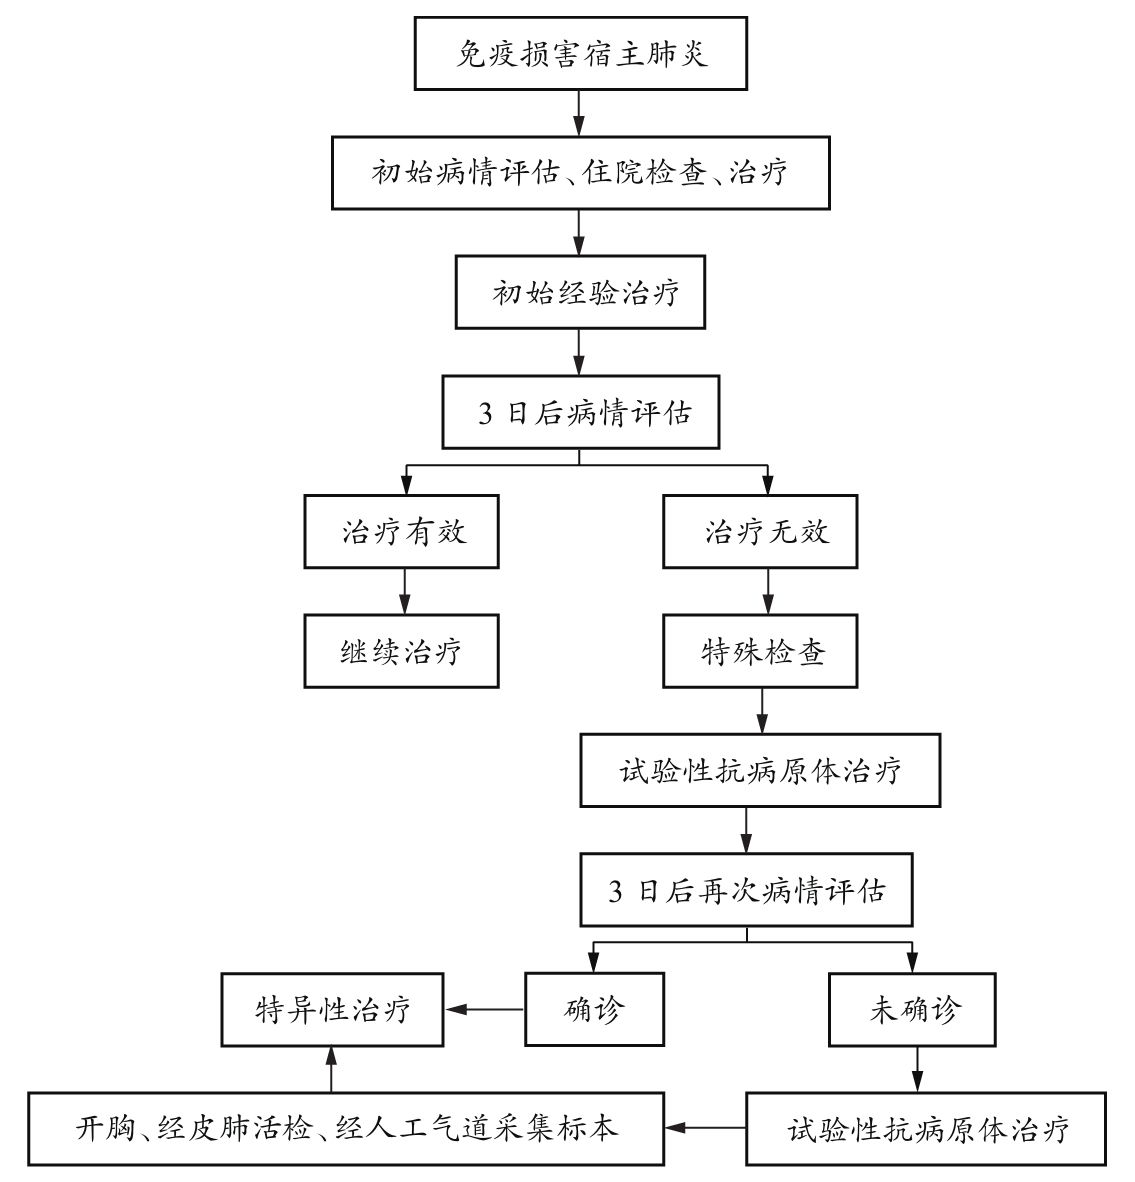
\includegraphics{./images/Image00019.jpg}
 \captionsetup{justification=centering}
 \caption{免疫损害宿主肺炎的治疗程序}
 \label{fig1-8-3}
  \end{figure} 

【治疗方案】

{(一)一般治疗}
 注意免疫重建治疗和支持治疗。尽可能停用或减量使用免疫抑制药物,集落刺激因子(G-CSF或GM-CSF)可增加白细胞数和吞噬功能,可应用于白细胞减少患者,先天性IgG减少和重症患者补充IgG具有肯定价值。营养、心肺功能和心理支持都十分重要,有指征者应气管插管机械通气治疗。

{(二)药物治疗}

1.
细菌感染 根据病原体培养和药敏结果,可选用第3、4代头孢菌素,碳青霉烯类抗生素,β内酰胺类/β内酰胺酶抑制剂,糖肽类抗生素,新一代氟喹诺酮,或以上药物与氨基糖苷联合用药。具体可参见CAP、HAP章节。

2.
病毒感染 应采取对症处理及使用金刚烷胺、阿昔洛韦(无环鸟苷)、阿糖胞苷、利巴韦林(病毒唑)等,而丙氧鸟苷对巨细胞病毒(CMV)感染有一定疗效。干扰素可干扰病毒复制及合成和促进吞噬作用,对病毒感染早期有一定疗效。此外,特异性Ig被动免疫、病毒疫苗以及中草药大青叶、板蓝根等亦可使用。

3.
真菌感染 针对真菌的种类及药敏试验结果,可选用氟康唑、伊曲康唑、氟胞嘧啶、两性霉素B、伏立康唑、卡泊芬净等。如肺孢子菌(PC)可选用SMZ+TMP、喷他脒(戊烷脒)或氨苯砜+TMP。

4. 原虫感染 如弓形体应用乙胺嘧啶+磺胺嘧啶治疗。

5.
不典型病原体感染 支原体感染可选用大环内酯类或氟喹诺酮类抗菌药物,如为衣原体感染则应用四环素类或大环内酯类抗生素治疗。

HAP患者开始治疗初期,往往还没有病原学诊断的结果,此时应首先进行经验性抗菌治疗,具体参见本节的“治疗程序”。

【疗效观察与随访】

1. 观察指标

(1)肺部病变的早期发现和病因鉴别:早期发现和确诊直接影响预后,如肾移植受者的发热和肺浸润在5日内发现和确诊者存活率为79\%,而延误超过5日者仅35\%。应加强临床观察,不放过任何细微的症状和体征。PaO{2}
对移植受者肺部疾病的早期发现和诊断有一定的帮助,约80\%的细菌性肺炎和70\%肺栓塞患者PaO{2}
\textless{}65mmHg,而病毒、PCP、真菌或诺卡菌肺炎仅有8\%的患者PaO{2}
低于此限。X线检查对诊断虽非特异性,但仍是有帮助的。局限性病变常见于细菌、真菌、军团菌、分枝杆菌、肺出血、肺栓塞,有时也见于早期PCP;结节或空洞性病变常为隐球菌、诺卡菌、曲霉、肺脓肿(包括迁徙性)、分枝杆菌和肿瘤;弥漫性间质性/腺泡浸润性病变多由于肺孢子菌肺炎(PCP)、病毒、弓浆虫、分枝杆菌、肺水肿(包括ARDS)、放射线/药物、癌性淋巴管炎等引起。核素肺扫描对PCP筛选和诊断有一定意义。CT对隐蔽部位如心脏移植后肺底部病变的发现和诊断很有价值。ICH发热伴肺浸润的病因颇多,准确的病因(原)诊断常常需要病原学或组织学证据。

(2)病原学诊断

①标本采集:除尽量收集各种可能有意义的肺外标本如体液、分泌物以及肿大淋巴结、体表肿物活检标本外,呼吸道标本仍是最基本和最重要的。痰液需经筛选、洗涤或定量培养等处理,以减少污染或减少结果解释上的困难。为避免污染以及在无痰患者则需从下呼吸道直接采样。

②微生物学检查:应当强调:a.标本必须新鲜,应及时送检和处理。b.检测项目尽可能齐全,涂片和培养(除培养不能生长的病原体)都应进行。因为PSB和活检标本少,仅供细菌和条件性真菌的培养,抗酸杆菌和原虫等检测只需吸引物或咳出物。故标本应该合理分配检查项目。此外对严重免疫抑制如器官移植、粒细胞缺乏患者应常规进行口咽部、肛周及会阴部皮肤等处的微生物学监测。

③免疫学诊断和基因诊断技术:抗体检测可能因宿主免疫抑制影响其价值。抗原和基因检测在理论上可提供早期诊断和很高的特异性和敏感性,但迄今前者仅限于极少数特殊病原体。

④组织学检查:组织学上坏死性肺炎见于化脓菌、真菌及CMV等感染。前者多无病原特异性,但若见到“假单胞菌血管炎”则对铜绿假单胞菌感染有诊断意义。通常细菌和真菌阴性,而炎症病灶中有较多巨噬细胞,则应考虑军团菌肺炎可能。借助银染色或PAS染色对真菌诊断有决定性意义。CMV肺炎在常规组织学上不易发现包涵体,需要应用组织化学及原位杂交方法揭示其抗原或DNA。并发于ICH的肺结核其组织学改变可以很不典型或呈现“无反应性结核”,应常规加做抗酸染色。PC在HE染色时可见脓染成黑色的菌体包囊壁,易于识别。在印片和涂片标本中检查PCP需要采用Giemsa或Wright-Giemsa特殊染色,可以发现染成红色或暗红色的囊内小体。

2. 疗效评估 疗效随病因不同而定,治愈标准,参见CAP。

3.
随访 根据治疗后3日的反应进行抗菌治疗的再评估,如果疗效好,即可维持治疗或序贯治疗,如果疗效差,注意根据相关检查结果调整治疗方案。

【治疗经验与解析】

1.
不同类型免疫损害在病原体分布上存在显著差异(表\ref{tab1-8-6}),应根据不同的病原体选用合适的治疗方案。

\begin{longtable}[]{p{3.6cm}p{5.7cm}p{5.7cm}}
  \caption{免疫损害类型与易感病原体}
  \label{tab1-8-6}\\
\toprule
免疫损害 & 常见情况 & 病原体\tabularnewline
\midrule
\endhead
\rowcolor{lightgray}粒细胞缺乏 & 肿瘤化疗、药物不良反应、白血病 & 细菌:需氧G{-}
杆菌(肠道菌群、假单胞菌)、金黄色葡萄球菌、草绿色链球菌真菌:曲霉\tabularnewline
细胞介导免疫损害 & 器官移植、HIV感染、淋巴瘤、皮质激素治疗 &
细菌:李斯特菌、沙门菌、诺卡菌、分枝杆菌、军团菌; 病毒:CMV、单纯疱疹病毒、水痘带状疱疹病毒; 寄生虫:弓形体、粪类圆线虫; 真菌:肺孢子菌、隐球菌、组织胞浆菌、球孢子菌\tabularnewline\rowcolor{lightgray}
低(无)丙种球蛋白血症 &
多发性骨髓瘤、先天性或获得性缺乏、慢性淋巴细胞性白血病 &
肺炎链球菌、流感嗜血杆菌\tabularnewline
补体缺乏 & 先天性 &
肺炎链球菌、流感嗜血杆菌、金黄色葡萄球菌、肠杆菌科细菌、脑膜炎奈瑟菌、肺炎链球菌\tabularnewline\rowcolor{lightgray}
中性粒细胞杀菌缺陷 & 慢性肉芽肿、髓过氧化物酶缺乏 &
金黄色葡萄球菌\tabularnewline
\bottomrule
\end{longtable}

2.
实体器官移植后感染具有不同特点,应注意选择合适的治疗 ①真菌感染多在术后2\textasciitilde{}3周,肝移植受者可以早在第一周。②术后早期(\textless{}1个月)细菌性肺炎多系强毒力致病菌,G{-}
杆菌、肺炎链球菌、金黄色葡萄球菌居前3位,合计占80\%以上。术后3\textasciitilde{}4周内的肺炎很少是机会致病菌。③CMV感染多见于术后1\textasciitilde{}4个月,而CMV肺炎发病高峰在第4个月。④PCP大多发生在术后2\textasciitilde{}6个月,未见有短于6周者。⑤术后6个月后如果无附加危险因素(如排异反应需要强化免疫抑制剂治疗),致命性肺炎和其他严重感染比较少见,病原体近似通常人群的社区感染。

3.
骨髓移植后感染的特点,应注意选择合适的治疗 ①术后早期(\textless{}1个月)感染主要为败血症,肺炎相对少见。G{+}
和G{-}
杆菌和白假丝酵母菌是主要病原体,近年来凝固酶阴性葡萄球菌有增加趋势。②中期(1\textasciitilde{}3个月)虽然细菌和真菌感染仍有发生,但以CMV肺炎最常见,其次是PCP。③后期(\textgreater{}3个月)则以CMV以外的疱疹病毒最常见,但很少侵犯内脏;肺炎仍以细菌为主,特别是肺炎链球菌、金黄色葡萄球菌,据认为与移植后期的体液免疫缺陷有关。

4.
白血病和淋巴瘤患者感染病原体的特点,应注意选择合适的治疗 ①未经化疗的白血病和淋巴瘤患者与免疫损害类型有一定相关性,如粒细胞白血病容易发生化脓菌感染,而淋巴瘤易罹患结核和真菌感染。②接受化疗的白血病和淋巴瘤患者与免疫损害类型相关大多不存在。接受化疗者在最初诱导阶段以敏感菌多见,如葡萄球菌、大肠杆菌;由于反复应用抗生素,其后感染则多为耐药G{-}
杆菌和真菌。激素对淋巴细胞白血病和淋巴瘤的良好疗效将减少感染风险,但强化治疗长时间应用激素可以发生PCP、真菌和其他机会性感染。未达到缓解或疾病复发,在白细胞计数偏低条件下继续化疗易导致耐药G{-}
杆菌和真菌败血症及肺炎。

总体上说,血液系统肿瘤患者全身或局部感染均以细菌为主,但在肺部感染中真菌等特殊病原体比例增高。

5.
有关自身免疫性疾病患者感染病原体的特点,应注意选择合适的治疗 ①系统性红斑狼疮(SLE)无活动者若发生感染,以G{+}
细菌多见。②SLE患者累计2个以上器官活动者多为G{-}
杆菌感染。③当激素和环磷酰胺治疗进一步加重免疫抑制时,则机会性病原体如曲霉、诺卡菌、新生隐球菌、PC、CMV等感染增加。

需要强调的是,在我国结核菌感染率高,任何原因的免疫抑制患者潜伏结核病激发和复燃相当常见,应当警惕。

6.
ICH肺炎抗微生物治疗要点 ①ICH肺炎急性感染:需要紧急经验抗微生物治疗,如患者发热伴寒战或体温不升、低血压、酸中毒等,应立即给予临床和实验室检查和评估。在留取各种微生物检验标本后尽快静脉应用抗生素治疗。②ICH肺炎亚急性感染:病情许可,可进行详细的病原学诊断检查,然后选择相应的敏感抗微生物药物治疗。药物治疗分3种形式:第1种为治疗用药,治疗确定的感染;第2种为预防用药,在所有患者应用安全性高的抗微生物药物以预防常见和重要微生物,如在移植患者常规应用SMZ-TMP预防PC感染便是最为成功的实例;第3种为先发治疗,在实验室监测和临床观察基础上对某些严重感染高危指征、而预计抗微生物药物干预可以取得最大益处的患者亚群进行针对性预防治疗。因为在粒细胞缺乏和器官移植早期感染患者G{-}
杆菌感染最常见,经验性抗生素治疗应覆盖包括铜绿假单胞菌在内的联合治疗方案。鉴于目前产超广谱β内酰胺酶(ESBLs)和产Ⅰ型酶耐药菌株增加,在危重患者可选择性应用哌拉西林/他唑巴坦、头孢哌酮/舒巴坦、第4代头孢菌素或碳青霉烯类联合氨基糖苷类作为第1线用药。在体液免疫缺陷患者或X线上呈现局限性炎症且临床显示急性感染征象者,应该选择针对肺炎链球菌的抗感染治疗。

应当根据免疫损害类型、临床和X线表现、病情严重和紧迫程度、本地区(医院)耐药率分布、治疗史、疾病前景和耗费效益等,全面综合评价,慎作定夺。经验性治疗效果不好,应考虑进一步应用侵袭性诊断技术。若高度怀疑特殊病原体,可选择相应的抗微生物药物治疗,并密切观察治疗反应和不良反应。免疫抑制并发肺部感染抗微生物治疗受到微生物负荷、免疫抑制程度与所用药物、感染累及器官和组织以及机体全身状态等许多影响因素,而且许多感染的自然病程与免疫健全宿主可能存在很大差异,故抗生素治疗药物的剂量需要经常调整,疗程需要“足够长”,但具体多长很难划一,需要根据治疗反应、病原体等情况进行综合分析和确定。

\subsection{按病原学分类常见肺炎}

\subsubsection{肺炎链球菌肺炎}

1.
抗菌药物治疗 一经诊断即应给予抗菌药物治疗,不必等待细菌培养结果。首选青霉素G,用药途径及剂量视病情轻重及有无并发症而定:对于成年轻症患者,可用240万U/d,分3次肌内注射,或用普鲁卡因青霉素每12小时肌内注射60万U。病情稍重者,宜用青霉素G240\textasciitilde{}480万U/d,分次静脉滴注,每6\textasciitilde{}8小时1次;重症及并发脑膜炎者,可增至1000\textasciitilde{}3000万U/d,分4次静脉滴注。对青霉素过敏者,或耐青霉素或多重耐药菌株感染者,可用呼吸氟喹诺酮类、头孢噻肟或头孢曲松等药物,多重耐药菌株感染者可用万古霉素、替考拉宁等。

2.
支持疗法 患者应卧床休息,注意补充足够蛋白质、热量及维生素。密切监测病情变化,注意防止休克。剧烈胸痛者,可酌用少量镇痛药,如可待因15mg。不用阿司匹林或其他解热药,以免过度出汗、脱水及干扰真实热型,导致临床判断错误。鼓励饮水每日1\textasciitilde{}2L,轻症患者不需常规静脉输液,确有失水者可输液,保持尿比重在1.020以下,血清钠保持在145mmol/L以下。中等或重症患者(PaO{2}
\textless{}60mmHg或有发绀)应给氧。若有明显麻痹性肠梗阻或胃扩张,应暂时禁食、禁饮和胃肠减压,直至肠蠕动恢复。烦躁不安、谵妄、失眠者酌用地西泮5mg或水合氯醛1\textasciitilde{}1.5g,禁用抑制呼吸的镇静药。

3.
并发症的处理要点 经抗菌药物治疗后,高热常在24小时内消退,或数日内逐渐下降。若体温降而复升或3日后仍不降者,应考虑肺炎链球菌的肺外感染,如脓胸、心包炎或关节炎等。持续发热的其他原因尚有耐青霉素的肺炎链球菌(PRSP)或混合细菌感染、药物热或并存其他疾病。肿瘤或异物阻塞支气管时,经治疗后肺炎虽可消散,但阻塞因素未除,肺炎可再次出现。10\%\textasciitilde{}20\%肺炎链球菌肺炎伴发胸腔积液者,应酌情取胸液检查及培养以确定其性质。若治疗不当,约5\%并发脓胸,应积极排脓引流。

\subsubsection{流感嗜血杆菌肺炎}

【治疗经验与解析】 治疗可选用第2或第3代头孢菌素、β内酰胺酶/β内酰胺酶抑制剂、氟喹诺酮类抗感染药物。

\subsubsection{葡萄球菌肺炎}

【治疗经验与解析】 强调应早期清除引流原发病灶,选用敏感的抗菌药物。近年来,金黄色葡萄球菌对青霉素G的耐药率已高达90\%左右,因此可选用耐青霉素酶的半合成青霉素或头孢菌素,如苯唑西林钠、氯唑西林、头孢呋辛钠等,联合氨基糖苷类如阿米卡星等,亦有较好疗效。阿莫西林、氨苄西林与酶抑制剂组成的复方制剂对产酶金黄色葡萄球菌有效,亦可选用。对于MRSA,则应选用万古霉素、替考拉宁等,近年国外还应用链阳霉素和噁
唑烷酮类药物(如利奈唑胺),万古霉素1\textasciitilde{}2g/d静滴,或替考拉宁首日0.8g静滴,以后0.4g/d,偶有药物热、皮疹、静脉炎等不良反应。临床选择抗菌药物时可参考细菌培养的药物敏感试验。

\subsubsection{肺炎克雷伯菌肺炎}

【治疗经验与解析】 肺炎克雷伯菌肺炎死亡率较高。早期予以抗生素是决定预后的重要因素。研究表明HAP早期经验性抗生素治疗的成败是关系患者预后的关键因素,如经验性抗生素使用不当,即使事后根据药敏结果选择适当抗生素,仍不能改变患者预后。因此对于肺炎克雷伯菌肺炎,尤其是重症肺炎的患者,早期经验性治疗应采取抗生素降阶梯治疗的原则,所选择的抗生素必须同时兼顾ESBLs、AmpC酶。近年来在抗生素的选择压力下,产β内酰胺酶克雷伯菌日益增多,且有继续增高趋势,因此必须采取措施调整抗菌谱,减少产β内酰胺酶克雷伯菌的产生:包括减少第3代头孢菌素如头孢噻肟、头孢他啶的使用,合理增加第4代头孢菌素使用;减少或限制高耐药诱导药(头孢他啶、环丙沙星、亚胺培南),使用低耐药诱导药(左氧氟沙星、头孢吡肟、美罗培南),门诊尽量使用口服低耐药诱导药[如克林霉素,米诺环素(美满霉素),甲硝唑(灭滴灵)及口服头孢菌素,除环丙沙星外的氟喹酮类药物],循环使用第3代或第4代头孢菌素、β内酰胺酶抑制剂复合物及碳青酶烯类药物。对于产ESBLs菌株,一方面应严格消毒、隔离、洗手制度;另一方面应选择有效的抗生素迅速控制感染,如美罗培南与β内酰胺酶抑制剂复合物。

\subsubsection{铜绿假单胞菌肺炎}

【治疗经验与解析】 铜绿假单胞菌肺炎的经验性抗感染治疗通常采用抗假单胞β内酰胺类如替卡西林、哌拉西林、阿洛西林、美洛西林、头孢哌酮、头孢他啶、头孢吡肟、氨曲南、亚胺培南、美罗培南,或含酶抑制剂的复方制剂如替卡西林/克拉维酸、哌拉西林/他唑巴坦、头孢哌酮/舒巴坦联合抗单胞菌氨基糖苷类(阿米卡星、妥布霉素)或氟喹诺酮类(环丙沙星、左氧氟沙星)。由于耐药率高,在获得培养和药敏结果后,尚应根据临床治疗反应调整抗生素治疗,一般疗程2\textasciitilde{}3周。近来亦有学者推荐采用较短的治疗时间(如10日),这样既能减少选择性耐药株及抗生素毒副作用的危险,又可减低医疗费用。

\subsubsection{肺炎支原体肺炎}

【治疗经验与解析】 早期使用适当抗菌药物可减轻症状及缩短病程。本病有自限性,多数病例不经治疗可自愈。大环内酯类抗菌药物为首选,如红霉素、罗红霉素和阿奇霉素。氟喹诺酮类如左氧氟沙星、加替沙星和莫西沙星等,四环素类也用于肺炎支原体肺炎的治疗。疗程一般2\textasciitilde{}3周。因肺炎支原体无细胞壁,青霉素或头孢菌素类等抗菌药物无效。对剧烈呛咳者,应适当给予镇咳药。若继发细菌感染,可根据痰病原学检查,选用针对性的抗菌药物治疗。

\subsubsection{肺炎衣原体肺炎}

【治疗经验与解析】 肺炎衣原体肺炎首选红霉素(2g/日)和四环素(500mg,每日4次),亦可选用多西环素或克拉霉素,阿奇霉素0.5g/日,连用5日,疗程均为14\textasciitilde{}21日。氟喹诺酮类也可选用。对发热、干咳、头痛等可对症治疗。

\subsubsection{军团菌肺炎}

【治疗经验与解析】 传统治疗方法是红霉素1.0g静脉滴注,每6小时1次,治疗反应较好2日后改为口服0.5g,每6小时1次,疗程3周。重症患者加用利福平0.45\textasciitilde{}0.6g/日。疗程2\textasciitilde{}3周。目前新大环内酯类和喹诺酮类亦用于军团菌病的治疗,疗效确切,不良反应少,疗程可适当缩短。

\subsubsection{病毒性肺炎}

【治疗经验与解析】

1.
以对症为主,卧床休息,居室保持空气流通,注意隔离消毒,预防交叉感染。给予足量维生素及蛋白质,多饮水及少量多次进软食,酌情静脉输液及吸氧。保持呼吸道通畅,及时消除上呼吸道分泌物等。

2.
原则上不宜应用抗菌药物预防继发性细菌感染,一旦明确已合并细菌感染,应及时选用敏感的抗菌药物。

3. 目前已证实较有效的病毒抑制药物和治疗方法有:

(1)利巴韦林:具有广谱抗病毒活性,包括呼吸道合胞病毒、腺病毒、副流感病毒和流感病毒。0.8\textasciitilde{}1.0g/日,分3\textasciitilde{}4次服用;静滴或肌注每日10\textasciitilde{}15mg/kg,分2次。亦可用雾化吸入,每次10\textasciitilde{}30mg,加蒸馏水30ml,每日2次,连续5\textasciitilde{}7日。

(2)阿昔洛韦:具有广谱、强效和起效快的特点。临床用于疱疹病毒、水痘病毒感染。尤其对免疫缺陷或应用免疫抑制剂者应尽早应用。每次5mg/kg,静脉滴注,每日3次,连续给药7日。

(3)更昔洛韦:可抑制DNA合成。主要用于巨细胞病毒感染,7.5\textasciitilde{}15mg/(kg·d),连用10\textasciitilde{}15日。

(4)奥司他韦:为神经氨酸酶抑制剂,对甲、乙型流感病毒均有很好作用,耐药发生率低,75mg,每日2次,连用5日。

(5)阿糖腺苷:具有广泛的抗病毒作用。多用于治疗免疫缺陷患者的疱疹病毒与水痘病毒感染,5\textasciitilde{}15mg/(kg·d),静脉滴注,每10\textasciitilde{}14日为1个疗程。

(6)金刚烷胺:有阻止某些病毒进入人体细胞及退热作用。临床用于流感病毒等感染。成人量每次100mg,晨晚各1次,连用3\textasciitilde{}5日。

\subsubsection{真菌性肺炎}

【治疗经验与解析】

1.
肺真菌病的治疗要点 应根据真菌种类、病情严重程度、患者肝肾功能、药物不良反应与药物相互作用仔细选择。严重感染的患者可以考虑联合用药。疗程取决于真菌种类、感染部位、宿主危险因素有无消除以及治疗反应等。真菌性肺炎的抗真菌治疗至少应持续至肺炎基本吸收。

2. 抗真菌治疗在过敏或寄生所致肺真菌病中的作用尚不明确。

3.
肺真菌病除抗真菌治疗外,尚应积极治疗基础疾病,消除危险因素,增强免疫功能。

4.
侵袭性肺真菌病的处理 侵袭性(或播散性)肺真菌病在各类肺真菌病中病情最严重,病死率最高,新型抗真菌药的问世为该病的治疗带来了希望。有学者认为目前上市的抗真菌新药即使未显著改善侵袭性真菌病的总体预后,但加强了临床医生对真菌感染高危患者预防用药以减少发病的关注。鉴于侵袭性肺真菌病的确诊需要从肺组织同时获得病理学和微生物学的证据,按此要求在临床上势必造成多数患者失去早期治疗的机会,为此在侵袭性肺真菌病的诊断和治疗方面提倡下列策略。

预防和治疗的系统化和有机结合:按一般预防、靶向预防、拟诊治疗(经验性治疗)、临床诊断治疗(先发治疗)和确诊治疗(靶向治疗)的概念将预防和治疗系统化,这其中拟诊治疗和临床诊断治疗既可以认为是治疗,也可以认为是预防,预防和治疗的“整合”可以使有疾病指征的患者及早得到治疗或预防,以减少发病,改善预后。①一般预防:包括医院感染控制技术措施和化学(抗真菌药物)预防,后者主要指造血干细胞移植和某些实体器官(如肝、心、肺)移植的围术期预防用药;②靶向预防:在高危患者预防某种特定的真菌感染及其所致真菌病,最成功的实例是获得性免疫缺陷综合征(AIDS)患者应用SMZ-TMP预防肺孢子菌肺炎;③拟诊治疗:即经验性治疗,在高危患者临床表现和影像学征象提示真菌性肺炎(拟诊)时,即给予抗真菌药物治疗;④临床诊断治疗:即先发治疗,与经验性治疗的区别在于患者已经具备微生物学[分泌物或体液真菌培养和(或)血液真菌抗原及其他血清免疫学检测]阳性证据,但尚无组织病理学确诊证据,即符合临床诊断,其抗真菌治疗已有较强的选择性用药指征;⑤确诊治疗:即靶向治疗,按不同真菌选择用药。

5. 抗深部(肺)真菌药物及其应用要点

(1)氟康唑:用于预防及治疗白假丝酵母菌感染,对隐球菌病也有效。治疗假丝酵母菌血症、播散性假丝酵母菌病和其他侵袭性假丝酵母菌感染的常用剂量为第1日800mg,随后每日400mg。治疗侵袭性隐球菌病的常用剂量为每日400mg。疗程根据临床治疗反应而确定,隐球菌病的疗程一般不少于6\textasciitilde{}12个月。预防用药的剂量范围为每日50\textasciitilde{}400mg,具体剂量可根据患者发生真菌感染的危险程度而定。对有严重或迁延性中性粒细胞减少等系统性真菌感染高危因素的患者,推荐预防剂量为每日400mg,一般需要在预计可能出现的中性粒细胞减少症前数日开始服用,并持续用药至中性粒细胞计数超过1.0×10$^{9}$
/L后7日。

(2)伊曲康唑:临床可用于曲霉、假丝酵母菌属、隐球菌属和组织胞浆菌等引起的真菌感染的治疗以及曲霉和假丝酵母菌感染的预防。推荐剂量为第1日、第2日每次200mg,2次/日,静脉滴注;第3\textasciitilde{}14日200mg静脉滴注,1次/日,滴注时间不少于1小时,其后口服200mg,2次/日;在同种异体干细胞移植患者预防性应用伊曲康唑100日,侵袭性真菌感染的发生率为9\%,显著低于对照药氟康唑的25\%。

(3)伏立康唑:临床可用于治疗假丝酵母菌病(包括氟康唑耐药假丝酵母菌引起的感染)、侵袭性曲霉病、镰刀霉引起的感染。第1日静脉给药6mg/kg(或体重≥40kg者400mg,\textless{}40kg者200mg),每12小时1次;第2日起200mg,每12小时1次(\textless{}40kg者减半量)。

(4)泊沙康唑:用于治疗曲霉、镰刀霉和结合菌等引起的难治性、对其他药物不能耐受或对其他药物耐药的真菌感染。

(5)卡泊芬净:临床用于侵袭性假丝酵母菌病、假丝酵母菌血症及侵袭性曲霉感染。用量及用法:第1日70mg,第2日起50mg,1次/日,缓慢静脉滴注1小时。

(6)米卡芬净:临床可用于假丝酵母菌及曲霉所致呼吸道、胃肠道和血液感染的治疗与预防。米卡芬净治疗假丝酵母菌病一般用量为50mg,1次/日,静脉滴注;治疗曲霉病一般用量为50\textasciitilde{}150mg,1次/日,静脉滴注;重症和难治性假丝酵母菌病或曲霉病患者,均可根据病情谨慎地增加至300mg/d;米卡芬净治疗白假丝酵母菌和非白假丝酵母菌感染的有效率分别达92.0\%和8.9\%,治疗侵袭性肺曲霉病有效率为77.8\%。

(7)安尼芬净:临床用于假丝酵母菌血症、腹腔假丝酵母菌脓肿、假丝酵母菌腹膜炎以及食道假丝酵母菌。对于假丝酵母菌血症、腹腔假丝酵母菌脓肿或假丝酵母菌腹膜炎,推荐剂量为首剂200mg静脉滴注,然后以100mg/d,静脉滴注维持,疗程应持续至末次阴性血培养后14日。对于食道假丝酵母菌,推荐剂量为首剂100mg静脉滴注,然后以50mg/d,静脉滴注维持,疗程取决于临床反应,通常需要达到或超过14日,或持续至症状消失后7日。

(8)两性霉素B及其含脂制剂:临床可用于曲霉、假丝酵母菌、隐球菌、组织胞浆菌等引起的感染,静脉给药每日0.5\textasciitilde{}1mg/kg,开始以1\textasciitilde{}5mg/d,小剂量给药,视耐受情况每日或隔日增加5mg,滴注时间不短于6小时,注意避光;含脂质剂的推荐剂量为两性霉素B脂质分散体3\textasciitilde{}4mg/kg,两性霉素B脂质复合物5mg/kg,两性霉素B脂质体3\textasciitilde{}5mg/kg,亦主张从低剂量开始逐渐增加。两性霉素B脂质体对侵袭性曲霉感染、假丝酵母菌病及隐球菌病的疗效分别为49\%、74\%和58\%,普通两性霉素B分别为32\%、79\%和41\%。

(9)氟胞嘧啶:对隐球菌和假丝酵母菌包括非白假丝酵母菌有良好的抗菌作用(其他真菌则多耐药);单独应用易导致耐药,多与两性霉素B联合使用。每日100\textasciitilde{}150mg/kg,分4次口服,静脉滴注分为2\textasciitilde{}4次给药;成人一般每次2.5g,滴速为40\textasciitilde{}100mg/分。肾功能不全者需减量。注意监测血液和肝脏不良反应。严重肾功能不全及对本品过敏者禁用,孕妇慎用,哺乳妇女不宜使用。阿糖胞苷可使本品抗真菌作用失活。本品不宜与骨髓抑制药物同时使用。

6. 抗真菌药物的联合应用要点

(1)联合应用抗真菌药物的益处:①由于不同药物的作用机制和作用靶位不同,联合用药可能产生协同或相加的抗真菌效应,或者可以更快地产生抑菌或杀菌效应。②由于不同药物的抗真菌谱并不完全相同,联合用药可能获得更广的抗真菌谱。③可以减少真菌发生继发耐药的机会。④可以减少毒性较大的药物的剂量,从而降低药物不良反应的发生率。

(2)值得注意的是,体外实验和动物实验往往并不能准确预测联合治疗方案的体内疗效,目前,只有少数几个针对侵袭性假丝酵母菌病或隐球菌病的联合治疗方案得到了随机对照临床试验结果的支持。目前推荐联合治疗方案:①侵袭性假丝酵母菌病的多药联合治疗:对于侵袭性假丝酵母菌病,目前国内外普遍认可的联合治疗方案为两性霉素B+氟胞嘧啶及两性霉素B+氟康唑。美国感染性疾病学会(IDSA)建议,两性霉素B+氟康唑可用于假丝酵母菌血症的治疗,而两性霉素B+氟胞嘧啶可用于假丝酵母菌血症、肝脾假丝酵母菌病、假丝酵母菌脑膜炎、假丝酵母菌心内膜炎以及假丝酵母菌眼内炎。②侵袭性曲霉病的多药联合治疗:一项针对1966\textasciitilde{}2001年侵袭性曲霉病联合治疗方案的荟萃分析结果显示,既往临床最为常用的联合治疗方案包括两性霉素B+氟胞嘧啶、两性霉素B+伊曲康唑以及两性霉素B+利福平,其中接受两性霉素B+氟胞嘧啶联合治疗组的总体有效率为68.3\%,接受两性霉素B+利福平联合治疗组的总体有效率为66.7\%,而接受两性霉素B+伊曲康唑联合治疗组的总体有效率仅48.8\%。近年来受到普遍关注的联合治疗方案主要是两性霉素B或两性霉素B脂质制剂+棘白菌素类药物以及具有抗曲霉活性的三唑类药物+棘白菌素类药物。对于危及生命的侵袭性曲霉病或标准治疗失败的侵袭性曲霉病,上述联合治疗方案可望成为新的治疗选择。③隐球菌病的多药联合治疗:已有多项随机对照临床试验结果证实,两性霉素B和氟胞嘧啶联合治疗隐球菌病的疗效明显优于两性霉素B单药治疗,三唑类药物(氟康唑或伊曲康唑)联合氟胞嘧啶治疗隐球菌病的疗效也明显优于三唑类药物单药治疗。因此,这两类联合方案已经成为治疗隐球菌脑膜炎以及播散性隐球菌病的标准方案。

\section{肺脓肿}

肺脓肿(lungabscess)是由多种病原菌引起的肺实质坏死的肺部化脓性感染。早期为肺组织的感染灶炎症,继而坏死液化,由肉芽组织包绕形成脓肿。临床特征为高热、咳嗽,脓肿破溃进入支气管后可咳出大量脓臭痰。胸部X线显示一个或多发的含气液平的空洞。本病男多于女。自抗菌药物广泛使用以来,发病率已明显降低。

【治疗程序】 图\ref{fig1-9-1}所示。

\begin{figure}[!htbp]
 \centering
 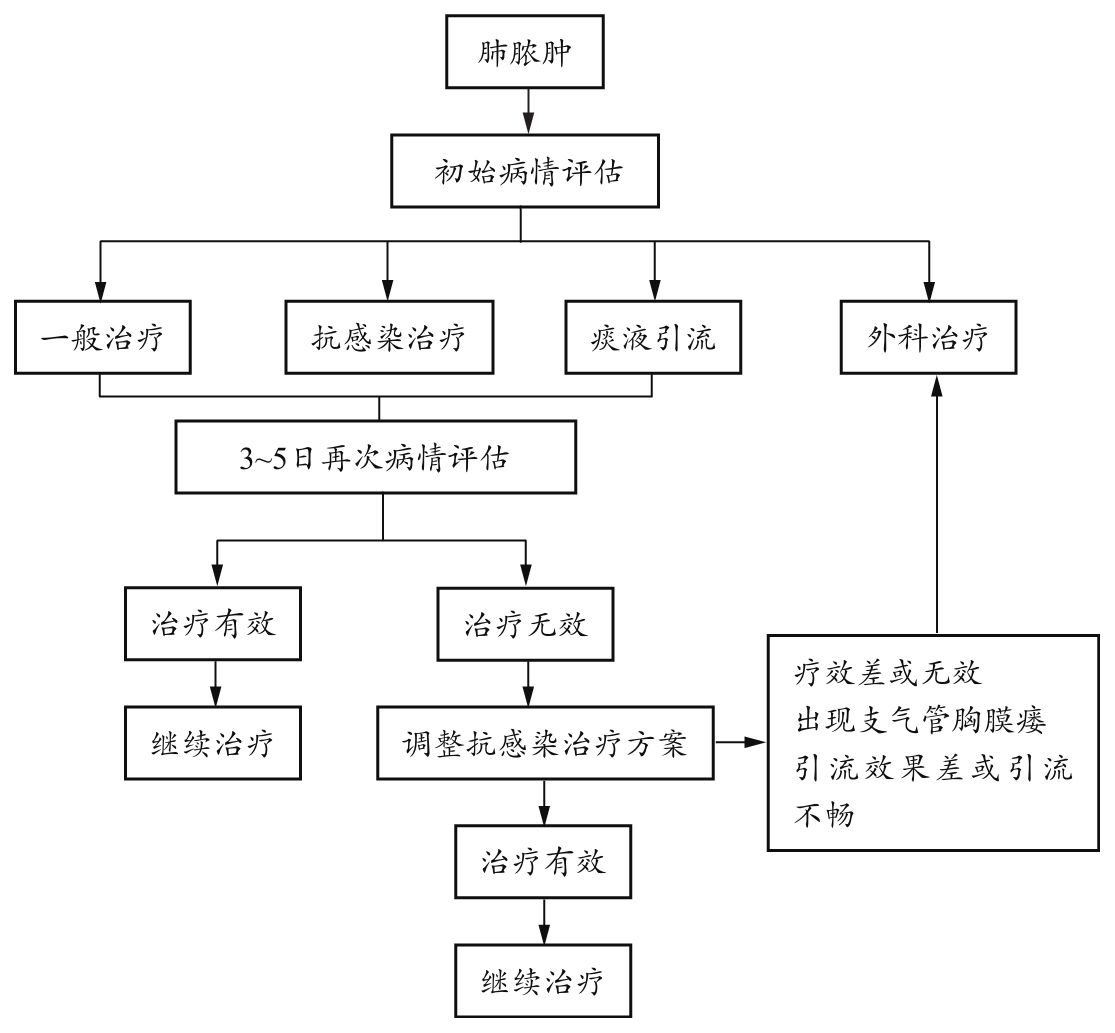
\includegraphics{./images/Image00021.jpg}
 \captionsetup{justification=centering}
 \caption{肺脓肿的治疗程序}
 \label{fig1-9-1}
  \end{figure} 

【治疗方案】

{(一)一般治疗}
 肺脓肿患者一般都有消耗性表现,特别是体质差者,应加强营养治疗,如补液、高营养、高维生素治疗;有缺氧表现者需要吸氧。高热者可进行非甾体类抗炎药退热治疗。

{(二)药物治疗及相关治疗}

1. 抗菌药物治疗

(1)急性肺脓肿的感染细菌包括G{+}
球菌和大多数厌氧菌染,一般均对青霉素敏感,脆弱拟杆菌对青霉素不敏感,但对林可霉素、克林霉素和甲硝唑敏感。可根据病情严重程度决定青霉素剂量,每日剂量为640万\textasciitilde{}1000万U,严重感染者可用2000万U/d,分4次静滴。对厌氧菌感染,除应用青霉素外,尚可选用或联合用其他抗厌氧菌感染治疗,如林可霉素1.8\textasciitilde{}3.0g/d,或克林霉素0.6\textasciitilde{}1.8g/d,或甲硝唑0.4g,每日3次静滴。

(2)如为金黄色葡萄球菌感染,可选用耐β内酰胺酶的青霉素或头孢菌素,如苯唑西林6\textasciitilde{}12g/d;如为MRSA感染,应选用万古霉素、利奈唑胺或替考拉宁。

(3)如为阿米巴原虫感染,则用甲硝唑治疗。

(4)如为革兰阴性杆菌,则可选用第2代或第3代头孢菌素、氟喹诺酮类,可联用氨基糖苷类抗菌药物。

在全身用药基础上,可加用抗生素的局部治疗,如环甲膜穿刺,经鼻导管气道内或经纤维支气管镜滴药,常用青霉素40万\textasciitilde{}80万U,5\textasciitilde{}10ml生理盐水稀释。滴药后按脓肿部位采取适当体位,静卧1小时。

2. 痰液引流 有效的引流排痰可以缩短病程,提高疗效。

(1)可选用祛痰药鲜竹沥10\textasciitilde{}15ml或氨溴索30\textasciitilde{}60mg口服,每日3次,使痰液易咳出。

(2)痰液稠不易咳出者可用雾化吸入生理盐水或氨溴索,以利痰液引流。

(3)身体状况较好、发热不高的患者,可采取体位引流排脓痰,引流的体位应使脓肿处于最高位,轻拍患部,每日2\textasciitilde{}3次,每次10\textasciitilde{}15分钟。

(4)痰液引流不畅者,可经纤维支气管镜冲洗及吸引,并可将抗生素直接滴注到病变部位,每周1\textasciitilde{}2次。

3. 外科治疗 手术治疗适应证为:

(1)肺脓肿病程超过3个月(即慢性肺脓肿),经内科治疗脓腔不缩小,或脓腔过大(6cm以上)估计不易闭合者。

(2)大咯血经内科治疗无效或危及生命。

(3)伴有支气管胸膜瘘或脓胸经抽吸、引流和冲洗疗效不佳者。

(4)支气管阻塞疑为支气管肺癌导致引流不畅的肺脓肿。对病情重不能耐受手术者,可经胸壁插入导管到脓腔进行引流。

术前应评价患者一般情况和肺功能。

【疗效观察与随访】

1. 观察指标

(1)症状、体征:观察咳嗽、咳痰的缓解情况,痰量、痰液性状的变化,伴咯血者其咯血量监测,注意胸闷、气急的好转状况,监测血氧饱和度。注意观察体温,肺实变征的变化等。慢性肺脓肿常有杵状指(趾)。

(2)血常规:可监测血象变化,决定是否继续抗感染治疗。

(3)病原学检查:给予痰和血细菌培养和药敏试验,有条件可经气管吸引或经纤支镜套管防污染毛刷在下呼吸道直接采样,做涂片染色检查和需氧、厌氧菌培养。

(4)胸部X线检查:根据病情需要,可行胸部X线监测肺部脓腔变化,了解病情转归。

2. 治愈标准 症状、体征消失,血象正常,胸部X线摄片病灶消失,无并发症。

3. 随访 注意病情观察,定期胸部摄X线片复查,避免支气管胸膜瘘等并发症。

【治疗经验与解析】

1.
肺脓肿的治疗疗程 抗菌药物疗程6\textasciitilde{}10周,或直至X线胸片脓腔和炎症消失,或仅有少量的残留纤维化。在有效抗生素治疗下,体温一般在治疗3\textasciitilde{}7日下降,7\textasciitilde{}14日可降至正常。3\textasciitilde{}10日内痰恶臭味消失。临床症状改善后,抗生素静脉滴注可改为肌注或口服。

2.
体位引流注意事项 对脓液多而且身体虚弱者应慎重,以免大量脓痰涌出,来不及咳出而造成窒息。

\section{肺血栓栓塞症}

肺血栓栓塞症(pulmonary
thromboembolism,PTE)是肺栓塞的一种类型。肺栓塞(pulmonary
embolism,PE)是以各种栓子阻塞肺动脉系统为其发病原因的一组疾病或临床综合征的总称,包括PTE、脂肪栓塞综合征、羊水栓塞、空气栓塞等。PTE为来自静脉系统或右心的血栓阻塞肺动脉或其分支所致的疾病,以肺循环和呼吸功能障碍为其主要临床和病理生理特征。

PTE为PE最常见的类型,占PE中的绝大多数,通常所称的PE即指PTE。急性PTE造成肺动脉较广泛阻塞时,可引起肺动脉高压,至一定程度导致右心失代偿、右心扩大,出现急性肺源性心脏病。肺动脉发生栓塞后,若其支配区的肺组织因血流受阻或中断而发生坏死,称为肺梗死(pulmonary
infarction,PI)。由于肺组织的多重供血与供氧机制,PTE中仅约不足15\%发生PI。

引起PTE的血栓主要来源于深静脉血栓形成(deep venous
thrombosis,DVT)。DVT与PTE实质上为一种疾病过程在不同部位、不同阶段的表现,两者合称为静脉血栓栓塞症(venous
thromboembolism,VTE)。

PTE和DVT已经构成了世界性的重要医疗保健问题。其发病率较高,病死率亦高。西方国家DVT和PTE的年发病率分别约为1.0‰和0.5‰。新近资料显示,美国VTE的年新发病例数超过60万,其中PTE患者23.7万,DVT患者37.6万,因VTE死亡的病例数超过29万;欧盟国家VTE的年新发病例数超过150万,其中PTE患者43.5万,DVT患者68.4万,因VTE死亡的病例数超过54万。未经治疗的PTE的病死率为25\%\textasciitilde{}30\%。由于PTE-DVT发病和临床表现的隐匿性和复杂性,对PTE-DVT的漏诊率和误诊率普遍较高。

过去我国医学界曾将PTE视为“少见病”,但这种观念近年已发生彻底改变。虽然我国目前尚无准确的流行病学资料,但随着诊断意识和检查技术的提高,诊断例数已有显著增加。尽管如此,由于PTE的发病过程较为隐匿,症状亦缺乏特异性,确诊需特殊的检查技术,使PTE的检出率偏低,临床上仍存在较严重的漏诊和误诊现象,对此应当给予充分关注。

【治疗程序】 图\ref{fig1-10-1}示。

\begin{figure}[!htbp]
 \centering
 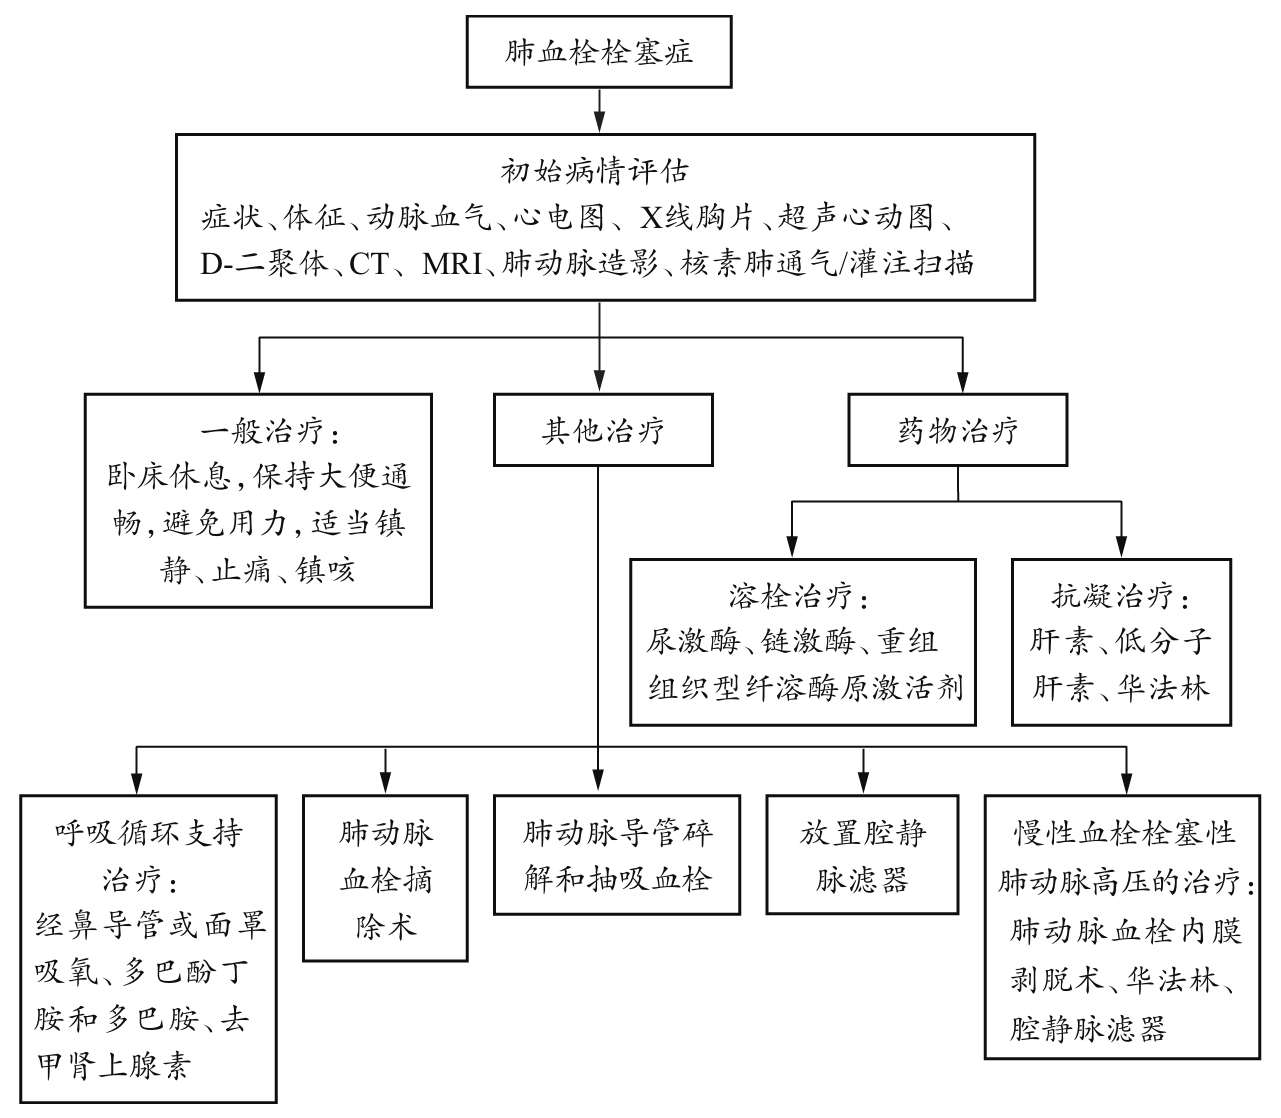
\includegraphics{./images/Image00022.jpg}
 \captionsetup{justification=centering}
 \caption{肺血栓栓塞症的治疗程序}
 \label{fig1-10-1}
  \end{figure} 

【治疗方案】

{(一)一般治疗}
 卧床休息,保持大便通畅,避免用力,以免促进深静脉血栓脱落;可适当使用镇静、止痛、镇咳等相应的对症治疗。

{(二)药物治疗}

1.
溶栓治疗 常用的溶栓药物有尿激酶(UK)、链激酶(SK)和重组组织型纤溶酶原激活剂(rt-PA)。溶栓方案与剂量:

(1)UK:负荷量4400IU/kg,静注10分钟,随后以2200IU/(kg·h)持续静注12小时;另可考虑2小时溶栓方案,按20000IU/kg剂量,持续静注2小时。

(2)SK:负荷量250000IU,静注30分钟,随后以100000IU/小时持续静注24小时。

(3)rt-PA:rt-PA50mg持续静注2小时。

2.
抗凝治疗 抗凝血药物主要有普通肝素(UFH)、低分子肝素(LMWH)和华法林。

(1)普通肝素的推荐用法:予3000\textasciitilde{}5000IU或按80IU/kg静注,继之以18IU/(kg·h)持续静滴。在开始治疗后的最初24小时内每4\textasciitilde{}6小时测定APTT,根据APTT调整剂量,尽快使APTT达到并维持于正常值的1.5\textasciitilde{}2.5倍。达稳定治疗水平后,改为每日测定APTT一次。肝素亦可用皮下注射方式给药。一般先予静注负荷量300\textasciitilde{}5000IU,然后按250IU/kg剂量每12小时皮下注射一次。调节注射剂量,使注射后6\textasciitilde{}8小时的APTT达到治疗水平。

(2)低分子肝素的用法:现在有多种制剂供临床选用,一般根据体重给药。如低分子肝素钠2500\textasciitilde{}5000U皮下注射,12小时一次,或者100U/kg皮下注射,每日2次。

(3)华法林:在肝素开始应用后的第1\textasciitilde{}3日加用口服抗凝剂华法林,初始剂量为3.0\textasciitilde{}5.0mg/d。由于华法林需要数日才能发挥全部作用,因此与肝素需至少重叠应用4\textasciitilde{}5日,当连续两日测定的国际标准化比率(INR)达到2.5(2.0\textasciitilde{}3.0)时,或PT延长至正常值的1.5\textasciitilde{}2.5倍时,方可停止使用肝素,单独口服华法林治疗。应根据INR或PT调节华法林的剂量。

{(三)其他治疗}

1.
呼吸循环支持治疗 采用经鼻导管或面罩吸氧,以纠正低氧血症。对于出现右心功能不全但血压正常者,可使用多巴酚丁胺和多巴胺;若出现血压下降,可增大剂量或使用其他血管加压药物,如去甲肾上腺素等。

2.
肺动脉血栓摘除术 风险大,病死率高,需要较高的技术条件,仅适用于经积极的内科治疗无效的紧急情况,如致命性肺动脉主干或主要分支堵塞的大面积PTE,或有溶栓禁忌证者。

3.
肺动脉导管碎解和抽吸血栓 用导管碎解和抽吸肺动脉内巨大血栓,同时还可进行局部小剂量溶栓。适应证为肺动脉主干或主要分支的大面积PTE,并存在以下情况者:溶栓和抗凝治疗禁忌;经溶栓或积极的内科治疗无效;缺乏手术条件。

4.
放置腔静脉滤器 为防止下肢深静脉大块血栓再次脱落阻塞肺动脉,可考虑放置下腔静脉滤器。对于上肢DVT病例,还可应用上腔静脉滤器。置入滤器后如无禁忌证,宜长期口服华法林抗凝,定期复查有无滤器上血栓形成。

5.
慢性血栓栓塞性肺动脉高压(CTEPH)的治疗 若阻塞部位处于手术可及的肺动脉近端,可考虑行肺动脉血栓内膜剥脱术;口服华法林3.0\textasciitilde{}5.0mg/d,根据INR调整剂量,保持INR为2.0\textasciitilde{}3.0;反复下肢深静脉血栓脱落者,可放置下腔静脉滤器。

【疗效观察与随访】

1. 观察指标

(1)一般项目:应进行严密监护,监测呼吸、心率、血压、静脉压、心电图及动脉血气的变化。

(2)溶栓治疗:应每2\textasciitilde{}4小时测定凝血酶原时间(PT)或活化部分凝血酶原时间(APTT)。

(3)抗凝治疗:应用肝素或低分子肝素前应测定基础APTT、PT及血常规(含血小板计数,血红蛋白)。因肝素可能会引起血小板减少症(HIT),在使用肝素的第3\textasciitilde{}5日必须复查血小板计数。若较长时间使用肝素,尚应在第7\textasciitilde{}10日复查。使用华法林在达到治疗水平前,应每日测定国际标准化比率(INR),其后2周每周监测2\textasciitilde{}3次,以后根据INR的稳定情况每周监测1次或更少。

2.
治愈标准 症状、体征消失,急诊状态解除,相关检测指标恢复正常,2周内未复发。

3.
随访 注意病情观察,特别是华法林长期治疗者,约每4周测定INR并调整华法林剂量1次,避免不良反应。

【治疗经验与解析】

1. 溶栓治疗

(1)临床应用:主要适用于大面积PTE病例(有明显呼吸困难、胸痛、低氧血症等)对于次大面积PTE,若无禁忌证也可考虑溶栓,但存在争议;对于血压和右心室运动功能均正常的病例,不宜溶栓。溶栓的时间窗一般定为14日以内,但若近期有新发PTE征象可适当延长。溶栓应尽可能在PTE确诊的前提下慎重进行。对有明确溶栓指征的病例宜尽早开始溶栓。

(2)溶栓治疗的主要并发症:出血。最严重的是颅内出血,发生率1\%\textasciitilde{}2\%,发生者近半数死亡。用药前应充分评估出血的危险性,必要时应配血,做好输血准备。溶栓前宜留置外周静脉套管针,以方便溶栓中取血监测,避免反复穿刺血管。

(3)溶栓治疗的禁忌证:绝对禁忌证有活动性内出血和近期自发性颅内出血。相对禁忌证有2周内的大手术、分娩、器官活检或不能压迫止血部位的血管穿刺;2个月内的缺血性脑卒中;10日内的胃肠道出血;15日内的严重创伤;1个月内的神经外科或眼科手术;难于控制的重度高血压(收缩压\textgreater{}180mmHg,舒张压\textgreater{}110mmHg);近期曾行心肺复苏;血小板计数\textless{}100×10$^{9}$
/L;妊娠;细菌性心内膜炎;严重肝、肾功能不全;糖尿病出血性视网膜病变等。对于致命性大面积PTE,上述绝对禁忌证亦应被视为相对禁忌证。

(4)链激酶:具有抗原性,故用药前需肌注苯海拉明或地塞米松,以防止过敏反应。链激酶6个月内不宜再次使用。使用尿激酶、链激酶溶栓时无须同时使用肝素治疗;但以rt-PA溶栓,当rt-PA注射结束后,应继续使用肝素。用尿激酶或链激酶溶栓治疗后,应每2\textasciitilde{}4小时测定一次凝血酶原时间(PT)或活化部分凝血活酶时间(APTT),当其水平降至正常值的2倍时,即应启动规范的肝素治疗。溶栓后应注意对临床及相关辅助检查情况进行动态观察,评估溶栓疗效。国内多中心研究结果提示rt-PA
50mg持续静脉滴注2小时已经取得理想的溶栓效果,而将rt-PA增加到100mg并未能提高溶栓治疗的有效率,这与欧美的研究结果不同,因此推荐rt-PA
50mg持续静注2小时为国人标准治疗方案。

2.
肝素抗凝治疗要点 抗凝治疗为PTE和DVT的基本治疗方法,可以有效的防止血栓再形成和复发,为机体发挥自身的纤溶机制溶解血栓创造条件。

抗血小板药物的抗凝作用不能满足PTE或DVT的抗凝要求。临床疑诊PTE时,即可开始使用UFH或LMWH进行有效的抗凝治疗。

应用UFH/LMWH前应测定基础APTT、PT及血常规(含血小板计数、血红蛋白);应注意是否存在抗凝的禁忌证,如活动性出血、凝血功能障碍、未予控制的严重高血压等。对于确诊的PTE病例,大部分禁忌证属相对禁忌证。

因可能会引起肝素诱导的血小板减少症(HIT),在使用UFH时,第1周每1\textasciitilde{}2日、第2周起每3\textasciitilde{}4日必须复查血小板计数一次。若出现血小板迅速或持续降低达30\%以上,或血小板计数\textless{}100×10$^{9}$
/L,应停用UFH。一般在停用肝素后10日内血小板开始逐渐恢复。需注意HIT可能会伴发PTE和DVT的进展或复发。当血栓复发的风险很大而又必须停用肝素时,可考虑放置下腔静脉滤器,但需警惕滤器处合并腔静脉血栓。

使用低分子肝素不需监测APTT和调整剂量,使用较普通肝素方便而且疗效好。

UFH或LMWH须至少应用5日,直到临床情况平稳。对大面积PTE或髂股静脉血栓,UFH或LMWH须用至10日或更长。

抗凝治疗的持续时间因人而异。一般口服华法林的疗程至少为3\textasciitilde{}6个月。部分病例的危险因素短期可以消除,例如服雌激素或临时制动,疗程可能为3个月即可;对于栓子来源不明的首发病例,需至少给予6个月的抗凝;对复发性VTE、并发肺心病或危险因素长期存在者,抗凝治疗的时间应更为延长,达12个月或以上,甚至终身抗凝。

3.
妊娠的前3个月和最后6周禁用华法林,可用肝素或低分子肝素治疗。产后和哺乳期妇女可以服用华法林。华法林的主要并发症是出血。华法林所致出血可以用维生素K拮抗。华法林有可能引起血管性紫癜,导致皮肤坏死,多发生于治疗的前几周。

\section{肺结核病}

肺结核病(pulmonary tuberculosis)是结核分枝杆菌(mycobacterium
tuberculosis,简称结核杆菌或结核菌)引起的慢性肺部感染性疾病,占各器官结核病总数的80\%\textasciitilde{}90\%,其中痰中排菌者称为传染性非结核病。在21世纪仍然是严重危害人类健康的主要传染病,是全球关注的公共卫生和社会问题,也是我国重点控制的主要疾病之一。

【治疗程序】 图\ref{fig1-11-1}所示。

\begin{figure}[!htbp]
 \centering
 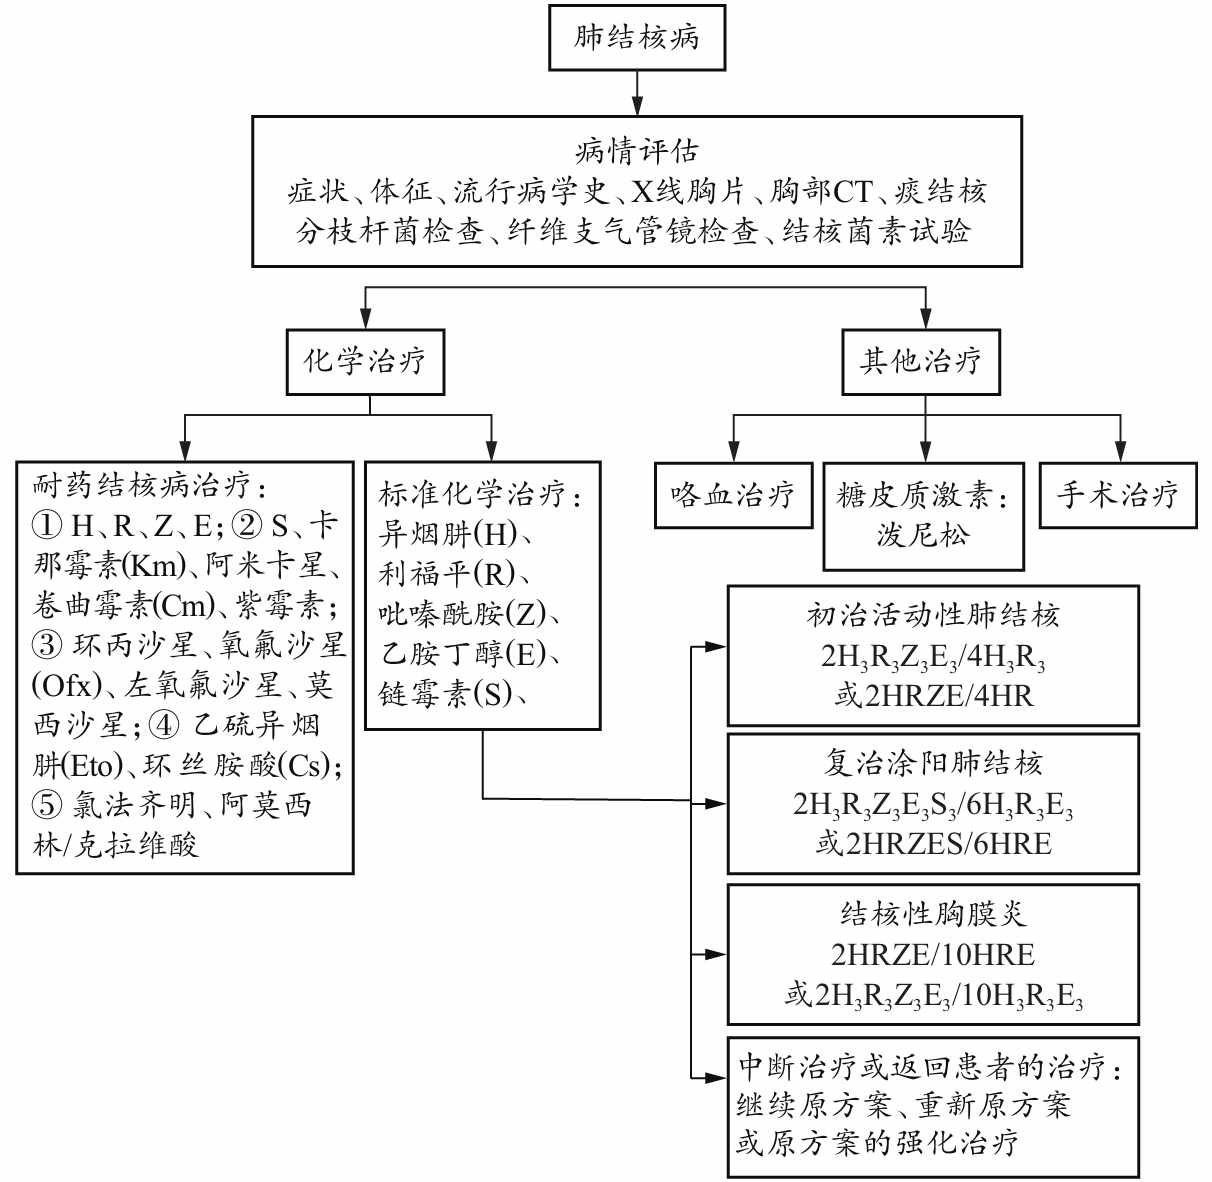
\includegraphics{./images/Image00023.jpg}
 \captionsetup{justification=centering}
 \caption{肺结核病的治疗程序}
 \label{fig1-11-1}
  \end{figure} 

【治疗方案】

{(一)治疗原则}
 化学疗法是肺结核病的基本治疗,早期、联合、规律、全程、适量是肺结核病化疗的原则,以期达到消灭结核菌、治愈疾病、防止耐药菌产生、减少复发的目的。

{(二)一般治疗}
 注意休息、隔离,避免精神紧张。发热、盗汗等症状一般无需治疗,高热时给予糖皮质激素、非甾体类消炎药对症治疗。

{(三)常用抗结核病药物}

1. 异烟肼(isoniazid,INH,H) 片剂,每片0.1g,特制每片0.3g。

2. 利福平(rifampicin,RFP,R) 胶囊剂,每粒0.15g,特制每粒0.3g。

3. 利福喷汀(rifapentine,RFT) 胶囊剂,每粒0.15g。

4. 吡嗪酰胺(pyrazinamide,PZA,Z) 片剂,每片0.25g,特制每片0.5g。

5. 乙胺丁醇(ethambutol,EMB,E) 片剂,每片0.25g。

6. 链霉素(streptomycin,SM,S) 注射剂(硫酸盐),每支0.75g。

{(四)抗结核药物用量与用法(表\ref{tab1-11-1})。}

\begin{table}[htbp]
\centering
\caption{不同疗法中常用抗结核药物的用量与用法}
\label{tab1-11-1}
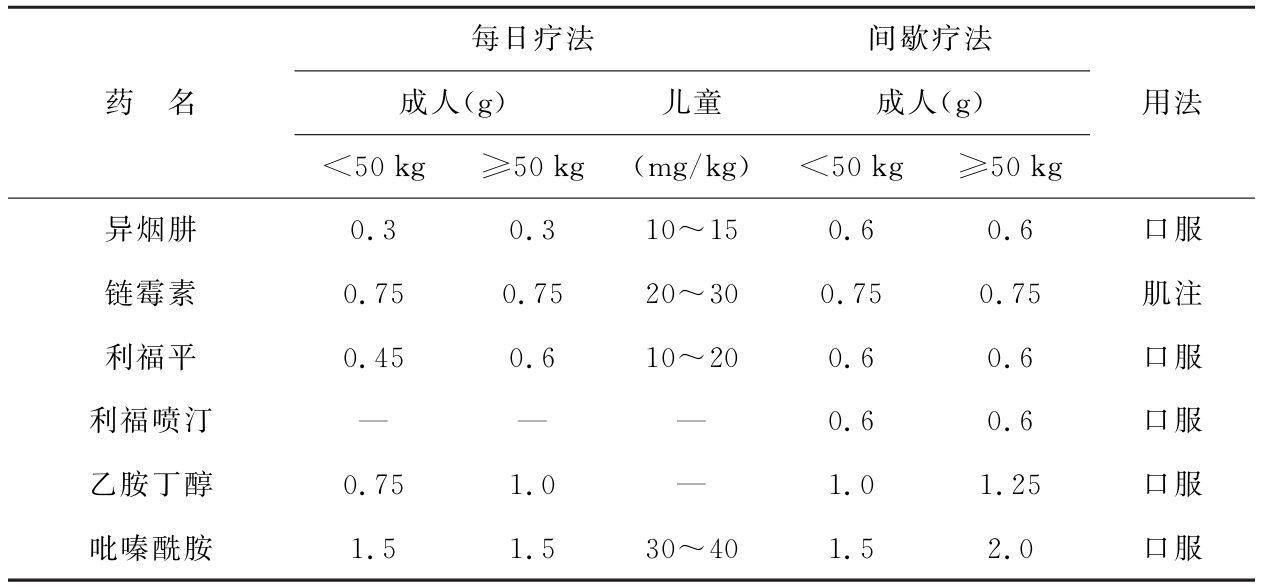
\includegraphics{./images/Image00024.jpg}
\end{table}

{(五)统一标准化学治疗方案}

1.
初治活动性肺结核化疗方案 新涂阳和新涂阴肺结核患者可选用以下方案治疗。

(1)间歇用药方案:①强化期:异烟肼、利福平、吡嗪酰胺和乙胺丁醇,隔日1次,共2个月,用药30次。②继续期:异烟肼、利福平,隔日1次,共4个月,用药60次。全疗程共计90次。简写为2H{3}
R{3} Z{3} E{3} /4H{3} R{3}
(药名前数字表示用药月数,药名右下方数字表示每周用药次数)。

(2)每日用药方案:①强化期:异烟肼、利福平、吡嗪酰胺和乙胺丁醇,每日1次,共2个月,用药60次。②继续期:异烟肼、利福平,每日1次,共4个月,用药120次。全疗程共计180次。简写为2HRZE/4HR。

2. 复治涂阳肺结核治疗方案

(1)间歇用药方案:①强化期:异烟肼、利福平、吡嗪酰胺、链霉素和乙胺丁醇,隔日1次,共2个月。②继续期:异烟肼、利福平和乙胺丁醇,隔日1次,共6个月,用药90次。全疗程共计120次。简写为2H{3}
R{3} Z{3} E{3} S{3} /6H{3} R{3} E{3} 。

(2)每日用药方案:①强化期:异烟肼、利福平、吡嗪酰胺、链霉素和乙胺丁醇,每日1次,共2个月。②继续期:异烟肼、利福平和乙胺丁醇,每日1次,共6个月,用药180次。全疗程共计240次。简写为2HRZES/6HRE。

3. 结核性胸膜炎治疗方案

(1)每日用药方案:①强化期:异烟肼、利福平、吡嗪酰胺和乙胺丁醇,每日1次,共2个月,用药60次。②继续期:异烟肼、利福平和乙胺丁醇,每日1次,共10个月,用药300次。全疗程共计360次。简写为2HRZE/10HRE。

(2)间歇用药方案:①强化期:异烟肼、利福平、吡嗪酰胺和乙胺丁醇,隔日1次,共2个月,用药30次。②继续期:异烟肼、利福平和乙胺丁醇,隔日1次,共10个月,用药150次。全疗程共计180次。简写为2H{3}
R{3} Z{3} E{3} /10H{3} R{3} E{3} 。

4. 中断治疗或返回患者的治疗

(1)初治活动性肺结核患者(包括结核性胸膜炎)中断治疗后的继续治疗(表\ref{tab1-11-2}\footnote{所有患者必须完成2个月的强化期治疗。如果患者中断治疗前已完成1个月的强化期治疗,将再给他不少于1个月的强化期治疗,而后才开始继续期治疗}\footnote{即从头开始初治方案,已完成的治疗不计在内})。

\begin{table}[htbp]
\centering
\caption{中断治疗\textless{}2个月的初治活动性肺结核患者的治疗}
\label{tab1-11-2}
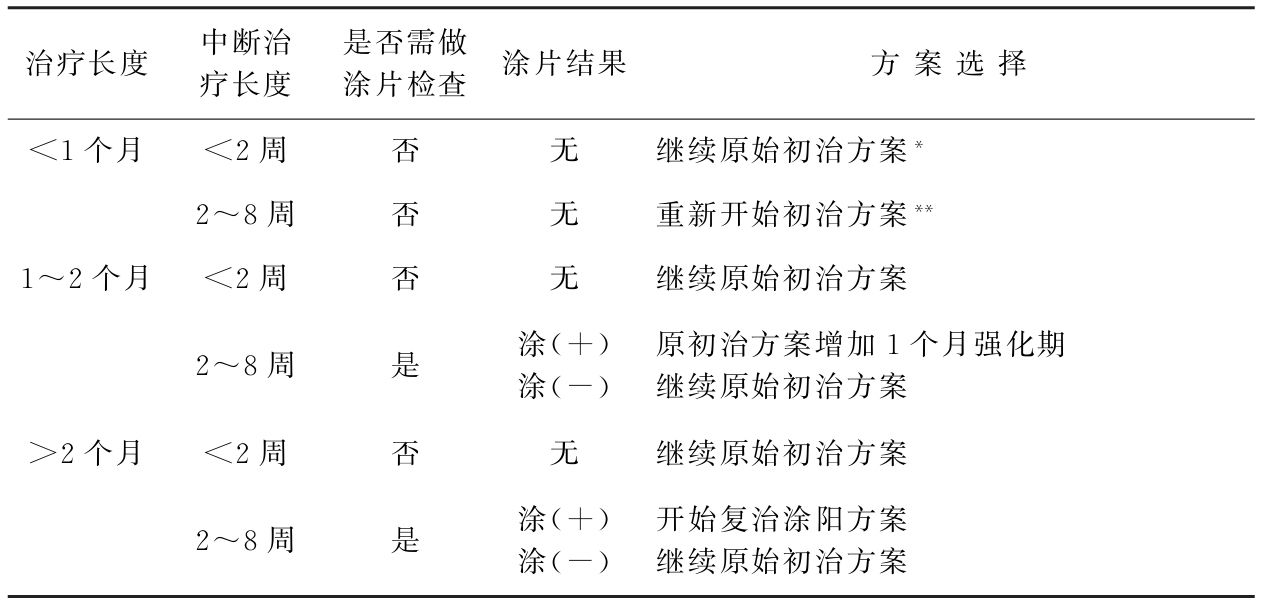
\includegraphics{./images/Image00025.jpg}
\end{table}

(2)复治涂阳肺结核患者中断治疗后的继续治疗(表\ref{tab1-11-3}\footnote{保证患者完成2个月的强化期治疗})。

\begin{table}[htbp]
\centering
\caption{中断治疗\textless{}2个月的复治涂阳肺结核患者的治疗}
\label{tab1-11-3}
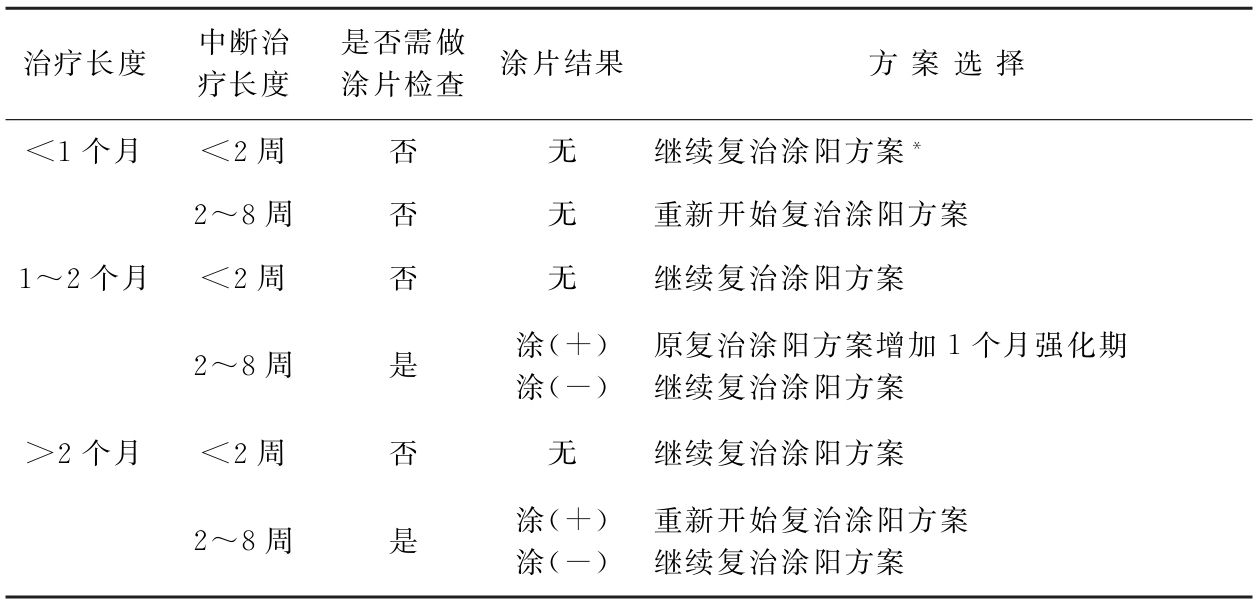
\includegraphics{./images/Image00026.jpg}
\end{table}

{(六)耐药肺结核}  耐多药结核病(multidrug resistant
tuberculosis,MDR-TB)治疗方案通常含2个阶段:强化期(注射剂使用)和继续期(注射剂停用),治疗方案采用标准代码,例如6Z-Km(Cm)-Ofx-Eto-Cs/12Z-Ofx-Eto-Cs,初始强化期含5种药,治疗6个月,注射剂停用后,口服药持续至少12个月,总疗期18个月。注射剂为卡那霉素(Km),也可选择卷曲霉素(Cm)。

{(七)其他治疗}

1.
咯血治疗 咯血是肺结核的常见症状,在活动性和痰涂阳肺结核患者中,咯血症状分别占30\%和40\%。咯血处置要注意镇静、止血,患侧卧位,预防和抢救因咯血所致的窒息并防止肺结核播散。

一般少量咯血,多以安慰患者、消除紧张、卧床休息为主,可用氨基己酸、氨甲苯酸(止血芳酸)、酚磺乙胺(止血敏)、卡络柳钠(安络血)等药物止血。大咯血时先用垂体后叶素5\textasciitilde{}10U加入25\%葡萄糖液40ml中缓慢静脉注射,一般为15\textasciitilde{}20分钟,然后将垂体后叶素加入5\%葡萄糖液按0.1U/(kg·h)速度静脉滴注。垂体后叶素收缩小动脉,使肺循环血量减少而达到较好止血效果。高血压、冠状动脉粥样硬化性心脏病、心力衰竭患者和孕妇禁用。对支气管动脉破坏造成的大咯血可采用支气管动脉栓塞法。在大咯血时,患者突然停止咯血,并出现呼吸急促、面色苍白、口唇发绀、烦躁不安等症状时,常为咯血窒息,应及时抢救。置患者头低足高45°的俯卧位,同时拍击健侧背部,保持充分体位引流,尽快使积血和血块由气管排出,或直接刺激咽部以咳出血块。有条件时可进行气管插管,硬质支气管镜吸引或气管切开。

2.
糖皮质激素 在结核病的应用主要是利用其抗炎、抗毒作用。仅用于结核毒性症状严重者。必须确保在有效抗结核药物治疗的情况下使用。使用剂量依病情而定,一般用泼尼松口服每日20mg,顿服,1\textasciitilde{}2周,以后每周递减5mg,用药时间为4\textasciitilde{}8周。

3.
肺结核外科手术治疗 当前肺结核外科手术治疗主要的适应证是经合理化学治疗后无效、多重耐药的厚壁空洞、大块干酪灶、结核性脓胸、支气管胸膜瘘和大咯血保守治疗无效者。

【疗效观察与随访】

1. 观察指标 常见症状、体征、血象、血沉、病原学检查、胸部X线摄片等。

(1)观察患者的症状、体征变化,注意咯血的转归。

(2)初治涂阳、涂阴肺结核患者在治疗至第2个月末、5个月末和疗程末(6个月末);复治涂阳肺结核患者在治疗至第2个月末、5个月末和疗程末(8个月末)要分别收集晨痰和夜间痰各1份进行涂片检查。初、复治涂阳肺结核患者在治疗第2个月末,痰菌仍为阳性者,应在治疗第3个月末增加痰涂片检查一次。确诊并登记的涂阴肺结核患者,即使患者因故未接受治疗,也应在登记后满2个月和满6个月时进行痰菌检查。

2.
治愈标准 症状、体征消失,血沉恢复至正常范围,痰找结核菌2次以上阴性,胸部X线摄片病灶完全吸收或已钙化。

3. 随访

(1)治疗过程中出现恶心、呕吐、厌油、肝区疼痛等肝脏损伤症状以及其他不良反应者,进行肝功能等相应检查。

(2)治疗后1个月查血常规、尿常规、心电图各1次观察不良反应,治疗结束进行X线胸片以帮助判定治疗效果。

【治疗经验与解析】

1.
初治活动性肺结核化疗方案要点 ①如新涂阳肺结核患者治疗到2个月末痰菌检查仍为阳性,则应延长1个月的强化期治疗,继续期化疗方案不变,第3个月末增加1次查痰;如第5个月末痰菌阴性则方案为3H{3}
R{3} Z{3} E{3} /4H{3} R{3}
或3HRZE/4HR。在治疗到第5个月末或疗程结束时痰涂片仍阳性者,为初治失败。②如新涂阴肺结核患者治疗过程中任何一次痰菌检查阳性,均为初治失败。③所有初治失败患者均应进行重新登记,分类为“初治失败”,用复治涂阳肺结核化疗方案治疗。④儿童慎用乙胺丁醇。⑤对初治失败的患者,如有条件可增加痰培养和药敏试验,根据药敏试验结果制定化疗方案。

2.
复治涂阳肺结核治疗方案要点 ①因故不能用链霉素的患者,延长1个月的强化期即3H{3}
R{3} Z{3} E{3} /6H{3} R{3} E{3}
或3HRZE/6HRE。②如复治涂阳肺结核患者治疗到第2个月末痰菌仍阳性,使用链霉素方案治疗的患者则应延长1个月的复治强化期方案治疗,继续期治疗方案不变,即3H{3}
R{3} Z{3} E{3} S{3} /6H{3} R{3} E{3}
或3HRZES/6HRE;未使用链霉素方案的患者则应再延长1个月的强化期,继续期治疗方案不变,即4H{3}
R{3} Z{3} E{3} /6H{3} R{3} E{3}
或4HRZE/6HRE,均应在第3个月末增加1次查痰。第5个月末或疗程结束时痰菌阳性为复治失败。③复治涂阳肺结核患者复治失败,不再为其提供免费治疗。④在有条件的地区,对复治失败的患者,可增加痰培养和药敏试验,根据药敏试验结果制定化疗方案。

3.
肺结核患者的治疗管理方式要点 肺结核患者的治疗管理方式有全程督导化疗、强化期督导化疗、全程管理和自服药。

(1)全程督导化疗:指在肺结核患者的治疗全过程中,患者每次用药均在督导人员直接面视下进行。涂阳患者和含有粟粒、空洞的新涂阴患者应采用全程督导化疗的治疗管理方式。

(2)强化期督导:指在肺结核患者治疗强化期内,患者每次用药均在督导人员直接面视下进行,继续期采用全程管理。非粟粒、空洞的新涂阴肺结核以及结核性胸膜炎患者应采用强化期督导的治疗管理方式。

(3)全程管理:指在肺结核患者治疗全过程中,通过对患者加强宣教,定期门诊取药,家庭访视,复核患者服药情况(核查剩余药品量、尿液抽检等),误期(未复诊或未取药)追回等综合性管理方法,以保证患者规则用药。具体做法为:①做好对肺结核患者初诊的宣教,内容包括解释病情,介绍治疗方案,药物剂量、用法和不良反应以及坚持规则用药的重要性;②定期门诊取药,建立统一的取药记录,强化期每2周或1个月取药1次,继续期每月取药1次。凡误期取药者,应及时通过电话、家庭访视等方式追回患者,并加强教育,说服患者坚持按时治疗。对误期者城镇要求在3日内追回,农村在5日内追回;③培训患者和家庭成员,使其能识别抗结核药物,了解常用剂量和用药方法,以及可能发生的不良反应,并督促患者规则用药;④全程管理也应使用“肺结核患者治疗记录卡”,由患者及家庭成员填写;⑤家庭访视:建立统一的访视记录,村卫生室(社区卫生服务站)医生接到新的治疗患者报告后应尽早做家庭访视,市区1周内,郊区10日内进行初访,化疗开始后至少每月家庭访视1次。内容包括健康教育,核实服药情况,核查剩余药品量,抽查尿液,督促患者按期门诊取药和复查等;⑥做好痰结核菌的定期检查工作,治疗期间按规定时间送痰标本进行复查。

\section{支气管扩张症}

支气管扩张症(bronchiectasis)多见于儿童和青年。是支气管肺组织感染和支气管阻塞,大多继发于急、慢性呼吸道感染和支气管阻塞后,反复发生支气管炎症,致使支气管壁结构破坏,引起支气管异常和持久性扩张。扩张的支气管包括三种不同类型。①柱状扩张:支气管呈均一管形扩张且突然在一处变细,远处的小气道往往被分泌物阻塞。②囊状扩张:扩张的支气管腔呈囊状改变,支气管末端的盲端也呈无法辨认的囊状结构。③不规则扩张:病变支气管腔呈不规则改变或呈串珠样改变。显微镜下可见支气管炎症及纤维化、支气管壁溃疡、鳞状上皮化生和粘液腺增生。临床表现主要为慢性咳嗽、咳大量脓痰和(或)反复咯血。近年来随着急、慢性呼吸道感染的恰当治疗,其发病率有减少趋势。

【治疗程序】 图\ref{fig1-12-1}所示。

\begin{figure}[!htbp]
 \centering
 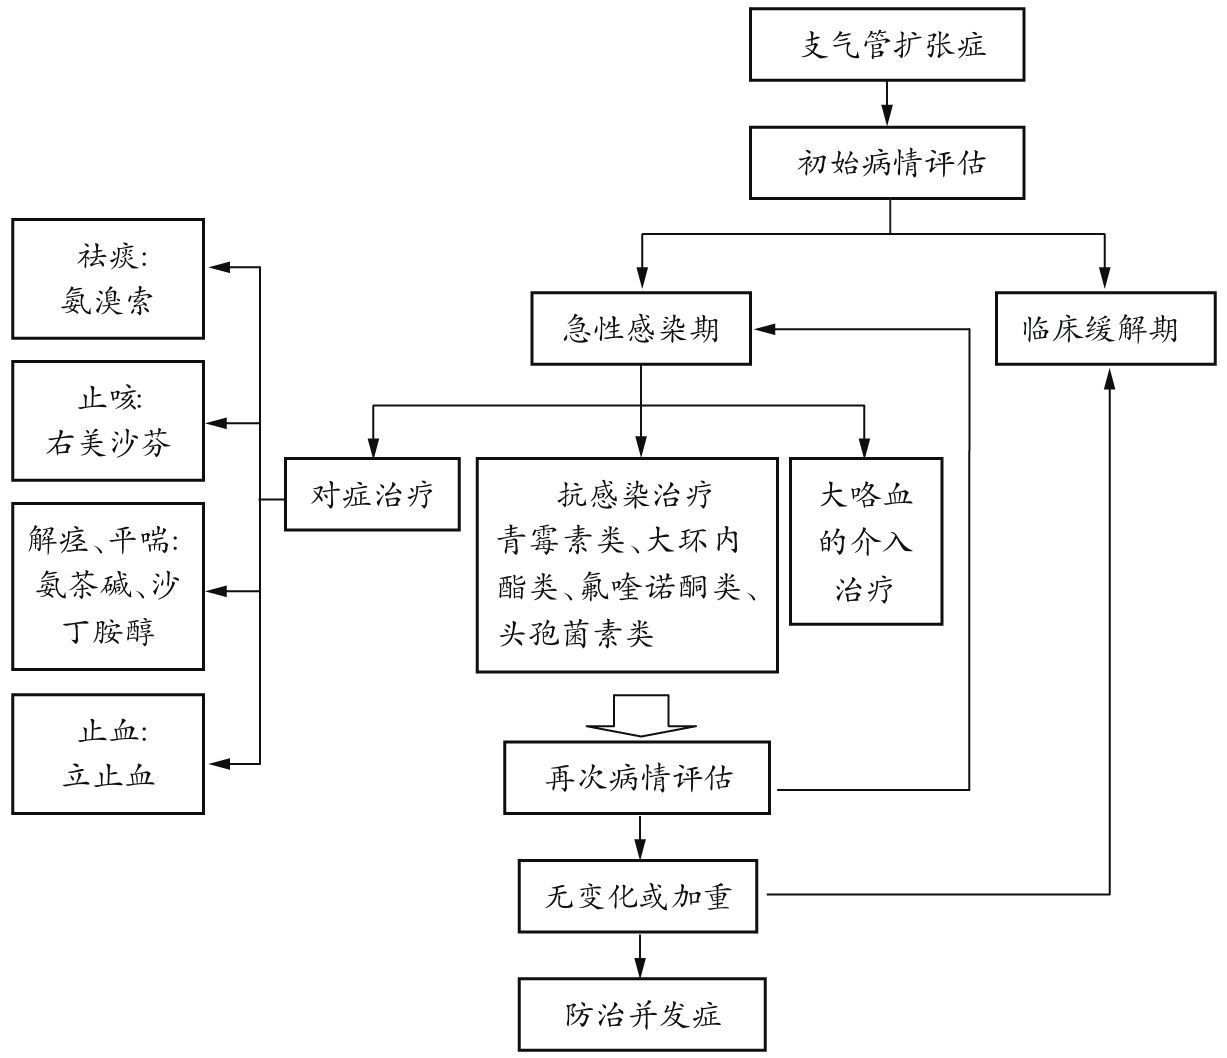
\includegraphics{./images/Image00027.jpg}
 \captionsetup{justification=centering}
 \caption{支气管扩张症的治疗程序}
 \label{fig1-12-1}
  \end{figure} 

【治疗方案】

{(一)治疗目的和治疗原则}

1.
治疗目的 支气管扩张症,其解剖学上的损害为不可逆,治疗目的是防止病情进展,控制症状。

2. 治疗原则 去除病原菌,促进痰液排除,控制感染,必要时手术切除。

{(二)一般治疗}  注意休息、保暖,多饮水。

{(三)药物治疗}

1. 保持呼吸道引流通畅

(1)祛痰、止咳治疗:保持体液平衡可以使痰液变稀薄,有利于粘痰排出。常用祛痰药有溴己新、乙酰半胱氨酸、氨溴索等,并可酌情应用右美沙芬、咳必清等镇咳剂,如咳必清25mg口服,每日3次。

(2)体位引流:是根据病变部位采取不同的体位,原则上应使患肺处于高位,引流支气管开口朝下,以利于痰液流入大支气管和气管排出。每日2\textasciitilde{}4次,每次15\textasciitilde{}30分钟。体位引流时,间歇做深呼吸后用力咳痰,同时旁人协助用手轻拍患部,可提高引流效果。

(3)支气管扩张剂治疗:部分病例由于支气管反应性增高或炎症的刺激,可出现支气管痉挛,影响痰液排出。在不咯血情况下,可以酌情应用茶碱制剂,必要时可加用支气管扩张剂雾化吸入治疗(如β{2}
受体激动剂或异丙托溴铵)。

(4)气管镜吸痰:如经过上述处理后痰仍难以排出,可依据病情考虑使用气管镜吸痰,及用生理盐水冲洗稀释痰液。

2.
控制感染 是支气管扩张急性感染期的主要治疗措施。应根据症状、体征、痰液性状,和痰液革兰染色和痰培养结果指导抗生素应用,但在开始时常需给予经验治疗(如给予氨苄西林、阿莫西林或头孢克洛)。存在铜绿假单胞菌感染时,可选择第3代或第4代头孢菌素,有循证医学的研究发现第4代头孢菌素(头孢吡肟)抗铜绿假单胞菌疗效更优,并可联合大环内酯类,因为大环内酯类药物可以破坏铜绿假单胞菌的生物被膜,使头孢菌素类药物更易杀死铜绿假单胞菌。对于慢性咯脓痰的患者,除使用短程抗生素外,还可考虑使用疗程更长的抗生素,如口服阿莫西林或吸入氨基糖苷类,或间断并规则使用单一抗生素以及轮换使用抗生素。

{(四)咯血的处理}

(1)一般少量咯血:多以对症处理为主,包括安慰患者、消除紧张、卧床休息,可用氨基己酸、氨甲苯酸(止血芳酸)、酚磺乙胺(止血敏)、卡巴克洛(安络血)等药物止血。年老体衰、肺功能不全者,慎用强镇咳药物,以免因抑制咳嗽反射及呼吸中枢,使血块不能排出而引起窒息。

(2)中等或大咯血时:应严格卧床休息,胸部放置冰袋,并配血备用。取患侧卧位,轻轻将存留在气管内的积血咳出。可用垂体后叶素5\textasciitilde{}10U加入25\%葡萄糖液40ml中缓慢静脉注射,一般为15\textasciitilde{}20分钟,然后将垂体后叶素加入5\%葡萄糖液按0.1U/(kg·h)速度静脉滴注。垂体后叶素收缩小动脉,使肺循环血量减少而达到较好止血效果。高血压、冠状动脉粥样硬化性心脏病、心力衰竭患者和孕妇禁用。

(3)在大咯血时:患者突然停止咯血,并出现呼吸急促、面色苍白、口唇发绀、烦躁不安等症状时,常为咯血窒息,应及时抢救。置患者头低足高45°的俯卧位,同时拍击健侧背部,保持充分体位引流,尽快使积血和血块由气管排出,或直接刺激咽部以咳出血块。有条件时可进行气管插管,硬质支气管镜吸引或气管切开。

若有中等量以上的咯血,经过内科治疗未能控制,可进行支气管动脉造影,对出血动脉定位,进行动脉栓塞治疗。

{(五)外科治疗}
 如果支气管扩张为局限性,且经充分的内科治疗仍顽固反复发作者,可考虑外科手术切除病变肺组织。如果大出血来自于增生的支气管动脉、经休息和抗生素等保守治疗不能缓解反复大咯血时,病变局限者可考虑外科手术,否则采用支气管动脉栓塞术治疗。对于那些尽管采取了所有治疗仍致残的病例,合适者可考虑肺移植。

【疗效观察与随访】

1. 观察指标

(1)症状、体征:观察咳嗽、咳痰的缓解情况,痰量、痰液性状,以及胸闷、气急的程度。监测体温、两肺呼吸音以及啰音的变化等。

(2)血常规:可根据血象变化,决定下一步治疗方案。

(3)病原学检查:痰涂片、痰培养及药敏试验,有助于指导治疗。

2. 好转标准 症状显著减轻,感染已控制,胸部X线摄片病情稳定。

3.
随访 注意病情观察,观察症状、体征等变化,避免致病因素,避免合并症、并发症。

【治疗经验与解析】

1.
急性感染期的治疗应以控制感染和祛痰、排痰为主;伴发喘息时,应予解痉平喘治疗。对老年体弱无力咳痰者或痰量较多者,应以祛痰为主,不宜选用强镇咳药,如可待因,以免抑制呼吸中枢及加重呼吸道阻塞,导致病情恶化。

2. 咯血窒息是支气管扩张咯血致死的最主要原因,需严加防范,积极抢救。

3.
临床缓解期应注意避免各种致病因素,吸烟者需要戒烟。特别是需要化痰药物,以及振动、拍背和体位引流等胸部物理治疗,均有助于清除气道分泌物;同时加强锻炼、增强体质,预防感染。

\section{原发性支气管肺癌}

原发性支气管肺癌(primary bronchogenic carcinoma)简称肺癌(lung
cancer),起源于支气管粘膜或腺体,是最常见的肺部原发性恶性肿瘤。肺癌的发病机制迄今未完全明确,但有证据显示与吸烟、空气污染、职业致癌因子、电离辐射、饮食与营养及遗传因素等有关。按解剖学部位肺癌分为中央型及周围型,按组织病理学可分为两大类,即小细胞肺癌(small
cell lung cancer,SCLC)和非小细胞肺癌(nonsmall cell lung
cancer,NSCLC),后者包括鳞状细胞癌、腺癌、大细胞肺癌及腺癌混杂亚型等。其临床表现与肺癌的发生部位、类型、大小、有无转移和并发症等有关。诊断主要依靠X线、CT等影像学检查及痰脱落细胞学检查、纤支镜等,病理学检查对其诊断有决定性意义。

【治疗程序】 图\ref{tab1-13-1}\footnote{任何大小的非常见的表浅播散的肿瘤,只要其浸润成分局限于支气管壁,即使临近主支气管,也定义为T1。}
\footnote{肿瘤≤5cm或者大小无法确定的T2肿瘤定义为T2a,肿瘤\textgreater{}5cm但≤7cm的T2肿瘤定义为T2b。}
\footnote{大多数肺癌患者的胸腔积液(以及心包积液)由肿瘤引起。但是有极少数患者的胸腔积液(心包积液)多次细胞学检查肿瘤细胞均呈阴性,且积液为非血性液,亦非渗出液。如综合考虑这些因素并结合临床确定积液与肿瘤无关时,积液将不作为分期依据,患者仍按T1、T2、T3或T4分期。}
所示。

\begin{figure}[!htbp]
 \centering
 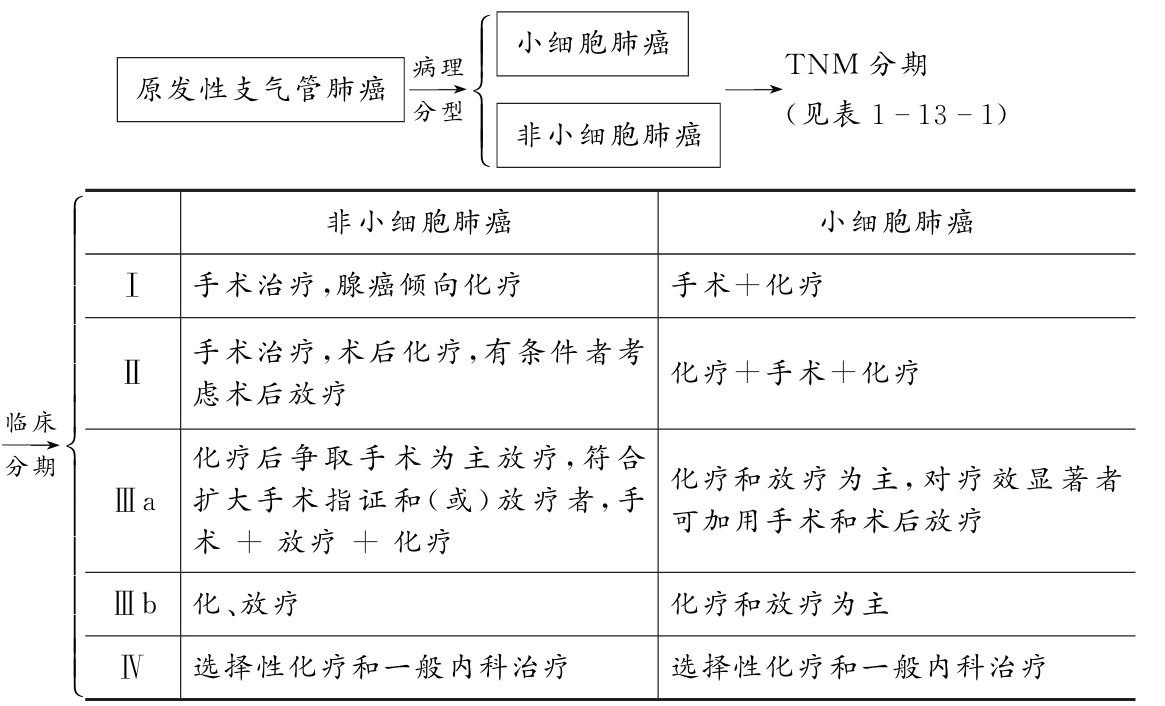
\includegraphics{./images/Image00028.jpg}
 \captionsetup{justification=centering}
 \caption{原发性支气管肺癌的治疗程序}
 \label{fig1-13-1}
  \end{figure} 

\begin{longtable}[]{p{15cm}}
  \caption{肺癌的TNM分期}
  \label{tab1-13-1}\\
\toprule
\endfirsthead
\caption[]{肺癌的TNM分期}\\
\toprule
\endhead
\bottomrule
\endfoot
 Tx: 原发肿瘤不能评估,或痰、支气管灌洗液找到癌细胞但影像学或支气管镜没有可见的肿瘤\tabularnewline
 To:没有原发肿瘤的证据\tabularnewline
 Tis:原位癌\tabularnewline
 T1:肿瘤最大径≤3cm,周围被肺或脏层胸膜所包绕,支气管镜下肿瘤侵犯没有超出叶支气管近端(即没有累及主支气管){a}\tabularnewline
  T1a 肿瘤最大径≤2cm\tabularnewline
  T2a 肿瘤最大径\textgreater{}2cm但≤3cm\tabularnewline
\vtop{\hbox{\strut  T2:肿瘤\textgreater{}3cm但≤7cm或者肿瘤具有以下任一特征{b}
:}\hbox{\strut    · 累及主支气管,但距隆突≥2cm}\hbox{\strut    ·
侵犯脏层胸膜}\hbox{\strut    ·
伴有扩展到肺门的肺不张或阻塞性肺炎,但未累及全肺}}\tabularnewline
  T2a 肿瘤最大径\textgreater{}3cm但≤5cm\tabularnewline
  T2b 肿瘤最大径\textgreater{}5cm但≤7cm\tabularnewline
 T3:肿瘤\textgreater{}7cm或肿瘤已直接侵犯下述结构之一者:胸壁(包括肺上沟癌)、膈肌、膈神经、纵隔胸膜、心包壁层;或肿瘤位于距隆突2cm以内的主支气管{a}
,但尚未累及隆突;或伴有累及全肺的肺不张或阻塞性肺炎或原发肿瘤同一叶内出现分散的单个或多个瘤结节\tabularnewline
 T4:任何大小的肿瘤已直接侵犯下述结构之一者:纵隔、心脏、大血管、气管、喉返神经、食管、椎体、隆突;同侧非原发肿瘤所在叶的其他肺叶出现分散的单个或多个瘤结节\tabularnewline
区域淋巴结(N)\tabularnewline
 Nx:区域淋巴结不能评价\tabularnewline
 No:没有区域淋巴结转移\tabularnewline
 N1: 转移至同侧支气管旁淋巴结和(或)同侧肺门淋巴结,和肺内淋巴结,包括直接侵犯\tabularnewline
 N2:转移至同侧纵隔和(或)隆突下淋巴结\tabularnewline
 N3:转移至对侧纵隔淋巴结、对侧肺门淋巴结、同侧或对侧斜角肌或锁骨上淋巴结\tabularnewline
远处转移(M)\tabularnewline
 Mx:远处转移不能评估\tabularnewline
 M0:无远处转移\tabularnewline
 M1:有远处转移\tabularnewline
  M1a 对侧肺叶出现分散的单个或多个瘤结节;胸膜结节或恶性胸腔(或心包)积液{c}\tabularnewline
  M1b 远处转移\tabularnewline
\end{longtable}


\begin{table}[htbp]
  \centering
  \caption{TNM与临床分期的关系}
  \label{tab1-13-2}
  \begin{tabular}{llll}
\toprule
0期 & Tis(原位癌) & Ⅲa期 & T1,N2,M0\tabularnewline
\midrule
Ⅰa期 & T1a,T1b,N0,M0 & & T2,N2,M0\tabularnewline
Ⅰb期 & T2a,N0,M0 & & T3,N1,M0\tabularnewline
Ⅱa期 & T1,T2b,N1,M0 & & T3,N2,M0\tabularnewline
Ⅱb期 & T2,N1,M0 & Ⅲb期 & T4,任何N,M0\tabularnewline
& T3,N0,M0 & & 任何T,N3,M0\tabularnewline
& & Ⅳ期 & 任何T,任何N,M1\tabularnewline
\bottomrule
  \end{tabular}

  注:隐性癌Tx,N0,M0不涉及分期
\end{table}


【治疗方案】 肺癌的治疗手段有多种,主要根据患者的机体状况,肿瘤的病理类型和临床分期采用相应的个体化的综合治疗措施,以期延长患者的生存时间、提高患者的生活质量。非小细胞肺癌(NSCLC)首选手术治疗,辅以化疗和放疗;小细胞癌(SCLC)多选用化疗加放疗加手术。

{(一)手术治疗}
 外科治疗是早期肺癌的最佳治疗方法。非小细胞肺癌Ⅰ期和Ⅱ期患者应行以治愈为目标的手术治疗。当病灶局限,未侵袭对侧及高位纵隔淋巴结时,可行肺叶、肺段、楔形、双肺叶及袖状切除术。当病变已累及同侧纵隔淋巴结或胸壁的Ⅲa患者(包括未侵及椎体和交感神经结的肺上沟瘤),仍可试行肿瘤切除加纵隔淋巴结清扫或胸壁重建。切除边缘无癌细胞者,其5年生存率为40\%以上。小细胞肺癌90\%以上就诊时已有胸内或远处转移,因此国内主张先化疗、后手术。

{(二)化学药物治疗}

1.
SCLC的化疗方案 小细胞肺癌对化疗非常敏感,推荐以化疗为主的综合治疗以延长患者的生存期。常用的联合方案是依托泊苷(VP-16)加顺铂(DDP)或卡铂(CBP),3周1次,共4\textasciitilde{}6个周期。也可在依托泊苷联合顺铂的基础上加用异环磷酰胺(IFO)。较大病灶经化疗后缩小,有助于手术及放疗。手术后或放疗后应继续化疗,一般术后2\textasciitilde{}3周可行化疗。目前临床一线化疗方案包括:

(1)EP方案:VP-16 120mg/(m{2}
·d),第1\textasciitilde{}3日静脉滴注;DDP 60mg/(m{2}
·d),静脉滴注第1日。每3周为1个周期。

(2)VP-CP方案:VP-16 120mg/(m{2}
·d),第1\textasciitilde{}3日静脉注射;CBP 100mg/(m{2}
·d),第1\textasciitilde{}3日静脉注射。每4周为1个周期。

(3)IP方案:CPT-11 60mg/(m{2} ·d),第1、8、15日静脉注射;DDP
80mg/(m{2} ·d),第1日静脉注射。每4周为1个周期。

二线化疗方案应首选临床新药试验;如肿瘤在3个月内复发且体质较好者,可考虑应用紫杉醇[100mg/(m{2}
·d)d1、8,每3\textasciitilde{}4周为1个周期]、多西紫杉醇、健择(吉西他滨,gemcitabine)及异环磷酰胺等;如肿瘤复发超过3个月以上,则可考虑应用拓扑替康[0.75mg/(m{2}
·d)d1\textasciitilde{}5;CBP
AUC=5d1;每3周为1个周期]、依立替康、CAV方案[环磷酰胺CTX1mg/(m{2}
·d)d1,阿霉素ADM 45\textasciitilde{}50mg/(m{2} ·d)d1,长春新碱VCR
1mg/(m{2}
·d)d1]、健择、紫杉醇、口服VP-16或诺维本等;肿瘤复发超过6个月以上者,仍可维持一线治疗方案。

2.
NSCLC的化疗方案 非小细胞肺癌对化疗的反应较差,目前主张对NSCLCⅠ、Ⅱ期患者手术后进行化疗,以防术后发生局部复发或远距离转移。Ⅲa患者应于术前、术后进行全身化疗,Ⅲb及Ⅳ期患者已不宜手术或放疗,化疗可延长生存期。一般化疗4个周期。目前临床常用的方案有:

(1)GP方案:吉西他滨 1000mg/m{2} ,第1、8日静脉滴注;DDP 80mg/m{2}
,第1日静脉滴注。每3周为1个周期。

(2)NP方案:NVB(长春瑞滨) 25mg/(m{2} ·d),第1、8日静脉滴注;DDP
75mg/(m{2} ·d),第1日静脉滴注(或总量分3日给予)。每4周为1个周期。

(3)TP方案:TXL(紫杉醇) 135mg/m{2} 第1日静脉滴注;DDP 60mg/(m{2}
·d),第3日静脉滴注。每3周为1个周期。

针对NSCLC一线化疗失败患者,单药多西他滨[75mg/(m{2}
·d),d1/3周]、培美曲赛[500mg/(m{2} ·d),d1/3周]或厄罗替尼(150mg
qd)、吉非替尼(250mg qd)常被用于二线治疗。

{(三)放射治疗}
 放射线对癌细胞有杀伤作用。肺癌对放疗的敏感性,以小细胞癌为最高,其次为鳞癌和腺癌,故照射剂量以小细胞癌最小,腺癌最大。一般40\textasciitilde{}70GY(4000\textasciitilde{}7000rad)为宜,分5\textasciitilde{}7周照射,常用的放射线有{60}
钴γ线,电子束β线和中子加速器等。应注意减少和防止白细胞减少、放射性肺炎、放射性肺纤维化和放射性食管炎等放疗反应。对全身情况太差,有严重心、肺、肝、肾功能不全者应列为禁忌。三维适形放疗技术(3DCRT)和调强放疗技术(IMRT)是目前最先进的放疗技术。

{(四)分子靶向治疗}
 目前临床常用的靶向药物为EGFR家族抑制剂和抗血管生成药。临床使用的EGFR家族抑制剂主要是吉非替尼(Gefitinib,易瑞沙)和厄罗替尼(Erlotinib,他昔瓦),用于EGFR突变阳性患者,FDA已批准厄罗替尼用于局部晚期或转移性的NSCLC。单克隆抗体西妥昔单抗(Cetuxmab,爱必妥Erbitux起始剂量400mg/m{2}
,维持剂量250mg/m{2}
)可联合化疗用于EGFR突变阳性的肺癌复发和转移的患者。常用抗血管生成药有贝伐单抗(Bevacizumab,阿瓦斯汀Avastin
15mg/kg,d1,每3周为1个周期)和血管内皮抑素(Endostatin)即恩度(Endostar
YH-16 7.5mg/m{2}
d1\textasciitilde{}14,每3周为1个周期),临床常联合化疗使用,抑制肿瘤血管生成,以起到抑制肿瘤生长的作用。贝伐单抗不应单药使用,国内尚未批准其用于NSCLC的一线治疗。许多其他靶向药物正在临床试验中。

{(五)肺癌介入性治疗}

1.
支气管动脉灌注化疗(BAI) 适用于失去手术指征,全身化疗无效的晚期癌患者,此方法不良反应小,可缓解症状,减轻患者痛苦。

2.
经纤支镜介导治疗 ①血卟啉染料激光治疗和YAG激光切除治疗:可解除肿瘤引起的气道阻塞和控制出血。②经纤支镜行腔内放疗:可缓解肿瘤引起的阻塞和咯血症状。③超声引导下的介入治疗,可直接将抗癌药物等注入肿瘤。

{(六)生物反应调节剂(biological response modifier,BRM)治疗}
 免疫生物治疗已成为肿瘤治疗的重要部分,如干扰素、白细胞介素2(IL-2)、肿瘤坏死因子(TNF)、集落刺激因子(CSF)等在小细胞肺癌的治疗中能增加机体对化疗、放疗的耐受性,提高疗效。

{(七)中医药治疗}
 目前临床广泛使用的还有一些抗肿瘤中药,其对肿瘤控制及改善患者生活质量均有一定疗效。参一胶囊由人参皂甙Rg3单一成分组成,人参皂甙Rg3是存在于传统中药人参中一种微量的四环三萜皂甙。该药尚可抑制肿瘤血管内皮细胞的增殖生长和新生血管的形成。临床使用可改善肿瘤患者的气虚症状,提高机体免疫功能。

【疗效观察与随访】

随访目的 ①及时发现治疗相关的各种并发症。②早期发现肿瘤复发转移,或第二原发癌(包括肺癌及其他肿瘤),有利于及时进行手术或放化疗。

1.
观察指标 观察内容包括:治疗前后患者的症状如咳嗽、咯血等变化情况;有无转移表现:脑、中枢神经系统(颅内压增高的征象)、肝、骨转移,有3\%\textasciitilde{}10\%的肺癌患者可发生,以小细胞肺癌居多;肺癌的肺外表现的变化,如肥大性肺性骨关节病,当肿瘤切除后,其症状可减轻或消失,肿瘤复发又可出现;实验室检查项目如血常规、血生化、肿瘤指标等;影像学如胸片、胸部CT、PET-CT等器械检查项目。

2.
临床治愈标准 症状、体征消失,术后愈合良好,肺功能正常,肿瘤标志物检测正常,胸部X线摄片或CT片肿块消失,一年内未复发。

3.
随访 建议对于Ⅰ\textasciitilde{}Ⅳ期的患者,在开始的2年里应每4\textasciitilde{}6个月进行1次常规病史回顾和体检,并行胸部增强CT扫描,而后每年1次非增强CT扫描及病史、体格检查。每次随访时应行吸烟状态评估,必要时建议戒烟。

【治疗经验与解析】

1.
治疗策略及注意事项 对于已经确诊支气管肺癌的患者,需要根据其病史、体格检查及相关必要检查结果明确临床分期,从而选择个体化治疗。有远处转移(Ⅳ期)的患者治疗策略取决于转移的部位,可通过纵隔镜检查、纤支镜,PET/CT扫描和脑MRI来帮助诊断。对选择性的、仅有单发转移灶的患者(Ⅳ期),尤其是单发脑转移患者,行转移灶切除可延长生存期。CT扫描发现肾上腺肿块的患者需行活检以排除良性肿瘤,如果发现肾上腺转移而肺部病变可切除,行肾上腺转移灶切除后可使部分患者获得长期生存。含铂的二联方案在毒性反应、使用方便性和费用上略有差别,应根据患者情况制定适宜的方案。目前推荐贝伐单抗联合紫杉醇加卡铂(PCB方案)用于治疗经选择的晚期NSCLC(非鳞癌)患者,但须满足以下标准:非鳞状细胞NSCLC,无咯血史。任何可能导致血小板减少并造成出血危险的方案与贝伐单抗联合使用时都需谨慎。对于4\textasciitilde{}6个周期化疗后肿瘤缓解或疾病稳定而没有发生进展的患者,可予维持治疗。非鳞状细胞癌患者在含铂两药联合方案一线化疗4\textasciitilde{}6个周期后可开始培美曲赛维持治疗。对于复发和远处转移患者,如为可切除的局部复发病灶,可再行手术切除或外放射治疗缩小肿瘤从而减轻症状。对于支气管腔内阻塞,特别是生命受到严重威胁的患者,减轻气道阻塞可以延长生存,改善生活质量,目前可采用近距离放疗(支气管腔内放疗)、激光治疗或支气管腔内支架置入。严重咯血的患者可选择激光治疗、栓塞治疗或手术切除出血部位等方式。有骨转移的患者应予双磷酸盐治疗。出现恶性胸腔积液或心包积液者予局部治疗处理,如携带式胸腔细管引流、胸膜固定术和心包开窗术,并应抽水检查,以排除其他需要积极治疗的病因,如充血性心力衰竭和感染。有30\%\textasciitilde{}45\%患者可能经历中至重度的癌性疼痛,应在准确疼痛评估的基础上予以合理的疼痛治疗,提高患者的生活质量。WHO及其他相关组织指出,联合使用非甾体类抗炎药、阿片类药物及辅助性药物可获得最佳止痛效果。

2.
化疗不良反应的处理要点 化疗过程中出现的不良反应应及时处理。常见的不良反应主要为胃肠道反应,如恶心、呕吐等,改变饮食习惯(少量多餐,禁食生冷、辛辣刺激性、油炸及含5-HT丰富的食物)和服用止吐药(如5-HT拮抗剂)能减轻这两种症状,对于治疗前恶心的患者,要进行心理劝导,分散其注意力。有时恶心、呕吐症状是继发于肿瘤进展导致的中空脏器梗阻、肠动力下降、代谢异常或中枢神经系统疾患,在可能情况下还需要纠正病因。出现骨髓抑制(主要表现为白细胞、血小板减少)的患者,针对白细胞减少(化疗期间出现时,需中止化疗),应及时给予升白治疗(粒细胞集落刺激因子G-CSF及粒-巨噬细胞集落刺激因子)。若出现Ⅳ度骨髓抑制应给予保护性隔离,预防性抗感染治疗,并密切监测血象变化。对于血小板减少的患者,应予升血小板治疗(当血小板低于20×10$^{9}$
/L时,建议输注浓缩血小板),并密切观察有无出血情况,及时处理。出现肝功能损害的患者及时给予保肝降酶处理,并监测肝功能情况。

\section{弥漫性间质性肺病}

弥漫性间质性肺病(diffuse interstitial lung
disease,DILD)或称间质性肺病(interstitial lung
disease,ILD)是指一组不同类型的非特异性的、侵犯肺泡壁及肺泡周围组织,X线显示两肺野弥漫性浸润的疾病的总称。本组疾病的病变主要发生于肺间质,但也常累及肺泡上皮细胞、肺泡毛细血管内皮细胞,以及细支气管等,故也称“弥漫性实质性肺病(diffuse
parenchymal lung
disease,DPLD)”。本病有近200种,大多数病因不明,发病机制不清,发病隐袭,呈慢性过程,偶可见急性发病,其临床、影像学和肺功能等具有某些共性,若无病理依据常难以确诊。2002年美国胸科学会(ATS)和欧洲呼吸学会(ERS)联合发表了间质性肺病分类共识报告,将DILD分为四大类:①已知病因的ILD:如职业性、药物性、结缔组织相关性ILD;②特发性间质性肺炎:包括特发性肺纤维化(IPF)、非特异性间质性肺炎(NSIP)、急性间质性肺炎(AIP)、隐源性机化性肺炎(COP)、呼吸性细支气管炎性间质性肺病(RB-ILD)、脱屑性间质性肺炎(DIP)、淋巴细胞性间质性肺炎等(LIP);③肉芽肿性疾病:结节病、肉芽肿性多血管炎、Churg-Strauss综合征等;④其他ILD:肺泡蛋白沉积症、淋巴管肌瘤病等。本章节重点对其中较为常见并有代表性的疾病加以概述。

\subsection{特发性肺纤维化}

特发性肺纤维化(idiopathic pulmonary
fibrosis,IPF)是指原因不明并以普通型间质性肺炎(UIP)病理改变为特征的一种慢性炎症性间质性肺疾病。IPF一般呈亚急性或慢性过程,主要表现为弥漫性肺泡炎、肺泡单位结构紊乱和肺纤维化。临床上多表现为进行性呼吸困难伴有刺激性干咳,双肺闻及捻发音,常伴有杵状指,胸部CT表现为双肺弥漫性网状影、后期形成蜂窝影,肺功能为限制性通气障碍,最后多死于呼吸衰竭和继发肺部感染。

【治疗程序】 图\ref{fig1-14-1}所示。

\begin{figure}[!htbp]
 \centering
 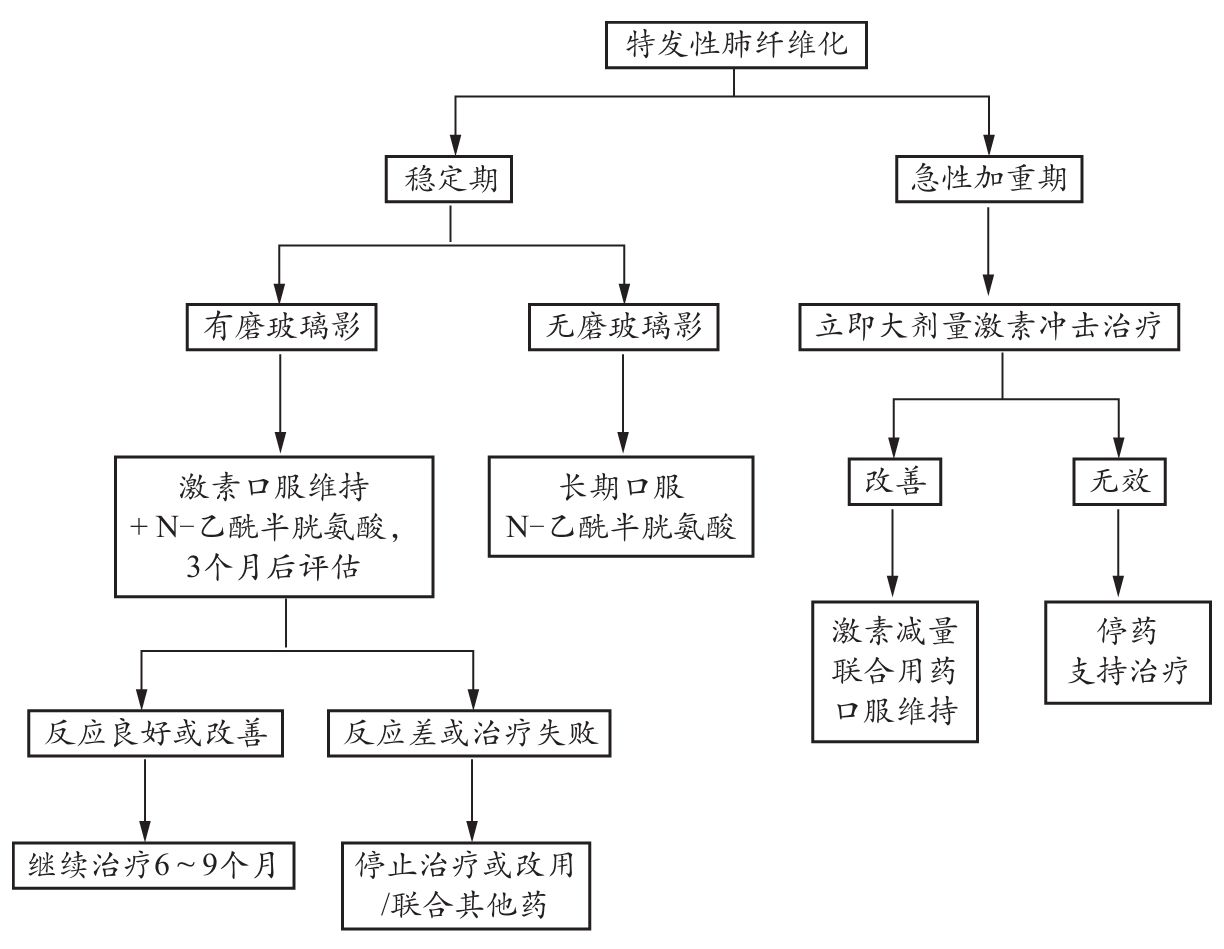
\includegraphics{./images/Image00029.jpg}
 \captionsetup{justification=centering}
 \caption{特发性肺纤维化的治疗程序}
 \label{fig1-14-1}
  \end{figure} 

【治疗方案】

{(一)一般治疗}
 IPF常有咳嗽,如果症状严重,应予止咳治疗。对已出现呼吸衰竭的患者应进行氧疗,长期氧疗能提高患者的生存质量。

{(二)药物治疗}

1.
稳定期的治疗 目前推荐糖皮质激素与细胞毒制剂(环磷酰胺或硫唑嘌呤)联合使用,但效果不肯定,多为专家意见,无循证医学证据。

(1)糖皮质激素:泼尼松初始第1\textasciitilde{}2个月剂量为0.5mg/(kg·d)(30\textasciitilde{}40mg/d),以后逐渐减量,到第6个月左右减至10mg/d,后6个月维持7.5\textasciitilde{}10mg/d。通常疗程在1年左右。但对仅表现为“蜂窝肺”而无磨玻璃改变者,皮质激素多不主张使用。对于年龄大于70岁,有激素禁忌证的患者,也尽量不使用激素治疗。

(2)细胞毒药物:首选硫唑嘌呤2\textasciitilde{}3mg/(kg·d),起始剂量为25\textasciitilde{}50mg/d,每7\textasciitilde{}14日增加25mg,常用量100mg/d,最大剂量150mg/d。也可选用环磷酰胺每日2mg/(kg·d)口服,起始剂量为25\textasciitilde{}50mg/d,每7\textasciitilde{}14日增加25mg,常用量100mg/d,最大剂量150mg/d;或环磷酰胺静脉滴注,每次400\textasciitilde{}600mg,每2周1次,总量8\textasciitilde{}12g。或环孢素A,每日5mg/kg,疗程3\textasciitilde{}6个月。

(3)N-乙酰半胱氨酸:具有抗氧化特性,可减缓肺功能下降,改善症状,可与糖皮质激素、细胞毒药物联合用药。600mg口服,每日3次,疗程6\textasciitilde{}12个月。

(4)吡非尼酮(Pirfenidone,PFD):能降低成纤维细胞增生,降低胞外基质产生,抑制转化生长因子β(TGF-β)介导的胶原合成,有可能减低IPF急性加重。每次200\textasciitilde{}600mg,每日3次,疗程6\textasciitilde{}9个月。

2.
急性加重期的治疗 目前多推荐大剂量糖皮质激素短期冲击治疗,迅速减量后再联合细胞毒药物等。一般剂量为甲泼尼龙每日500\textasciitilde{}1000mg,连续静脉滴注3日,很快减量至120mg/d,再3日,继续减量至40\textasciitilde{}80mg/d,连续3\textasciitilde{}5日,后改为泼尼松0.5mg/(kg·d)口服。必要时可加用免疫抑制剂如静脉滴注环磷酰胺及抗凝治疗,同时要加强预防感染、保护胃粘膜、补钙、氧疗等支持治疗。

{(三)肺移植}
 是目前唯一被证实能延长严重IPF的生存期及改善患者的生活质量的治疗方法,5年生存率约40\%。但仍面临诸多问题,如供体来源困难、费用昂贵、急慢性排斥反应的预防等。

【疗效观察与随访】

1. 观察指标

(1)症状、体征:观察咳嗽、呼吸困难的缓解情况。

(2)影像学:特别是HRCT对疗效评估有重要作用。

(3)肺功能检查:TCL、VC、DL{CO} 、PaCO{2} 、6分钟步行试验等指标。

2. 疗效标准

(1)痊愈:除肺移植外,尚无痊愈方法。

(2)好转:部分急性加重患者,通过激素冲击治疗后,可能会有好转,表现为呼吸困难减轻、呼吸衰竭纠正、HRCT上广泛的磨玻璃影吸收。

(3)缓解:大部分IPF患者自然病程即表现为缓慢逐步可预见的肺功能下降,但随着疾病的进展,呼吸困难程度会逐渐加重。

(4)无效:大多数IPF患者即使应用激素及免疫抑制剂治疗,病情依然恶化,呼吸困难加重,HRCT上蜂窝影逐渐增多、出现新的磨玻璃影等恶化指标均提示治疗无效。

3.
随访 一定要定期随访,注意糖皮质激素等药物长期使用过程中出现的不良反应的预防,注意病情变化,观察症状、体征等变化,避免合并症、并发症。

【治疗经验与解析】 治疗应根据个体化原则,治疗前应对患者的基本病情进行综合分析,评价患者的危险/疗效比,并在详细告知患者风险和益处后再开始治疗。对于年龄\textgreater{}70岁、极度肥胖、伴随严重蜂窝样改变以及HRCT缺乏磨玻璃影征象的患者,糖皮质激素疗效不明显,是否给予激素治疗一定要权衡利弊。

\subsection{隐源性机化性肺炎}

隐源性机化性肺炎(cryptogenic organizing
pneumonia,COP)是指没有明确的致病原(如感染、药物)或其他临床伴随疾病(如结缔组织病等)的情况下出现的机化性肺炎,病理特点是肺泡内、肺泡管、呼吸性细支气管及终末细支气管腔内有机化性肉芽组织,一般对糖皮质激素反应良好,过去称为闭塞性细支气管炎伴机化性肺炎(bronchiolitis
obliterans organizing pneumonia,BOOP)。

【治疗程序】 图\ref{fig1-14-2}所示。

\begin{figure}[!htbp]
 \centering
 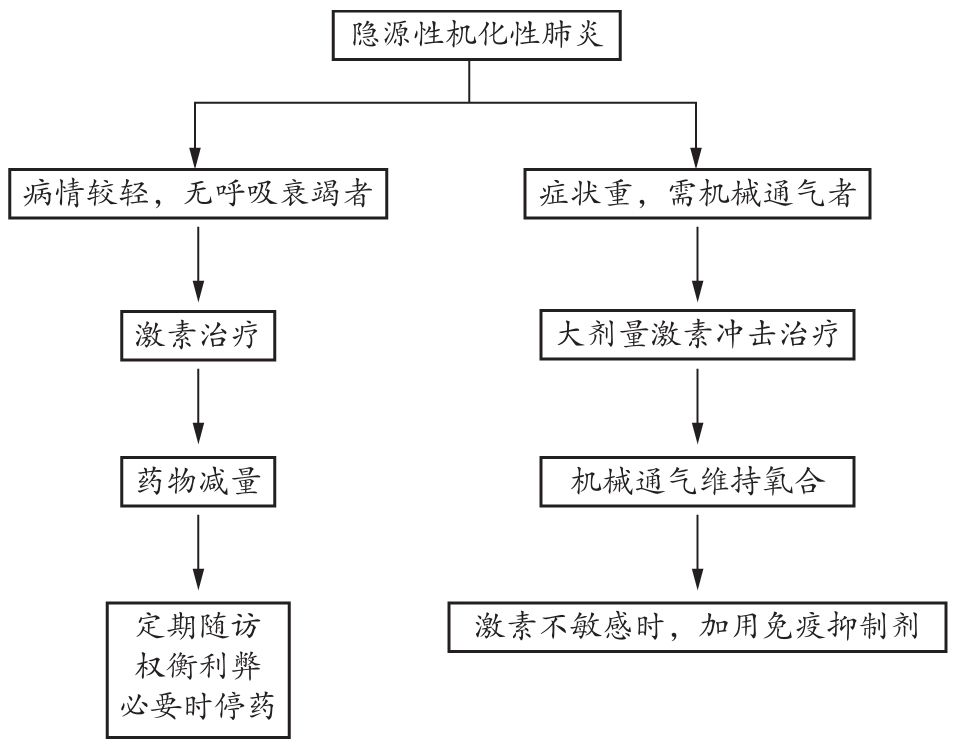
\includegraphics{./images/Image00030.jpg}
 \captionsetup{justification=centering}
 \caption{隐源性机化性肺炎的治疗程序}
 \label{fig1-14-2}
  \end{figure} 

【治疗方案】

{(一)一般治疗}

1.
治疗原则 COP对糖皮质激素治疗反应和预后均良好,故首选糖皮质激素治疗,少数COP患者可自行缓解。

2.
对症支持治疗 较重患者应卧床休息,呼吸困难和发绀显著者应给予氧疗。高热患者应给予退热、补液等支持治疗。

{(二)药物治疗}

1.
糖皮质激素 通常采用泼尼松0.75mg/(kg·d),约40mg/d,1\textasciitilde{}2个月,随后0.5mg/(kg·d),约30mg/d,治疗1个月,20mg/d治疗1\textasciitilde{}2个月,继续缓慢减量至维持量5\textasciitilde{}10mg/d。症状较重的病例可先静脉应用甲泼尼龙1\textasciitilde{}2mg/(kg·d)治疗3\textasciitilde{}5日。急性进展型可用甲泼尼龙0.5\textasciitilde{}1.0g静滴,冲击治疗3\textasciitilde{}5日,继用泼尼松口服。

2.
免疫抑制剂 效果较差,较少应用。病情严重、对糖皮质激素长期或短期疗效不佳的患者,特别是合并结缔组织疾病者,可考虑使用环磷酰胺(CTX);在急性或严重的病例中,也可短时间用环磷酰胺(400mg/次,2次/周)治疗。

【疗效观察与随访】

1. 观察指标

(1)症状、体征:观察咳嗽、呼吸困难、发热的缓解情况。

(2)影像学:特别是HRCT对疗效评估有重要作用。

(3)合并症:特别是注意是否有合并肺结核、肺部真菌感染等。

2. 疗效标准

(1)痊愈:预后良好,大部分患者在经过激素治疗后,临床症状及胸部影像学表现能迅速改善,如果治疗后肺功能恢复正常、HRCT上原有病灶完全吸收可以基本判断痊愈。

(2)好转:呼吸困难减轻、低氧血症纠正、HRCT上各种表现形式的病灶较治疗前均有吸收,可以判为好转。

(3)缓解:部分患者激素治疗后可以表现为临床症状缓解,但胸部HRCT上的病灶吸收不明显,此类患者治疗时间往往较长。

(4)无效:极少数COP患者对激素不敏感,呼吸困难不能缓解,影像学没有吸收,此时要考虑诊断是否正确,或是联合免疫抑制剂。

3.
随访 一定要定期随访,注意激素长期使用过程中出现的不良反应的预防,注意病情变化,观察症状、体征等变化,避免合并症、并发症。

【治疗经验与解析】 大多数患者会在治疗1周后出现明显的临床症状的改善,部分患者临床表现可在48小时内好转,多数经糖皮质激素治疗能完全缓解,但肺部影像学恢复较慢,疗程通常需1年。应注意在激素减量(通常\textless{}20mg/d)或停药1\textasciitilde{}3个月内,有相当数量的患者复发,一般情况下,复发患者仍可再次使用激素治疗。严重病例接受激素治疗数日内症状无改善,或激素减量后复发的患者可以考虑使用免疫抑制剂。

\subsection{结节病}

结节病(sarcoidosis)是一种原因未明、免疫介导的以非干酪性上皮样肉芽肿为病理特征的多系统性疾病。临床表现通常以侵犯肺、双侧肺门淋巴结为主,也可累及皮肤、眼、心脏、肝脏、脾脏、唾液腺、肌肉骨骼、肾脏及中枢神经系统,几乎全身每个器官均可受累。临床表现无特异性,部分患者无症状,大多数患者有自限性,约60\%患者可自然缓解,预后良好。

【治疗程序】 图\ref{fig1-14-3}所示。

\begin{figure}[!htbp]
 \centering
 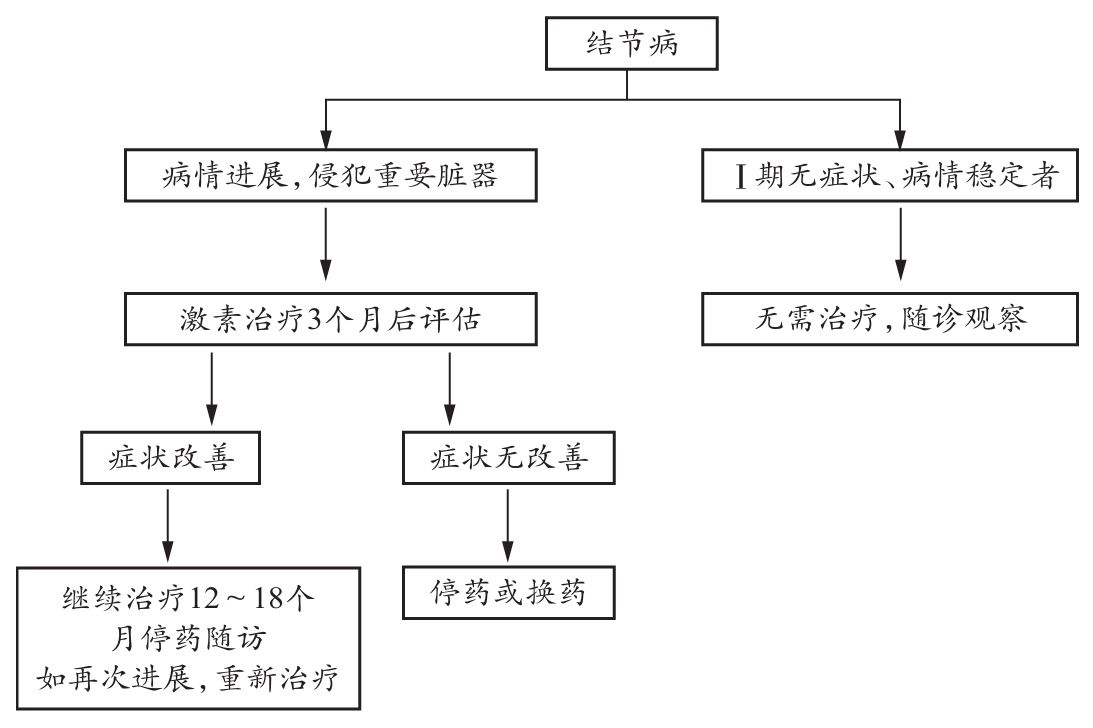
\includegraphics{./images/Image00031.jpg}
 \captionsetup{justification=centering}
 \caption{结节病的治疗程序}
 \label{fig1-14-3}
  \end{figure} 

【治疗方案】

{(一)治疗原则}

1.
病情稳定,无症状的患者特别是Ⅰ期患者多数可自行缓解,不需治疗,每3\textasciitilde{}6个月随访1次。

2.
凡症状明显的Ⅱ、Ⅲ期患者,特别是有重要器官功能损害(如肺功能损害),及胸外结节病累及重要脏器如眼结节病、神经系统结节病、心脏结节病、恶性高钙血症等均需积极治疗。

{(二)药物治疗}

1. 糖皮质激素是首选治疗药物

(1)口服:初始治疗,泼尼松30\textasciitilde{}40mg/d,口服4\textasciitilde{}8周内可有明显症状改善,泼尼松剂量应逐步减少到每日5\textasciitilde{}10mg,或隔日1次服用。治疗后3个月无反应的患者通常不会对更长的疗程有反应。总疗程至少持续12个月或18个月。

(2)吸入:目前无循证医学证据表明吸入激素对结节病治疗有效,但对咳嗽明显或气道高反应性患者可以试用吸入激素缓解症状。

2. 细胞毒药物及免疫调节剂

(1)甲氨蝶呤:对皮肤损害和肺泡炎有一定的疗效,主要用于慢性、严重、难治性的结节病,常用剂量为每周1次口服10\textasciitilde{}15mg,疗程3\textasciitilde{}6个月。

(2)羟氯喹:对皮肤和粘膜结节病效果较好,对肺结节病亦有一定疗效,200\textasciitilde{}400mg/d,1次口服,连用6个月,注意眼部毒性。

(3)硫唑嘌呤:对激素无效者可以试用,每日50\textasciitilde{}200mg,分3\textasciitilde{}4次口服,疗程3个月。

(4)环孢素A:有报道本品5\textasciitilde{}7mg/(kg·d)联合应用泼尼松20mg/d治疗结节病,但疗效尚不确切。

3.
TNF-α活性药物 个案报道英夫利昔单抗治疗复杂的或复发的结节病有效,沙利度胺在特定的皮肤损害治疗中有效,但对肺结节病疗效报道较少。

【疗效观察与随访】

1. 观察指标

(1)症状、体征:观察咳嗽、呼吸困难的缓解情况,是否有新发眼部、皮肤、粘膜损害。

(2)影像学:特别是HRCT对疗效评估有重要作用。

(3)肺外系统检查:如肝肾功能、心电图、血钙、血管紧张素转化酶等指标。

2. 疗效标准

(1)痊愈:肺部症状消失、肺外表现消失、胸部HRCT上病灶完全吸收可以判定为痊愈,结节病有一定的自愈倾向。

(2)好转:肺部症状减轻、肺外表现减轻、HRCT上各种表现形式的病灶较治疗前均有吸收,可以判为好转。

(3)缓解:部分患者激素治疗后可以表现为临床症状缓解,但胸部HRCT上的病灶吸收不明显,此类患者治疗时间往往较长。

(4)无效:极少数结节病患者对激素不敏感,肺部或肺外症状不能缓解,影像学没有吸收,此时要考虑诊断是否正确,或是联合免疫抑制剂。

3.
随访 一定要定期随访,注意激素长期使用过程中出现的不良反应的预防,注意病情观察,观察症状、体征等变化,避免合并症、并发症。

【治疗经验与解析】 应用糖皮质激素治疗者在减量过程中或停药后复发率可达20\%\textasciitilde{}70\%,复发者对糖皮质激素治疗通常仍然有效,但需给予较大剂量或更长时间的维持治疗以防止再次复发。大部分患者泼尼松剂量需要20mg以上,可同时加用免疫抑制剂,如甲氨蝶呤、硫唑嘌呤等。对频繁复发者可能需要长期低剂量糖皮质激素维持治疗。

\subsection{过敏性肺炎}

过敏性肺炎(hypersensitivity
pneumonitis,HP),亦称外源性过敏性肺泡炎(extrinsic allergic
alveolitis,EEA),是一组由于反复吸入外界某些具有抗原性的有机粉尘所引起的肺部炎症病变。组织病理学以肺间质单核细胞性炎性渗出、细胞性细支气管炎和散在分布的非干酪样坏死性肉芽肿为特征性改变。各种病因所致EEA的临床表现相同,通常根据其临床特征分为急性、亚急性和慢性型。

【治疗程序】 图\ref{fig1-14-4}所示。

\begin{figure}[!htbp]
 \centering
 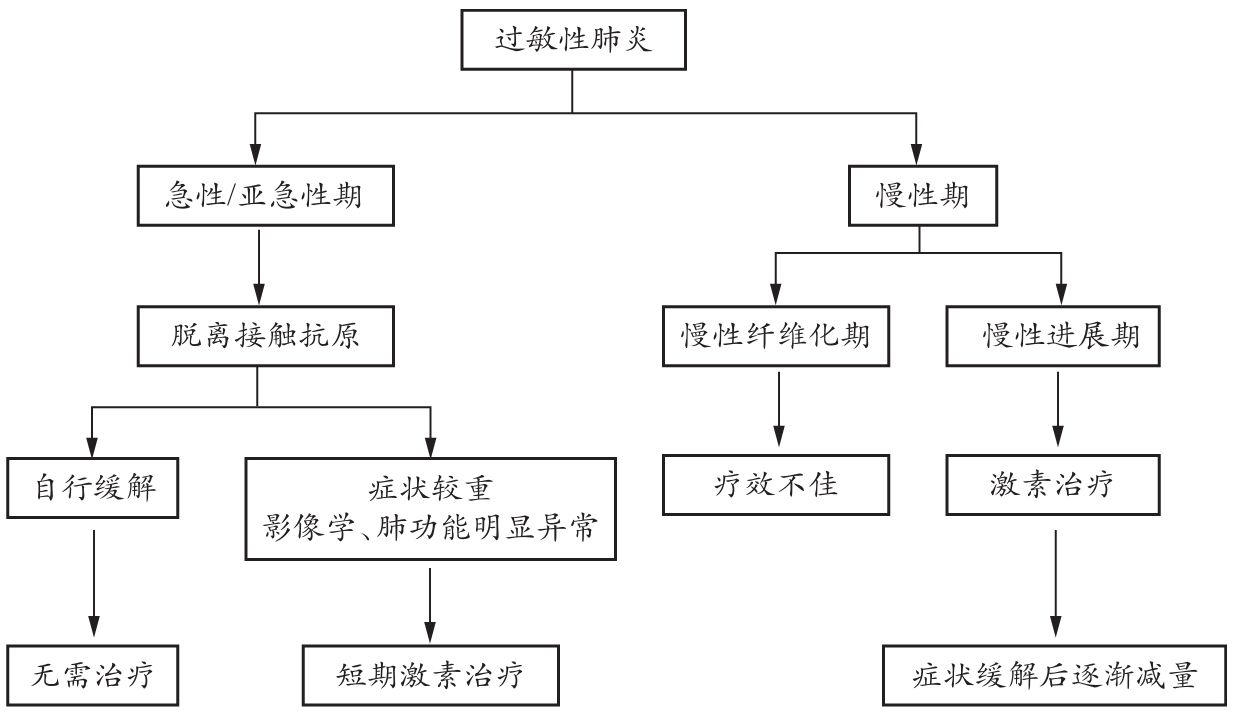
\includegraphics{./images/Image00032.jpg}
 \captionsetup{justification=centering}
 \caption{过敏性肺炎的治疗程序}
 \label{fig1-14-4}
  \end{figure} 

【治疗方案】

{(一)治疗原则}

1. 脱离或避免抗原接触 是最根本的防治措施。

2.
对症支持治疗 单纯的轻微呼吸道症状在避免抗原接触后可以自发缓解,不必特殊治疗。较重患者应卧床休息,呼吸困难和发绀显著者应给予氧疗。

{(二)药物治疗}
 糖皮质激素:急性期或亚急性期特别是伴有明显肺部渗出和低氧血症者,应该考虑使用糖皮质激素治疗,一般使用泼尼松30\textasciitilde{}60mg/日,分次口服,1\textasciitilde{}2周后根据临床、影像学和肺功能改善状况减量。急性期疗程4\textasciitilde{}6周,亚急性期疗程3\textasciitilde{}6个月。慢性期对尚存的肺泡炎有一定作用,疗程6个月以上,但对已形成的肺纤维化则无明显效果。

【疗效观察与随访】

1. 观察指标

(1)症状、体征:观察咳嗽、呼吸困难、胸闷的缓解情况,肺部啰音变化,乏力、发热等全身症状有无好转。

(2)影像学:特别是HRCT对疗效评估有重要作用。

2. 疗效标准

(1)痊愈:肺部症状消失、胸部HRCT上病灶完全吸收可以判定为痊愈,多数过敏性肺炎的疗效均佳。

(2)好转:肺部症状减轻、HRCT上各种表现形式的病灶较治疗前均有吸收,可以判为好转。

(3)缓解:部分患者激素治疗后可以表现为临床症状缓解,但胸部HRCT上的病灶吸收不明显,此类患者治疗时间往往较长。

(4)无效:极少数过敏性肺炎病患者对激素不敏感,肺部症状不能缓解,影像学没有吸收,可能与持续暴露有关。

3.
随访 2\textasciitilde{}3个月定期随访,注意激素长期使用过程中出现的副作用的预防,注意病情观察,观察症状、体征等变化,避免合并症、并发症。

【治疗经验与解析】 完全避免接触致病有机抗原是最根本的防治措施。短期糖皮质激素对急性和亚急性期治疗有较好疗效。

\subsection{弥漫性泛细支气管炎}

弥漫性泛细支气管炎(diffuse
panbronchiolitis,DPB)是以呼吸性细支气管等终末气道为主要病变部位的弥漫性炎症性疾病,为一种具有特异性的、独立的小气道疾病。由于炎症病变弥漫性的分布并累及呼吸性细支气管壁的全层,故称为弥漫性泛细支气管炎。除细支气管病变外,鼻窦也是DPB的常见病变部位。

【治疗程序】

\begin{figure}[!htbp]
 \centering
 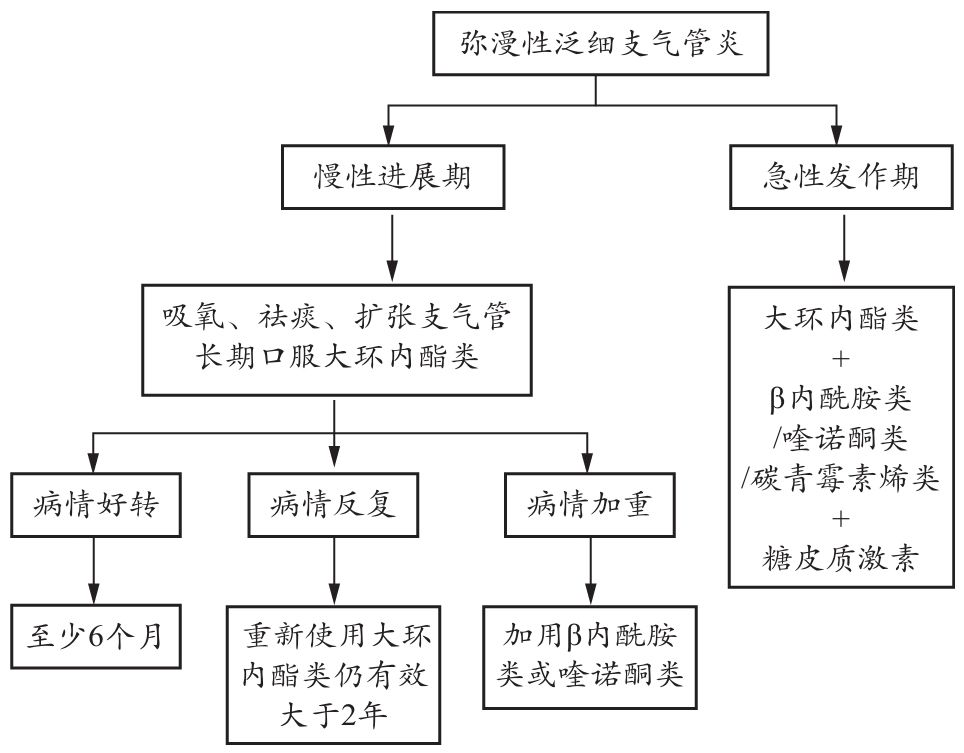
\includegraphics{./images/Image00033.jpg}
 \captionsetup{justification=centering}
 \caption{弥漫性泛细支气管炎的治疗程序}
 \label{fig1-14-5}
  \end{figure} 

【治疗方案】

{(一)治疗原则}
 目前主要以大环内酯类抗生素为首选药物的综合治疗,因大环内酯类药物具有抗炎和免疫调节作用,并可抑制铜绿假单胞菌生物被膜的形成,因而可改善本病的症状并明显提高生存率,而与其抗感染作用关系较小。

{(二)药物治疗}

1.
无论痰培养结果如何,均首选大环内酯类,一般初期病例口服红霉素400\textasciitilde{}600mg/日,连续6个月以上,病情进展的病例可使用2年以上。停药后复发的病例,再次使用红霉素仍然有效。其他大环内酯类抗生素(罗红霉素、克拉霉素、阿奇霉素等)与红霉素疗效相同,但十六元环大环内酯类无效。对于红霉素治疗1个月无效者,可换为克拉霉素或罗红霉素治疗。

2.
如出现感染征象(发热、脓痰、痰量增多、血象升高、CRP升高、ESR增快等),应早期留取痰标本送细菌培养及药敏试验,并根据药敏试验选择敏感抗菌药物。早期可经验性给予第3代或4代头孢菌素、β内酰胺类/β内酰胺酶抑制剂、喹诺酮类、氨基糖苷类等,最好能选择具有抗铜绿假单胞杆菌活性的抗菌药物。使用其他抗生素时,不停用大环内酯类。

3.
对糖皮质激素的应用尚有争议,一般认为适用于有气道痉挛的患者,轻者可雾化吸入,严重病例可静脉使用。

4. 对症治疗 祛痰药、支气管扩张药、鼻窦炎的治疗、免疫增强等。

【疗效观察与随访】

1. 观察指标

(1)症状、体征:开始治疗后,应立即观察患者咳嗽、咳痰的情况,并注意痰量痰色变化,观察肺部啰音变化,以此判断初期疗效。

(2)影像学:胸片、特别是HRCT对疗效评估有重要作用。

(3)实验室检查:后期随访应关注肺功能、动脉血气指标等。

2. 疗效标准

(1)痊愈:本病尚无痊愈方法。

(2)好转:肺部症状减轻、HRCT上各种表现形式的病灶较治疗前均有吸收,可以判为好转。

(3)缓解:部分患者治疗后可以表现为临床症状缓解,但胸部HRCT上的病灶吸收不明显,此类患者今后反复发作可能性较大。

(4)无效:如有多重耐药菌或难治性病原体感染,则治疗十分困难,表现为感染症状加重、甚至出现呼吸衰竭等,影像学较前进展,多提示预后不良。

3.
随访 初期治疗2周至1个月后应开始随访,之后每3个月随访1次,疗程1\textasciitilde{}2年。

{(四)预后}
 自1985年红霉素在治疗DPB上的应用开始,DPB的死亡率已从10\%下降至2\%左右,总体预后良好。

【治疗经验与解析】 如红霉素等大环内酯类抗生素用药3个月无效,则应怀疑快速进展的DPB或将其他疾病误诊为DPB,应仔细追查原因,及时调整治疗方案。

\subsection{肺泡蛋白沉积症}

肺泡蛋白沉积症(pulmonary alveolar
proteinosis,PAP)是一种以肺泡内大量沉积磷脂蛋白样物质为特点的肺部弥漫性疾病。目前诊断PAP的基本手段为临床症状(呼吸困难为主)、胸部HRCT(双肺弥漫性地图样分布实变影、铺路石样改变磨玻璃影)、支气管肺泡灌洗液(特征性的“牛奶”状液体,光镜下可见PAS阳性脂蛋白物质)以及经支气管经肺活检(肺泡腔内充满PAS阳性嗜伊红物质)。

【治疗程序】 图\ref{fig1-14-6}所示。

\begin{figure}[!htbp]
 \centering
 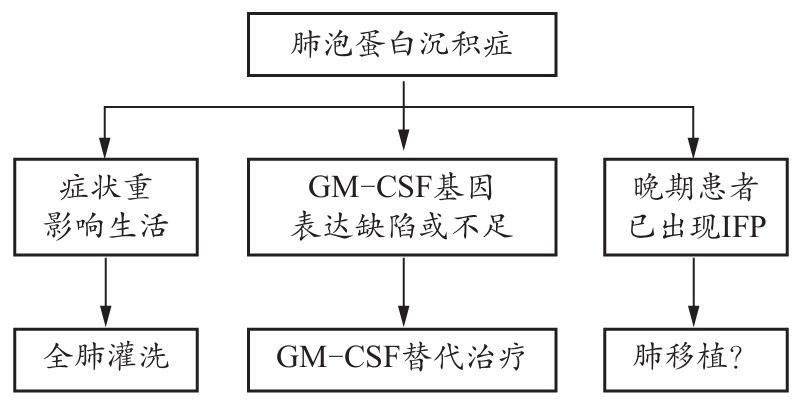
\includegraphics{./images/Image00034.jpg}
 \captionsetup{justification=centering}
 \caption{肺泡蛋白沉积症的治疗程序}
 \label{fig1-14-6}
  \end{figure} 

【治疗方案】

1.
全肺灌洗 是目前治疗PAP最有效的方法,适应证为明显的呼吸困难症状,活动后低氧血症,肺内分流\textgreater{}10\%。

2.
GM-CSF替代治疗 对确定由粒细胞-巨噬细胞集落刺激因子(GM-CSF)基因表达缺陷或不足引起的PAP患者,可给予GM-CSF替代治疗。一般给予皮下注射重组人的GM-CSF
5\textasciitilde{}9μg/(kg·d),疗程3个月左右,近半数患者有较好效果。亦有文献报道采用雾化吸入GM-CSF治疗有效。

3.
肺移植 对于晚期已发生严重肺纤维化的患者,有报道可进行肺移植,但移植肺仍有可能再发生PAP。

【疗效观察与随访】

1. 观察指标

(1)症状、体征:观察咳嗽、呼吸困难、肺部爆裂音等的变化情况。

(2)影像学:特别是HRCT对疗效评估有重要作用。

(3)支气管镜检查:肺泡灌洗液颜色、镜下改变等的变化。

2. 疗效标准

(1)痊愈:除肺移植外,本病尚无痊愈方法。

(2)好转:肺部症状减轻、HRCT上各种表现形式的病灶较治疗前均有吸收,可以判为好转。

(3)缓解:部分患者治疗后可以表现为临床症状缓解,但胸部HRCT上的病灶吸收不明显,此类患者今后反复发作可能性较大。

(4)无效:极少数患者虽经全肺灌洗术,但症状无法缓解,或出现灌洗术后症状加重,则治疗十分困难,表现为呼吸困难加重、甚至出现呼吸衰竭等,影像学较前进展,多提示预后不良。

3.
随访 要定期随访,注意病情变化,观察症状、体征等变化,避免合并症、并发症。

【治疗经验与解析】 全肺灌洗要点:通常分2次完成左、右两肺的灌洗过程,间隔时间一般3\textasciitilde{}7日。首先选择病变严重侧肺,全麻下经Carlens双腔气管内导管进行全肺灌洗,每次灌注预热生理盐水500\textasciitilde{}1000ml,反复灌洗,直至洗出液完全清亮为止,一侧肺通常需要10\textasciitilde{}20L生理盐水。病变较局限者可经支气管镜支气管肺泡灌洗,但效果较差。

\subsection{肺朗格汉斯细胞组织细胞增多症}

肺朗格汉斯细胞组织细胞增多症(pulmonary Langerhans' cell
histiocytosis,PLCH),也称组织细胞增多症X,是一种病理以肺部朗格汉斯细胞增生浸润、胸部X线显示双肺多发的细支气管旁间质结节和囊腔为特征的慢性肺疾病,是组织细胞增多症的一种成人类型。本病为罕见病,多发生于成年男性吸烟者,确诊需典型的组织病理学证据。

【治疗程序】 图\ref{fig1-14-7}所示。

\begin{figure}[!htbp]
 \centering
 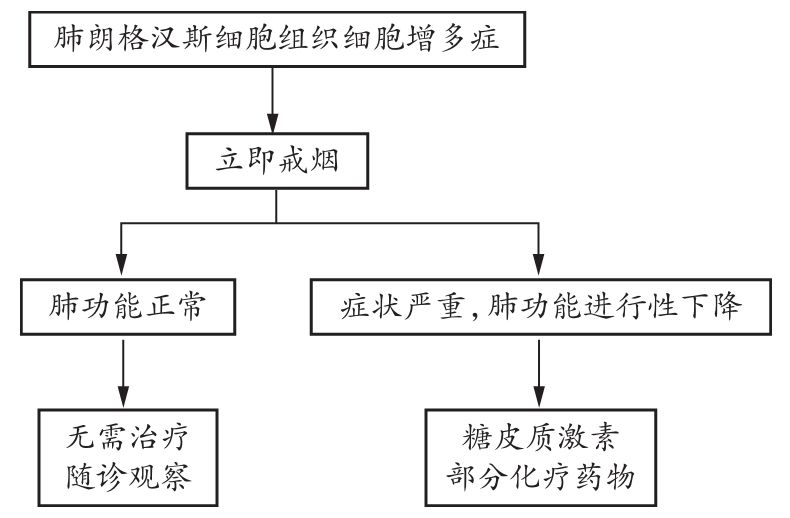
\includegraphics{./images/Image00035.jpg}
 \captionsetup{justification=centering}
 \caption{肺朗格汉斯细胞组织细胞增多症的治疗程序}
 \label{fig1-14-7}
  \end{figure} 

【治疗方案】

{(一)一般治疗}

1.
治疗原则 吸烟与疾病的进展与复发关系密切,患者必须立即戒烟。症状严重、肺功能进行性下降的患者可以给予糖皮质激素及化疗。

2.
对症支持治疗 较重患者应卧床休息,呼吸困难和发绀显著者应给予氧疗。合并气胸者,外科胸膜粘连术是最佳选择,但不宜用于打算肺移植的患者。

{(二)药物治疗}

1.
糖皮质激素 泼尼松初始剂量为0.5\textasciitilde{}1mg/(kg·d)(30\textasciitilde{}60mg/d),逐渐减量,连续使用6\textasciitilde{}12个月。

2.
化疗药物 如长春新碱、甲氨蝶呤、环磷酰胺、依托泊苷(VP-16)等可以用于对激素没有反应的多器官受累的患者。依托泊苷用法为150\textasciitilde{}200mg/(m{2}
·d)静脉滴注,或300\textasciitilde{}400mg/(m{2}
·d)口服3日,每疗程间隔3\textasciitilde{}4周,共2\textasciitilde{}6个疗程。

{(三)肺移植}
 PLCH伴有呼吸衰竭或肺动脉高压是肺移植的适应证,文献报道1年、2年和5年生存率分别为63.6\%、57.2\%和53.7\%,移植肺脏中20\%再发PLCH。

【疗效观察与随访】

1. 观察指标

(1)症状、体征:观察咳嗽、呼吸困难、营养状态等的变化情况。

(2)影像学:特别是HRCT对疗效评估有重要作用。

(3)肺功能检查:TCL、VC、DL{CO} 、PaCO{2} 、6分钟步行试验等指标。

(4)合并症:特别应注意是否有合并气胸、肺部感染等。

2. 疗效标准

(1)痊愈:戒烟后,本病有一定自愈倾向。

(2)好转和缓解:75\%患者在戒烟6\textasciitilde{}24个月病情缓解,肺部症状缓解,HRCT上各种表现形式的病灶较治疗前均有吸收。

(3)无效:经治疗后咳嗽、呼吸困难无改善,胸部影像学进一步进展,肺功能下降均提示治疗无效。

3.
随访 一定要定期随访,注意激素长期使用过程中出现的不良反应的预防,注意病情变化,观察症状、体征等变化,避免合并症、并发症。

【治疗经验与解析】 PLCH的临床病程差异很大,约70\%的患者病情可以自然缓解或经激素治疗而稳定或改善。

\subsection{硅沉着病}

硅沉着病又称矽肺(silicosis),是最常见的职业相关性间质性肺病类型,是由于反复吸入微小的游离二氧化硅晶体颗粒导致的以肺部弥漫性纤维化为主的疾病。石英是最常见的游离二氧化硅存在形式,可广泛存在于采矿、建筑、机械及材料制造等职业环境中。

【治疗程序】 略。

【治疗方案】

{(一)治疗原则}

1. 脱离或避免再接触游离二氧化硅。

2. 呼吸困难者应予氧疗,继发感染者予抗感染治疗。

{(二)药物治疗}

1.
典型矽肺 为提高药物疗效和降低不良反应,可采用药物联用,目前比较公认的联合用药方案有:

(1)粉防己碱(汉防己甲素)100mg每日2次口服+羟基磷酸哌喹0.5g每周1次口服,3个月为1个疗程,休息1\textasciitilde{}2个月后继续下一个疗程,共6个疗程。

(2)汉防己甲素100mg每日口服2次+克矽平(1\%克矽平144ml)每年1次支气管镜下滴注,共2次。

(3)柠檬酸铝20mg每周1次肌内注射+羟基磷酸哌喹0.25g每周2次口服,3个月为1个疗程,休息1\textasciitilde{}2个月后继续下1个疗程,共6个疗程。

2.
急性矽肺 也称硅肺蛋白沉积症(silicoproteinosis),有报道用糖皮质激素治疗取得一定疗效,但尚缺乏大样本报道证实。

{(三)全肺灌洗治疗}
 对全肺灌洗治疗矽肺目前尚有争议,有学者认为可改善部分症状,但对已形成的肺纤维化病变无治疗作用。对于急性矽肺,灌洗可以直接去除肺泡腔内大量的脂蛋白和粉尘,可以有效改善氧合,但不能清除肺间质内沉积的二氧化硅,所以患者往往需反复全肺灌洗治疗。全肺灌洗治疗矽肺可用生理盐水,也可以用0.04\%克矽平生理盐水。

【疗效观察与随访】

1. 观察指标

(1)症状、体征:观察咳嗽、呼吸困难、胸闷的缓解情况,肺部啰音变化,乏力、食欲缺乏等全身症状有无好转。

(2)影像学:胸片、特别是HRCT对疗效评估有重要作用。

(3)合并症:特别应注意是否有合并肺结核、肺部感染、气胸等。

2. 疗效标准

(1)痊愈:除肺移植外,本病尚无痊愈方法。

(2)好转和缓解:咳嗽、呼吸困难、胸闷均缓解,氧合状况好转,HRCT上病灶较前吸收。

(3)无效:经治疗后咳嗽、呼吸困难无改善,胸部影像学进一步进展,肺功能下降均提示治疗无效。

3.
随访 3\textasciitilde{}6个月内定期行胸部X线摄片、肺功能检查及临床症状观察。

【治疗经验与解析】 矽肺关键在于预防,降低工作环境粉尘,进行生产技术改革,从根本上消除粉尘产生,加强医学预防措施,做好健康检查,定期随访。

\subsection{药物性肺部疾病}

药物性肺部疾病(drug-induced lung
diseases,DILD)是指一大类由药物引起的肺病。药物对于肺的不良反应多种多样,可以是暂时、可逆的,停药后即可恢复,亦可以是永久性损害,停药已不能恢复;起病方式、病情程度均多样。药源性肺病没有明确的诊断标准,详细询问患者的用药史相当重要。

药物性肺部疾病的表现形式多种多样,常见的形式有:①肺间质纤维化(博来霉素、甲氨蝶呤、硫唑嘌呤、胺碘酮等);②过敏性肺炎(卡马西平、呋喃妥因、对氨基水杨酸等);③机化性肺炎(博莱霉素、乙胺碘肤酮、金制剂等);④支气管痉挛(非类固醇类抗炎药、β受体阻滞剂等);⑤非心源性肺水肿(海洛因、阿霉素、对乙酰水杨酸等);⑥呼吸衰竭(三环类抗抑郁剂、氨基糖苷类抗生素);⑦肺血管炎(青霉素、四环素、阿奇霉素等);⑧胸膜病变(白介素2、溴隐亭、丙卡巴肼等);⑨系统性红斑狼疮类症候群(青霉胺、肼屈嗪、普鲁卡因胺、异烟肼、乙内酰脲类)等。

【治疗程序】 图\ref{fig1-14-8}所示。

\begin{figure}[!htbp]
 \centering
 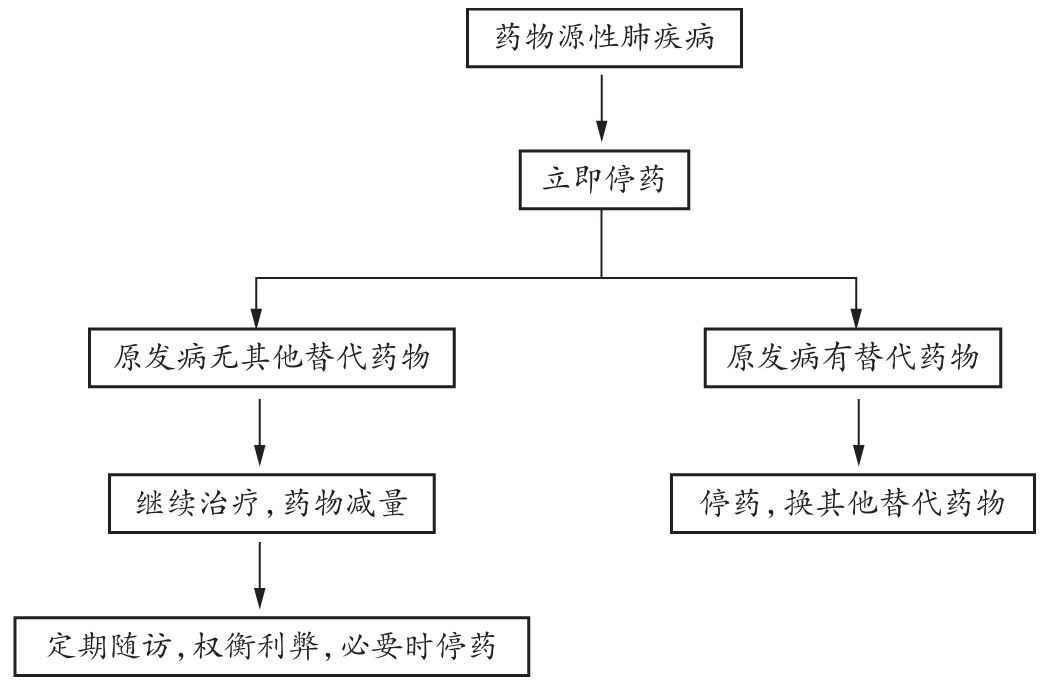
\includegraphics{./images/Image00036.jpg}
 \captionsetup{justification=centering}
 \caption{药物性肺疾病的治疗程序}
 \label{fig1-14-8}
  \end{figure} 

【治疗方案】

{(一)治疗原则}  以停药及抗过敏治疗为主,并给予对症处理。

{(二)药物治疗}

1.
糖皮质激素,一般30\textasciitilde{}60mg/日,根据病情逐渐减量,对过敏性肺炎、肺血管炎表现的患者疗效最佳。

2.
如有药物过敏,可给予抗组胺药物治疗;如为氨基糖苷类抗生素引起的呼吸衰竭,可给予注射新斯的明对抗治疗。

【疗效观察与随访】

1. 观察指标

(1)症状、体征:观察咳嗽、发热、呼吸困难、乏力、肌痛、关节痛等表现的缓解情况,亦要注意原发病的症状及体征变化。

(2)实验室检查:注意监测肝肾功能、肺功能、X线胸片等。

2. 疗效标准

(1)痊愈:大部分患者在停药及抗过敏治疗后均可以痊愈,表现为临床症状完全消失、肺部影像学病灶完全吸收。

(2)好转:肺部症状减轻、HRCT上各种表现形式的病灶较治疗前均有吸收,可以判为好转。

(3)缓解:部分患者治疗后可以表现为临床症状缓解,但胸部HRCT上的病灶吸收不明显,此类患者治疗时间可能需延长。

(4)无效:极少数患者经治疗后咳嗽、呼吸困难无改善,胸部影像学进一步进展,肺功能下降均提示治疗无效。

3.
随访 停止原发病的治疗后应密切观察原发病的变化,如需要继续治疗者,在明确引起损伤的具体药物后,调整治疗方案,密切观察。

{(四)预后}
 以过敏性损伤为主要表现者一般停药后可自行缓解,但已造成肺纤维化者预后差。

【治疗经验与解析】 药物性肺部疾病关键在于预防,临床医生应熟悉所用药物的药理作用及不良反应。合理用药,严格掌握适应证、禁忌证,尽量简化用药。

\section{胸膜疾病}

\subsection{胸腔积液}

胸膜腔是位于肺和胸壁之间的一个潜在的腔隙。在正常情况下脏层胸膜和壁层胸膜表面上有一层很薄的液体,在呼吸运动时起润滑作用。胸膜腔和其中的液体并非处于静止状态,在每一次呼吸周期中胸膜腔形状和压力均有很大变化,使胸腔内液体持续滤出和吸收,并处于动态平衡。任何因素使胸膜腔内液体形成过快或吸收过缓,即产生胸腔积液(pleural
effusion,简称胸水)。

【治疗程序】 图\ref{fig1-15-1}所示。

\begin{figure}[!htbp]
 \centering
 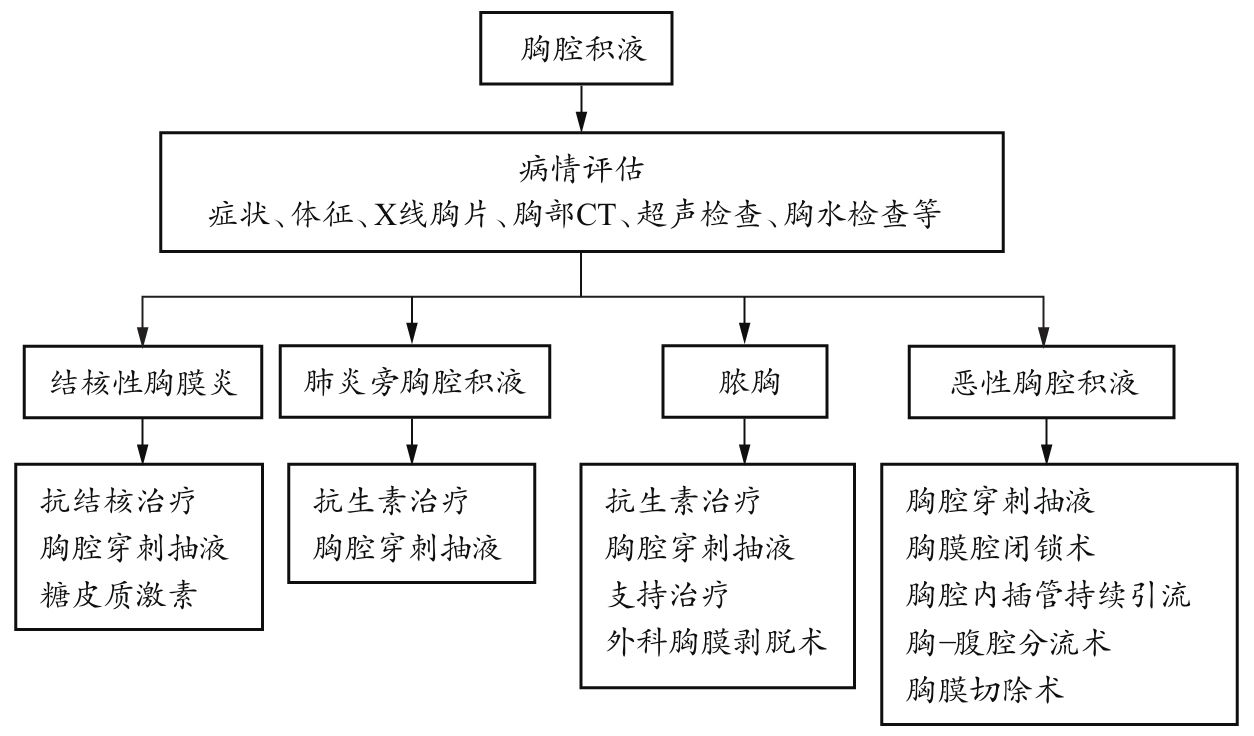
\includegraphics{./images/Image00037.jpg}
 \captionsetup{justification=centering}
 \caption{胸腔积液的治疗程序}
 \label{fig1-15-1}
  \end{figure} 

【治疗方案】

{(一)一般治疗}  包括休息、营养支持和对症治疗。

{(二)药物治疗}

1. 抗结核治疗 参见本章第十二节。

2.
糖皮质激素 用于结核性胸膜炎,但疗效不肯定。有全身毒性症状严重、大量胸水者,在抗结核药物治疗的同时,可尝试加用泼尼松30mg/d,分3次口服。待体温正常、全身毒性症状减轻、胸水量明显减少时,即应逐渐减量以至停用。停药速度不宜过快,否则易出现反跳现象,一般疗程4\textasciitilde{}6周。注意不良反应或结核播散,应慎重掌握适应证。

3.
抗生素治疗 肺炎旁胸腔积液的抗生素应用参见本章第九节。脓胸时抗菌药物要足量,体温恢复正常后再持续用药2周以上,防止脓胸复发,急性期联合抗厌氧菌的药物,全身及胸腔内给药。

{(三)胸腔穿刺引流治疗}
 由于结核性胸膜炎胸水蛋白含量高,容易引起胸膜粘连,原则上应尽快抽尽胸腔内积液或肋间插细管引流。可解除肺及心、血管受压,改善呼吸,使肺功能免受损伤。抽液后可减轻毒性症状,体温下降,有助于使被压迫的肺迅速复张。大量胸水者每周抽液2\textasciitilde{}3次,直至胸水完全消失。一般情况下,抽胸水后,没必要胸腔内注入抗结核药物,注入链激酶等可防止胸膜粘连。

肺炎旁胸腔积液,一般积液量少,经有效的抗生素治疗后可吸收。积液多者应胸腔穿刺抽液,胸水pH\textless{}7.2应肋间插管引流。

引流是脓胸最基本的治疗方法,反复抽脓或闭式引流。可用2\%碳酸氢钠或生理盐水反复冲洗胸腔,然后注入适量抗生素。少数脓胸可采用肋间插管闭式引流。对有支气管胸膜瘘者不宜冲洗胸腔,以免引起细菌播散。

恶性胸腔积液时,胸腔积液多为晚期恶性肿瘤常见并发症,其胸水生长迅速,常因大量积液的压迫引起严重呼吸困难,甚至导致死亡。常需反复胸腔穿刺抽液,但反复抽液可使蛋白丢失太多,效果不理想。此外,可胸腔内插管持续引流,目前多选用细管引流,具有创伤小、易固定、效果好、可随时胸腔内注入药物等优点。

{(四)其他治疗}

1. 慢性脓胸上述治疗效果不好的,可考虑外科胸膜剥脱术等治疗。

2.
恶性胸腔积液 ①注意原发病治疗。②可选择胸膜腔闭锁术,在抽吸胸水或胸腔插管引流后,胸腔内注入博来霉素、顺铂、丝裂霉素等抗肿瘤药物,或胸膜粘连剂,如滑石粉等,可减缓胸水的产生。也可胸腔内注入生物免疫调节剂,如短小棒状杆菌疫苗、白介素-2、干扰素、淋巴因子激活的杀伤细胞、肿瘤浸润性淋巴细胞等,可抑制恶性肿瘤细胞、增强淋巴细胞局部浸润及活性,并使胸膜粘连。③对插管引流后肺仍不复张者,可行胸腹腔分流术或胸膜切除术。

【疗效观察与随访】

1.
观察指标 观察治疗前后的呼吸困难、胸痛、咳嗽以及是否伴发热、消瘦、肝区疼痛等症状,观察胸膜摩擦感、胸膜摩擦音、触觉语颤、局部叩诊浊音,呼吸音等体征变化。

2.
疗效评估 一般原发疾病治愈,胸腔积液即可消失,如3个月未复发,即为痊愈。若为癌性胸腔积液早期术后可治愈,中晚期仅能缓解,甚至无效。

3. 随访 注意病情观察,确定原发病,避免并发症。

【治疗经验与解析】 胸腔穿刺引流治疗的并发症及处理要点:

(1)复张后肺水肿:胸腔穿刺引流治疗时,首次抽液不要超过700ml,以后每次抽液量不应超过1000ml,过快、过多抽液可使胸腔压力骤降,发生复张后肺水肿或循环衰竭。表现为剧咳、气促、咳大量泡沫状痰,双肺满布湿啰音,PaO{2}
下降,X线显示肺水肿征。应立即吸氧,酌情应用糖皮质激素及利尿剂,控制液体入量,严密监测病情与酸碱平衡,有时需气管插管机械通气。

(2)胸膜反应:若抽液时发生头晕、冷汗、心悸、面色苍白、脉细等表现应考虑胸膜反应,应立即停止抽液,使患者平卧,必要时皮下注射0.1\%肾上腺素0.5ml,密切观察病情,注意血压变化,防止休克。

(3)气胸:吸气时的胸腔内负压可能会导致气胸,注意一定要在患者处于呼气末时拔针。

\subsection{自发性气胸}

胸膜腔是不含气体的密闭的潜在性腔隙。当气体进入胸膜腔造成积气状态时,称为气胸(pneumothorax)。气胸可分成自发性气胸、创伤性气胸和人工气胸三类。气胸是常见的内科急症,男性多于女性,原发性气胸的发病率男性为18\textasciitilde{}28/10万人口,女性为1.2\textasciitilde{}6/10万人口。发生气胸后,胸膜腔内负压可变成正压,致使静脉回心血流受阻,产生程度不同的心、肺功能障碍。本节主要叙述自发性气胸。

【治疗程序】 图\ref{fig1-15-2}所示。

\begin{figure}[!htbp]
 \centering
 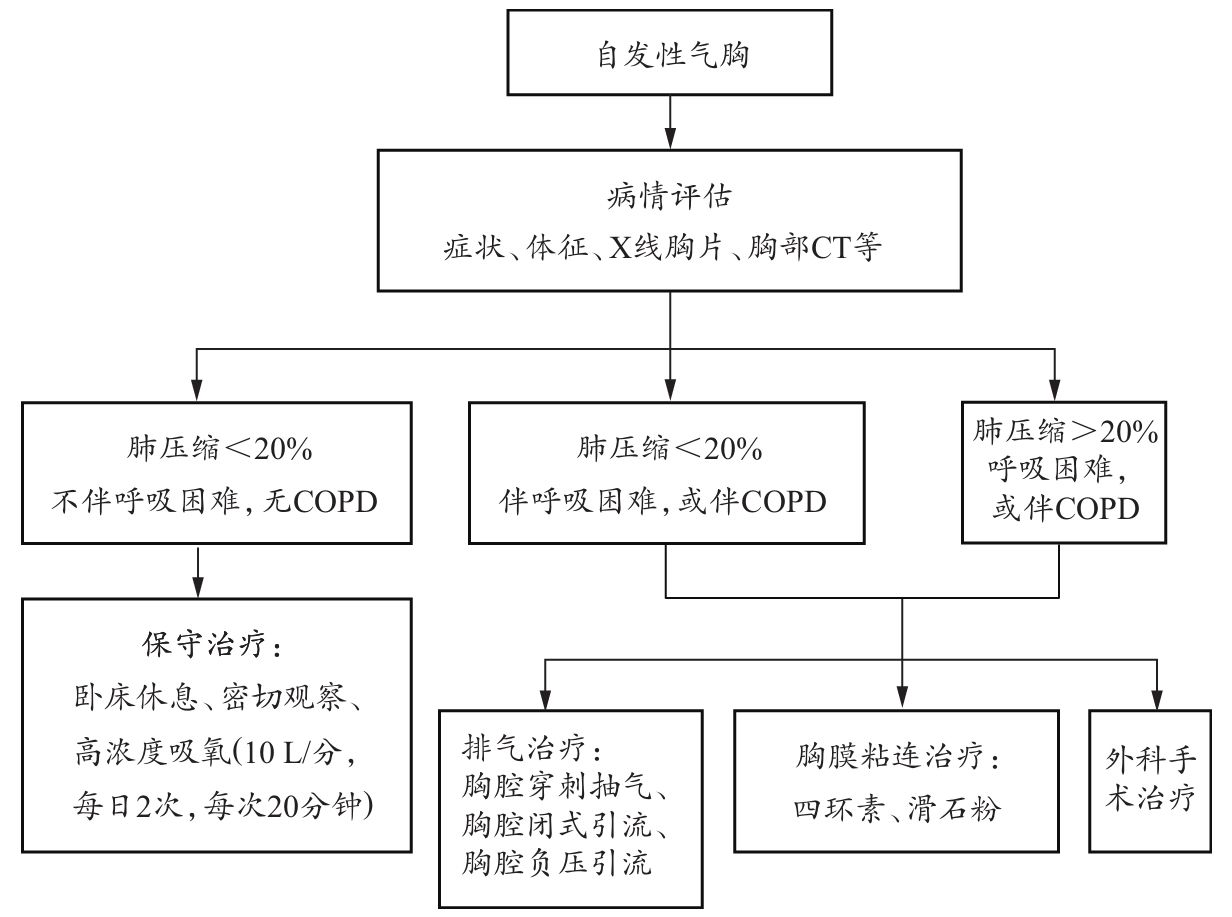
\includegraphics{./images/Image00038.jpg}
 \captionsetup{justification=centering}
 \caption{自发性气胸的治疗程序}
 \label{fig1-15-2}
  \end{figure} 

【治疗方案】

{(一)治疗原则}
 根据气胸的不同类型进行适当排气,以解除胸腔积气对呼吸、循环所造成的影响,使肺尽早复张,恢复功能,同时治疗原发病和并发症。

{(二)保守治疗}
 对于肺被压缩面积\textless{}20\%、单纯性、首次发生、无明显症状的闭合性气胸,可采用保守治疗。应严格卧床休息,酌情予镇静、镇痛等药物。高浓度吸氧可加快胸腔内气体的吸收,经鼻导管或面罩吸入10L/分的氧气,每日2次,每次20分钟,可达到比较满意的疗效。保守治疗需密切监测病情改变,尤其在气胸发生后24\textasciitilde{}48小时内。如患者年龄偏大,并有肺基础疾病如COPD,其胸膜破裂口愈合慢,呼吸困难等症状严重,即使气胸量较小,原则上不主张采取保守治疗。

此外,不可忽视肺基础疾病的治疗。如明确因肺结核并发气胸,应予抗结核药物;由肺部肿瘤所致气胸者,可先作胸腔闭式引流,待明确肿瘤的病理学类型及有无转移等情况后,再进一步作针对性治疗。COPD合并气胸者应注意积极控制肺部感染,解除气道痉挛等。

{(三)排气疗法}

1.
胸腔穿刺抽气 适用于肺被压缩面积\textgreater{}20\%,呼吸困难较轻,心肺功能尚好的闭合性气胸患者。肺压缩\textless{}20\%伴呼吸困难,或伴COPD者亦适用。抽气可加速肺复张,迅速缓解症状。通常选择患侧胸部锁骨中线第2肋间为穿刺点,局限性气胸则要选择相应的穿刺部位。皮肤消毒后用气胸针或细导管直接穿刺入胸腔,随后连接于50ml或100ml注射器或气胸机抽气并测压,直到患者呼吸困难缓解为止。一次抽气量不宜超过1000ml,每日或隔日抽气1次。张力性气胸病情危急,应迅速解除胸腔内正压以避免发生严重并发症,紧急时亦需立即胸腔穿刺排气,无其他抽气设备时,为了抢救患者生命,可用粗针头迅速刺入胸膜腔以达到暂时减压的目的。亦可用粗注射针头,在其尾部扎上橡皮指套,指套末端剪一小裂缝,插入胸腔做临时排气,高压气体从小裂缝排出,待胸腔内压减至负压时,套囊即行塌陷,小裂缝关闭,外界空气即不能进入胸膜腔。

2.
胸腔闭式引流 适用于不稳定型气胸,呼吸困难明显、肺压缩程度较重,交通性或张力性气胸,反复发生气胸的患者。无论其气胸容量多少,均应尽早行胸腔闭式引流。插管部位一般多取锁骨中线外侧第2肋间,或腋前线第4\textasciitilde{}5肋间,如为局限性气胸或需引流胸腔积液,则应根据X线胸片或在X线透视下选择适当部位进行插管排气引流。插管前,在选定部位先用气胸箱测压以了解气胸类型,然后在局麻下沿肋骨上缘平行作1.5\textasciitilde{}2cm皮肤切口,用套管针穿刺进入胸膜腔,拔去针芯,通过套管将灭菌胶管插入胸腔。亦可在切开皮肤后,经钝性分离肋间组织达胸膜,再穿破胸膜将导管直接送入胸膜腔。一般选用胸腔引流专用硅胶管,或外科胸腔引流管。16\textasciitilde{}22F导管适用于大多数患者,如有支气管胸膜瘘或机械通气的患者,应选择24\textasciitilde{}28F的大导管。导管固定后,另端可连接Heimhch单向活瓣,或置于水封瓶的水面下1\textasciitilde{}2cm,使胸膜腔内压力保持在1\textasciitilde{}2cmH{2}
O以下,插管成功则导管持续逸出气泡,呼吸困难迅速缓解,压缩的肺可在几小时至数天内复张。对肺压缩严重,时间较长的患者,插管后应夹住引流管分次引流,避免胸腔内压力骤降产生肺复张后肺水肿。如未见气泡逸出1\textasciitilde{}2日,患者气急症状消失,经透视或摄片见肺已全部复张时,可以拔除导管。有时虽未见气泡冒出水面,但患者症状缓解不明显,应考虑为导管不通畅,或部分滑出胸膜腔,需及时更换导管或作其他处理。

原发性自发性气胸经导管引流后,即可使肺完全复张;继发性者常因气胸分隔,单导管引流效果不佳,有时需在患侧胸腔插入多根导管。两侧同时发生气胸者,可在双侧胸腔作插管引流。若经水封瓶引流后未能使胸膜破口愈合,肺持久不能复张,可在引流管加用负压吸引装置。可用低负压可调节吸引机,如吸引机形成负压过大,可用调压瓶调节,一般负压为-10\textasciitilde{}-20cmH{2}
O,如果负压超过设置值,则空气由压力调节管进入调压瓶,因此胸腔所承受的吸引负压不会超过设置值,可避免过大的负压吸引对肺的损伤。

闭式负压吸引宜连续开动吸引机,如经12小时后肺仍未复张,应查找原因。如无气泡冒出,表示肺已复张,停止负压吸引,观察2\textasciitilde{}3日,经透视或胸片证实气胸未再复发后,即可拔除引流管,用凡士林纱布覆盖手术切口。

水封瓶应放在低于患者胸部的地方(如患者床下),以免瓶内的水反流进入胸腔。应用各式插管引流排气过程中,应注意严格消毒,防止发生感染。

{(四)胸膜粘连治疗}
 由于气胸复发率高,为了预防复发,可胸腔内注入硬化剂,产生无菌性胸膜炎症,使脏层和壁层胸膜粘连从而消灭胸膜腔间隙。主要适应于不宜手术或拒绝手术的下列患者:①持续性或复发性气胸;②双侧气胸;③合并肺大疱;④肺功能不全,不能耐受手术者。常用硬化剂有四环素、滑石粉、多西环素等,用生理盐水60\textasciitilde{}100ml稀释后经胸腔导管注入,夹管1\textasciitilde{}2小时后引流;或经胸腔镜直视下喷撒粉剂。胸腔注入硬化剂前,尽可能使肺完全复张。为避免药物引起的局部剧痛,先注入适量利多卡因,让患者转动体位,充分麻醉胸膜,15\textasciitilde{}20分钟后注入硬化剂。若一次无效,可重复注药。观察1\textasciitilde{}3日,经X线透视或摄片证实气胸已吸收,可拔除引流管。此法成功率高,主要不良反应为胸痛,发热,滑石粉可引起急性呼吸窘迫综合征,应用时应予注意。

{(五)手术治疗}
 经内科治疗无效的气胸可为手术的适应证,主要适应于长期气胸、血气胸、双侧气胸、复发性气胸、张力性气胸引流失败者、胸膜增厚致肺膨胀不全或影像学有多发性肺大疱者。手术治疗成功率高,复发率低。可行胸腔镜手术和开胸手术。

{(六)并发症及其处理}

1.
脓气胸 由金黄色葡萄球菌、肺炎克雷伯菌、铜绿假单胞菌、结核分枝杆菌以及多种厌氧菌引起的坏死性肺炎、肺脓肿以及干酪样肺炎可并发脓气胸,也可因胸穿或肋间插管引流所致。病情多危重,常有支气管胸膜瘘形成。脓液中可查到病原菌。除积极使用抗生素外,应插管引流,胸腔内生理盐水冲洗,必要时尚应根据具体情况考虑手术。

2.
血气胸 自发性气胸伴有胸膜腔内出血,常与胸膜粘连带内血管断裂有关,肺完全复张后,出血多能自行停止,若继续出血不止,除抽气排液及适当输血外,应考虑开胸结扎出血的血管。

3.
纵隔气肿与皮下气肿 由于肺泡破裂逸出的气体入肺间质,形成间质性肺气肿。肺间质内的气体沿血管鞘可进入纵隔,甚至进入胸部或腹部皮下组织,导致皮下气肿。张力性气胸抽气或闭式引流后,亦可沿针孔或切口出现胸壁皮下气肿,或全身皮下气肿及纵隔气肿。大多数患者并无症状,但颈部可因皮下积气而变粗。气体积聚在纵隔间隙可压迫纵隔大血管,出现干咳、呼吸困难、呕吐及胸骨后疼痛,并向双肩或双臂放射。疼痛常因呼吸运动及吞咽动作而加剧。患者发绀、颈静脉怒张、脉速、低血压、心浊音界缩小或消失、心音遥远、心尖部可听到清晰的与心跳同步的“卡嗒”声(Hamman征)。X线检查于纵隔旁或心缘旁(主要为左心缘)可见透明带。皮下气肿及纵隔气肿随胸腔内气体排出减压而自行吸收。吸入浓度较高的氧可增加纵隔内氧浓度,有利于气肿消散。若纵隔气肿张力过高影响呼吸及循环,可作胸骨上窝切开排气。

【疗效观察与随访】

1. 观察指标 常见症状与体征、胸部X线摄片变化及呼吸困难程度等。

2.
疗效评估 观察治疗前后症状体征变化,包括呼吸困难、胸痛、胸闷的程度,血流动力学变化,叩诊鼓音程度,呼吸音变化等。肺压缩\textless{}20\%患者保守治疗后,一般在7\textasciitilde{}14日自行吸收。

3.
随访 密切观察病情变化,缺氧征,注意胸片的及时复查,判断治疗效果。及时发现并积极处理并发症。

【治疗经验与解析】

1. 气胸的分类与治疗决策有关,不同类型气胸选择的治疗方法不同。

(1)根据病因分类:①自发性气胸:又可分成原发性和继发性,前者发生在无基础肺疾病的健康人,后者常发生在有基础肺疾病的患者,如慢性阻塞性肺疾病(COPD)、肺结核、肺囊性纤维化、支气管哮喘、间质性肺病、肺癌、尘肺、急性细菌性肺炎(金黄色葡萄球菌性肺炎)等。偶因胸膜上有异位子宫内膜,在经期可以破裂而发生气胸,称为月经性气胸。继发性自发性气胸在排气减压的同时,应积极治疗原发病;②创伤性气胸:系胸壁的直接或间接损伤脏层胸膜引起的气胸,如胸部锐器刺伤、枪弹的穿透伤或严重的挤压伤,以及医疗诊断和治疗操作过程中引起的气胸。常为血气胸;③人工气胸:系用人工方法将空气注入胸膜腔,以鉴别胸膜或肺内病变,或过去曾用于治疗肺结核等。实际上是创伤性气胸的一种特殊类型。

(2)按病程分类:①急性气胸:可采取保守治疗或胸腔抽气或引流治疗;②慢性气胸:保守治疗或胸腔抽气引流治疗往往效果不佳,可采用手术治疗;③复发性气胸:可采用胸膜粘连疗法,以防复发。

(3)按气胸合并积液的性质分类:①液(水)气胸:一般采用胸腔引流治疗;②血气胸:应胸腔引流,观察出血量,如内科治疗不能控制出血,应立即手术治疗;③脓气胸:必须进行胸腔引流或手术引流。

(4)按胸腔内压力类型分类:①闭合性(单纯性)气胸:应视肺压缩程度和基础肺功能情况,采取保守治疗、穿刺抽气或闭式引流术;②交通性(开放性)气胸:必须进行闭式引流;③张力性(高压性)气胸:一般先抽气降压,如无效则立即进行闭式引流术。

2.
继发性自发性气胸以COPD最常见,其次是肺结核。继发性自发性气胸时,由于基础肺功能较差,一般气急较明显,病情也较重,需高度重视,且抽气往往不能奏效,必须进行闭式引流术,疗程也比较长。气胸患者可伴有肿瘤、冠心病、高血压、糖尿病及营养不良等,在治疗时应进行相应的处理。合并冠心病者应保持有效的胸腔排气,应避免治疗诱发心绞痛的发生。合并糖尿病者容易发生肺、胸腔感染,在进行胸腔抽气或闭式引流术时必须严格无菌操作,适当使用抗生素控制感染。营养不良者发生气胸的创口较难愈合,在处理气胸的同时也要重视全身营养支持治疗。

3.
诱发气胸的因素较多,常见的原因如剧烈运动、咳嗽、提重物、举重、用力大便、屏气、打喷嚏、大笑、航空和潜水等。呼吸道感染也是常见诱发因素之一。因此,气胸患者应控制呼吸道感染,可适当使用镇咳药物,避免用力屏气动作,以避免发生或加重气胸。

4.
胸膜腔气体多少与治疗方法选择有关,肺压缩\textless{}20\%为少量气胸,20\%\textasciitilde{}40\%为中等量气胸,\textgreater{}40\%为大量气胸。少量气胸一般保守治疗,中等或大量气胸视病情,选择胸腔抽气或闭式引流术。

5.
患者的气急程度取决于发生气胸前基础肺病变及肺功能、气胸发生的速度、胸膜腔内积气量及压力,这是选择处理方法的重要依据。若气胸发生快、积气量大、基础肺功能差或张力性气胸,气急往往明显,应立即排气减压,缓解气急症状,必要时胸腔闭式引流。

6.
处理气胸应注意气胸引起的并发症以及治疗所引起的并发症,前者如纵隔气肿、张力性气胸引起血流动力学紊乱和呼吸循环障碍,双侧气胸引起通气和换气功能的严重障碍等。后者如气胸治疗可引起纵隔及皮下气肿、复张性肺水肿、脓气胸、血气胸、纵隔感染和胸腔感染等。治疗方案应针对各种并发症,如抗感染、抗休克、呼吸循环功能支持等。

\section{睡眠呼吸暂停综合征}

睡眠呼吸暂停综合征(sleep apnea
syndrome,SAS)是在睡眠时由多种病因引起反复发作的低通气或暂停,导致低氧、高碳酸血症和睡眠结构紊乱,导致白天嗜睡、心脑肺血管并发症乃至多脏器损害,是常见具有一定潜在危险的疾患,严重影响患者的生活质量和寿命。近年流行病学调查表明在国人中SAS的发病率约为4\%。SAS包括阻塞型睡眠呼吸暂停低通气综合征(obstructive
sleep apnea-hypopnea
syndrome,OSAHS)、中枢性睡眠呼吸暂停综合征(central sleep apnea
syndrome)、睡眠低通气综合征(sleep hypoventilation
syndrome)等。临床上以OSAHS最为常见,是多种全身疾患的独立危险因素。目前,由于对SAS的严重性、重要性和普遍性仍缺乏足够的认识,在临床诊疗中还常常不能做到早诊断、早治疗。

【治疗程序】 图\ref{fig1-16-1}\footnote{CPAP:持续气道正压通气;BiPAP:双水平气道正压通气;ASV:匹配伺服气道正压通气;UPPP:悬雍垂腭咽成形术}所示。

\begin{figure}[!htbp]
 \centering
 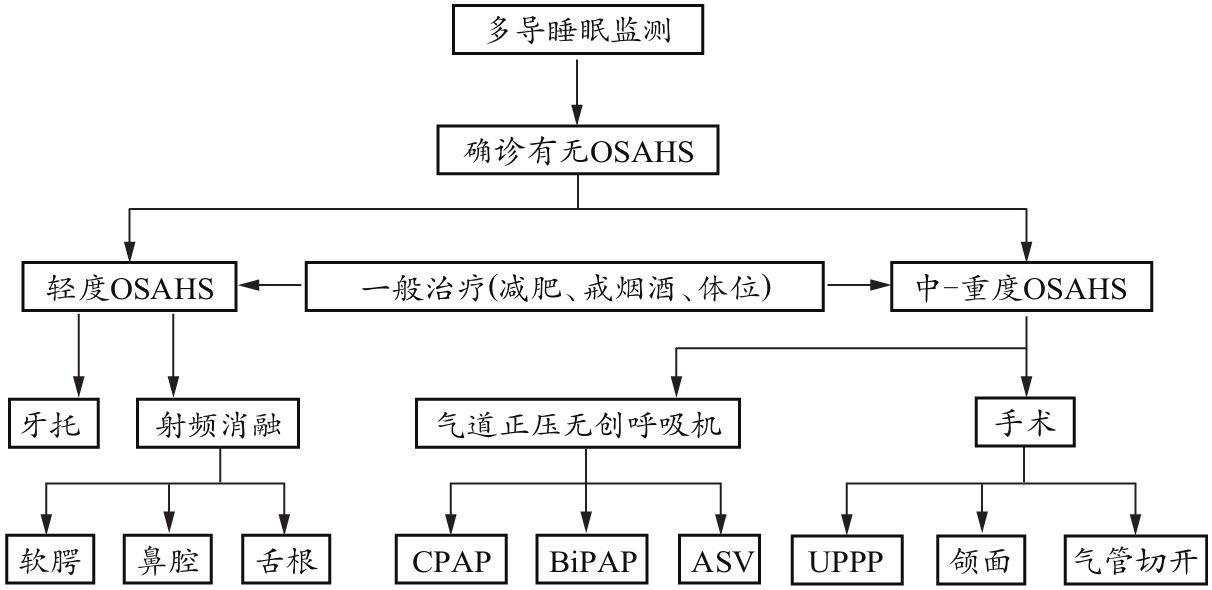
\includegraphics{./images/Image00039.jpg}
 \captionsetup{justification=centering}
 \caption{睡眠呼吸暂停综合征的治疗程序}
 \label{fig1-16-1}
  \end{figure} 

【治疗方案】

{(一)非手术疗法}

1.
减肥、调整睡姿、避免仰卧位、避免睡前饮酒和服用镇静剂 这些方法可以作为辅助治疗方法,有助于减轻症状,对于轻度睡眠呼吸暂停患者效果较好。

2. 气道内正压通气治疗 包括持续气道正压通气(continuous positive airway
pressure,CPAP)和双水平气道正压通气(bilevel positive airway
pressure,BiPAP),以经鼻CPAP(nCPAP)最为常用。如合并COPD即为重叠综合征,有条件者可用BiPAP。

(1)原理:提供一个生理性压力支撑上气道,以保证睡眠时上气道的开放。

(2)适应证:①OSAHS,特别是AHI在20次/小时以上者。②严重打鼾。③白天嗜睡而诊断不明者可进行试验性治疗。④OSAHS合并慢性阻塞性肺疾病(COPD)者,即“重叠综合征”。⑤OSAHS合并夜间哮喘。

(3)以下情况应慎用:①胸部X线或CT检查发现肺大疱。②气胸或纵隔气肿。③血压明显降低(血压低于90/60mmHg),或休克时。④急性心肌梗死患者血流动力学指标不稳定者。⑤脑脊液漏、颅脑外伤或颅内积气。⑥急性中耳炎、鼻炎、鼻窦炎感染未控制时。

(4)CPAP压力的调定:设定合适的CPAP压力水平是保证疗效的关键。理想的压力水平是指能够防止在各睡眠期及各种体位睡眠时出现的呼吸暂停所需的最低压力水平,同时这一压力值还能消除打鼾,并保持整夜睡眠中的血氧饱和度在正常水平(\textgreater{}90\%),并能为患者所接受。如用Auto
CPAP压力调定,选择90\%\textasciitilde{}95\%可信限的压力水平。①初始压力的设定:可以从较低的压力开始,如4\textasciitilde{}6cmH{2}
O,多数患者可以耐受。②CPAP压力的调定:临床观察。

3.
口腔矫正器或牙托 使下颌骨或舌体向前上方提起,从而增加咽部的横截面积,增加呼吸时的气流量。适用于轻度患者(AHI\textless{}15次/小时),特别是有下颌后缩者。对于不能耐受CPAP、不能手术或手术效果不佳者可以试用。禁忌证是患有颞颌关节炎或功能障碍。优点是无创伤、价格低,缺点是由于矫正器性能不同及患者的耐受情况不同,效果也不同。

4. 吸氧 吸氧可以改善低氧饱和度,但不能减少睡眠破坏和白天过度嗜睡。

5.
药物治疗 主要是通过改变睡眠结构和呼吸的神经控制功能,疗效尚不肯定,且有不同程度的不良反应。

(1)呼吸刺激剂:

乙酰唑胺:作为一种碳酸酐酶抑制剂,可诱导出代谢性酸中毒而刺激呼吸。该药治疗高原诱导的睡眠呼吸紊乱有效,也能改善陈施氏呼吸和其他类型的中枢性呼吸暂停。对阻塞性睡眠呼吸暂停患者的随机双盲研究提示乙酰唑胺可明显降低AHI,但监测最低血氧饱和度以及对≥4\%的氧减饱和度的次数提示患者的氧合状态并无变化,且从症状上看,这些患者并未感觉到睡眠质量和白日嗜睡有所改善。长期使用乙酰唑胺还存在耐受性差,且对OSAHS的疗效甚微。

甲羟孕酮(安宫黄体酮):作为一种呼吸刺激剂,已发现其能降低成年人的PaCO{2}
。绝经期前妇女由于体内雌激素的水平较高,OSAHS较为少见。因而认为雌激素对防止和减轻OSAHS可能具有保护性作用。曾有数个临床研究探讨了甲羟孕酮对OSAHS的效果,结果示疗效仍然甚微。

茶碱:是一种腺苷拮抗剂,具有刺激呼吸的作用。已有报道提示茶碱可减少中枢性呼吸暂停。由于氨茶碱的治疗窗窄,不良反应较明显,可使睡眠时间减少但并不能实质性地降低AHI,因此不被推荐为OSAHS的治疗药物。

总体看来,呼吸刺激剂虽然对减少中枢性呼吸暂停有效,但对缓解OSAHS无明显疗效。呼吸刺激剂可能增加对膈肌的呼吸驱动要强于对上气道扩张肌肉的驱动。由于在OSAHS患者中,对膈肌兴奋性的刺激实际上可能造成上气道管腔内负压更加明显,而诱发睡眠期上气道塌陷,从而抵消了其增加对上气道扩张肌的驱动而带来的有益处。

(2)促进Ⅲ/Ⅳ期睡眠或慢波睡眠的药物:OSAHS事件在慢波(Ⅲ/Ⅳ期)睡眠中较在浅NREM睡眠期或REM睡眠期中少见。因此又一类促进慢波睡眠的药物也被用于检验其对OSAHS的疗效。但迄今研究提示该类药对OSAHS并无总体的疗效,且因为有肌松作用不能推荐为OSAHS的临床用药。

(3)中枢神经系统刺激剂:莫达菲尼(Modafinil)是一种中枢神经系统的刺激剂,已发现该药能使OSAHS患者的白日嗜睡症状有所改善,但对OSAHS本身并无效果,因此不可能减少和防止OSAHS患者的心血管疾病发病率。

(4)5-羟色胺(5-HT)能制剂:5-HT药物,尤其是影响上气道运动神经元兴奋性的5-HT激动剂,在治疗OSAHS中是有效的。然而,5-HT对呼吸驱动的影响是复杂的,且已有资料显示5-HT拮抗剂的使用能增加舌下神经的兴奋性。5-HT拮抗增加呼吸驱动的调控可能在神经节,5-HT{2}
c或5-HT{3} 可能参与了此过程。有趣的是,5-HT{2} c兴奋剂和5-HT{3}
拮抗剂可减少正常大鼠的中枢性呼吸暂停。相反,5-HT{2}
c拮抗剂可导致英国喇叭犬发生阻塞性呼吸并可促进肥胖大鼠上气道发生塌陷。进一步研究需要确定5-HT的不同受体亚型在无论中枢还是外周呼吸调控中的作用,而且必须通过OSAHS的动物模型来阐明受体活动和功能的差异。

(5)药物治疗的发展方向:对OSAHS确实有效且安全的治疗药物仍期待被发掘。迄今对OSAHS的发病机制已有了较多的认识,但仍需要进一步阐明扩张上气道肌肉的兴奋性在清醒时增强而在睡眠时减弱的神经机制。其中首先应认识上气道运动神经元的状态依赖性神经化学调节机制,弄清有活性的5-HT受体亚型和其他神经化学介质。只有在进一步详细阐明了OSAHS的神经机制之后,才能明确OSAHS的药物治疗研究方向。对OSAHS进行成功的药物治疗还面临着巨大的挑战。

{(二)手术疗法}

1.
悬雍垂腭咽成形术(uvulopalatopharyngoplasty,UPPP) 手术切除悬雍垂、扁桃体和部分软腭,扩大口咽部气道。总有效率40\%(以AHI指数低于20为有效)。鼾声消失,但呼吸暂停仍存在。本手术有一定风险,另外2\%的患者术后吞咽及说话功能受到影响,50\%的患者术后需再行CPAP治疗。

2. 激光辅助悬雍垂软腭成形术(laser-assisted
uvulopalatoplasty,LAUP) 与传统的UPPP不同,LAUP仅切除部分腭垂和相应的软腭组织,可在门诊进行手术。

3.
气管切开术 治疗睡眠呼吸暂停的疗效确切,但对患者生理和心理的损害较大,仅适用于重度患者和经过其他治疗效果不佳者。气道造瘘:对于严重的OSAHS患者由于无法适应CPAP或BiPAP,或不适于行UPPP,或为防止UPPP手术及其他外科手术时发生意外可考虑进行气管造瘘。

4.
扁桃体切除术 儿童和青春期患者进行增殖腺与腭扁桃体切除有效,可改善患者的生长迟缓。成人仅行增殖腺和扁桃体切除无效,需与UPPP联用。

5. 颌面部手术 尚未普遍开展,其危险性和费用均较高,需随访。

6. 鼻部手术 可单独施行或与其他治疗方法联用,对鼻部阻塞患者有效。

7.
射频消融 为近年来开展的微创治疗,治疗部位可在鼻甲、软腭、舌根和扁桃腺,对轻度OSAHS有一定疗效,但长期疗效还有待观察。

8. 舌根部分切除术(舌根中线部分切除术) 对巨舌症患者有效。

【疗效观察与随访】

1.
观察指标 睡眠情况、自觉睡眠时呼吸暂停情况、CPAP压力测定胸部X线检查或CT检查及多导插记仪(PSG)监测等。

2. 治愈标准 症状、体征消失,PSG检查恢复正常,呼吸暂停指数\textless{}5。

3.
随访 对SAS的任何一种治疗方法,疗效评价和随访都是必需的。特别是不能省略和节约手术治疗后的PSG或初筛检查。随访应从治疗后的第1周开始,之后3个月、6个月和1年的定期随访应成为常规。随访主要内容包括:①有无坚持治疗及如何治疗?②还有无睡眠打鼾、憋气?必要时PSG复查;③SAS的症状如白日嗜睡有无及其程度(ESS评分法);④有无SAS的并发症如高血压、脑卒中、冠心病、糖尿病等及其程度。对CPAP使用患者定期随访是保证长期依从性的必要措施,观察发现随访组的依从性明显高于无随访组。研究表明,如果让1个SAS患者仅购买1台CPAP呼吸机而不予随诊指导,长期治疗的成功率较低,而随诊工作做得好,80\%的患者可得到有效的治疗。CPAP治疗随访过程中多不需要复查多导生理记录仪睡眠呼吸监测。对该类患者的随访,一方面有助于观察疗效和治疗反应,另一方面可以解决CPAP面罩、机械或使用问题。最初的CPAP建立以后,需有经过培训的健康治疗师对OSA患者进行1年1次的长期随访,以解决CPAP面罩、机械或使用问题。对于肥胖的SAS患者,有随访显示体重减低10\%往往可以使AHI降低近40\%\textasciitilde{}50\%。

【治疗经验与解析】 哪些OSAHS患者需要治疗?面对一个具体的患者如何恰当的确定治疗手段,目前为止还没有一个确切的回答和明确的标准。呼吸暂停低通气指数(AHI)是OSAHS诊断和分级的主要指标,而单纯的AHI并不能完全地反映病情的轻重,也不应该作为是否给予治疗和给予哪种治疗的唯一指标。应该说并非所有的OSAHS患者都需要治疗,治疗的人群应该和治疗目的相一致。为了划分病情的轻重在OSAHS诊断中确定了临床分级,分级的目的是评价病情和指导治疗,不同的分级程度应该有不同治疗措施。对于OSAHS严重程度的分级也经历了一个认识的过程,最初把AHI5\textasciitilde{}20定为轻度、AHI21\textasciitilde{}40为中度、AHI\textgreater{}40为重度。后来的调查发现,AHI高于15的患者已经出现心脑血管合并症,30以上的患者合并症的发生率和程度已经比较严重,因此把AHI为5\textasciitilde{}15定为轻度、AHI为16\textasciitilde{}30定为中度,将AHI\textgreater{}30确定为重度。一般来说,重度患者必须治疗,中度患者和日间有症状的轻度患者也需要治疗,近期的研究证实轻度患者治疗后同样收到良好效果。需要治疗的患者除了有明显的日间症状外,还倾向于包括那些易引发心脑血管疾病、影响生活质量和导致死亡率增加的人群。

美国睡眠学会的CPAP治疗适应证为:所有AHI大于15的患者,无论有无临床症状;AHI大于5有临床症状的患者,症状包括心脑血管疾病、日间嗜睡、失眠、性格和认知功能改变等。对CPAP和其他器械治疗依从性对保证治疗成功有重要作用。临床观察发现初用CPAP的不适感率高达80\%,因此提高治疗依从性对保证疗效至关重要。依从性主要决定于患者对CPAP治疗的意愿和疗效。噪音低、鼻罩柔软、密闭和湿化性能好、价格适宜等条件都会增加依从性。口腔矫治器的治疗同样有依从性问题。经验证明器械治疗的依从性有很强的可干预性,患者教育、CPAP首夜压力调定、充分解释和必要技术指导均有重要作用。在70\%的睡眠时间里,患者每夜使用CPAP少于4小时被定义为治疗失败。对这部分患者首先要询问和分析失败的原因,协助患者克服心理障碍和焦躁情绪、提高耐受性,尽可能地协助患者解除使用机器的不适感和CPAP引起的副作用。治疗失败后首先考虑的是不给予任何治疗患者危险性有多大,尤其是那些严重日间嗜睡和有严重多系统合并症伴日间低氧血症者。对仍不能接受CPAP治疗的轻、中度患者可以考虑口腔矫治器或颌面及咽部手术。

美国睡眠学会对各种治疗方法的疗效作了如下评价,气管插管和气管切开为100\%;持续气道正压通气(CPAP)为90\%;双水平正压通气(BiPAP)为95\%;扁桃体腭咽成形术(UPPP)为50\%\textasciitilde{}60\%;口腔矫治器为50\%\textasciitilde{}60\%;药物为20\%;氧疗为10\%;减肥为5\%。其中CPAP的疗效明显优于其他治疗,而且其判断有效的标准是AHI恢复正常范围、最低血氧饱和度\textgreater{}90\%,均优于其他治疗的有效标准。虽然气管插管和气管切开的疗效最佳,但是能接受和受益者甚少。

需要强调的是对重症OSAHS患者的UPPP手术尤其要慎重,必要时术前要做气管切开。应严格地按照手术的适应证确定治疗,应充分和客观地说明不同治疗方法的疗效和可能发生的合并症,尊重患者的选择和意愿,允许轻度患者有更多的选择。提倡手术与非手术科室和医生间的合作与协调,克服一味地强调某一种治疗而偏废其他治疗的倾向。由于多部位阻塞的高发生率和个体的差异应强调综合治疗的必要性,UPPP手术失败后的口腔矫治手术和多期的口和咽部手术的实施等。总之不应排斥任何安全和有助于提高疗效的措施。

多项实验显示了治疗SAS对心血管合并症有特异和无法取代的治疗作用。治疗可以预防和治疗患者合并的高血压、心力衰竭等心血管疾病已被大量的临床实验证实,而且治疗后全身和系统性炎症与氧化应激反应的减低是全身合并症好转和恢复的病理学基础。

\section{呼吸衰竭}

\subsection{急性肺损伤与急性呼吸窘迫综合征}

急性肺损伤(acute lung injury,ALI)和急性呼吸窘迫综合征(acute
respiratory distress
syndrome,ARDS)是在严重感染、休克、创伤及烧伤等疾病过程中,肺毛细血管内皮细胞和肺泡上皮细胞炎症性损伤造成弥漫性肺泡损伤,导致急性低氧性呼吸功能不全或衰竭。以肺容积减少、肺顺应性降低、严重的通气/血流比例失调为病理生理特征,临床上表现为进行性低氧血症和呼吸窘迫,肺部影像学上表现为非均一性的渗出性病变。ALI与ARDS是连续的病理生理过程。目前推荐的诊断标准包括:有ALI与ARDS的高危因素;急性发病、呼吸窘迫;X线胸片表现为双肺弥漫性渗出性改变;氧合指数(PaO{2}
/FiO{2}
)\textless{}300mmHg;肺动脉嵌顿压(PAWP)≤18mmHg,或无左心房高压的证据。达上述标准为ALI,而PaO{2}
/FiO{2} \textless{}200mmHg为ARDS。

【治疗程序】 图\ref{fig1-17-1}所示。

\begin{figure}[!htbp]
 \centering
 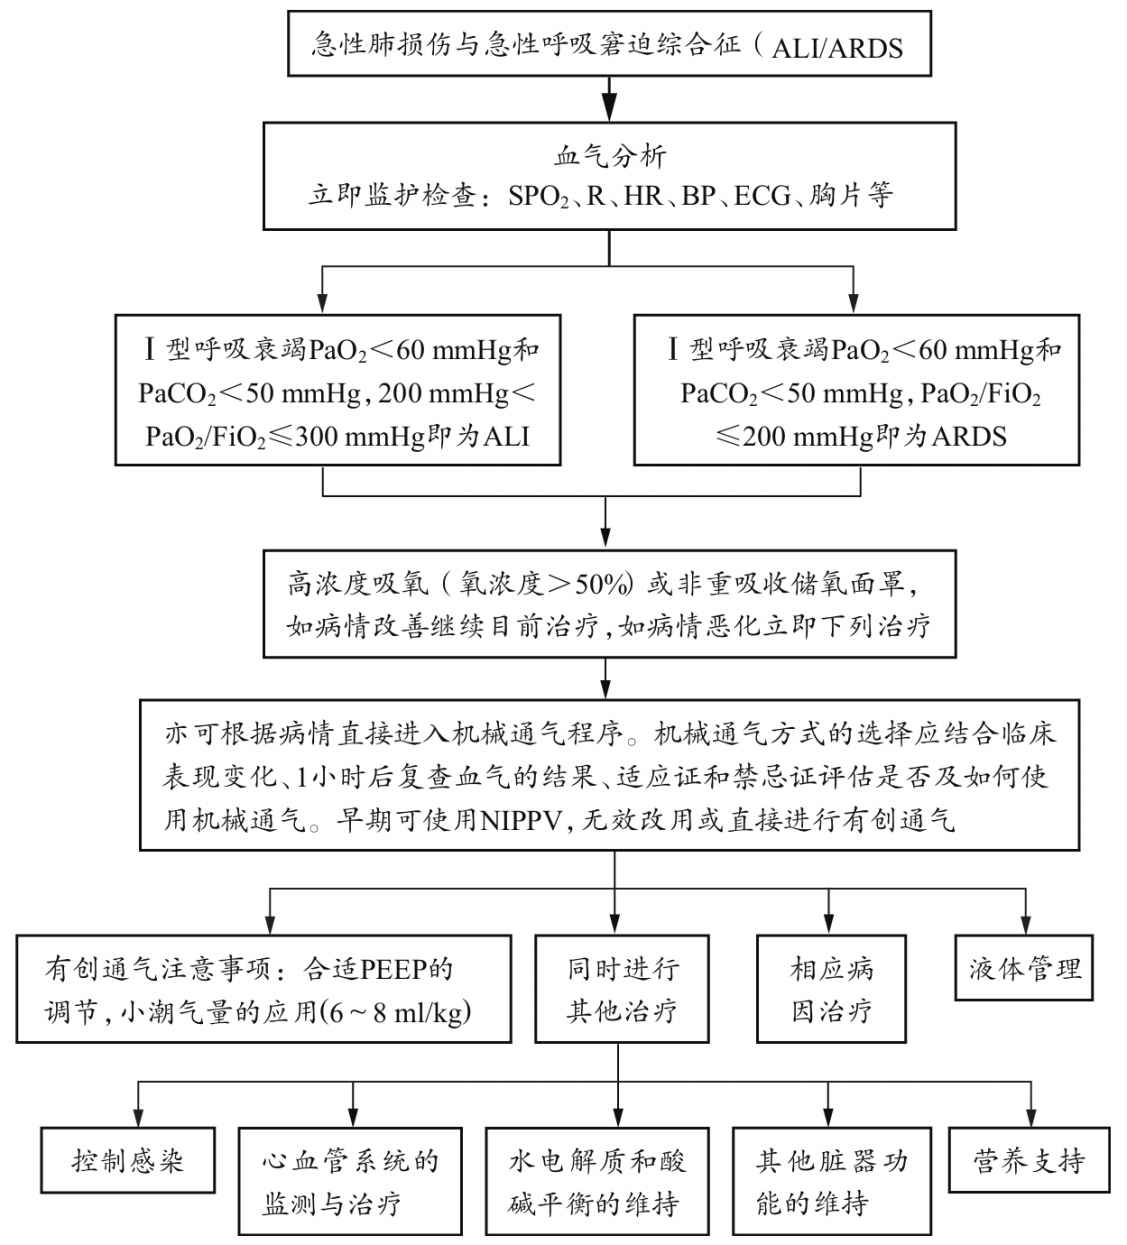
\includegraphics{./images/Image00040.jpg}
 \captionsetup{justification=centering}
 \caption{急性肺损伤和急性呼吸窘迫综合征的治疗程序}
 \label{fig1-17-1}
  \end{figure} 

【治疗方案】 ALI/ARDS是一种急性危重病,宜在严密监护下治疗。治疗的目标包括:改善肺氧合功能,纠正缺氧,生命支持,保护器官功能,防治并发症和基础病的治疗。

{(一)氧疗}
 纠正缺氧为刻不容缓的重要措施。一般需用高浓度给氧,才能使PaO{2}
\textgreater{}60mmHg或SaO{2}
\textgreater{}90\%。轻症者可用面罩给氧,但多数患者需用机械通气给氧。机械通气时给氧浓度恒定,且能与PEEP或CPAP同时应用。

{(二)机械通气}
 一旦诊断为ARDS,应尽早进行机械通气。早期轻症患者可试用无创性鼻(面)罩机械通气,但多数需要气管插管或切开作机械通气。

1.
现多应用肺保护性通气策略,要点包括:①应用合适的PEEP水平,避免呼气末肺泡及小气道闭陷。②用较低的潮气量(6ml/kg),限制吸气末气道峰压在35cmH{2}
O水平以下,平台压在25cmH{2} O水平以下。③允许PaCO{2} 高于正常水平。

2.
其他有可能改善肺氧合功能的通气模式还有:①双水平气道内正压。②反比通气。③俯卧位通气。④如仍不能维持必要的氧合,可使用体外膜氧合技术(ECMO)。

{(三)液体管理}
 保持循环系统较低的前负荷可减少肺水的含量,有报道可以缩短上机时间和降低死亡率。建议在早期可给予高渗晶体液,此后可给予胶体液,同时限制入量,辅以利尿剂,使出入量保持一定水平的负平衡,有条件可监测PAWP,在不影响心输出量和血压的情况下尽量降低PAWP。必要时可使用多巴胺和多巴酚丁胺等血管活性药物。

{(四)积极治疗基础疾病}

{(五)肺外脏器功能的支持和营养支持}
 近年来,呼吸支持技术的进步可使多数ARDS患者不再死于低氧血症,而主要死于MODS。ARDS可使肺外脏器功能受损,而肺外脏器功能受损又能反过来加重ARDS。因此,加强液体管理、尽早开始肠内营养、注意循环功能、肾功能和肝功能的支持对于防止MODS的发生有重要意义。

{(六)其他药物治疗}
 皮质激素在ARDS中应用争议较大,应根据病因及病情合理使用,在中晚期ARDS应用[1\textasciitilde{}2mg/(kg·d),维持2周,2周后逐渐减量]可能对防止肺纤维化有一定作用。对于脂肪栓综合征和肺孢子虫肺炎有预防或治疗作用。非皮质激素类抗炎症因子药物如乌斯他丁(每日60万\textasciitilde{}80万U)、血必净(每日100\textasciitilde{}200ml)等也可应用,但疗效不确切。

【疗效观察与随访】

1.
观察指标 常见症状与体征、呼吸状况、缺氧征、血气分析、血常规、血电解质、痰培养、X线胸片等。

2.
疗效评估 由于病因复杂,死亡率高达30\%\textasciitilde{}40\%,存活患者的生命质量仍可有一定损害。

3. 随访 密切观察病情变化,定期复查相关指标。恢复良好者,可随访5年。

【治疗经验与解析】

1.
ARDS患者应在监护病房中实行特别监护。动态监测呼吸、循环、水电解质、酸碱平衡及基础疾病,以便及时调整治疗方案。

2. 无创机械通气(NIPPV)

(1)NIPPV可以避免气管插管和气管切开引起的并发症,近年来得到了广泛的推广应用。迄今为止,尚无足够的资料显示NIPPV可以作为ALI/ARDS导致的急性低氧性呼吸衰竭的常规治疗方法。预计病情能够短期缓解的早期ALI/ARDS患者可考虑应用无创机械通气。应用NIPPV可使部分合并免疫抑制的ALI/ARDS患者避免有创机械通气,从而避免呼吸机相关肺炎(VAP)的发生,并可能改善预后。应用无创机械通气治疗ALI/ARDS应严密监测患者的生命体征及治疗反应。

(2)一般认为,ALI/ARDS患者在以下情况时不适宜应用NIPPV:①神志不清。②血流动力学不稳定。③气道分泌物明显增加而且气道自洁能力不足。④因脸部畸形、创伤或手术等不能佩戴鼻面罩。⑤上消化道出血、剧烈呕吐、肠梗阻和近期食管及上腹部手术。⑥危及生命的低氧血症。

(3)应用NIPPV治疗ALI/ARDS时应严密监测患者的生命体征及治疗反应。如NIPPV治疗1\textasciitilde{}2小时后,低氧血症和全身情况得到改善,可继续应用NIPPV。使用NIPPV过程中还需要密切监测患者腹部体征,防止压力过高导致腹胀;防止面罩过紧,而导致面部挤压伤;注意气道湿化,防止痰痂形成而阻塞气道。若低氧血症不能改善或全身情况恶化,提示NIPPV治疗失败,应及时改为有创通气。

3.
原发病是影响ARDS预后和转归的关键,及时去除或控制致病因素是ARDS治疗最关键的环节。主要包括充分引流感染灶、有效的清创和合理应用抗菌药物。腹腔、肺部感染的迁延,急性胰腺炎的发展等都使病因治疗相当困难。

4.
调控机体炎症反应 ARDS作为机体过度炎症反应的后果,SIRS是其根本原因,调控炎症反应不但是ARDS病因治疗的重要手段,而且也可能是控制ARDS、降低病死率的关键。

(1)糖皮质激素:是ARDS治疗中最富有争议的药物。目前不主张用大剂量激素,ARDS中晚期应用糖皮质激素[1\textasciitilde{}2mg/(kg·d),维持2周,2周后逐渐减量],有助于阻止肺纤维化的进展,可改善患者生存率;应用的同时必须监测患者病情,防止并发症或加重感染。

(2)重组人活化蛋白C(rhAPC或称Drotrecogin
alfa):具有抗血栓、抗炎和纤溶特性,已被试用于治疗严重感染。Ⅲ期临床试验证实,持续静脉注射rhAPC
24μg/(kg·h)×96小时,可以显著改善重度严重感染患者(APACHEⅡ\textgreater{}25)的预后。

5.
呼吸支持治疗可以纠正低氧血症,提高全身氧输送,防止组织缺氧,并尽早进行营养支持。早期积极的呼吸支持治疗,是纠正或改善顽固性低氧血症的关键手段,使患者不至死于早期严重的低氧血症,为治疗转机赢得时间。

6.
PEEP的选择要点 ARDS广泛肺泡塌陷不但可导致顽固的低氧血症,而且部分可复张的肺泡周期性塌陷开放而产生剪切力,会导致或加重呼吸机相关肺损伤。充分复张塌陷肺泡后应用适当水平PEEP防止呼气末肺泡塌陷,改善低氧血症,并避免剪切力,防治呼吸机相关肺损伤。因此,ARDS应采用能防止肺泡塌陷的最低PEEP。通过荟萃分析比较不同PEEP对ARDS患者生存率的影响,结果表明PEEP\textgreater{}12cmH{2}
O、尤其是\textgreater{}16cmH{2}
O时明显改善生存率。若有条件,应根据静态P-V曲线低位转折点压力+2cmH{2}
O来确定PEEP。除此之外,还有多种PEEP的选择方法,如氧合法、最大顺应性法、肺牵张指数法、氧输送法、CT法、依据静态压力-容积曲线吸气支低位拐点或呼气支拐点选择PEEP等方法。目前尚无足够证据支持何种方法选择最佳PEEP,在很大程度上依靠临床医生的经验。

7.
肺复张的要点 充分复张ARDS塌陷肺泡是纠正低氧血症和保证PEEP效应的重要手段。为限制气道平台压而被迫采取的小潮气量通气往往不利于ARDS塌陷肺泡的膨胀,而PEEP维持肺复张的效应依赖于吸气期肺泡的膨胀程度。目前临床常用的肺复张手法包括控制性肺膨胀、PEEP递增法及压力控制法(PCV法)。其中实施控制性肺膨胀采用恒压通气方式,推荐吸气压为30\textasciitilde{}45cmH{2}
O,持续时间30\textasciitilde{}40秒。

8.
自主呼吸要点 自主呼吸过程中膈肌主动收缩可增加ARDS患者肺重力依赖区的通气,改善通气血流比例失调,改善氧合。在循环功能稳定、人机协调性较好的情况下,ARDS患者机械通气时有必要保留自主呼吸。

9.
俯卧位通气要点 俯卧位通气通过降低胸腔内压力梯度、促进分泌物引流和促进肺内液体移动,明显改善氧合。应用高FiO{2}
或高气道平台压通气者,若体位改变无明显禁忌证,可采用俯卧位通气。患者在处于俯卧位状态下,必须经常检查气管插管的位置、中心静脉导管的位置、胸管的位置等,并且积极给予调整。对于合并有休克、室性或室上性心律失常等的血流动力学不稳定患者,存在颜面部创伤或未处理的不稳定性骨折的患者,为俯卧位通气的相对禁忌证。

10.
半卧位与VAP的预防 ARDS患者合并VAP往往使肺损伤进一步恶化,预防VAP具有重要的临床意义。机械通气患者平卧位易发生VAP。低于30°角的平卧位是院内获得性肺炎的独立危险因素。除非有脊髓损伤等体位改变的禁忌证,机械通气患者均应保持半卧位,预防VAP的发生。

11.
液体管理要点 液体管理是ARDS治疗的重要环节。在维持足够心排出量的前提下,通过利尿和适当限制输液量,保持较低前负荷,使PAWP不超过12mmHg是必要的。当然,应注意避免患者出现低血容量状态,导致心排出量降低和全身组织缺氧。一般主张在ARDS早期,肺毛细血管通透性明显增加的情况下,输注晶体液;当血清蛋白浓度降低时,可输注胶体液如血浆和羟甲淀粉(代血浆)制品,必要时应用白蛋白。

12.
呼吸机撤离与自主呼吸测试(SBT)要点 SBT的目的是评估患者是否可终止机械通气。进行SBT时应满足:①清醒。②血流动力学稳定(未使用升压药)。③无新的潜在严重病变。④需要低的通气条件及PEEP。⑤面罩或鼻导管吸氧可达到所需的PaO{2}
。如果SBT成功,则考虑拔管(见图\ref{fig1-17-2})。SBT可采用5cmH{2}
O的CPAP或T管进行,或低水平(依据气管插管的内径采用5\textasciitilde{}10cmH{2}
O)的PSV。

\begin{figure}[!htbp]
 \centering
 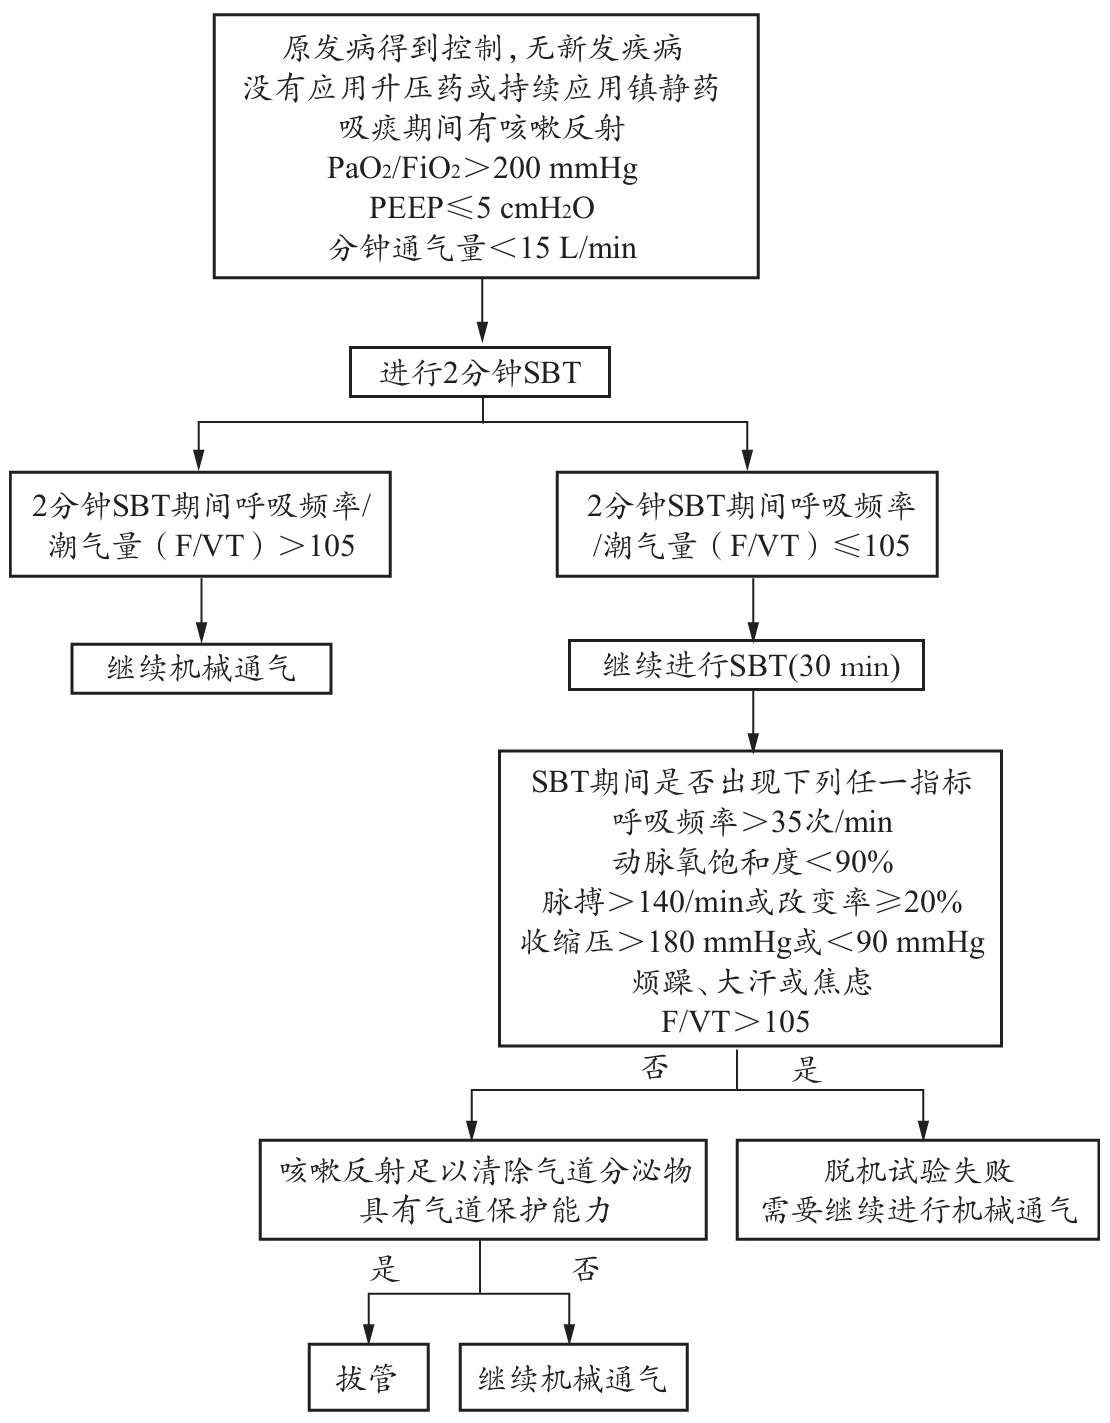
\includegraphics{./images/Image00041.jpg}
 \captionsetup{justification=centering}
 \caption{ARDS患者在脱机过程中SBT的实施程序}
 \label{fig1-17-2}
  \end{figure} 

13.
肺外器官功能支持是ARDS治疗不可忽视的重要环节。近年来,早期有力的呼吸支持使患者较少死于低氧血症,而主要死因是MODS。ARDS恶化可诱发或加重其他器官发生功能障碍、甚至衰竭,而肺外器官功能的衰竭反过来又可加重ARDS。加强肺外器官功能支持,防止MODS的发生和发展,可能是当前改善ARDS患者预后的重要手段。ARDS是MODS的一个重要组成部分,对ARDS的治疗是防治MODS的一部分。在进行ARDS呼吸功能支持和治疗的同时,不容忽视对循环功能、肾功能、肝功能等器官功能的监测和支持。

\subsection{慢性呼吸衰竭}

呼吸衰竭(respiratory
failure)是各种原因引起的肺通气和(或)换气功能严重障碍,最终导致动脉血氧分压(PaO{2}
)低于60mmHg,或伴有二氧化碳分压(PaCO{2}
)高于50mmHg,并排除心内解剖分流和原发于心排血量降低等因素,即为呼吸衰竭(简称呼衰)。按动脉血气分析分两种类型:①Ⅰ型:缺O{2}
而无CO{2} 潴留(PaO{2} \textless{}60mmHg,PaCO{2}
降低或正常)。②Ⅱ型:缺O{2} 伴CO{2} 潴留(PaO{2}
\textless{}60mmHg,PaCO{2}
\textgreater{}50mmHg)。慢性呼吸衰竭,是指一些慢性疾病,最常见的病因是慢性阻塞性肺疾病等,导致呼吸功能损害逐渐加重,经过较长时间才发展为呼衰。虽有缺O{2}
,或伴CO{2}
潴留,但通过机体代偿适应,生理功能障碍和代谢紊乱较轻。另一种临床较常见的情况是在慢性呼衰的基础上,因合并有呼吸系统感染或气道痉挛等情况,出现急性加重。在短时间内PaCO{2}
明显上升和PaO{2} 明显下降,称为慢性呼衰急性加重。

【治疗程序】 图\ref{fig1-17-3}所示。

\begin{figure}[!htbp]
 \centering
 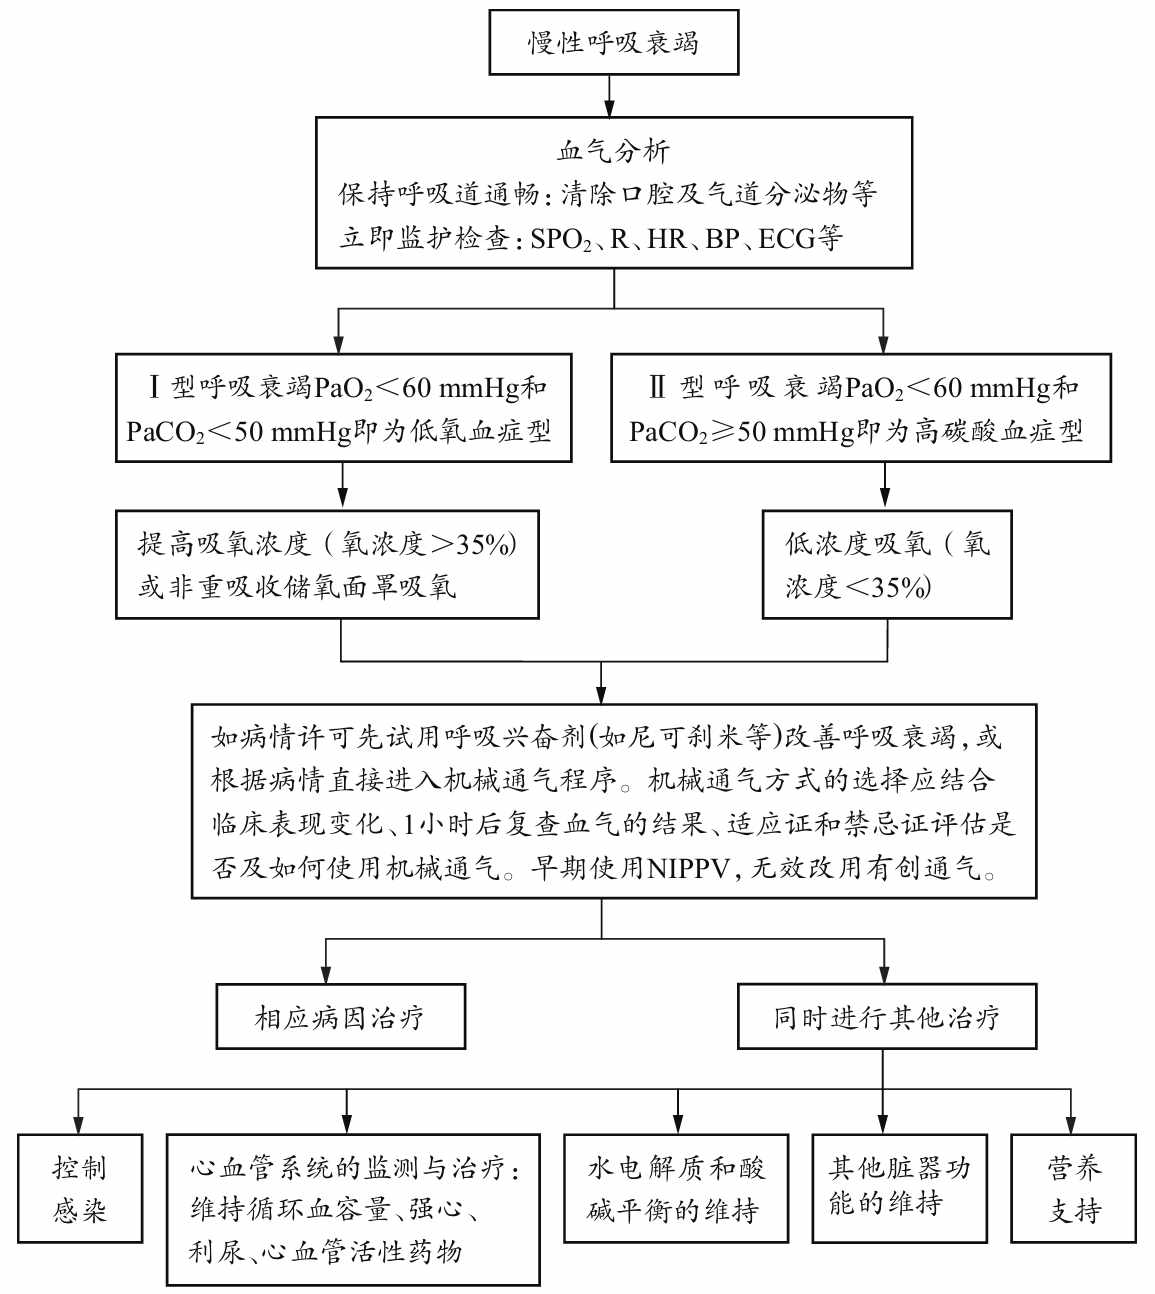
\includegraphics{./images/Image00042.jpg}
 \captionsetup{justification=centering}
 \caption{慢性呼吸衰竭的治疗程序}
 \label{fig1-17-3}
  \end{figure} 

【治疗方案】

{(一)呼衰处理的原则}
 是在保持呼吸道通畅条件下,改善通气和氧合功能,纠正缺O{2} 和CO{2}
潴留和代谢功能紊乱,防治多器官功能损害,从而为基础疾病和诱发因素的治疗争取时间和创造条件,但具体措施应结合患者的实际情况而定。

{(二)具体治疗措施}

1.
建立通畅的气道 包括清除口咽部及气道分泌物,盐酸氨溴索30\textasciitilde{}60mg静脉滴注每日3次促进排痰,氨茶碱每小时0.6\textasciitilde{}0.8mg/kg静脉滴注,可以维持有效血药浓度,从而扩张支气管,亦可用沙丁胺醇2ml、异丙托溴铵2ml、布地奈德2ml等单用或联用,每日2\textasciitilde{}3次射流雾化吸入舒张支气管。或用甲泼尼龙40\textasciitilde{}80mg静脉滴注每日1次舒张支气管等。病情危重者,可采用气管插管和气管切开建立人工气道。

2. 氧疗

(1)缺O{2} 不伴CO{2}
潴留的氧疗:应给予高浓度吸氧(\textgreater{}35\%),使PaO{2}
提高到60mmHg或SaO{2} 在90\%以上。

(2)缺O{2} 伴明显CO{2}
潴留的氧疗:氧疗原则应低浓度(\textless{}35\%)持续给氧。

3. 增加通气量、减少CO{2} 潴留

(1)合理使用呼吸兴奋剂,如尼可刹米(可拉明)每日1.875\textasciitilde{}3.75g静脉滴注等。

(2)机械通气对抢救呼衰患者常起关键作用:严重呼衰患者,如合并存在下列情况时,宜尽早建立人工气道,进行人工通气:①意识障碍,呼吸不规则。②气道分泌物多且有排痰障碍。③有较大的呕吐误吸的可能性,如球麻痹或腹胀呕吐者。④全身状态较差,疲乏明显者。⑤严重低氧血症或(和)CO{2}
潴留,达危及生命的程度(如PaO{2} ≤45mmHg,PacO{2}
≥70mmHg)。⑥合并多器官功能损害者。

人工气道的选择:最常用经口插管。近年采用面罩或鼻罩进行人工通气,在呼衰未发展到危重阶段尽早应用无创通气支持,有可能促进患者的康复,减少气管插管的需要。如用无创通气效果不佳者,再改用气管插管或切开。无创通气不宜用于昏迷、吞咽障碍、气道分泌物多,且伴清除障碍或伴多器官功能损害者。

4. 纠正酸碱平衡失调和电解质紊乱

(1)呼吸性酸中毒的治疗主要是改善肺泡通气量,一般不宜补碱。

(2)呼吸性酸中毒合并代谢性酸中毒治疗上应积极治疗代谢性酸中毒的病因,适量补碱,可用5\%碳酸氢钠50\textasciitilde{}100ml静脉滴注或缓慢静脉注射不宜急于将pH值调节至正常范围,否则有可能加重CO{2}
潴留。

(3)呼吸性酸中毒合并代谢性碱中毒治疗时应防止发生碱中毒的医源性因素和避免CO{2}
排出过快,并给予适量补氯和补钾,以缓解碱中毒。

5.抗感染治疗 呼吸道感染是呼衰最常见的诱因,根据经验性治疗及痰菌培养和药物敏感试验的结果,选择有效的药物控制呼吸道感染。

6.
合并症的防治 慢性肺源性心脏病、右心功能不全,急性加重时可能合并消化道出血、休克和多器官功能衰竭等,应积极防治。详见相关章节。

7.
营养支持 可用复方氨基酸250ml、中长链脂肪乳250ml、葡萄糖每日静脉滴注,同时可用肠内营养液:能全力、百普力、瑞能等每日1000\textasciitilde{}2000ml鼻饲,以保证每日有25\textasciitilde{}35kcal/kg的热量供应。

【疗效观察与随访】

1.
慢性呼吸衰竭治疗过程中要密切观察患者的生命体征、呼吸困难、氧合状态、血气分析的动态变化、神志状态等,根据病情变化及时调整治疗方案。

2.
AECOPD时慢性呼吸衰竭,如无禁忌证应首先使用无创机械通气,无创机械通气后均应测定血气分析,观察患者的生命体征、神志状态等及呼吸机通气参数:潮气量、压力、频率、吸气时间、漏气量等。有效者:临床上表现为气促改善、辅助呼吸肌肉动用减轻和反常呼吸消失、呼吸频率减慢、SaO{2}
增加,心率减慢等。如果没有上述临床改善,提示治疗效果差。通常建议治疗1\textasciitilde{}2小时后复查动脉血气。如果临床情况改善,PaCO{2}
下降\textgreater{}16\%,pH\textgreater{}7.30,PaO{2}
\textgreater{}40mmHg,提示初始治疗有效,建议继续无创通气治疗。否则应尽快调整治疗方案或改为插管人工通气,以免延误治疗的时机。对最终治疗成败的预测尚缺乏有效的指标。目前有限的资料显示,如果具有下列因素,提示无创通气的成功率低。这些因素包括:严重的呼吸衰竭、严重的肺炎、气道分泌物多、排痰能力差、患者不合作、严重酸血症(pH\textless{}7.20)、急性生理学慢性健康(APACHEⅡ)评分\textgreater{}15,治疗1\textasciitilde{}2小时后效果不明显等。

3.
无创机械通气应观察不良反应 呼吸困难加重、胃胀气、误吸、罩压迫、口咽干燥、鼻梁皮肤损伤、排痰障碍、不耐受/恐惧、睡眠性上气道阻塞等。并及时调整相应处理措施。

4.
关于无创机械通气疗程 有关每天治疗的时间和疗程,目前尚没有明确的标准。多数文献报道每次用3\textasciitilde{}6小时,每日1\textasciitilde{}3次。也有报道夜间睡眠时应用。急性呼吸衰竭治疗3\textasciitilde{}7日,慢性呼吸衰竭每天治疗\textgreater{}4小时,2个月后作疗效评价。如果有效者,可以长期应用。

5.
定期复查血常规、胸片、痰培养、血电解质酸碱状态、肝肾功能等,根据病情变化及时调整治疗方案。

6.
慢性呼吸衰竭往往是慢性疾病反复发展到终末状态的表现,由于慢性疾病不易控制导致慢性呼吸衰竭反复发生,预后往往较差。

【治疗经验与解析】

1.
恰当使用无创机械通气,由于无需气管插管或切开,能明显降低VAP的发生及呼吸机依赖。但应掌握好禁忌证。有绝对禁忌证的患者应该忌用NIPPV。然而,对于相对禁忌证,尚有待进一步探讨。在有比较好的监护条件和经验丰富的单位,在严密观察的前提下,可以作为探索性应用于有相对禁忌证的患者。

2.
无创机械通气参数的初始化和适应性调节要点:通气参数按照患者的具体情况来调节。为了提高舒适性和依从性,辅助通气的压力必须从较低的PSV压力水平或CPAP开始。通常吸气相压力从4\textasciitilde{}8cmH{2}
O、呼气相压力从2\textasciitilde{}3cmH{2}
O开始,经过5\textasciitilde{}20分钟逐渐增加到合适的治疗通气参数。如果一开始就用比较高的压力,患者会感觉不适而拒绝接受NIPPV;如果持续使用比较低的压力,则有可能达不到理想的辅助通气的效果,影响疗效。

3.
有创机械通气时通气量与频率的调节要点:建议采用f为15\textasciitilde{}25次/分钟,Vt为6\textasciitilde{}10ml/分钟,要求PaCO{2}
不高于60mmHg,pH大致正常即可。

4.
AECOPD由于呼气气流受限、呼气时间不足、呼吸机参数设置不当等原因产生PEEPi。PEEPi对患者存在不利影响:增加呼吸功、增加肺损伤的危险性、人机协调差、心功能不全、心律失常等。由于在COPD急性加重期,PEEPi的存在可产生上述不利影响,因此有效处理PEEPi具有重要意义。可通过以下措施来降低PEEPi:①降低患者的通气需要,如减轻患者的痛苦和紧张情绪、退热、减少糖类的摄入以降低CO{2}
的产生及应用镇静剂。②降低气道阻力:清除痰液保持呼吸道通畅;适当增加气管插管和呼吸管道的口径;扩张支气管,如应用β{2}
受体激动剂、茶碱、激素等药物。③改变呼吸机设置,如增加吸气流速、减少RR、降低VT及延长呼气时间等。

此外,PEEPe的应用可明显改善PEEPi对患者的不利影响,如减少呼吸功、改善人机协调性、改善肺泡通气及气体交换,但是如果PEEPe水平过高就会产生副作用,所以选择一个适宜水平的PEEPe以及根据病情调节PEEPe是一个重要问题。理想的PEEPe应是产生最好的生理效应、最小的副作用的最低水平的PEEPe,即“最佳PEEPe”。有三种常用的方法来设置PEEPe的大小:①根据所测PEEPi的大小加用PEEPe,PEEPe最大可加至所测PEEPi的75\%\textasciitilde{}85\%。②从低水平开始逐渐增加PEEPe的水平,同时监测吸气峰压和吸气平台压,以不引起吸气峰压和吸气平台压升高的最大PEEPe较为恰当。③也可从低水平逐渐加大PEEPe的水平,同时观察人机协调性,人机协调性最佳时的PEEPe水平比较合适。

5.
“有创”转换为“无创”的时机:重症COPD呼吸衰竭患者采用有创无创“序贯”MV的转换条件大体分为三类①以感染为主要诱发因素者,在肺部感染好转,呼吸肌疲劳恢复后,可提前拔管改用NIPPV。②以非感染因素为主要诱发因素者,可在诱因明确后尽早改用NIPPV。③因各种因素导致的一般情况较差或生命体征不稳定的患者,特别是长期气管插管的患者,则应在感染控制、一般情况明显好转的情况下,才能考虑改用NIPPV。当然,在前两种情况下应尽早实施,如有创MV后48\textasciitilde{}72小时。
